%********************************************%
%*       Generated from PreTeXt source      *%
%*       on 2026-07-16T19:36:21Z       *%
%*   A recent stable commit (2022-07-01):   *%
%* 6c761d3dba23af92cba35001c852aac04ae99a5f *%
%*                                          *%
%*         https://pretextbook.org          *%
%*                                          *%
%********************************************%
\documentclass[oneside,10pt,]{book}
%% Custom Preamble Entries, early (use latex.preamble.early)
%% Default LaTeX packages
%%   1.  always employed (or nearly so) for some purpose, or
%%   2.  a stylewriter may assume their presence
\usepackage{geometry}
%% Some aspects of the preamble are conditional,
%% the LaTeX engine is one such determinant
\usepackage{ifthen}
%% etoolbox has a variety of modern conveniences
\usepackage{etoolbox}
\usepackage{ifxetex,ifluatex}
%% Raster graphics inclusion
\usepackage{graphicx}
%% Color support, xcolor package
%% Always loaded, for: add/delete text, author tools
%% Here, since tcolorbox loads tikz, and tikz loads xcolor
\PassOptionsToPackage{dvipsnames,svgnames,table}{xcolor}
\usepackage{xcolor}
%% begin: defined colors, via xcolor package, for styling
%% end: defined colors, via xcolor package, for styling
%% Colored boxes, and much more, though mostly styling
%% skins library provides "enhanced" skin, employing tikzpicture
%% boxes may be configured as "breakable" or "unbreakable"
%% "raster" controls grids of boxes, aka side-by-side
\usepackage{tcolorbox}
\tcbuselibrary{skins}
\tcbuselibrary{breakable}
\tcbuselibrary{raster}
%% We load some "stock" tcolorbox styles that we use a lot
%% Placement here is provisional, there will be some color work also
%% First, black on white, no border, transparent, but no assumption about titles
\tcbset{ bwminimalstyle/.style={size=minimal, boxrule=-0.3pt, frame empty,
colback=white, colbacktitle=white, coltitle=black, opacityfill=0.0} }
%% Second, bold title, run-in to text/paragraph/heading
%% Space afterwards will be controlled by environment,
%% independent of constructions of the tcb title
%% Places \blocktitlefont onto many block titles
\tcbset{ runintitlestyle/.style={fonttitle=\blocktitlefont\upshape\bfseries, attach title to upper} }
%% Spacing prior to each exercise, anywhere
\tcbset{ exercisespacingstyle/.style={before skip={1.5ex plus 0.5ex}} }
%% Spacing prior to each block
\tcbset{ blockspacingstyle/.style={before skip={2.0ex plus 0.5ex}} }
%% xparse allows the construction of more robust commands,
%% this is a necessity for isolating styling and behavior
%% The tcolorbox library of the same name loads the base library
\tcbuselibrary{xparse}
%% The tcolorbox library loads TikZ, its calc package is generally useful,
%% and is necessary for some smaller documents that use partial tcolor boxes
%% See:  https://github.com/PreTeXtBook/pretext/issues/1624
\usetikzlibrary{calc}
%% We use some more exotic tcolorbox keys to restore indentation to parboxes
\tcbuselibrary{hooks}
%% Save default paragraph indentation and parskip for use later, when adjusting parboxes
\newlength{\normalparindent}
\newlength{\normalparskip}
\AtBeginDocument{\setlength{\normalparindent}{\parindent}}
\AtBeginDocument{\setlength{\normalparskip}{\parskip}}
\newcommand{\setparstyle}{\setlength{\parindent}{\normalparindent}\setlength{\parskip}{\normalparskip}}%% Hyperref should be here, but likes to be loaded late
%%
%% Inline math delimiters, \(, \), need to be robust
%% 2016-01-31:  latexrelease.sty  supersedes  fixltx2e.sty
%% If  latexrelease.sty  exists, bugfix is in kernel
%% If not, bugfix is in  fixltx2e.sty
%% See:  https://tug.org/TUGboat/tb36-3/tb114ltnews22.pdf
%% and read "Fewer fragile commands" in distribution's  latexchanges.pdf
\IfFileExists{latexrelease.sty}{}{\usepackage{fixltx2e}}
%% shorter subnumbers in some side-by-side require manipulations
\usepackage{xstring}
%% Text height identically 9 inches, text width varies on point size
%% See Bringhurst 2.1.1 on measure for recommendations
%% 75 characters per line (count spaces, punctuation) is target
%% which is the upper limit of Bringhurst's recommendations
\geometry{letterpaper,total={340pt,9.0in}}
%% Custom Page Layout Adjustments (use publisher page-geometry entry)
%% This LaTeX file may be compiled with pdflatex, xelatex, or lualatex executables
%% LuaTeX is not explicitly supported, but we do accept additions from knowledgeable users
%% The conditional below provides  pdflatex  specific configuration last
%% begin: engine-specific capabilities
\ifthenelse{\boolean{xetex} \or \boolean{luatex}}{%
%% begin: xelatex and lualatex-specific default configuration
\ifxetex\usepackage{xltxtra}\fi
%% realscripts is the only part of xltxtra relevant to lualatex 
\ifluatex\usepackage{realscripts}\fi
%% end:   xelatex and lualatex-specific default configuration
}{
%% begin: pdflatex-specific default configuration
%% We assume a PreTeXt XML source file may have Unicode characters
%% and so we ask LaTeX to parse a UTF-8 encoded file
%% This may work well for accented characters in Western language,
%% but not with Greek, Asian languages, etc.
%% When this is not good enough, switch to the  xelatex  engine
%% where Unicode is better supported (encouraged, even)
\usepackage[utf8]{inputenc}
%% end: pdflatex-specific default configuration
}
%% end:   engine-specific capabilities
%%
%% Fonts.  Conditional on LaTex engine employed.
%% Default Text Font: The Latin Modern fonts are
%% "enhanced versions of the [original TeX] Computer Modern fonts."
%% We use them as the default text font for PreTeXt output.
%% Default Monospace font: Inconsolata (aka zi4)
%% Sponsored by TUG: http://levien.com/type/myfonts/inconsolata.html
%% Loaded for documents with intentional objects requiring monospace
%% See package documentation for excellent instructions
%% fontspec will work universally if we use filename to locate OTF files
%% Loads the "upquote" package as needed, so we don't have to
%% Upright quotes might come from the  textcomp  package, which we also use
%% We employ the shapely \ell to match Google Font version
%% pdflatex: "varl" package option produces shapely \ell
%% pdflatex: "var0" package option produces plain zero (not used)
%% pdflatex: "varqu" package option produces best upright quotes
%% xelatex,lualatex: add OTF StylisticSet 1 for shapely \ell
%% xelatex,lualatex: add OTF StylisticSet 2 for plain zero (not used)
%% xelatex,lualatex: add OTF StylisticSet 3 for upright quotes
%%
%% Automatic Font Control
%% Portions of a document, are, or may, be affected by defined commands
%% These are perhaps more flexible when using  xelatex  rather than  pdflatex
%% The following definitions are meant to be re-defined in a style, using \renewcommand
%% They are scoped when employed (in a TeX group), and so should not be defined with an argument
\newcommand{\divisionfont}{\relax}
\newcommand{\blocktitlefont}{\relax}
\newcommand{\contentsfont}{\relax}
\newcommand{\pagefont}{\relax}
\newcommand{\tabularfont}{\relax}
\newcommand{\xreffont}{\relax}
\newcommand{\titlepagefont}{\relax}
%%
\ifthenelse{\boolean{xetex} \or \boolean{luatex}}{%
%% begin: font setup and configuration for use with xelatex
%% Generally, xelatex is necessary for non-Western fonts
%% fontspec package provides extensive control of system fonts,
%% meaning *.otf (OpenType), and apparently *.ttf (TrueType)
%% that live *outside* your TeX/MF tree, and are controlled by your *system*
%% (it is possible that a TeX distribution will place fonts in a system location)
%%
%% The fontspec package is the best vehicle for using different fonts in  xelatex
%% So we load it always, no matter what a publisher or style might want
%%
\usepackage{fontspec}
%%
%% begin: xelatex main font ("font-xelatex-main" template)
%% Latin Modern Roman is the default font for xelatex and so is loaded with a TU encoding
%% *in the format* so we can't touch it, only perhaps adjust it later
%% in one of two ways (then known by NFSS names such as "lmr")
%% (1) via NFSS with font family names such as "lmr" and "lmss"
%% (2) via fontspec with commands like \setmainfont{Latin Modern Roman}
%% The latter requires the font to be known at the system-level by its font name,
%% but will give access to OTF font features through optional arguments
%% https://tex.stackexchange.com/questions/470008/
%% where-and-how-does-fontspec-sty-specify-the-default-font-latin-modern-roman
%% http://tex.stackexchange.com/questions/115321
%% /how-to-optimize-latin-modern-font-with-xelatex
%%
%% end:   xelatex main font ("font-xelatex-main" template)
%% begin: xelatex math font ("font-xelatex-math" template)
%% end:   xelatex math font ("font-xelatex-math" template)
%% begin: xelatex mono font ("font-xelatex-mono" template)
%% (conditional on non-trivial uses being present in source)
\IfFontExistsTF{Inconsolatazi4-Regular.otf}{}{\GenericError{}{The font "Inconsolatazi4-Regular.otf" requested by PreTeXt output processed by the  xelatex  executable is not available.  Either a file cannot be located in default locations via a filename, or a font is not known by its name as part of your system.}{Consult the PreTeXt Guide for help with LaTeX fonts, or perhaps try using  pdflatex  as a test.}{}}
\IfFontExistsTF{Inconsolatazi4-Bold.otf}{}{\GenericError{}{The font "Inconsolatazi4-Bold.otf" requested by PreTeXt output processed by the  xelatex  executable is not available.  Either a file cannot be located in default locations via a filename, or a font is not known by its name as part of your system.}{Consult the PreTeXt Guide for help with LaTeX fonts, or perhaps try using  pdflatex  as a test.}{}}
\usepackage{zi4}
\setmonofont[BoldFont=Inconsolatazi4-Bold.otf,StylisticSet={1,3}]{Inconsolatazi4-Regular.otf}
%% end:   xelatex mono font ("font-xelatex-mono" template)
%% begin: xelatex font adjustments ("font-xelatex-style" template)
%% end:   xelatex font adjustments ("font-xelatex-style" template)
%%
%% Extensive support for other languages
\usepackage{polyglossia}
%% Set main/default language based on pretext/@xml:lang value
%% document language code is "en-US", US English
%% usmax variant has extra hypenation
\setmainlanguage[variant=usmax]{english}
%% Enable secondary languages based on discovery of @xml:lang values
%% Enable fonts/scripts based on discovery of @xml:lang values
%% Western languages should be ably covered by Latin Modern Roman
%% end:   font setup and configuration for use with xelatex
}{%
%% begin: font setup and configuration for use with pdflatex
%% begin: pdflatex main font ("font-pdflatex-main" template)
\usepackage{lmodern}
\usepackage[T1]{fontenc}
%% end:   pdflatex main font ("font-pdflatex-main" template)
%% begin: pdflatex mono font ("font-pdflatex-mono" template)
%% (conditional on non-trivial uses being present in source)
\usepackage[varqu,varl]{inconsolata}
%% end:   pdflatex mono font ("font-pdflatex-mono" template)
%% begin: pdflatex font adjustments ("font-pdflatex-style" template)
%% end:   pdflatex font adjustments ("font-pdflatex-style" template)
%% end:   font setup and configuration for use with pdflatex
}
%% Micromanage spacing, etc.  The named "microtype-options"
%% template may be employed to fine-tune package behavior
\usepackage{microtype}
%% Symbols, align environment, commutative diagrams, bracket-matrix
\usepackage{amsmath}
\usepackage{amscd}
\usepackage{amssymb}
%% allow page breaks within display mathematics anywhere
%% level 4 is maximally permissive
%% this is exactly the opposite of AMSmath package philosophy
%% there are per-display, and per-equation options to control this
%% split, aligned, gathered, and alignedat are not affected
\allowdisplaybreaks[4]
%% allow more columns to a matrix
%% can make this even bigger by overriding with  latex.preamble.late  processing option
\setcounter{MaxMatrixCols}{30}
%%
%% Symbols for use in text mode (i.e. not in math mode)
\usepackage{pifont}
%% Solid geometric shapes to mark ends of environments
\newcommand{\ptxsquare}{\ding{110}}
\newcommand{\ptxtriangle}{\ding{115}}
\newcommand{\ptxdiamond}{\ding{117}}
%% Markers for unordered list items
\newcommand{\ptxlistdisc}{\raisebox{0.3ex}{\textbullet}}
\newcommand{\ptxlistcircle}{\raisebox{0.3ex}{\textopenbullet}}
\newcommand{\ptxlistsquare}{\raisebox{0.4ex}{\scalebox{0.5}{\ding{110}}}}
%%
%% Division Titles, and Page Headers/Footers
%% titlesec package, loading "titleps" package cooperatively
%% See code comments about the necessity and purpose of "explicit" option.
%% The "newparttoc" option causes a consistent entry for parts in the ToC 
%% file, but it is only effective if there is a \titleformat for \part.
%% "pagestyles" loads the  titleps  package cooperatively.
\usepackage[explicit, newparttoc, pagestyles]{titlesec}
%% The companion titletoc package for the ToC.
\usepackage{titletoc}
%% Fixes a bug with transition from chapters to appendices in a "book"
%% See generating XSL code for more details about necessity
\newtitlemark{\chaptertitlename}
%% begin: customizations of page styles via the modal "titleps-style" template
%% Designed to use commands from the LaTeX "titleps" package
%% Plain pages should have the same font for page numbers
\renewpagestyle{plain}{%
\setfoot{}{\pagefont\thepage}{}%
}%
%% Single pages as in default LaTeX
\renewpagestyle{headings}{%
\sethead{\pagefont\slshape\MakeUppercase{\ifthechapter{\chaptertitlename\space\thechapter.\space}{}\chaptertitle}}{}{\pagefont\thepage}%
}%
\pagestyle{headings}
%% end: customizations of page styles via the modal "titleps-style" template
%%
%% Create globally-available macros to be provided for style writers
%% These are redefined for each occurence of each division
\newcommand{\divisionnameptx}{\relax}%
\newcommand{\titleptx}{\relax}%
\newcommand{\subtitleptx}{\relax}%
\newcommand{\shortitleptx}{\relax}%
\newcommand{\authorsptx}{\relax}%
\newcommand{\epigraphptx}{\relax}%
%% Create environments for possible occurences of each division
%% Environment for a PTX "chapter" at the level of a LaTeX "chapter"
\NewDocumentEnvironment{chapterptx}{mmmmmmm}
{%
\renewcommand{\divisionnameptx}{#1}%
\renewcommand{\titleptx}{#2}%
\renewcommand{\subtitleptx}{#3}%
\renewcommand{\shortitleptx}{#4}%
\renewcommand{\authorsptx}{#5}%
\renewcommand{\epigraphptx}{#6}%
\chapter[{#4}]{#2}%
\label{#7}%
}{}%
%% Environment for a PTX "section" at the level of a LaTeX "section"
\NewDocumentEnvironment{sectionptx}{mmmmmmm}
{%
\renewcommand{\divisionnameptx}{#1}%
\renewcommand{\titleptx}{#2}%
\renewcommand{\subtitleptx}{#3}%
\renewcommand{\shortitleptx}{#4}%
\renewcommand{\authorsptx}{#5}%
\renewcommand{\epigraphptx}{#6}%
\section[{#4}]{#2}%
\label{#7}%
}{}%
%% Environment for a PTX "exercises" at the level of a LaTeX "subsection"
\NewDocumentEnvironment{exercises-subsection}{mmmmmmm}
{%
\renewcommand{\divisionnameptx}{#1}%
\renewcommand{\titleptx}{#2}%
\renewcommand{\subtitleptx}{#3}%
\renewcommand{\shortitleptx}{#4}%
\renewcommand{\authorsptx}{#5}%
\renewcommand{\epigraphptx}{#6}%
\subsection[{#4}]{#2}%
\label{#7}%
}{}%
%% Environment for a PTX "exercises" at the level of a LaTeX "subsection"
\NewDocumentEnvironment{exercises-subsection-numberless}{mmmmmmm}
{%
\renewcommand{\divisionnameptx}{#1}%
\renewcommand{\titleptx}{#2}%
\renewcommand{\subtitleptx}{#3}%
\renewcommand{\shortitleptx}{#4}%
\renewcommand{\authorsptx}{#5}%
\renewcommand{\epigraphptx}{#6}%
\subsection*{#2}%
\addcontentsline{toc}{subsection}{#4}
\label{#7}%
}{}%
%% Environment for a PTX "subsection" at the level of a LaTeX "subsection"
\NewDocumentEnvironment{subsectionptx}{mmmmmmm}
{%
\renewcommand{\divisionnameptx}{#1}%
\renewcommand{\titleptx}{#2}%
\renewcommand{\subtitleptx}{#3}%
\renewcommand{\shortitleptx}{#4}%
\renewcommand{\authorsptx}{#5}%
\renewcommand{\epigraphptx}{#6}%
\subsection[{#4}]{#2}%
\label{#7}%
}{}%
%% Environment for a PTX "worksheet" at the level of a LaTeX "section"
\NewDocumentEnvironment{worksheet-section}{mmmmmmm}
{%
\renewcommand{\divisionnameptx}{#1}%
\renewcommand{\titleptx}{#2}%
\renewcommand{\subtitleptx}{#3}%
\renewcommand{\shortitleptx}{#4}%
\renewcommand{\authorsptx}{#5}%
\renewcommand{\epigraphptx}{#6}%
\section[{#4}]{#2}%
\label{#7}%
}{}%
%% Environment for a PTX "worksheet" at the level of a LaTeX "section"
\NewDocumentEnvironment{worksheet-section-numberless}{mmmmmmm}
{%
\renewcommand{\divisionnameptx}{#1}%
\renewcommand{\titleptx}{#2}%
\renewcommand{\subtitleptx}{#3}%
\renewcommand{\shortitleptx}{#4}%
\renewcommand{\authorsptx}{#5}%
\renewcommand{\epigraphptx}{#6}%
\section*{#2}%
\addcontentsline{toc}{section}{#4}
\label{#7}%
}{}%
%%
%% Styles for six traditional LaTeX divisions
\titleformat{\part}[display]
{\divisionfont\Huge\bfseries\centering}{\divisionnameptx\space\thepart}{30pt}{\Huge#1}
[{\Large\centering\authorsptx}]
\titleformat{\chapter}[display]
{\divisionfont\huge\bfseries}{\divisionnameptx\space\thechapter}{20pt}{\Huge#1}
[{\Large\authorsptx}]
\titleformat{name=\chapter,numberless}[display]
{\divisionfont\huge\bfseries}{}{0pt}{#1}
[{\Large\authorsptx}]
\titlespacing*{\chapter}{0pt}{50pt}{40pt}
\titleformat{\section}[hang]
{\divisionfont\Large\bfseries}{\thesection}{1ex}{#1}
[{\large\authorsptx}]
\titleformat{name=\section,numberless}[block]
{\divisionfont\Large\bfseries}{}{0pt}{#1}
[{\large\authorsptx}]
\titlespacing*{\section}{0pt}{3.5ex plus 1ex minus .2ex}{2.3ex plus .2ex}
\titleformat{\subsection}[hang]
{\divisionfont\large\bfseries}{\thesubsection}{1ex}{#1}
[{\normalsize\authorsptx}]
\titleformat{name=\subsection,numberless}[block]
{\divisionfont\large\bfseries}{}{0pt}{#1}
[{\normalsize\authorsptx}]
\titlespacing*{\subsection}{0pt}{3.25ex plus 1ex minus .2ex}{1.5ex plus .2ex}
\titleformat{\subsubsection}[hang]
{\divisionfont\normalsize\bfseries}{\thesubsubsection}{1em}{#1}
[{\small\authorsptx}]
\titleformat{name=\subsubsection,numberless}[block]
{\divisionfont\normalsize\bfseries}{}{0pt}{#1}
[{\normalsize\authorsptx}]
\titlespacing*{\subsubsection}{0pt}{3.25ex plus 1ex minus .2ex}{1.5ex plus .2ex}
\titleformat{\paragraph}[hang]
{\divisionfont\normalsize\bfseries}{\theparagraph}{1em}{#1}
[{\small\authorsptx}]
\titleformat{name=\paragraph,numberless}[block]
{\divisionfont\normalsize\bfseries}{}{0pt}{#1}
[{\normalsize\authorsptx}]
\titlespacing*{\paragraph}{0pt}{3.25ex plus 1ex minus .2ex}{1.5em}
%%
%% Styles for five traditional LaTeX divisions
\titlecontents{part}%
[0pt]{\contentsmargin{0em}\addvspace{1pc}\contentsfont\bfseries}%
{\Large\thecontentslabel\enspace}{\Large}%
{}%
[\addvspace{.5pc}]%
\titlecontents{chapter}%
[0pt]{\contentsmargin{0em}\addvspace{1pc}\contentsfont\bfseries}%
{\large\thecontentslabel\enspace}{\large}%
{\hfill\bfseries\thecontentspage}%
[\addvspace{.5pc}]%
\dottedcontents{section}[3.8em]{\contentsfont}{2.3em}{1pc}%
\dottedcontents{subsection}[6.1em]{\contentsfont}{3.2em}{1pc}%
\dottedcontents{subsubsection}[9.3em]{\contentsfont}{4.3em}{1pc}%
%%
%% Begin: Semantic Macros
%% To preserve meaning in a LaTeX file
%%
%% \mono macro for content of "c", "cd", "tag", etc elements
%% Also used automatically in other constructions
%% Simply an alias for \texttt
%% Always defined, even if there is no need, or if a specific tt font is not loaded
\newcommand{\mono}[1]{\texttt{#1}}
%%
%%
%% Following semantic macros are only defined here if their
%% use is required only in this specific document
%%
%% Used to markup initialisms, text or titles
\newcommand{\initialism}[1]{\textsc{\MakeLowercase{#1}}}
\DeclareRobustCommand{\initialismintitle}[1]{\texorpdfstring{#1}{#1}}
%% Used for warnings, typically bold and italic
\newcommand{\alert}[1]{\textbf{\textit{#1}}}
%% Used for inline definitions of terms
\newcommand{\terminology}[1]{\textbf{#1}}
%% Used for fillin answer blank in text
%% Relies on calc package, loaded via tcolorbox
%% Argument is intended number of characters of blank
%% Length may compress for output to fit in one line
\newlength{\fillinmaxwidth}
\newlength{\fillincontract}
\newlength{\charmaxwidth}\setlength{\charmaxwidth}{0.5em}
\newlength{\charminwidth}\setlength{\charminwidth}{0.1em}
\newlength{\fillinheight}
\newcommand{\fillintext}[1]{%
\setlength{\fillinmaxwidth}{#1\charmaxwidth}%
\setlength{\fillincontract}{#1\charminwidth}%
\setlength{\fillinheight}{\baselineskip}\addtolength{\fillinheight}{1.2pt}%
\strut\nobreak\leaders\vbox{\hrule width 0.3pt height 0.3pt \vskip -1.2pt}\hskip 1\fillinmaxwidth minus \fillincontract\nobreak\strut%
}
%% Style of a title on a list item, for ordered and unordered lists
%% Also "task" of exercise, PROJECT-LIKE, EXAMPLE-LIKE
\newcommand{\lititle}[1]{{\slshape#1}}
%% End: Semantic Macros
%% Divisional exercises (and worksheet) as LaTeX environments
%% Third argument is option for extra workspace in worksheets
%% Hanging indent occupies a 5ex width slot prior to left margin
%% Experimentally this seems just barely sufficient for a bold "888."
%% Division exercises, not in exercise group
\tcbset{ divisionexercisestyle/.style={bwminimalstyle, runintitlestyle, exercisespacingstyle, left=5ex, breakable, before upper app={\setparstyle} } }
\newtcolorbox{divisionexercise}[4]{divisionexercisestyle, before title={\hspace*{-5ex}\makebox[5ex][l]{#1.}}, title={\notblank{#2}{#2}{}}, after title={\notblank{#2}{\space}{}}, phantom={\hypertarget{#4}{}}, after={\notblank{#3}{\par\rule{\workspacestrutwidth}{#3}\par\vfill}{\par}}}
%% Worksheets and handouts children may have workspaces
\newlength{\workspacestrutwidth}
%% @workspace strut is invisible
\setlength{\workspacestrutwidth}{0pt}
%% Equation Numbering
%% Controlled by  numbering.equations.level  processing parameter
%% No adjustment here implies document-wide numbering
%% "tcolorbox" environment for a single image, occupying entire \linewidth
%% arguments are left-margin, width, right-margin, as multiples of
%% \linewidth, and are guaranteed to be positive and sum to 1.0
\tcbset{ imagestyle/.style={bwminimalstyle} }
\NewTColorBox{tcbimage}{mmm}{imagestyle,left skip=#1\linewidth,width=#2\linewidth}
%% Wrapper environment for tcbimage environment with a fourth argument
%% Fourth argument, if nonempty, is a vertical space adjustment
%% and implies image will be preceded by \leavevmode\nopagebreak
%% Intended use is for alignment with a list marker
\NewDocumentEnvironment{image}{mmmm}{\notblank{#4}{\leavevmode\nopagebreak\vspace{#4}}{}\begin{tcbimage}{#1}{#2}{#3}}{\end{tcbimage}%
}%% For improved tables
\usepackage{array}
%% Some extra height on each row is desirable, especially with horizontal rules
%% Increment determined experimentally
\setlength{\extrarowheight}{0.2ex}
%% Define variable thickness horizontal rules, full and partial
%% Thicknesses are 0.03, 0.05, 0.08 in the  booktabs  package
\newcommand{\hrulethin}  {\noalign{\hrule height 0.04em}}
\newcommand{\hrulemedium}{\noalign{\hrule height 0.07em}}
\newcommand{\hrulethick} {\noalign{\hrule height 0.11em}}
%% We preserve a copy of the \setlength package before other
%% packages (extpfeil) get a chance to load packages that redefine it
\let\oldsetlength\setlength
\newlength{\Oldarrayrulewidth}
\newcommand{\crulethin}[1]%
{\noalign{\global\oldsetlength{\Oldarrayrulewidth}{\arrayrulewidth}}%
\noalign{\global\oldsetlength{\arrayrulewidth}{0.04em}}\cline{#1}%
\noalign{\global\oldsetlength{\arrayrulewidth}{\Oldarrayrulewidth}}}%
\newcommand{\crulemedium}[1]%
{\noalign{\global\oldsetlength{\Oldarrayrulewidth}{\arrayrulewidth}}%
\noalign{\global\oldsetlength{\arrayrulewidth}{0.07em}}\cline{#1}%
\noalign{\global\oldsetlength{\arrayrulewidth}{\Oldarrayrulewidth}}}
\newcommand{\crulethick}[1]%
{\noalign{\global\oldsetlength{\Oldarrayrulewidth}{\arrayrulewidth}}%
\noalign{\global\oldsetlength{\arrayrulewidth}{0.11em}}\cline{#1}%
\noalign{\global\oldsetlength{\arrayrulewidth}{\Oldarrayrulewidth}}}
%% Single letter column specifiers defined via array package
\newcolumntype{A}{!{\vrule width 0.04em}}
\newcolumntype{B}{!{\vrule width 0.07em}}
\newcolumntype{C}{!{\vrule width 0.11em}}
%% tcolorbox to place tabular outside of a sidebyside
\tcbset{ tabularboxstyle/.style={bwminimalstyle,} }
\newtcolorbox{tabularbox}[3]{tabularboxstyle, left skip=#1\linewidth, width=#2\linewidth,}
%% Multiple column, column-major lists
%% ol, ul, contributors, PreTeXt index
\usepackage{multicol}
%% More flexible list management, esp. for references
%% But also for specifying labels (i.e. custom order) on nested lists
\usepackage{enumitem}
%% Description lists as tcolorbox sidebyside
%% "dli" short for "description list item"
\newlength{\dlititlewidth}
\newlength{\dlimaxnarrowtitle}\setlength{\dlimaxnarrowtitle}{11ex}
\newlength{\dlimaxmediumtitle}\setlength{\dlimaxmediumtitle}{18ex}
\newlength{\dlimaxwidetitle}\setlength{\dlimaxwidetitle}{25ex}
\tcbset{ dlistyle/.style={sidebyside, sidebyside align=top seam, lower separated=false, bwminimalstyle, bottomtitle=0.75ex, after skip=1.5ex, boxsep=0pt, left=0pt, right=0pt, top=0pt, bottom=0pt, before lower app={\setparstyle\noindent}} }
\tcbset{ dlinarrowstyle/.style={dlistyle, lefthand width=\dlimaxnarrowtitle, sidebyside gap=1ex, halign=flush left, righttitle=10ex} }
\tcbset{ dlimediumstyle/.style={dlistyle, lefthand width=\dlimaxmediumtitle, sidebyside gap=4ex, halign=flush right} }
\tcbset{ dliwidestyle/.style={dlistyle, lefthand width=\dlimaxwidetitle, sidebyside gap=4ex, halign=flush right} }
\NewDocumentEnvironment{descriptionlist}{}{\par\vspace*{1.5ex}}{\par\vspace*{1.5ex}}%
%% begin enviroment has an if/then to open the tcolorbox
\NewDocumentEnvironment{dlinarrow}{mm}{%
\settowidth{\dlititlewidth}{{\textbf{#1}}}%
\ifthenelse{\dlititlewidth > \dlimaxnarrowtitle}%
{\begin{tcolorbox}[title={\textbf{#1}}, phantom={\hypertarget{#2}{}}, dlinarrowstyle]\tcblower}%
{\begin{tcolorbox}[dlinarrowstyle, phantom={\hypertarget{#2}{}}]\textbf{#1}\tcblower}%
}%
{\end{tcolorbox}}%
%% medium option is simpler
\NewDocumentEnvironment{dlimedium}{mm}%
{\begin{tcolorbox}[dlimediumstyle, phantom={\hypertarget{#2}{}}]\textbf{#1}\tcblower}%
{\end{tcolorbox}}%
%% wide option is similar
\NewDocumentEnvironment{dliwide}{mm}%
{\begin{tcolorbox}[dliwidestyle, phantom={\hypertarget{#2}{}}]\textbf{#1}\tcblower}%
{\end{tcolorbox}}%
%% hyperref driver does not need to be specified, it will be detected
%% Footnote marks in tcolorbox have broken linking under
%% hyperref, so it is necessary to turn off all linking
%% It *must* be given as a package option, not with \hypersetup
\usepackage[hyperfootnotes=false]{hyperref}
%% configure hyperref's  \href{}{}  and  \nolinkurl  to match listings' inline verbatim
\renewcommand\UrlFont{\small\ttfamily}
%% Hyperlinking active in electronic PDFs, all links without surrounding boxes and blue
\hypersetup{colorlinks=true,linkcolor=blue,citecolor=blue,filecolor=blue,urlcolor=blue}
%% Less-clever names for hyperlinks are more reliable, *especially* for structural parts
%% See comments in the code to learn more about the importance of this setting
\hypersetup{hypertexnames=false}
%%The  hypertexnames  setting then confuses the hyperlinking from the index
%%This patch resolves the incorrect links, see code for StackExchange post.
\makeatletter
\patchcmd\Hy@EveryPageBoxHook{\Hy@EveryPageAnchor}{\Hy@hypertexnamestrue\Hy@EveryPageAnchor}{}{\fail}
\makeatother
\hypersetup{pdftitle={MA-105 (Survey of Math)}}
%% If you manually remove hyperref, leave in this next command
%% This will allow LaTeX compilation, employing this no-op command
\providecommand\phantomsection{}
%% Division Numbering: Chapters, Sections, Subsections, etc
%% Division numbers may be turned off at some level ("depth")
%% A section *always* has depth 1, contrary to us counting from the document root
%% The latex default is 3.  If a larger number is present here, then
%% removing this command may make some cross-references ambiguous
%% The precursor variable $numbering-maxlevel is checked for consistency in the common XSL file
\setcounter{secnumdepth}{0}
%%
%%
%% A faux tcolorbox whose only purpose is to provide common numbering
%% facilities for most blocks (possibly not projects, 2D displays)
%% Controlled by  numbering.theorems.level  processing parameter
\newtcolorbox[auto counter, number within=chapter]{block}{}
%%
%% This document is set to number PROJECT-LIKE on a separate numbering scheme
%% So, a faux tcolorbox whose only purpose is to provide this numbering
%% Controlled by  numbering.projects.level  processing parameter
\newtcolorbox[auto counter]{project-distinct}{}
%% A faux tcolorbox whose only purpose is to provide common numbering
%% facilities for 2D displays which are subnumbered as part of a "sidebyside"
\makeatletter
\newtcolorbox[auto counter, number within=tcb@cnt@block, number freestyle={\noexpand\thetcb@cnt@block(\noexpand\alph{\tcbcounter})}]{subdisplay}{}
\makeatother
%%
%% tcolorbox, with styles, for THEOREM-LIKE
%%
%% algorithm: fairly simple numbered block/structure
\tcbset{ algorithmstyle/.style={bwminimalstyle, runintitlestyle, blockspacingstyle, after title={\space}, before upper app={\setparstyle}, } }
\newtcolorbox[use counter from=block]{algorithm}[4]{title={{#1~\thetcbcounter\notblank{#2#3}{\space}{}\notblank{#2}{\space#2}{}\notblank{#3}{\space(#3)}{}}}, phantomlabel={#4}, breakable, after={\par}, fontupper=\itshape, algorithmstyle, }
%% theorem: fairly simple numbered block/structure
\tcbset{ theoremstyle/.style={bwminimalstyle, runintitlestyle, blockspacingstyle, after title={\space}, before upper app={\setparstyle}, } }
\newtcolorbox[use counter from=block]{theorem}[4]{title={{#1~\thetcbcounter\notblank{#2#3}{\space}{}\notblank{#2}{\space#2}{}\notblank{#3}{\space(#3)}{}}}, phantomlabel={#4}, breakable, after={\par}, fontupper=\itshape, theoremstyle, }
%%
%% tcolorbox, with styles, for DEFINITION-LIKE
%%
%% definition: fairly simple numbered block/structure
\tcbset{ definitionstyle/.style={bwminimalstyle, runintitlestyle, blockspacingstyle, after title={\space}, after upper={\space\space\hspace*{\stretch{1}}\ptxdiamond}, before upper app={\setparstyle}, } }
\newtcolorbox[use counter from=block]{definition}[3]{title={{#1~\thetcbcounter\notblank{#2}{\space\space#2}{}}}, phantomlabel={#3}, breakable, after={\par}, definitionstyle, }
%%
%% tcolorbox, with styles, for REMARK-LIKE
%%
%% note: fairly simple numbered block/structure
\tcbset{ notestyle/.style={bwminimalstyle, runintitlestyle, blockspacingstyle, after title={\space}, before upper app={\setparstyle}, } }
\newtcolorbox[use counter from=block]{note}[3]{title={{#1~\thetcbcounter\notblank{#2}{\space\space#2}{}}}, phantomlabel={#3}, breakable, after={\par}, notestyle, }
%%
%% tcolorbox, with styles, for EXAMPLE-LIKE
%%
%% example: fairly simple numbered block/structure
\tcbset{ examplestyle/.style={bwminimalstyle, runintitlestyle, blockspacingstyle, after title={\space}, after upper={\space\space\hspace*{\stretch{1}}\ptxtriangle}, before upper app={\setparstyle}, } }
\newtcolorbox[use counter from=block]{example}[3]{title={{#1~\thetcbcounter\notblank{#2}{\space\space#2}{}}}, phantomlabel={#3}, breakable, after={\par}, examplestyle, }
%%
%% tcolorbox, with styles, for inline exercises
%%
%% inlineexercise: fairly simple numbered block/structure
\tcbset{ inlineexercisestyle/.style={bwminimalstyle, runintitlestyle, blockspacingstyle, after title={\space}, before upper app={\setparstyle}, } }
\newtcolorbox[use counter from=block]{inlineexercise}[3]{title={{#1~\thetcbcounter\notblank{#2}{\space\space#2}{}}}, phantomlabel={#3}, breakable, after={\par}, inlineexercisestyle, }
%%
%% tcolorbox, with styles, for ASIDE-LIKE
%%
%% aside: fairly simple un-numbered block/structure
\tcbset{ asidestyle/.style={bwminimalstyle, runintitlestyle, blockspacingstyle, after title={\space}, before upper app={\setparstyle}, } }
\newtcolorbox{aside}[3]{title={\notblank{#2}{#2}{}}, phantomlabel={#3}, breakable, asidestyle, before upper app={\setparstyle}}
%%
%% tcolorbox, with styles, for FIGURE-LIKE
%%
%% tableptx: 2-D display structure
\tcbset{ tableptxstyle/.style={bwminimalstyle, middle=1ex, blockspacingstyle, coltitle=black, bottomtitle=2ex, titlerule=-0.3pt, fonttitle=\blocktitlefont, breakable} }
\newtcolorbox[use counter from=block]{tableptx}[4]{title={{\textbf{#1~\thetcbcounter}\space#2}}, phantomlabel={#3}, unbreakable, tableptxstyle, }
%% figureptx: 2-D display structure
\tcbset{ figureptxstyle/.style={bwminimalstyle, middle=1ex, blockspacingstyle, fontlower=\blocktitlefont} }
\newtcolorbox[use counter from=block]{figureptx}[4]{lower separated=false, before lower={{\textbf{#1~\thetcbcounter}\space#2}}, phantomlabel={#3}, unbreakable, figureptxstyle, }
%% listptx: 2-D display structure
\tcbset{ listptxstyle/.style={middle=1ex, blockspacingstyle, colback=white, colbacktitle=white, coltitle=black, colframe=black, titlerule=-0.3pt, toprule at break=-0.3pt, bottomrule at break=-0.3pt, sharp corners, fonttitle=\blocktitlefont} }
\newtcolorbox[use counter from=block]{listptx}[4]{title={{\textbf{#1~\thetcbcounter}\space#2}}, phantomlabel={#3}, breakable, listptxstyle, before upper app={\setparstyle}, }
%%
%% xparse environments for introductions and conclusions of divisions
%%
%% introduction: in a structured division
\NewDocumentEnvironment{introduction}{m}
{\notblank{#1}{\noindent\textbf{#1}\space}{}}{\par\medskip}
%%
%% tcolorbox, with styles, for miscellaneous environments
%%
%% assemblage: fairly simple un-numbered block/structure
\tcbset{ assemblagestyle/.style={size=normal, colback=white, colbacktitle=white, coltitle=black, colframe=black, rounded corners, titlerule=0.0pt, center title, fonttitle=\blocktitlefont\bfseries, blockspacingstyle, } }
\newtcolorbox{assemblage}[3]{title={\notblank{#2}{#2}{}}, phantomlabel={#3}, breakable, assemblagestyle, before upper app={\setparstyle}}
%% Graphics Preamble Entries
\usepackage{tikz, pgfplots}
\usetikzlibrary{positioning,matrix,arrows}
\usetikzlibrary{shapes,decorations,shadows,fadings,patterns}
\usetikzlibrary{decorations.markings}
%% If tikz has been loaded, replace ampersand with \amp macro
\ifdefined\tikzset
    \tikzset{ampersand replacement = \amp}
\fi
%% tcolorbox styles for sidebyside layout
\tcbset{ sbsstyle/.style={raster before skip=2.0ex, raster equal height=rows, raster force size=false, raster after skip=0.7\baselineskip} }
\tcbset{ sbspanelstyle/.style={bwminimalstyle, fonttitle=\blocktitlefont, before upper app={\setparstyle}} }
%% Enviroments for side-by-side and components
%% Necessary to use \NewTColorBox for boxes of the panels
%% "newfloat" environment to squash page-breaks within a single sidebyside
%% "xparse" environment for entire sidebyside
\NewDocumentEnvironment{sidebyside}{mmmm}
  {\begin{tcbraster}
    [sbsstyle,raster columns=#1,
    raster left skip=#2\linewidth,raster right skip=#3\linewidth,raster column skip=#4\linewidth]}
  {\end{tcbraster}}
%% "tcolorbox" environment for a panel of sidebyside
\NewTColorBox{sbspanel}{mO{top}}{sbspanelstyle,width=#1\linewidth,valign=#2}
%% menukeys package says:
%%   Since menukeys uses catoptions, which does some heavy
%%   changes on key-value options, it is recommended to load
%%   menukeys as the last package (even after hyperref)!
\usepackage{menukeys}
\renewmenumacro{\keys}{shadowedroundedkeys}
\newcommand{\kbd}[1]{\keys{{#1}}}
%% Custom Preamble Entries, late (use latex.preamble.late)
%% Begin: Author-provided macros
%% (From  docinfo/macros  element)
%% Plus three from PTX for XML characters
\usepackage{textcomp}
\usepackage{newunicodechar}
\newunicodechar{′}{\textprime}
\newunicodechar{″}{\textdoubleprime}
\newcommand{\N}{\mathbb N}
\newcommand{\Z}{\mathbb Z}
\newcommand{\Q}{\mathbb Q}
\newcommand{\R}{\mathbb R}
\newcommand{\lt}{<}
\newcommand{\gt}{>}
\newcommand{\amp}{&}
%% End: Author-provided macros
\begin{document}
%% bottom alignment is explicit, since it normally depends on oneside, twoside
\raggedbottom
\frontmatter
%% begin: half-title
\thispagestyle{empty}
{\titlepagefont\centering
\vspace*{0.28\textheight}
{\Huge MA-105 (Survey of Math)}\\[2\baselineskip]
{\LARGE Worcester State University}\\
}
\clearpage
%% end:   half-title
%% begin: title page
%% Inspired by Peter Wilson's "titleDB" in "titlepages" CTAN package
\thispagestyle{empty}
{\titlepagefont\centering
\vspace*{0.14\textheight}
%% Target for xref to top-level element is ToC
\addtocontents{toc}{\protect\hypertarget{root-1-2}{}}
{\Huge MA-105 (Survey of Math)}\\[\baselineskip]
{\LARGE Worcester State University}\\[3\baselineskip]
{\Large Professor Hansun To, Ph. D.}\\[3\baselineskip]
{\Large Last Updated: July 16, 2026}\\}
\clearpage
%% end:   title page
%% begin: copyright-page
\thispagestyle{empty}
\vspace*{\stretch{2}}
\vspace*{\stretch{1}}
\null\clearpage
%% end:   copyright-page
%% begin: table of contents
%% Adjust Table of Contents
\setcounter{tocdepth}{1}
\renewcommand*\contentsname{Contents}
\tableofcontents
%% end:   table of contents
\mainmatter
%
%
\typeout{************************************************}
\typeout{Chapter 1 (Module 1.) Voting and Apportionment}
\typeout{************************************************}
%
\begin{chapterptx}{Chapter}{(Module 1.) Voting and Apportionment}{}{(Module 1.) Voting and Apportionment}{}{}{ch-Voting-Apportionment}
\renewcommand*{\chaptername}{Chapter}
\begin{introduction}{}%
Beyond just marking a ballot, these concepts shape how our voices are heard and how resources are distributed. This chapter breaks down the mechanics behind decision-making, offering clear examples of how mathematical fairness directly impacts your community and representation.%
\end{introduction}%
%
%
\typeout{************************************************}
\typeout{Section  1.1 Voting methods}
\typeout{************************************************}
%
\begin{sectionptx}{Section}{1.1 Voting methods}{}{1.1 Voting methods}{}{}{notes-Voting}
\begin{introduction}{}%
How to determine a Winner?%
\end{introduction}%
\begin{assemblage}{Assemblage}{}{notes-Voting-3}%
\terminology{Preference ballots} are ballots in which a voter is asked to rank all candidates in order of preference. A \terminology{preference table} shows how often each particular outcomes occurred.%
\end{assemblage}
\begin{example}{Example}{}{exe-student-president}%
Four candidates are running for student body president: Alice (A), Bonnie (B), Carlos (C) and Daniel (D). The students were asked to rank all the candidates in order of preference.%
\begin{tableptx}{Table}{\textbf{Preference Table For The Election Of Student Body President}}{tab-preference-election}{}%
\centering%
{\tabularfont%
\begin{tabular}{AcAcAcAcAcA}\hrulethin
\multicolumn{1}{AlA}{Number of Votes}&130&120&100&150\tabularnewline\hrulemedium
\multicolumn{1}{AlA}{First choice}&A&D&D&C\tabularnewline\hrulethin
\multicolumn{1}{AlA}{Second choice}&B&B&B&B\tabularnewline\hrulethin
\multicolumn{1}{AlA}{Third choice}&C&C&A&A\tabularnewline\hrulethin
\multicolumn{1}{AlA}{Fourth choice}&D&A&C&D\tabularnewline\hrulethin
\end{tabular}
}%
\end{tableptx}%
%
\begin{enumerate}
\item{}How many students voted in the election?%
\item{}How many students selected the candidates in this order : D, B, A, C?%
\item{}How many students selected Daniel (D) as their first choice for student body president?%
\end{enumerate}
%
\par\smallskip%
\noindent\textbf{\blocktitlefont Solution}.\hypertarget{exe-student-president-2}{}\quad{}%
\begin{enumerate}
\item{}To find the total number of students, sum the votes in the top row: \(130 + 120 + 100 + 150 = 500\) students.%
\item{}Looking at the columns, the order \alert{D, B, A, C} appears in the third column. There were \(100\) students who voted in this order.%
\item{}Daniel (D) is listed as the first choice in the second and third columns. The total number of students is \(120 + 100 = 220\) students.%
\end{enumerate}
%
\end{example}
\begin{definition}{Definition}{The Plurality Method.}{def-plurality-method}%
The candidate (or candidates, if there is more than one) with the most first-place votes is the winner.%
\end{definition}
\begin{example}{Example}{}{ex-plurality}%
\hyperref[tab-preference-election]{Table~{\xreffont\ref{tab-preference-election}}} shows the preference table for the four candidates running for student body president. Who is declared the winner using the Plurality method?%
\par\smallskip%
\noindent\textbf{\blocktitlefont Solution}.\hypertarget{ex-plurality-2}{}\quad{}A received 130 first-place votes, D received \(120+100=220\) first-place votes and C received 150 first-place votes. Thus Daniel is the winner.%
\end{example}
\begin{assemblage}{Assemblage}{}{notes-Voting-7}%
\terminology{Majority Rule Decision} is when more than 50\% of the voters rank a candidate in first-place. The majority rule will almost always have a winner.%
\end{assemblage}
\begin{definition}{Definition}{The Plurality-with-Elimination Method.}{def-elimination}%
The candidate with the majority (over 50\% votes) of first-place votes is the winner. If no candidate receives a majority, eliminate the candidate with the fewest first-place votes. Move the candidates below them up one place and recount. Repeat until a candidate has a majority.%
\end{definition}
\begin{example}{Example}{Elimination Method Example.}{exe-elimination-example}%
Determine the winner for the student president election from \hyperref[tab-preference-election]{Table~{\xreffont\ref{tab-preference-election}}}, using Plurality-with-Elimination.%
\par\smallskip%
\noindent\textbf{\blocktitlefont Solution}.\hypertarget{exe-elimination-example-3}{}\quad{}Total votes = 500. Majority needed = 251.%
\par
\alert{Round 1:} A=130, D=220, C=150, B=0. No majority. Bonnie (B) is eliminated.%
\begin{tableptx}{Table}{\textbf{Preference Table: Round 2 (Bonnie Eliminated)}}{tab-plurality-elimination-r2}{}%
\centering%
{\tabularfont%
\begin{tabular}{AcAcAcAcAcA}\hrulethin
\multicolumn{1}{AlA}{Number of Votes}&130&120&100&150\tabularnewline\hrulethin
\multicolumn{1}{AlA}{First choice}&A&D&D&C\tabularnewline\hrulethin
\multicolumn{1}{AlA}{Second choice}&C&C&A&A\tabularnewline\hrulethin
\multicolumn{1}{AlA}{Third choice}&D&A&C&D\tabularnewline\hrulethin
\end{tabular}
}%
\end{tableptx}%
\alert{Round 2:} After shifting votes up, the first-place votes remain: A=130, D=220, C=150. Still no majority. Alice (A) has the fewest (130) and is eliminated.%
\begin{tableptx}{Table}{\textbf{Preference Table: Final Round (Alice and Bonnie Eliminated)}}{tab-plurality-elimination-final}{}%
\centering%
{\tabularfont%
\begin{tabular}{AcAcAcAcAcA}\hrulethin
\multicolumn{1}{AlA}{Number of Votes}&130&120&100&150\tabularnewline\hrulethin
\multicolumn{1}{AlA}{First choice}&C&D&D&C\tabularnewline\hrulethin
\multicolumn{1}{AlA}{Second choice}&D&C&C&D\tabularnewline\hrulethin
\end{tabular}
}%
\end{tableptx}%
\alert{Round 3:} Alice's 130 votes go to her next preferred candidate, Carlos (C). New totals: Daniel = 220, Carlos = \(150 + 130 = 280\).%
\par
Carlos now has 280 votes (a majority). Carlos is the winner.%
\end{example}
\begin{definition}{Definition}{The Borda Count Method.}{def-borda-count}%
Each voter ranks the candidates from the most favorable to the least favorable. Each last-place vote is given 1 point, each next-to-last-place vote is given 2 points, and so on. The points are totaled for each candidate separately. The candidate with the most points is the winner.%
\end{definition}
\begin{example}{Example}{Borda Count Example.}{exe-borda-example}%
Using the preference data from \hyperref[tab-preference-election]{Table~{\xreffont\ref{tab-preference-election}}}, who is declared the winner using the Borda Count Method?%
\par\smallskip%
\noindent\textbf{\blocktitlefont Solution}.\hypertarget{exe-borda-example-3}{}\quad{}With 4 candidates, 1st place gets 4 pts, 2nd gets 3 pts, 3rd gets 2 pts, and 4th gets 1 pt.%
\begin{tableptx}{Table}{\textbf{Borda Count Calculation Table}}{tab-borda-calculation}{}%
\centering%
{\tabularfont%
\begin{tabular}{AcAcAcAcAcA}\hrulethin
\multicolumn{1}{AlA}{Number of Votes}&130&120&100&150\tabularnewline\hrulethin
\multicolumn{1}{AlA}{1st choice: 4 pts}&A: \(130 \times 4 = 520\)&D: \(120 \times 4 = 480\)&D: \(100 \times 4 = 400\)&C: \(150 \times 4 = 600\)\tabularnewline\hrulethin
\multicolumn{1}{AlA}{2nd choice: 3 pts}&B: \(130 \times 3 = 390\)&B: \(120 \times 3 = 360\)&B: \(100 \times 3 = 300\)&B: \(150 \times 3 = 450\)\tabularnewline\hrulethin
\multicolumn{1}{AlA}{3rd choice: 2 pts}&C: \(130 \times 2 = 260\)&C: \(120 \times 2 = 240\)&A: \(100 \times 2 = 200\)&A: \(150 \times 2 = 300\)\tabularnewline\hrulethin
\multicolumn{1}{AlA}{4th choice: 1 pt}&D: \(130 \times 1 = 130\)&A: \(120 \times 1 = 120\)&C: \(100 \times 1 = 100\)&D: \(150 \times 1 = 150\)\tabularnewline\hrulethin
\end{tabular}
}%
\end{tableptx}%
%
\begin{itemize}[label=\ptxlistdisc]
\item{}\alert{Alice (A):} \((130 \times 4) + (120 \times 1) + (100 \times 2) + (150 \times 2) = 520 + 120 + 200 + 300 = 1140\) pts%
\item{}\alert{Bonnie (B):} \((130 \times 3) + (120 \times 3) + (100 \times 3) + (150 \times 3) = 390 + 360 + 300 + 450 = 1500\) pts%
\item{}\alert{Carlos (C):} \((130 \times 2) + (120 \times 2) + (100 \times 1) + (150 \times 4) = 260 + 240 + 100 + 600 = 1200\) pts%
\item{}\alert{Daniel (D):} \((130 \times 1) + (120 \times 4) + (100 \times 4) + (150 \times 1) = 130 + 480 + 400 + 150 = 1160\) pts%
\end{itemize}
Bonnie is the winner with 1500 points.%
\end{example}
\begin{definition}{Definition}{The Pairwise Comparison Method.}{def-pairwise-comparison}%
Every candidate is matched on a one-to-one basis with every other candidate. If candidate A beats candidate B in one-to-one competition, then A receives 1 point and B receives 0. If they tie, each receives 0.5 points. The candidate with the most total points is the winner.%
\par
In an election with \(n\) candidates, the number of comparisons, \(C\), is calculated as:%
\begin{equation*}
C = \frac{n(n-1)}{2}
\end{equation*}
%
\end{definition}
\begin{example}{Example}{Pairwise Comparison Example.}{exe-pairwise-example}%
Using the same preference \hyperref[tab-preference-election]{Table~{\xreffont\ref{tab-preference-election}}}, for the four candidates (Alice, Bonnie, Carlos, and Daniel), who is the winner using the Pairwise Comparison Method?%
\par\smallskip%
\noindent\textbf{\blocktitlefont Solution}.\hypertarget{exe-pairwise-example-3}{}\quad{}With \(n=4\) candidates, there are \(\frac{4(3)}{2} = 6\) total comparisons (A vs.B, A vs.C, A vs.D, B vs.C, B vs.D, C vs.D) and determine the winner using the pairwise comparison method.%
\begin{sidebyside}{3}{0.0166666666666667}{0.0166666666666667}{0.0333333333333333}%
\begin{sbspanel}{0.3}%
\noindent\resizebox{\ifdim\width > \linewidth\linewidth\else\width\fi}{!}{%
{\centering%
{\tabularfont%
\begin{tabular}{AcAcAcAcA}\hrulethin
130&120&100&150\tabularnewline\hrulethin
A&B&B&B\tabularnewline\hrulethin
B&A&A&A\tabularnewline\hrulethin
\end{tabular}
}%
\par}
}%
\alert{A vs B}%
\end{sbspanel}%
\begin{sbspanel}{0.3}%
\noindent\resizebox{\ifdim\width > \linewidth\linewidth\else\width\fi}{!}{%
{\centering%
{\tabularfont%
\begin{tabular}{AcAcAcAcA}\hrulethin
130&120&100&150\tabularnewline\hrulethin
A&C&A&C\tabularnewline\hrulethin
C&A&C&A\tabularnewline\hrulethin
\end{tabular}
}%
\par}
}%
\alert{A vs C}%
\end{sbspanel}%
\begin{sbspanel}{0.3}%
\noindent\resizebox{\ifdim\width > \linewidth\linewidth\else\width\fi}{!}{%
{\centering%
{\tabularfont%
\begin{tabular}{AcAcAcAcA}\hrulethin
130&120&100&150\tabularnewline\hrulethin
A&D&D&A\tabularnewline\hrulethin
D&A&A&D\tabularnewline\hrulethin
\end{tabular}
}%
\par}
}%
\alert{A vs D}%
\end{sbspanel}%
\end{sidebyside}%
\begin{sidebyside}{3}{0.0166666666666667}{0.0166666666666667}{0.0333333333333333}%
\begin{sbspanel}{0.3}%
\noindent\resizebox{\ifdim\width > \linewidth\linewidth\else\width\fi}{!}{%
{\centering%
{\tabularfont%
\begin{tabular}{AcAcAcAcA}\hrulethin
130&120&100&150\tabularnewline\hrulethin
B&B&B&C\tabularnewline\hrulethin
C&C&C&B\tabularnewline\hrulethin
\end{tabular}
}%
\par}
}%
\alert{B vs C}%
\end{sbspanel}%
\begin{sbspanel}{0.3}%
\noindent\resizebox{\ifdim\width > \linewidth\linewidth\else\width\fi}{!}{%
{\centering%
{\tabularfont%
\begin{tabular}{AcAcAcAcA}\hrulethin
130&120&100&150\tabularnewline\hrulethin
B&D&D&B\tabularnewline\hrulethin
D&B&B&D\tabularnewline\hrulethin
\end{tabular}
}%
\par}
}%
\alert{B vs D}%
\end{sbspanel}%
\begin{sbspanel}{0.3}%
\noindent\resizebox{\ifdim\width > \linewidth\linewidth\else\width\fi}{!}{%
{\centering%
{\tabularfont%
\begin{tabular}{AcAcAcAcA}\hrulethin
130&120&100&150\tabularnewline\hrulethin
C&D&D&C\tabularnewline\hrulethin
D&C&C&D\tabularnewline\hrulethin
\end{tabular}
}%
\par}
}%
\alert{C vs D}%
\end{sbspanel}%
\end{sidebyside}%
%
\begin{enumerate}
\item{}\alert{A vs B:} Alice is preferred over Bonnie in 130 ballots. Bonnie is preferred over Alice in \(120+100+150=370\) ballots. \terminology{Winner: Bonnie (B gets 1 pt)}%
\item{}\alert{A vs C:} Alice is preferred over Carlos in \(130+120+100=350\) ballots. Carlos is preferred over Alice in 150. \terminology{Winner: Alice (A gets 1 pt)}%
\item{}\alert{A vs D:} Alice is preferred over Daniel in 130 ballots. Daniel is preferred over Alice in \(120+100+150=370\) ballots. \terminology{Winner: Daniel (D gets 1 pt)}%
\item{}\alert{B vs C:} Bonnie is preferred over Carlos in \(130+120+100=350\) ballots. Carlos is preferred over Bonnie in 150. \terminology{Winner: Bonnie (B gets 1 pt)}%
\item{}\alert{B vs D:} Bonnie is preferred over Daniel in \(130+150=280\) ballots. Daniel is preferred over Bonnie in \(120+100=220\). \terminology{Winner: Bonnie (B gets 1 pt)}%
\item{}\alert{C vs D:} Carlos is preferred over Daniel in \(130+150=280\) ballots. Daniel is preferred over Carlos in \(120+100=220\). \terminology{Winner: Carlos (C gets 1 pt)}%
\end{enumerate}
\alert{Final Point Totals:}%
\begin{itemize}[label=\ptxlistdisc]
\item{}Bonnie (B): 3 points%
\item{}Alice (A): 1 point%
\item{}Daniel (D): 1 point%
\item{}Carlos (C): 1 point%
\end{itemize}
%
\par
Bonnie is the winner using Pairwise Comparison.%
\end{example}
\begin{assemblage}{Assemblage}{}{notes-Voting-14}%
If a candidate wins all pair comparisons with other candidates, that candidate is called the \terminology{Condorcet winner}. A Condorcet winner automatically wins by the pairwise comparisons method.%
\end{assemblage}
\begin{example}{Example}{Condorcet Winner.}{ex-condorcet-winner}%
Is there a Condorcet winner in the following election?%
\begin{tableptx}{Table}{\textbf{Preference Table for Condorcet Example}}{tab-condorcet-data}{}%
\centering%
{\tabularfont%
\begin{tabular}{AcAcAcAcAcA}\hrulethin
\multicolumn{1}{AlA}{Number of Votes}&30&30&30&20\tabularnewline\hrulethin
\multicolumn{1}{AlA}{First choice}&B&B&A&A\tabularnewline\hrulethin
\multicolumn{1}{AlA}{Second choice}&A&A&C&D\tabularnewline\hrulethin
\multicolumn{1}{AlA}{Third choice}&C&D&D&C\tabularnewline\hrulethin
\multicolumn{1}{AlA}{Fourth choice}&D&C&B&B\tabularnewline\hrulethin
\end{tabular}
}%
\end{tableptx}%
\par\smallskip%
\noindent\textbf{\blocktitlefont Solution}.\hypertarget{ex-condorcet-winner-3}{}\quad{}To find a Condorcet winner, we must see if one candidate wins every head-to-head matchup. Let's check candidate \alert{B} and candidate \alert{A}:%
%
\begin{itemize}[label=\ptxlistdisc]
\item{}\alert{B vs A:} B is ranked higher than A in \(30 + 30 = 60\) ballots. A is ranked higher than B in \(30 + 20 = 50\) ballots. \terminology{Winner: B}.%
\item{}\alert{B vs C:} B is ranked higher than C in \(30 + 30 + 30 + 20 = 110\) ballots (every ballot). \terminology{Winner: B}.%
\item{}\alert{B vs D:} B is ranked higher than D in \(30 + 30 + 30 + 20 = 110\) ballots (every ballot). \terminology{Winner: B}.%
\end{itemize}
Since \alert{B} beats every other candidate in a one-on-one comparison, \alert{B is the Condorcet winner}.%
\end{example}
\begin{assemblage}{Assemblage}{}{notes-Voting-16}%
\terminology{Arrow's Impossibility Theorem} states that a ranked-voting electoral system cannot reach a community-wide ranked preference by converting individuals' preferences while meeting all the conditions of a fair voting system.%
\par
Consider the following situation with 3 candidates in one-to-one competition (pairwise comparison method):%
\begin{itemize}[label=\ptxlistdisc]
\item{}Suppose candidate A beats candidate B%
\item{}Suppose candidate B beats candidate C%
\item{}Suppose candidate C beats candidate A%
\end{itemize}
%
\par
When this occurs, it is because the conflicting majorities are each made up of different groups of individuals. No winner can be determined.%
\par
This is called the \terminology{Condorcet Paradox} (also known as the voting paradox).%
\end{assemblage}
\begin{example}{Example}{Condorcet Paradox.}{ex-condorcet-paradox}%
Who would win this election through the pairwise comparison method?%
\begin{tableptx}{Table}{\textbf{Preference Table: Three-Candidate Election}}{tab-paradox-data}{}%
\centering%
{\tabularfont%
\begin{tabular}{AcAcAcAcA}\hrulethin
\multicolumn{1}{AlA}{Number of Votes}&8&9&10\tabularnewline\hrulethin
\multicolumn{1}{AlA}{First choice}&C&B&A\tabularnewline\hrulethin
\multicolumn{1}{AlA}{Second choice}&A&C&B\tabularnewline\hrulethin
\multicolumn{1}{AlA}{Third choice}&B&A&C\tabularnewline\hrulethin
\end{tabular}
}%
\end{tableptx}%
\par\smallskip%
\noindent\textbf{\blocktitlefont Solution}.\hypertarget{ex-condorcet-paradox-3}{}\quad{}We perform the three possible head-to-head comparisons:%
%
\begin{itemize}[label=\ptxlistdisc]
\item{}\alert{A vs B:} A is preferred on 8 (col 1) + 10 (col 3) = 18 ballots. B is preferred on 9 (col 2) ballots. \terminology{Winner: A} (A gets 1 pt).%
\item{}\alert{B vs C:} B is preferred on 9 (col 2) + 10 (col 3) = 19 ballots. C is preferred on 8 (col 1) ballots. \terminology{Winner: B} (B gets 1 pt).%
\item{}\alert{C vs A:} C is preferred on 8 (col 1) + 9 (col 2) = 17 ballots. A is preferred on 10 (col 3) ballots. \terminology{Winner: C} (C gets 1 pt).%
\end{itemize}
Each candidate (A, B, and C) has exactly 1 point. This is a \terminology{Condorcet Paradox} because there is a "rock-paper-scissors" loop (A beats B, B beats C, and C beats A), resulting in a three-way tie.%
\end{example}
\begin{inlineexercise}{Checkpoint}{Mayor of a Small Town.}{ex-mayor-election}%
Three candidates A, B, and C are running for mayor of a small town. The results of the election are shown in the following preference table.%
\begin{tableptx}{Table}{\textbf{Mayor Election Preference Table}}{tab-mayor-preference}{}%
\centering%
{\tabularfont%
\begin{tabular}{AcAcAcAcAcA}\hrulethin
\multicolumn{1}{AlA}{Number of Votes}&1200&900&900&600\tabularnewline\hrulethin
\multicolumn{1}{AlA}{First choice}&A&C&B&B\tabularnewline\hrulethin
\multicolumn{1}{AlA}{Second choice}&B&A&C&A\tabularnewline\hrulethin
\multicolumn{1}{AlA}{Third choice}&C&B&A&C\tabularnewline\hrulethin
\end{tabular}
}%
\end{tableptx}%
%
\begin{enumerate}
\item{}Determine the winner using the Plurality method.%
\item{}Determine the winner using the Borda count method.%
\item{}Determine the winner using the Plurality-with-elimination method.%
\item{}Is there a Condorcet Winner?%
\end{enumerate}
%
\par\smallskip%
\noindent\textbf{\blocktitlefont Answer}.\hypertarget{ex-mayor-election-3}{}\quad{}%
\begin{enumerate}
\item{}\alert{Plurality:} A = 1200, B = \(900 + 600 = 1500\), C = 900. \terminology{Winner: B}.%
\item{}\alert{Borda Count (3-2-1):}%
\begin{itemize}[label=\ptxlistdisc]
\item{}A: \((1200 \times 3) + (900 \times 2) + (900 \times 1) + (600 \times 2) = 3600 + 1800 + 900 + 1200 = 7500\)%
\item{}B: \((1200 \times 2) + (900 \times 1) + (900 \times 3) + (600 \times 3) = 2400 + 900 + 2700 + 1800 = 7800\)%
\item{}C: \((1200 \times 1) + (900 \times 3) + (900 \times 2) + (600 \times 1) = 1200 + 2700 + 1800 + 600 = 6300\)%
\end{itemize}
\terminology{Winner: B}.%
\item{}\alert{Plurality-with-Elimination:} Total votes = 3600; Majority = 1801. Round 1: A=1200, B=1500, C=900. No majority. Eliminate C. C's 900 votes go to A (second choice). Final: A = \(1200 + 900 = 2100\), B = 1500. \terminology{Winner: A}.%
\item{}\alert{Condorcet Winner Check:}%
\begin{itemize}[label=\ptxlistdisc]
\item{}A vs B: A is preferred on \(1200 + 900 = 2100\). B on 1500. (A wins)%
\item{}A vs C: A is preferred on \(1200 + 600 = 1800\). C on \(900 + 900 = 1800\). (Tie)%
\end{itemize}
Since A does not win all matches, \terminology{No Condorcet Winner exists}.%
\end{enumerate}
%
\par\smallskip%
\noindent\textbf{\blocktitlefont Solution}.\hypertarget{ex-mayor-election-4}{}\quad{}%
\begin{enumerate}
\item{}\lititle{Plurality Method.}\par%
We count only the first-place votes for each candidate:%
%
\begin{itemize}[label=\ptxlistdisc]
\item{}\alert{A:} 1200 votes%
\item{}\alert{B:} \(900 + 600 = 1500\) votes%
\item{}\alert{C:} 900 votes%
\end{itemize}
\terminology{Winner: B} (1500 votes).%
\item{}\lititle{Borda Count Method (3-2-1 Points).}\par%
\begin{tableptx}{Table}{\textbf{Borda Count Point Distribution}}{tab-borda-mayor-calc}{}%
\centering%
{\tabularfont%
\begin{tabular}{AcAcAcAcAcA}\hrulethin
Candidate&1st (3 pts)&2nd (2 pts)&3rd (1 pt)&Total Points\tabularnewline\hrulethin
\alert{A}&\(1200 \times 3 = 3600\)&\((900+600) \times 2 = 3000\)&\(900 \times 1 = 900\)&\(7500\)\tabularnewline\hrulethin
\alert{B}&\((900+600) \times 3 = 4500\)&\(1200 \times 2 = 2400\)&\(900 \times 1 = 900\)&\(7800\)\tabularnewline\hrulethin
\alert{C}&\(900 \times 3 = 2700\)&\(900 \times 2 = 1800\)&\((1200+600) \times 1 = 1800\)&\(6300\)\tabularnewline\hrulethin
\end{tabular}
}%
\end{tableptx}%
\terminology{Winner: B} (7800 points).%
\item{}\lititle{Plurality-with-Elimination.}\par%
Total Votes: 3600. Majority needed: 1801.%
\par
\alert{Round 1:} A=1200, B=1500, C=900. No candidate has 1801. Eliminate C.%
\begin{tableptx}{Table}{\textbf{Final Round (C Eliminated)}}{tab-mayor-elimination-final}{}%
\centering%
{\tabularfont%
\begin{tabular}{AcAcAcAcAcA}\hrulethin
Votes&1200&900&900&600\tabularnewline\hrulethin
1st&A&A&B&B\tabularnewline\hrulethin
2nd&B&B&A&A\tabularnewline\hrulethin
\end{tabular}
}%
\end{tableptx}%
New totals: \alert{A} = \(1200 + 900 = 2100\). \alert{B} = \(900 + 600 = 1500\). \terminology{Winner: A} (2100 votes).%
\end{enumerate}
%
\end{inlineexercise}%
\begin{inlineexercise}{Checkpoint}{Math Club Presidential Election.}{math-club-election}%
Four candidates are running for president of the Math Club: Paula (P), Sylvia (S), Craig (C), and Brian (B). The results of the election are shown in the following preference table:%
\begin{tableptx}{Table}{\textbf{Election Preference Schedule}}{table-math-club-results}{}%
\centering%
{\tabularfont%
\begin{tabular}{AcAcAcAcAcAcAcA}\hrulethin
Number of Votes&15&19&23&10&18&15\tabularnewline\hrulemedium
First choice&B&C&P&P&S&B\tabularnewline\hrulethin
Second choice&S&P&S&B&C&S\tabularnewline\hrulethin
Third choice&P&S&B&C&P&C\tabularnewline\hrulethin
Fourth choice&C&B&C&S&B&P\tabularnewline\hrulethin
\end{tabular}
}%
\end{tableptx}%
%
\begin{enumerate}[label={\arabic*}]
\item{}How many students voted in the election?%
\item{}How many students voted Brian as their first choice?%
\item{}Who would win the presidency using the Plurality method?%
\item{}Is there a Majority Winner?%
\item{}Who would win the presidency using the Plurality with Elimination method?%
\item{}Who would win the presidency using the Borda count method?%
\item{}Who would win the presidency using the pairwise comparison method? If a tie, use the Plurality method between the winners to determine the tie-breaker.%
\end{enumerate}
%
\par\smallskip%
\noindent\textbf{\blocktitlefont Answer}.\hypertarget{math-club-election-3}{}\quad{}%
\begin{enumerate}[label={\arabic*}]
\item{}100 students%
\item{}30 students%
\item{}Paula (33 votes)%
\item{}No (Majority requires 51 votes)%
\item{}Craig%
\item{}Sylvia (279 points)%
\item{}Paula (3 points)%
\end{enumerate}
%
\par\smallskip%
\noindent\textbf{\blocktitlefont Solution}.\hypertarget{math-club-election-4}{}\quad{}%
\begin{enumerate}[label={\arabic*}]
\item{}Total Votes: 100.%
\item{}Brian 1st choice: 30.%
\item{}Plurality Winner: Paula (33).%
\item{}Majority: No (Requires 51).%
\item{}Plurality with Elimination:%
\par
\emph{Round 1:} Sylvia has the fewest 1st-place votes (18) and is eliminated.%
\begin{tableptx}{Table}{\textbf{Round 2 (Sylvia Eliminated)}}{table-elimination-round-2}{}%
\centering%
{\tabularfont%
\begin{tabular}{AcAcAcAcAcAcAcA}\hrulethin
Votes&15&19&23&10&18&15\tabularnewline\hrulemedium
1st&B&C&P&P&C&B\tabularnewline\hrulethin
2nd&P&P&B&B&P&C\tabularnewline\hrulethin
3rd&C&B&C&C&B&P\tabularnewline\hrulethin
\end{tabular}
}%
\end{tableptx}%
New totals: P=33, B=30, C=37 (19 + 18). Brian is eliminated.%
\begin{tableptx}{Table}{\textbf{Round 3 (Brian Eliminated)}}{table-elimination-round-3}{}%
\centering%
{\tabularfont%
\begin{tabular}{AcAcAcAcAcAcAcA}\hrulethin
Votes&15&19&23&10&18&15\tabularnewline\hrulemedium
1st&P&C&P&P&C&C\tabularnewline\hrulethin
2nd&C&P&C&C&P&P\tabularnewline\hrulethin
\end{tabular}
}%
\end{tableptx}%
\emph{Round 3:} Paula vs. Craig. Craig wins the final matchup against Paula 52 to 48.%
\par
Winner: Craig.%
\item{}Borda Count Method:%
\par
Using 4 pts for 1st, 3 for 2nd, 2 for 3rd, and 1 for 4th:%
%
\begin{itemize}[label=\ptxlistdisc]
\item{}Paula: \(33(4) + 19(3) + 33(2) + 15(1) = 270\)%
\item{}Sylvia: \(18(4) + 53(3) + 19(2) + 10(1) = 279\)%
\item{}Craig: \(19(4) + 18(3) + 25(2) + 38(1) = 218\)%
\item{}Brian: \(30(4) + 10(3) + 23(2) + 37(1) = 233\)%
\end{itemize}
Winner: Sylvia.%
\item{}Pairwise Comparison:%
\par
For the \terminology{Pairwise Comparison Method}, we compare every possible pair. There are 100 total votes, so 51 are needed to win a matchup:%
\begin{itemize}[label=\ptxlistdisc]
\item{}P vs. S: P has 52; S has 48. (P gets 1 pt)%
\item{}P vs. C: P has 63; C has 37. (P gets 1 pt)%
\item{}P vs. B: P has 70; B has 30. (P gets 1 pt)%
\item{}S vs. C: S has 81; C has 19. (S gets 1 pt)%
\item{}S vs. B: S has 60; B has 40. (S gets 1 pt)%
\item{}C vs. B: C has 60; B has 40. (C gets 1 pt)%
\end{itemize}
%
\par
Total Points: Paula = 3, Sylvia = 2, Craig = 1, Brian = 0. Paula is the winner; no tie-breaker is required.%
\end{enumerate}
%
\end{inlineexercise}%
\end{sectionptx}
%
%
\typeout{************************************************}
\typeout{Section  1.2 Apportionment}
\typeout{************************************************}
%
\begin{sectionptx}{Section}{1.2 Apportionment}{}{1.2 Apportionment}{}{}{section-apportionment}
\terminology{Apportionment} is the method of distributing power in political systems based on population density. Apportionment may reflect the availability of buses for city routes or doctors for patients.%
\begin{definition}{Definition}{The Standard Divisor.}{def-standard-divisor}%
The standard divisor is found by dividing the total population under consideration by the number of items to be allocated.%
%
\begin{equation*}
\text{Standard divisor} = \frac{\text{total population in a group}}{\text{total number of items to be apportioned}}
\end{equation*}
\end{definition}
\begin{definition}{Definition}{The Standard Quota.}{def-standard-quota}%
The standard quota for a particular group is found by dividing that group's population by the standard divisor.%
%
\begin{equation*}
\text{Standard quota} = \frac{\text{population of a particular group}}{\text{standard divisor}}
\end{equation*}
\end{definition}
\begin{example}{Example}{}{ex-palm-springs}%
Palm Springs is composed of four states: A, B, C, and D. According to the country's constitution, the congress will have 30 seats, divided among the four states according to their respective populations. Find the standard quotas for states A, B, C, and D and complete the table below.%
\begin{tableptx}{Table}{\textbf{Population of Palm Springs by State}}{table-standard-quotas}{}%
\centering%
{\tabularfont%
\begin{tabular}{AlAlAlAlAlAlA}\hrulethin
{\bfseries{}State}&{\bfseries{}A}&{\bfseries{}B}&{\bfseries{}C}&{\bfseries{}D}&{\bfseries{}Total}\tabularnewline\hrulethin
Population (in thousands)&275&383&465&767&1890\tabularnewline\hrulethin
Standard Quota&&&&&\tabularnewline\hrulethin
\end{tabular}
}%
\end{tableptx}%
\par\smallskip%
\noindent\textbf{\blocktitlefont Solution}.\hypertarget{ex-palm-springs-2}{}\quad{}First, we find the \terminology{Standard Divisor} (\(SD\)):%
\begin{equation*}
SD = \frac{1890}{30} = 63
\end{equation*}
%
\par
Now, divide each state's population by the divisor to find the \terminology{Standard Quota} (\(SQ\)):%
\begin{itemize}[label=\ptxlistdisc]
\item{}State A: \(275 / 63 \approx 4.3651\)%
\item{}State B: \(383 / 63 \approx 6.0794\)%
\item{}State C: \(465 / 63 \approx 7.3810\)%
\item{}State D: \(767 / 63 \approx 12.1746\)%
\end{itemize}
%
\begin{tableptx}{Table}{\textbf{}}{table-sq}{}%
\centering%
{\tabularfont%
\begin{tabular}{AlAlAlAlAlAlA}\hrulethin
{\bfseries{}State}&{\bfseries{}A}&{\bfseries{}B}&{\bfseries{}C}&{\bfseries{}D}&{\bfseries{}Total}\tabularnewline\hrulethin
Population (in thousands)&275&383&465&767&1890\tabularnewline\hrulethin
Standard Quota&4.365&6.079&7.381&12.175&\tabularnewline\hrulethin
\end{tabular}
}%
\end{tableptx}%
\end{example}
\begin{assemblage}{Assemblage}{}{section-apportionment-6}%
The \terminology{lower quota} is the standard quota rounded down to the nearest whole number. The \terminology{upper quota} is the standard quota rounded up to the nearest whole number.%
\par
A group's apportionment should be either its upper quota or its lower quota. An apportionment method that guarantees that this will always occurs is said to \terminology{satisfy the quota rule}.%
\end{assemblage}
\begin{algorithm}{Algorithm}{Hamilton's Method.}{}{method-hamilton}%
%
\begin{enumerate}
\item{}Calculate each group's standard quota.%
\item{}Find the lower quota for each group.%
\item{}Give surplus items, one at a time, to groups with the largest decimal parts until no surplus remains.%
\end{enumerate}
%
\end{algorithm}
\begin{example}{Example}{}{ex-palm-springs-hamilton}%
From \hyperref[table-standard-quotas]{Table~{\xreffont\ref{table-standard-quotas}}}, use Hamilton's method to apportion the 30 congressmen for Palm Springs.%
\begin{tableptx}{Table}{\textbf{Hamilton's Method Table}}{table-hamilton-apportionment}{}%
\centering%
{\tabularfont%
\begin{tabular}{AlAlAlAlAlAlA}\hrulethin
{\bfseries{}State}&{\bfseries{}A}&{\bfseries{}B}&{\bfseries{}C}&{\bfseries{}D}&{\bfseries{}Total}\tabularnewline\hrulethin
Population&275&383&465&767&1890\tabularnewline\hrulethin
Standard Quota&4.365&6.079&7.381&12.175&30.00\tabularnewline\hrulethin
Lower Quota&4&6&7&12&29\tabularnewline\hrulethin
Surplus&+0&+0&+1&+0&1\tabularnewline\hrulethin
Apportionment&4&6&8&12&30\tabularnewline\hrulethin
\end{tabular}
}%
\end{tableptx}%
1. The Standard Divisor is \(63\).%
\par
2. Lower quotas sum to 29, leaving 1 surplus seat.%
\par
3. State C has the largest decimal part (.381), so it receives the surplus seat.%
\par\smallskip%
\noindent\textbf{\blocktitlefont Solution}.\hypertarget{ex-palm-springs-hamilton-2}{}\quad{}Following the steps of \terminology{Hamilton's Method}:%
\begin{enumerate}
\item{}The sum of the \terminology{Lower Quotas} is \(4 + 6 + 7 + 12 = 29\). Since we must allocate 30 seats, there is \(30 - 29 = 1\) surplus seat.%
\item{}We look at the decimal parts of the Standard Quotas:%
\begin{itemize}[label=\ptxlistdisc]
\item{}A: \(0.365\)%
\item{}B: \(0.079\)%
\item{}C: \(0.381\)%
\item{}D: \(0.175\)%
\end{itemize}
%
\item{}State C has the largest decimal part (\(0.381\)), so it receives the 1 surplus seat.%
\item{}Final counts: A=4, B=6, C=8, D=12.%
\end{enumerate}
%
\end{example}
\begin{assemblage}{Assemblage}{Modified Divisor (MD).}{section-apportionment-9}%
A \terminology{Modified divisor} is a divisor, chosen by guess-and-check, that is used to make the sum of the modified quotas exactly equal to the number of items to be apportioned.%
\end{assemblage}
\begin{algorithm}{Algorithm}{Jefferson's Method.}{}{method-jefferson}%
Find a \terminology{modified divisor} such that when each group's modified quota is rounded down (\terminology{modified lower quota}), the sum equals the number of items to be apportioned. Apportion to each group its modified lower quota.%
%
\begin{enumerate}
\item{}Calculate the \terminology{Standard Divisor} (\(SD = \text{Total Pop} / \text{Seats}\)).%
\item{}Calculate \terminology{Standard Quotas} and round down to find \terminology{Lower Quotas}.%
\item{}If the sum of Lower Quotas is less than the total seats, choose a \terminology{Modified Divisor} (\(MD\)) that is \emph{smaller} than the \(SD\).%
\item{}Recalculate quotas using \(MD\) and round down until the sum exactly matches the total seats.%
\end{enumerate}
\end{algorithm}
\begin{example}{Example}{}{ex-palm-springs-jefferson}%
From \hyperref[table-standard-quotas]{Table~{\xreffont\ref{table-standard-quotas}}}, apportion 30 seats to Palm Springs using Jefferson's Method.%
\par\smallskip%
\noindent\textbf{\blocktitlefont Solution}.\hypertarget{ex-palm-springs-jefferson-2}{}\quad{}The standard divisor (\(63\)) produced a sum of 29. For Jefferson's method, we must \emph{decrease} the divisor to increase the quotas. Using a \terminology{Modified Divisor} of \(61\):%
\begin{itemize}[label=\ptxlistdisc]
\item{}A: \(275/61 \approx 4.50 \to 4\)%
\item{}B: \(383/61 \approx 6.27 \to 6\)%
\item{}C: \(465/61 \approx 7.62 \to 7\)%
\item{}D: \(767/61 \approx 12.57 \to 13\)%
\end{itemize}
Sum: \(4+6+7+13 = 30\). State D receives the extra seat.%
\begin{tableptx}{Table}{\textbf{Jefferson's Method: Palm Springs}}{table-jefferson-palm-springs}{}%
\centering%
{\tabularfont%
\begin{tabular}{AlAlAlAlAlAlA}\hrulethin
{\bfseries{}State}&{\bfseries{}A}&{\bfseries{}B}&{\bfseries{}C}&{\bfseries{}D}&{\bfseries{}Total}\tabularnewline\hrulethin
Population&275&383&465&767&1890\tabularnewline\hrulethin
Standard Quota (SD=63)&4.365&6.079&7.381&12.175&30\tabularnewline\hrulethin
Lower Quota&4&6&7&12&29\tabularnewline\hrulethin
Modified Quota (MD=61)&4.508&6.279&7.623&12.574&30.98\tabularnewline\hrulethin
Modified LQ (Apportionment)&4&6&7&13&30\tabularnewline\hrulethin
\end{tabular}
}%
\end{tableptx}%
\end{example}
\begin{inlineexercise}{Checkpoint}{Apportioning 11 buses.}{exe-bus-apportionment}%
Apportion 11 buses to the three towns using Jefferson's method.%
\begin{tableptx}{Table}{\textbf{Bus Apportionment Table}}{table-bus-jefferson}{}%
\centering%
{\tabularfont%
\begin{tabular}{AlAlAlAlAlA}\hrulethin
{\bfseries{}Town}&{\bfseries{}Westboro}&{\bfseries{}Shrewbury}&{\bfseries{}Worcester}&{\bfseries{}Total}\tabularnewline\hrulethin
Population&89&120&168&377\tabularnewline\hrulethin
Final Apportionment&&&&\tabularnewline\hrulethin
\end{tabular}
}%
\end{tableptx}%
\par\smallskip%
\noindent\textbf{\blocktitlefont Solution}.\hypertarget{exe-bus-apportionment-3}{}\quad{} First, find the Standard Divisor: \(SD = 377 / 11 \approx 34.27\).%
\begin{tableptx}{Table}{\textbf{Trial 1: Using Standard Divisor (34.27)}}{table-bus-trial-1}{}%
\centering%
{\tabularfont%
\begin{tabular}{AlAlAlAlAlA}\hrulethin
{\bfseries{}Town}&{\bfseries{}Westboro}&{\bfseries{}Shrewbury}&{\bfseries{}Worcester}&{\bfseries{}Total}\tabularnewline\hrulethin
Population&89&120&168&377\tabularnewline\hrulethin
Standard Quota&2.59&3.50&4.90&10.99\tabularnewline\hrulethin
Lower Quota&2&3&4&9\tabularnewline\hrulethin
\end{tabular}
}%
\end{tableptx}%
The sum (9) is too low. We need 11 buses. We must \emph{decrease} the divisor.%
\par
 Let's try a smaller divisor, \(MD = 31\).%
\begin{tableptx}{Table}{\textbf{Trial 2: Modified Divisor (31)}}{table-bus-trial-2}{}%
\centering%
{\tabularfont%
\begin{tabular}{AlAlAlAlAlA}\hrulethin
{\bfseries{}Town}&{\bfseries{}Westboro}&{\bfseries{}Shrewbury}&{\bfseries{}Worcester}&{\bfseries{}Total}\tabularnewline\hrulethin
Modified Quota&2.87&3.87&5.41&12.15\tabularnewline\hrulethin
Lower Quota&2&3&5&10\tabularnewline\hrulethin
\end{tabular}
}%
\end{tableptx}%
The sum (10) is still too low. We must decrease the divisor further.%
\par
 Trying \(MD = 30\).%
\begin{tableptx}{Table}{\textbf{Final Apportionment: Modified Divisor (30)}}{table-bus-final}{}%
\centering%
{\tabularfont%
\begin{tabular}{AlAlAlAlAlA}\hrulethin
{\bfseries{}Town}&{\bfseries{}Westboro}&{\bfseries{}Shrewbury}&{\bfseries{}Worcester}&{\bfseries{}Total}\tabularnewline\hrulethin
Modified Quota&2.96&4.00&5.60&12.56\tabularnewline\hrulethin
Modified LQ&2&4&5&11\tabularnewline\hrulethin
\end{tabular}
}%
\end{tableptx}%
The sum is exactly 11. Final Apportionment: Westboro: 2, Shrewbury: 4, Worcester: 5.%
\begin{tableptx}{Table}{\textbf{Bus Apportionment Work Table}}{table-bus-jefferson-work}{}%
\centering%
{\tabularfont%
\begin{tabular}{AlAlAlAlAlA}\hrulethin
{\bfseries{}Town}&{\bfseries{}Westboro}&{\bfseries{}Shrewbury}&{\bfseries{}Worcester}&{\bfseries{}Total}\tabularnewline\hrulethin
Population&89&120&168&377\tabularnewline\hrulethin
Standard Quota&2.59&3.50&4.90&10.99\tabularnewline\hrulethin
Lower Quota&2&3&4&9\tabularnewline\hrulethin
Modified Quota (MD=31)&2.87&3.87&5.41&12.15\tabularnewline\hrulethin
Modified LQ&2&3&5&10\tabularnewline\hrulethin
Modified Quota (MD=30)&2.96&4.00&5.60&12.56\tabularnewline\hrulethin
Final Apportionment&2&4&5&11\tabularnewline\hrulethin
\end{tabular}
}%
\end{tableptx}%
\end{inlineexercise}%
\begin{algorithm}{Algorithm}{Adam's Method.}{}{method-adams}%
%
\begin{enumerate}
\item{}Find a \terminology{modified divisor}, \(d\), so that when each group's \terminology{modified quota} is the upper quota, the sum of the whole numbers for all the groups is the number of items to be apportioned. The modified quotients that are rounded up are called \terminology{modified upper quota}.%
\item{}Apportion to each group its modified upper quota.%
\end{enumerate}
%
\end{algorithm}
\emph{When using Adam's method, begin with a modified divisor that is slightly greater than the standard divisor.}%
\begin{example}{Example}{}{ex-palm-springs-adam}%
The Palm Springs is composed of four states: A, B, C, and D. According to the country's constitution, the congress will have 30 seats, divided among the four states according to their respective populations.%
\par
Find the standard quotas for states A, B, C, and D in Palm Springs and complete the table below. Use Adam's method with a modified divisor to apportion the congressmen.%
\begin{tableptx}{Table}{\textbf{Population Data and Apportionment}}{table-palm-springs}{}%
\centering%
{\tabularfont%
\begin{tabular}{AlAlAlAlAlAlA}\hrulethin
{\bfseries{}State}&{\bfseries{}A}&{\bfseries{}B}&{\bfseries{}C}&{\bfseries{}D}&{\bfseries{}Total}\tabularnewline\hrulethin
Population (1000s)&275&383&465&767&1890\tabularnewline\hrulethin
Standard Quota&&&&&\tabularnewline\hrulethin
Upper Quota&&&&&\tabularnewline\hrulethin
Modified UQ&&&&&\tabularnewline\hrulethin
Apportionment&&&&&30\tabularnewline\hrulethin
\end{tabular}
}%
\end{tableptx}%
\par\smallskip%
\noindent\textbf{\blocktitlefont Solution}.\hypertarget{ex-palm-springs-adam-2}{}\quad{}1. First, find the Standard Divisor (\(SD\)):%
\begin{equation*}
SD = \frac{1890}{30} = 63
\end{equation*}
%
\par
2. Calculate Standard Quotas (\(Pop / 63\)):%
\begin{itemize}[label=\ptxlistdisc]
\item{}A: \(4.365\) (Upper Quota: 5)%
\item{}B: \(6.079\) (Upper Quota: 7)%
\item{}C: \(7.381\) (Upper Quota: 8)%
\item{}D: \(12.175\) (Upper Quota: 13)%
\end{itemize}
Sum of Upper Quotas = \(5+7+8+13 = 33\) (Too many seats).%
\par
3. Since the sum is too high, we increase the divisor. Let's try \(md = 70.5\):%
\begin{itemize}[label=\ptxlistdisc]
\item{}A: \(275/70.5 \approx 3.90 \to 4\)%
\item{}B: \(383/70.5 \approx 5.43 \to 6\)%
\item{}C: \(465/70.5 \approx 6.60 \to 7\)%
\item{}D: \(767/70.5 \approx 10.88 \to 11\)%
\end{itemize}
Sum = \(4+6+7+11 = 28\) (Too low).%
\par
4. Refined \(md = 67.5\): Sums will result in A:5, B:6, C:7, D:12 = 30.%
\par
Using \(md = 66.5\):%
\begin{center}%
{\tabularfont%
\begin{tabular}{AlAlAlAlAlAlA}\hrulethin
{\bfseries{}State}&{\bfseries{}A}&{\bfseries{}B}&{\bfseries{}C}&{\bfseries{}D}&{\bfseries{}Total}\tabularnewline\hrulethin
Standard Quota (\(d=63\))&4.37&6.08&7.38&12.18&30\tabularnewline\hrulethin
Upper Quota&5&7&8&13&33\tabularnewline\hrulethin
Mod. Quota (\(d=66.5\))&4.14&5.76&6.99&11.53&—\tabularnewline\hrulethin
Modified UQ&5&6&7&12&30\tabularnewline\hrulethin
\end{tabular}
}%
\end{center}%
\end{example}
\begin{assemblage}{Assemblage}{Finding the Modified Divisor for Adam's Method:.}{section-apportionment-16}%
%
\begin{enumerate}
\item{}Compute the standard divisor%
\begin{equation*}
D = \frac{\text{Total population}}{\text{Number of seats}}\text{.}
\end{equation*}
%
\item{}Increase \(D\) by an amount so that when allocations (State population \slash{} Modified D) are rounded upward, they add up to the exact number of seats.%
\end{enumerate}
%
\end{assemblage}
\begin{inlineexercise}{Checkpoint}{Apportioning 7 Doctors.}{ex-doctors}%
Apportion 7 doctors to 4 clinics using Adam's method.%
\begin{center}%
{\tabularfont%
\begin{tabular}{AlAlAlAlAlAlA}\hrulethin
{\bfseries{}Clinic}&{\bfseries{}West}&{\bfseries{}North}&{\bfseries{}South}&{\bfseries{}East}&{\bfseries{}Total}\tabularnewline\hrulethin
Population&120&180&160&240&700\tabularnewline\hrulethin
Appointment&&&&&\tabularnewline\hrulethin
\end{tabular}
}%
\end{center}%
\par\smallskip%
\noindent\textbf{\blocktitlefont Solution}.\hypertarget{ex-doctors-3}{}\quad{}Standard Divisor (\(SD\)) = \(700/7 = 100\).%
\par
The final apportionment using Adam's method with a modified divisor of md=120 is: West: 1, North: 2, South: 2, and East: 2.%
\begin{center}%
{\tabularfont%
\begin{tabular}{AlAlAlAlAlAlA}\hrulethin
{\bfseries{}Clinic}&{\bfseries{}West}&{\bfseries{}North}&{\bfseries{}South}&{\bfseries{}East}&{\bfseries{}Total}\tabularnewline\hrulethin
Population&120&180&160&240&700\tabularnewline\hrulethin
Standard Quota (\(d=100\))&1.2&1.8&1.6&2.4&7\tabularnewline\hrulethin
Upper Quota (Initial)&2&2&2&3&9 (Too High)\tabularnewline\hrulethin
Mod. Quota (\(d=120\))&1.0&1.5&1.33&2.0&—\tabularnewline\hrulethin
Modified UQ (Final)&1&2&2&2&7\tabularnewline\hrulethin
\end{tabular}
}%
\end{center}%
\end{inlineexercise}%
\begin{inlineexercise}{Checkpoint}{Apportioning 40 HMO Doctors.}{ex-hmo}%
An HMO has 40 doctors to be apportioned among four clinics: A, B, C, and D.%
\begin{center}%
{\tabularfont%
\begin{tabular}{AlAlAlAlAlA}\hrulethin
{\bfseries{}Clinic}&{\bfseries{}A}&{\bfseries{}B}&{\bfseries{}C}&{\bfseries{}D}\tabularnewline\hrulethin
Patient Load&275&392&611&724\tabularnewline\hrulethin
Apportionment&&&&\tabularnewline\hrulethin
\end{tabular}
}%
\end{center}%
%
\begin{enumerate}[label={\arabic*}]
\item{}Use Hamilton's method.%
\item{}Use Jefferson's method with \(d=48\).%
\item{}Use Adam's method.%
\end{enumerate}
%
\par\smallskip%
\noindent\textbf{\blocktitlefont Solution 1} (Hamilton's Method Solution).\hypertarget{sol-hmo-hamilton}{}\quad{}Calculate Standard Divisor (SD) and Quotas%
\begin{itemize}[label=\ptxlistdisc]
\item{}Total Patient Load: \(275+392+611+724=2002\)%
\item{}\(\displaystyle SD=2002/40=50.05 \)%
\end{itemize}
%
\begin{center}%
{\tabularfont%
\begin{tabular}{AlAlAlAlAlAlA}\hrulethin
{\bfseries{}Clinic}&{\bfseries{}A}&{\bfseries{}B}&{\bfseries{}C}&{\bfseries{}D}&{\bfseries{}Total}\tabularnewline\hrulethin
Load&275&392&611&724&2002\tabularnewline\hrulethin
Standard Quota&5.4945&7.8322&12.2078&14.4655&40\tabularnewline\hrulethin
Lower Quota&5&7&12&14&38\tabularnewline\hrulethin
Fractional Part&0.4945&0.8322&0.2078&0.4655&—\tabularnewline\hrulethin
Surplus Seat&+1&+1&0&0&+2\tabularnewline\hrulethin
Apportionment&6&8&12&14&40\tabularnewline\hrulethin
\end{tabular}
}%
\end{center}%
\par\smallskip%
\noindent\textbf{\blocktitlefont Solution 2} (Jefferson's Method Solution (d=48)).\hypertarget{sol-hmo-jefferson}{}\quad{}\begin{center}%
{\tabularfont%
\begin{tabular}{AlAlAlAlAlAlA}\hrulethin
{\bfseries{}Clinic}&{\bfseries{}A}&{\bfseries{}B}&{\bfseries{}C}&{\bfseries{}D}&{\bfseries{}Total}\tabularnewline\hrulethin
Modified Quota&5.73&8.17&12.73&15.08&—\tabularnewline\hrulethin
Apportionment&5&8&12&15&40\tabularnewline\hrulethin
\end{tabular}
}%
\end{center}%
\par\smallskip%
\noindent\textbf{\blocktitlefont Solution 3} (Adam's Method Solution (md=52)).\hypertarget{sol-hmo-adams}{}\quad{}\begin{center}%
{\tabularfont%
\begin{tabular}{AlAlAlAlAlAlA}\hrulethin
{\bfseries{}Clinic}&{\bfseries{}A}&{\bfseries{}B}&{\bfseries{}C}&{\bfseries{}D}&{\bfseries{}Total}\tabularnewline\hrulethin
Modified Quota&5.29&7.54&11.75&13.92&—\tabularnewline\hrulethin
Apportionment&6&8&12&14&40\tabularnewline\hrulethin
\end{tabular}
}%
\end{center}%
\end{inlineexercise}%
\begin{inlineexercise}{Checkpoint}{Apportioning Math Course Sections.}{ex-math-courses}%
Thirty sections of math courses are to be offered in introductory algebra, intermediate algebra, college algebra, and liberal arts math. The preregistration figures for the number of students planning to enroll in each section are given in the following table.%
\begin{center}%
{\tabularfont%
\begin{tabular}{AlAlAlAlAlAlA}\hrulethin
{\bfseries{}Course}&{\bfseries{}Intro}&{\bfseries{}Intermed}&{\bfseries{}College}&{\bfseries{}Lib Arts}&{\bfseries{}Total}\tabularnewline\hrulethin
Enrollment&388&405&213&345&1351\tabularnewline\hrulethin
\end{tabular}
}%
\end{center}%
%
\begin{enumerate}[label={\arabic*}]
\item{}Use Hamilton's method to determine how many sections of each course should be offered.%
\item{}Use Jefferson's method with Modified divisor md = \fillintext{5} to determine how many sections of each course should be offered.%
\item{}Use Adam's method with Modified divisor md = \fillintext{5} to determine how many sections of each course should be offered.%
\end{enumerate}
\par\smallskip%
\noindent\textbf{\blocktitlefont Solution}.\hypertarget{ex-math-courses-3}{}\quad{}Thirty sections of math courses are to be offered based on preregistration figures.%
\par
%
\begin{enumerate}[label={\arabic*}]
\item{}Hamilton's Method (SD = 45.0333):%
\begin{center}%
{\tabularfont%
\begin{tabular}{AlAlAlAlAlAlA}\hrulethin
{\bfseries{}Course}&{\bfseries{}Intro}&{\bfseries{}Intermed}&{\bfseries{}College}&{\bfseries{}Lib Arts}&{\bfseries{}Total}\tabularnewline\hrulethin
Enrollment&388&405&213&345&1351\tabularnewline\hrulethin
Standard Quota&8.6158&8.9933&4.7298&7.6610&30\tabularnewline\hrulethin
Lower Quota&8&8&4&7&27\tabularnewline\hrulethin
Fractional Part&0.6158&0.9933&0.7298&0.6610&—\tabularnewline\hrulethin
Surplus Row&0&+1&+1&+1&+3\tabularnewline\hrulethin
Apportionment&8&9&5&8&30\tabularnewline\hrulethin
\end{tabular}
}%
\end{center}%
\item{}Jefferson's Method (using \(d = 42.5\)):%
\begin{center}%
{\tabularfont%
\begin{tabular}{AlAlAlAlAlAlA}\hrulethin
{\bfseries{}Course}&{\bfseries{}Intro}&{\bfseries{}Intermed}&{\bfseries{}College}&{\bfseries{}Lib Arts}&{\bfseries{}Total}\tabularnewline\hrulethin
Mod. Quota&9.129&9.529&5.011&8.117&—\tabularnewline\hrulethin
Apportionment&9&9&5&8&31 (Try Again)\tabularnewline\hrulethin
Mod. Quota (\(d=43\))&9.023&9.418&4.953&8.023&—\tabularnewline\hrulethin
Apportionment&9&9&4&8&30\tabularnewline\hrulethin
\end{tabular}
}%
\end{center}%
\item{}Adam's Method (using \(d = 48\)):%
\begin{center}%
{\tabularfont%
\begin{tabular}{AlAlAlAlAlAlA}\hrulethin
{\bfseries{}Course}&{\bfseries{}Intro}&{\bfseries{}Intermed}&{\bfseries{}College}&{\bfseries{}Lib Arts}&{\bfseries{}Total}\tabularnewline\hrulethin
Mod. Quota&8.083&8.437&4.437&7.187&—\tabularnewline\hrulethin
Apportionment&9&9&5&8&31 (Try Again)\tabularnewline\hrulethin
Mod. Quota (\(d=49\))&7.918&8.265&4.346&7.040&—\tabularnewline\hrulethin
Apportionment&8&9&5&8&30\tabularnewline\hrulethin
\end{tabular}
}%
\end{center}%
\end{enumerate}
%
\end{inlineexercise}%
\begin{example}{Example}{Hamilton's Method Apportionment of 100 seats.}{ex-100-seats}%
Suppose there were four states, A, B, C ,and D with populations as shown in the table below. Suppose these four states decide to create a legislature with 100 seats. Apply Hamilton's method to determine the apportionment.%
\begin{tableptx}{Table}{\textbf{}}{ex-100-seats-3}{}%
\centering%
{\tabularfont%
\begin{tabular}{AlAlAlAlAlAlA}\hrulethin
{\bfseries{}Category}&{\bfseries{}State A}&{\bfseries{}State B}&{\bfseries{}State C}&{\bfseries{}State D}&{\bfseries{}Total}\tabularnewline\hrulethin
Population&936&2,726&2,603&3,735&10,000\tabularnewline\hrulethin
Standard Quota&&&&&\tabularnewline\hrulethin
Lower Quota&&&&&\tabularnewline\hrulethin
Surplus&&&&&\tabularnewline\hrulethin
Apportioned Seats&&&&&100\tabularnewline\hrulethin
\end{tabular}
}%
\end{tableptx}%
\noindent\hypertarget{ex-100-seats-4}{}The following table demonstrates the apportionment using Hamilton's Method with a standard divisor of \(SD=10,000/100=100\).%
\begin{tableptx}{Table}{\textbf{Hamilton's Method Apportionment}}{table-hamilton-alabama1}{}%
\centering%
{\tabularfont%
\begin{tabular}{AlAlAlAlAlAlA}\hrulethin
{\bfseries{}Category}&{\bfseries{}State A}&{\bfseries{}State B}&{\bfseries{}State C}&{\bfseries{}State D}&{\bfseries{}Total}\tabularnewline\hrulethin
Population&936&2,726&2,603&3,735&10,000\tabularnewline\hrulethin
Standard Quota&9.36&27.26&26.03&37.35&100.00\tabularnewline\hrulethin
Lower Quota&9&27&26&37&99\tabularnewline\hrulethin
Fractional Part&0.36&0.26&0.03&0.35&-\tabularnewline\hrulethin
Surplus&+1&&&&\tabularnewline\hrulethin
Final Seats&10&27&26&37&100\tabularnewline\hrulethin
\end{tabular}
}%
\end{tableptx}%
\end{example}
\begin{theorem}{Theorem}{The Alabama Paradox.}{}{theorem-alabama-paradox}%
In a fair apportionment system, adding extra seats must not result in fewer seats for any state. The \terminology{Alabama Paradox} occurs when the total number of available seats increases, yet one state (or more) loses seats as a result. This paradox can occur when using \initialism{Hamilton's method}.%
\end{theorem}
\begin{example}{Example}{Hamilton's Method Apportionment of 101 seats.}{ex-101-seats}%
Using Hamilton's method, recompute the apportionment from \hyperref[ex-100-seats]{Example~{\xreffont\ref{ex-100-seats}}}, if there are 101 seats instead of 100. Does the Alabama paradox occur?%
\begin{tableptx}{Table}{\textbf{}}{ex-101-seats-3}{}%
\centering%
{\tabularfont%
\begin{tabular}{AlAlAlAlAlAlA}\hrulethin
{\bfseries{}States}&{\bfseries{}State A}&{\bfseries{}State B}&{\bfseries{}State C}&{\bfseries{}State D}&{\bfseries{}Total}\tabularnewline\hrulethin
Population&936&2,726&2,603&3,735&10,000\tabularnewline\hrulethin
Standard Quota&&&&&\tabularnewline\hrulethin
Lower Quota&&&&&\tabularnewline\hrulethin
Surplus&&&&&\tabularnewline\hrulethin
Apportioned Seats&&&&&101\tabularnewline\hrulethin
\end{tabular}
}%
\end{tableptx}%
\noindent\hypertarget{ex-101-seats-4}{}The table below shows the Hamilton's Method apportionment with \(101\) seats.%
\par
Note that State A loses a seat compared to the 100-seat scenario, demonstrating the Alabama Paradox.%
\begin{tableptx}{Table}{\textbf{Hamilton's Method (101 Seats)}}{table-hamilton-101}{}%
\centering%
{\tabularfont%
\begin{tabular}{AlAlAlAlAlAlA}\hrulethin
{\bfseries{}States}&{\bfseries{}State A}&{\bfseries{}State B}&{\bfseries{}State C}&{\bfseries{}State D}&{\bfseries{}Total}\tabularnewline\hrulethin
Population&936&2,726&2,603&3,735&10,000\tabularnewline\hrulethin
Standard Quota&9.4536&27.5326&26.2903&37.7235&101.0000\tabularnewline\hrulethin
Lower Quota&9&27&26&37&99\tabularnewline\hrulethin
Fractional Part&0.4536&0.5326&0.2903&0.7235&-\tabularnewline\hrulethin
Surplus&&+1&&+1&\tabularnewline\hrulethin
Final Seats&9&28&26&38&101\tabularnewline\hrulethin
\end{tabular}
}%
\end{tableptx}%
\end{example}
\end{sectionptx}
%
%
\typeout{************************************************}
\typeout{Section  1.3 Chapter Exercises}
\typeout{************************************************}
%
\begin{sectionptx}{Section}{1.3 Chapter Exercises}{}{1.3 Chapter Exercises}{}{}{sec-voting-ch-ex}
%
%
\typeout{************************************************}
\typeout{Exercises  Voting and Apportionment Practice Problems}
\typeout{************************************************}
%
\begin{exercises-subsection-numberless}{Exercises}{Voting and Apportionment Practice Problems}{}{Voting and Apportionment Practice Problems}{}{}{sec-voting-ch-ex-2}
\begin{divisionexercise}{1}{}{}{sec-voting-ch-ex-2-2}%
The city council gave a questionnaire to its citizens, asking them their priorities for next year's budget: (P)olice, (R)oads, (S)chools, and (T)rash removal.%
\begin{center}%
{\tabularfont%
\begin{tabular}{llllll}\hrulethin
{\bfseries{}Preference}&{\bfseries{}15}&{\bfseries{}30}&{\bfseries{}18}&{\bfseries{}17}&{\bfseries{}2}\tabularnewline\hrulethin
1st&P&T&P&R&R\tabularnewline\hrulethin
2nd&R&R&S&T&S\tabularnewline\hrulethin
3rd&S&S&T&S&P\tabularnewline\hrulethin
4th&T&P&R&P&T\tabularnewline\hrulethin
\end{tabular}
}%
\end{center}%
%
\begin{enumerate}[label={(\alph*)}]
\item{}Which option is selected using the plurality method?%
\item{}Which option is selected using the plurality-with-elimination method?%
\item{}Which option is selected using the Borda count method?%
\item{}Which option is selected using the pairwise comparison method?%
\end{enumerate}
\par\smallskip%
\noindent\textbf{\blocktitlefont Solution}.\hypertarget{sec-voting-ch-ex-2-2-2}{}\quad{}%
\begin{enumerate}[label={(\alph*)}]
\item{}Plurality Method: Count only first-place votes.%
%
\begin{itemize}[label=\ptxlistdisc]
\item{}P: \(15 + 18 = 33\)%
\item{}T: \(30\)%
\item{}R: \(17 + 2 = 19\)%
\item{}S: \(0\)%
\end{itemize}
Winner: Police (P) with 33 votes.%
\item{}Plurality-with-Elimination:%
\begin{itemize}[label=\ptxlistdisc]
\item{}Round 1: S has 0 votes. Eliminate S. \begin{center}%
{\tabularfont%
\begin{tabular}{llllll}\hrulethin
{\bfseries{}Preference}&{\bfseries{}15}&{\bfseries{}30}&{\bfseries{}18}&{\bfseries{}17}&{\bfseries{}2}\tabularnewline\hrulethin
1st&P&T&P&R&R\tabularnewline\hrulethin
2nd&R&R&T&T&P\tabularnewline\hrulethin
3rd&T&P&R&P&T\tabularnewline\hrulethin
\end{tabular}
}%
\end{center}%
%
\item{}Round 2: R has the fewest 1st place votes (19). Eliminate R. The 17 votes from (R, T, S, P) move to T. The 2 votes from (R, S, P, T) move to P. \begin{center}%
{\tabularfont%
\begin{tabular}{llllll}\hrulethin
{\bfseries{}Preference}&{\bfseries{}15}&{\bfseries{}30}&{\bfseries{}18}&{\bfseries{}17}&{\bfseries{}2}\tabularnewline\hrulethin
1st&P&T&P&T&P\tabularnewline\hrulethin
2nd&T&P&T&P&T\tabularnewline\hrulethin
\end{tabular}
}%
\end{center}%
 New totals: P: \(15 + 18 + 2 = 35\); T: \(30 + 17 = 47\).%
\end{itemize}
Winner: Trash Removal (T).%
\item{}Borda Count: 1st = 4pts, 2nd = 3pts, 3rd = 2pts, 4th = 1pt.%
%
\begin{itemize}[label=\ptxlistdisc]
\item{}P: \(15(4) + 30(1) + 18(4) + 17(1) + 2(2) = 183\)%
\item{}R: \(15(3) + 30(3) + 18(1) + 17(4) + 2(4) = 229\)%
\item{}S: \(15(2) + 30(2) + 18(3) + 17(2) + 2(3) = 184\)%
\item{}T: \(15(1) + 30(4) + 18(2) + 17(3) + 2(1) = 224\)%
\end{itemize}
Winner: Roads (R) with 229 points.%
\item{}Pairwise Comparison:%
\begin{itemize}[label=\ptxlistdisc]
\item{}P vs R: P=33, R=49. (R wins)%
\item{}P vs S: P=63, S=19. (P wins)%
\item{}P vs T: P=35, T=47. (T wins)%
\item{}R vs S: R=64, S=18. (R wins)%
\item{}R vs T: R=52, T=30. (R wins)%
\item{}S vs T: S=35, T=47. (T wins)%
\end{itemize}
R has 3 wins, T has 2 wins, P has 1 win. Winner: Roads (R).%
\end{enumerate}
%
\end{divisionexercise}%
\begin{divisionexercise}{2}{}{}{sec-voting-ch-ex-2-3}%
The preference table shows the results of an election among three candidates, A, B, and C.%
\begin{center}%
{\tabularfont%
\begin{tabular}{llll}\hrulethin
{\bfseries{}Number of votes}&{\bfseries{}7}&{\bfseries{}6}&{\bfseries{}3}\tabularnewline\hrulethin
1st choice&A&B&C\tabularnewline\hrulethin
2nd choice&B&C&B\tabularnewline\hrulethin
3rd choice&C&A&A\tabularnewline\hrulethin
\end{tabular}
}%
\end{center}%
%
\begin{enumerate}[label={(\alph*)}]
\item{}Using the plurality method, who is the winner?%
\item{}Is the Majority satisfied?%
\item{}Is the Condorcet satisfied?%
\end{enumerate}
%
\par\smallskip%
\noindent\textbf{\blocktitlefont Solution}.\hypertarget{sec-voting-ch-ex-2-3-2}{}\quad{}Total votes: \(7 + 6 + 3 = 16\). Votes needed for a majority: \(16/2 = 8\), so \(9\) votes are required.%
\par
%
\begin{enumerate}[label={(\alph*)}]
\item{}Plurality Method: Count only 1st choice votes:%
\begin{itemize}[label=\ptxlistdisc]
\item{}A: 7 votes%
\item{}B: 6 votes%
\item{}C: 3 votes%
\end{itemize}
The winner is Candidate A.%
\item{}Majority Criterion: A candidate must have more than 50\% of the first-place votes to be a majority winner. Since the leader (A) has only 7 votes and 9 were needed for a majority, there is no majority winner. The criterion is satisfied (vacuously) because the criterion only says "if a majority winner exists, they must win." Since none exists, the rule isn't broken.%
\item{}Condorcet Criterion: We check if the plurality winner (A) is also the Condorcet winner by doing pairwise comparisons:%
\begin{itemize}[label=\ptxlistdisc]
\item{}A vs B: A is preferred by 7 voters; B is preferred by \(6+3=9\) voters. B wins.%
\item{}B vs C: B is preferred by \(7+3=10\) voters; C is preferred by 6 voters. B wins.%
\item{}A vs C: A is preferred by 7 voters; C is preferred by \(6+3=9\) voters. C wins.%
\end{itemize}
Candidate B wins all head-to-head matches and is the Condorcet Winner. Since the plurality method chose A instead of B, the Condorcet Criterion is not satisfied in this election.%
\end{enumerate}
%
\end{divisionexercise}%
\begin{divisionexercise}{3}{}{}{sec-voting-ch-ex-2-4}%
The preference table shows the results of an election among three candidates, A, B, and C.%
\begin{center}%
{\tabularfont%
\begin{tabular}{llll}\hrulethin
{\bfseries{}Number of votes}&{\bfseries{}10}&{\bfseries{}4}&{\bfseries{}2}\tabularnewline\hrulethin
1st choice&A&B&C\tabularnewline\hrulethin
2nd choice&B&C&B\tabularnewline\hrulethin
3rd choice&C&A&A\tabularnewline\hrulethin
\end{tabular}
}%
\end{center}%
%
\begin{enumerate}[label={(\alph*)}]
\item{}Using the plurality-with-elimination method, who is the winner?%
\item{}Is the Majority satisfied?%
\item{}In the actual election, the 2 voters in the last column who voted C, B, and A, change their vote to A, B, C. Using the plurality-with-elimination method, which candidate wins the actual election?%
\end{enumerate}
%
\par\smallskip%
\noindent\textbf{\blocktitlefont Solution}.\hypertarget{sec-voting-ch-ex-2-4-2}{}\quad{}Total votes: \(10 + 4 + 2 = 16\). Majority needed: \(9\) votes.%
\par
%
\begin{enumerate}[label={(\alph*)}]
\item{}Plurality-with-Elimination:%
\begin{itemize}[label=\ptxlistdisc]
\item{}Round 1: A has 10 votes, B has 4, and C has 2. Since A has 10 votes (more than the majority of 9), A is the winner immediately.%
\end{itemize}
Winner: Candidate A.%
\item{}Majority: Yes. Candidate A has a majority of first-place votes (10 out of 16) and won the election. Therefore, the Majority is satisfied.%
\item{}Changed Election: If the 2 voters for C change to A, the new totals are:%
\begin{itemize}[label=\ptxlistdisc]
\item{}A: \(10 + 2 = 12\) votes%
\item{}B: 4 votes%
\item{}C: 0 votes%
\end{itemize}
Winner: Candidate A.%
\end{enumerate}
%
\end{divisionexercise}%
\begin{divisionexercise}{4}{}{}{sec-voting-ch-ex-2-5}%
If a candidate wins all pairwise comparisons with other candidates, that candidate is called the \alert{Condorcet winner}.%
\par
The mathematics department is hiring a new faculty member and the five-person hiring committee has interviewed four candidates: Adam(A), Beth(B), Carol(C), and Dan(D). They have decided to use Condorcet's method on their five ballots. Who gets the offer?%
\begin{center}%
{\tabularfont%
\begin{tabular}{llllll}\hrulethin
{\bfseries{}Choice}&{\bfseries{}Voter 1}&{\bfseries{}Voter 2}&{\bfseries{}Voter 3}&{\bfseries{}Voter 4}&{\bfseries{}Voter 5}\tabularnewline\hrulethin
First&B&D&C&D&B\tabularnewline\hrulethin
Second&A&B&A&A&A\tabularnewline\hrulethin
Third&C&C&B&C&D\tabularnewline\hrulethin
Fourth&D&A&D&B&C\tabularnewline\hrulethin
\end{tabular}
}%
\end{center}%
\par\smallskip%
\noindent\textbf{\blocktitlefont Solution}.\hypertarget{sec-voting-ch-ex-2-5-2}{}\quad{}To find the Condorcet winner, we must compare each candidate head-to-head. There are 5 voters, so 3 votes are needed to win a comparison.%
\par
%
\begin{itemize}[label=\ptxlistdisc]
\item{}A vs. B:%
\par
Voter 1: B, Voter 2: B, Voter 3: A, Voter 4: A, Voter 5: B.%
\par
Result: B wins 3 to 2.%
\item{}A vs. C:%
\par
Voter 1: A, Voter 2: C, Voter 3: C, Voter 4: A, Voter 5: A.%
\par
Result: A wins 3 to 2.%
\item{}A vs. D:%
\par
Voter 1: A, Voter 2: D, Voter 3: A, Voter 4: D, Voter 5: A.%
\par
Result: A wins 3 to 2.%
\item{}B vs. C:%
\par
Voter 1: B, Voter 2: B, Voter 3: C, Voter 4: C, Voter 5: B.%
\par
Result: B wins 3 to 2.%
\item{}B vs. D:%
\par
Voter 1: B, Voter 2: D, Voter 3: B, Voter 4: D, Voter 5: B.%
\par
Result: B wins 3 to 2.%
\item{}C vs. D:%
\par
Voter 1: C, Voter 2: D, Voter 3: C, Voter 4: D, Voter 5: D.%
\par
Result: D wins 3 to 2.%
\end{itemize}
%
\par
Summary of Wins:%
\begin{itemize}[label=\ptxlistdisc]
\item{}Beth (B) won 3 comparisons (vs. A, C, and D).%
\item{}Adam (A) won 2 comparisons (vs. C and D).%
\item{}Dan (D) won 1 comparison (vs. C).%
\item{}Carol (C) won 0 comparisons.%
\end{itemize}
%
\par
Since Beth (B) won every head-to-head match, she is the Condorcet winner and gets the offer.%
\end{divisionexercise}%
\begin{divisionexercise}{5}{}{}{sec-voting-ch-ex-2-6}%
A small city has 30 police officers to be apportioned among 4 precincts based on the population of each precinct. The populations are given in the following table.%
\begin{center}%
{\tabularfont%
\begin{tabular}{llllll}\hrulethin
{\bfseries{}\alert{Precinct}}&{\bfseries{}1}&{\bfseries{}2}&{\bfseries{}3}&{\bfseries{}4}&{\bfseries{}Total}\tabularnewline\hrulethin
Population&3117&1883&2776&3174&10,950\tabularnewline\hrulethin
\end{tabular}
}%
\end{center}%
%
\begin{enumerate}[label={(\alph*)}]
\item{}Find the standard divisor.%
\item{}Find the standard quota for each precinct.%
\item{}Find the modified quota for the fourth precinct using Jefferson's method with a modified divisor of 350.%
\item{}Find the apportionment for the second precinct using Adams's method with a modified divisor of 380.%
\end{enumerate}
%
\par\smallskip%
\noindent\textbf{\blocktitlefont Solution}.\hypertarget{sec-voting-ch-ex-2-6-2}{}\quad{}Part (a) \& (b): Standard Divisor and Standard Quotas%
\par
The Standard Divisor (\(SD\)) is \(10,950 / 30 = 365\).%
\begin{tableptx}{Table}{\textbf{Hamilton's Method (Standard Quotas)}}{table-police-hamilton}{}%
\centering%
{\tabularfont%
\begin{tabular}{llllll}\hrulethin
{\bfseries{}Category}&{\bfseries{}Precinct 1}&{\bfseries{}Precinct 2}&{\bfseries{}Precinct 3}&{\bfseries{}Precinct 4}&{\bfseries{}Total}\tabularnewline\hrulethin
Population&3117&1883&2776&3174&10,950\tabularnewline\hrulethin
Std. Quota&8.54&5.16&7.61&8.70&30.00\tabularnewline\hrulethin
Lower Quota&8&5&7&8&28\tabularnewline\hrulethin
Fraction&0.54&0.16&0.61&0.70&-\tabularnewline\hrulethin
Surplus&&&+1&+1&\tabularnewline\hrulethin
Hamilton Final&8&5&8&9&30\tabularnewline\hrulethin
\end{tabular}
}%
\end{tableptx}%
Part (c): Jefferson's Method (Modified Divisor \(d = 350\))%
\begin{tableptx}{Table}{\textbf{Jefferson's Method Calculation}}{table-police-jefferson}{}%
\centering%
{\tabularfont%
\begin{tabular}{llllll}\hrulethin
{\bfseries{}Category}&{\bfseries{}Precinct 1}&{\bfseries{}Precinct 2}&{\bfseries{}Precinct 3}&{\bfseries{}Precinct 4}&{\bfseries{}Total}\tabularnewline\hrulethin
Mod. Quota&8.91&5.38&7.93&9.07&-\tabularnewline\hrulethin
Jefferson Apport.&8&5&7&9&29\tabularnewline\hrulethin
\end{tabular}
}%
\end{tableptx}%
The modified quota for the fourth precinct is 9.07.%
\par
Part (d): Adams's Method (Modified Divisor \(d = 380\))%
\begin{tableptx}{Table}{\textbf{Adams's Method Calculation}}{table-police-adams}{}%
\centering%
{\tabularfont%
\begin{tabular}{llllll}\hrulethin
{\bfseries{}Category}&{\bfseries{}Precinct 1}&{\bfseries{}Precinct 2}&{\bfseries{}Precinct 3}&{\bfseries{}Precinct 4}&{\bfseries{}Total}\tabularnewline\hrulethin
Mod. Quota&8.20&4.96&7.31&8.35&-\tabularnewline\hrulethin
Adams Apport.&9&5&8&9&31\tabularnewline\hrulethin
\end{tabular}
}%
\end{tableptx}%
The apportionment for the second precinct using Adams's method is 5 officers.%
\end{divisionexercise}%
\begin{divisionexercise}{6}{}{}{sec-voting-ch-ex-2-7}%
A mother has an incentive program to get her five children to read more. She has 30 pieces of candy to divide among her children at the end of the week based on the number of minutes each of them spends reading.%
\begin{center}%
{\tabularfont%
\begin{tabular}{lllllll}\hrulethin
{\bfseries{}Child}&{\bfseries{}Abby}&{\bfseries{}Bobby}&{\bfseries{}Charli}&{\bfseries{}Dave}&{\bfseries{}Eddie}&{\bfseries{}Total}\tabularnewline\hrulethin
Reading Times&138&142&188&218&64&750\tabularnewline\hrulethin
\end{tabular}
}%
\end{center}%
%
\begin{enumerate}[label={(\alph*)}]
\item{}Use Hamilton's method to apportion 30 pieces of candy.%
\item{}At the last minute, the mother finds another piece of candy and does the apportionment again. Now, she has 31 pieces of candy to divide among her children at the end of the week based on the number of minutes each of them spends reading. Use Hamilton's method to apportion the candy among the children.%
\item{}Look at your answers for parts (a) and (b). What changed and why? Why is the change interesting?This is an example of which paradox?%
\end{enumerate}
%
\par\smallskip%
\noindent\textbf{\blocktitlefont Solution}.\hypertarget{sec-voting-ch-ex-2-7-2}{}\quad{}Part (a): 30 Pieces (Standard Divisor = 25)%
\begin{tableptx}{Table}{\textbf{Apportionment for 30 Pieces}}{table-candy-30}{}%
\centering%
{\tabularfont%
\begin{tabular}{lllllll}\hrulethin
{\bfseries{}Category}&{\bfseries{}Abby}&{\bfseries{}Bobby}&{\bfseries{}Charli}&{\bfseries{}Dave}&{\bfseries{}Eddie}&{\bfseries{}Total}\tabularnewline\hrulethin
Reading Min&138&142&188&218&64&750\tabularnewline\hrulethin
Std. Quota&5.52&5.68&7.52&8.72&2.56&30.00\tabularnewline\hrulethin
Lower Quota&5&5&7&8&2&27\tabularnewline\hrulethin
Fraction&0.52&0.68&0.52&0.72&0.56&-\tabularnewline\hrulethin
Surplus&&+1&&+1&+1&\tabularnewline\hrulethin
Final Seats&5&6&7&9&3&30\tabularnewline\hrulethin
\end{tabular}
}%
\end{tableptx}%
Part (b): 31 Pieces (Standard Divisor = 24.1935)%
\begin{tableptx}{Table}{\textbf{Apportionment for 31 Pieces}}{table-candy-31}{}%
\centering%
{\tabularfont%
\begin{tabular}{lllllll}\hrulethin
{\bfseries{}Category}&{\bfseries{}Abby}&{\bfseries{}Bobby}&{\bfseries{}Charli}&{\bfseries{}Dave}&{\bfseries{}Eddie}&{\bfseries{}Total}\tabularnewline\hrulethin
Reading Min&138&142&188&218&64&750\tabularnewline\hrulethin
Std. Quota&5.704&5.870&7.771&9.011&2.645&31.00\tabularnewline\hrulethin
Lower Quota&5&5&7&9&2&28\tabularnewline\hrulethin
Fraction&0.704&0.870&0.771&0.011&0.645&-\tabularnewline\hrulethin
Surplus&+1&+1&+1&&&\tabularnewline\hrulethin
Final Seats&6&6&8&9&2&31\tabularnewline\hrulethin
\end{tabular}
}%
\end{tableptx}%
Part (c): Increasing the total number of items from 30 to 31 creates the \terminology{Alabama Paradox}. In this specific case, Eddie loses a candy even though the total amount of candy increased.%
\end{divisionexercise}%
\end{exercises-subsection-numberless}
\end{sectionptx}
\end{chapterptx}
%
%
\typeout{************************************************}
\typeout{Chapter 2 (Module 2.) Personal Finance}
\typeout{************************************************}
%
\begin{chapterptx}{Chapter}{(Module 2.) Personal Finance}{}{(Module 2.) Personal Finance}{}{}{ch-Personal-Finance}
\renewcommand*{\chaptername}{Chapter}
\begin{introduction}{}%
In an era of digital banking and shifting economies, understanding your personal finances is a superpower. This resource moves beyond the classroom to show how smart financial habits today can create long-term stability and open doors for the opportunities you care about most.%
\end{introduction}%
%
%
\typeout{************************************************}
\typeout{Section  2.1 Understanding Interest: Simple Interest}
\typeout{************************************************}
%
\begin{sectionptx}{Section}{2.1 Understanding Interest: Simple Interest}{}{2.1 Understanding Interest: Simple Interest}{}{}{notes-simple-interest}
Interest is the dollar amount that we get paid for lending money or pay for borrowing money. When we deposit money in a financial institution, the institution pays us interest for its use. When we borrow money, interest is the price we pay for the privilege of using the money until we repay it.%
\begin{definition}{Definition}{Simple Interest.}{definition-simple-interest}%
The amount of money that we deposit or borrow is called the \alert{principal}. The amount of interest depends on the principal, the interest \alert{rate}, which is given as a percent and various from bank to bank, and the length of time for which the money is deposited. \alert{Simple interest} involves interest calculated \alert{only on the principal}. \alert{%
\begin{equation*}
Interest = Principal \times rate \times time
\end{equation*}
}%
%
\begin{equation*}
I = Prt
\end{equation*}
The rate, \(r\), is expressed as a decimal when you calculating simple interest.%
\end{definition}
\begin{example}{Example}{Calculating Simple interest for a year.}{example-S1}%
You deposit \textdollar{}2,000 in a savings account, which has a rate 6.0\%. Find the interest at the end of the first year.%
\noindent\hypertarget{example-S1-3}{}We can use the formula for simple interest to find the interest at the end of the first year. \(Interest = Principal \times rate \times time\) \(Interest = 2000 \times 0.06 \times 1 = 120\)%
\end{example}
\begin{example}{Example}{Calculating Simple interest for more than a year.}{example-S2}%
A student took out a simple interest loan for \textdollar{}1,300 for two years at a rate of 7.5\%to purchase a used car. What is the interest on the loan?%
\noindent\hypertarget{example-S2-3}{}We can use the formula for simple interest to find the interest on the loan. \(Interest = Principal \times rate \times time\) \(Interest = 1300 \times 0.075 \times 2 = 195\)%
\end{example}
When a loan is repaid, the interest is added to the original principal to find the total amount due. In \hyperref[example-S2]{Example~{\xreffont\ref{example-S2}}}, at the end of 2 years the student will have to repay.%
\par
\(Principal + Interest = 1300 + (1300 \times 0.075 \times 2) = 1300 + 195 = 1495\)%
\par
In general, after t years the amount due, A, can be determined as follows:%
\begin{equation*}
A=P + \underbrace{I}_{I=Prt}=P + Prt=P(1+rt)
\end{equation*}
%
\begin{definition}{Definition}{Future Value.}{definition-future-value}%
\alert{Future value = Principal + Interest}: The amount due, \(A\), is called the \alert{future value} of the loan. The principal borrowed \(P\) is also known as the loan's \alert{present value}.%
\begin{equation*}
A=P(1+rt)
\end{equation*}
%
\end{definition}
\begin{example}{Example}{Calculating Future Value.}{example-S3}%
What is the future value of a \textdollar{}1,000 loan at 5\% for 3 years?%
\noindent\hypertarget{example-S3-3}{}We can use the formula for future value to find the amount due at the end of 3 years. \(A = P(1 + rt)\) \(A = 1000(1 + 0.05 \times 3) = 1000(1 + 0.15) = 1000 \times 1.15 = 1150\)%
\end{example}
\begin{example}{Example}{Determining a simple interest rate.}{example-S4}%
You borrow \textdollar{}2,500 from a friend and promise to pay back \textdollar{}2,655 in six months. What simple interest rate will you pay?%
\noindent\hypertarget{example-S4-3}{}We can use the formula for future value to find the interest rate.%
%
\begin{align*}
A \amp =  P(1 + rt)\\
2655 \amp =  2500(1 + r \times 0.5)\\
2655 \amp =  2500 + 1250r\\
1250r \amp =  155\\
r \amp = \frac{155}{1250} \\
r \amp =  0.124 = 12.4\%
\end{align*}
\end{example}
\begin{example}{Example}{Determining a present value.}{example-S5}%
How much should you put an investment paying a simple interest rate of 8.0\% if you need \textdollar{}3000 in six months?%
\noindent\hypertarget{example-S5-3}{}We can use the formula for future value to find the present value.%
%
\begin{align*}
A \amp = P(1 + rt)\\
3000 \amp = P(1 + 0.08 \times 0.5)\\
3000 \amp = P(1 + 0.04)\amp = \amp P(1.04) \\
P \amp = \frac{3000}{1.04} \\
P \amp = 2884.62 
\end{align*}
\end{example}
%
%
\typeout{************************************************}
\typeout{Exercises  Exercises for Practice}
\typeout{************************************************}
%
\begin{exercises-subsection-numberless}{Exercises}{Exercises for Practice}{}{Exercises for Practice}{}{}{practice-simple-interest}
\begin{divisionexercise}{1}{Calculating a simple interest rate for a T-bill.}{}{practice-simple-interest-2}%
Treasury bills (T-bills) can be purchased from the U.S. Treasury Department. You buy a T-bill for \textdollar{}981.60 that pays \textdollar{}1,000 in 13 weeks. What simple interest rate, to the nearest tenth of a percent, does this T-bill earn?%
\par\smallskip%
\noindent\textbf{\blocktitlefont Answer}.\hypertarget{practice-simple-interest-2-3}{}\quad{}We can use the formula for future value to find the interest rate.%
%
\begin{align*}
A \amp = P(1 + rt)\\
1000 \amp = 981.60(1 + r \times \frac{13}{52})\\
1000 \amp = 981.60(1 + 0.25r)\\
1000 \amp = 981.60 + 245.40r\\
245.40r \amp =18.40\\
r \amp = \frac{18.40}{245.40} = 0.0749 = 7.5\%
\end{align*}
\end{divisionexercise}%
\begin{divisionexercise}{2}{Calculating a present value for a CD.}{}{practice-simple-interest-3}%
A bank offers a CD that pays a simple interest rate of 4.5\%. How much must you put in this CD now in order to have \textdollar{}8,000 for a kitchen remodeling project in two years? Round up to the nearest cent.%
\par\smallskip%
\noindent\textbf{\blocktitlefont Answer}.\hypertarget{practice-simple-interest-3-3}{}\quad{}We can use the formula for future value to find the present value.%
%
\begin{align*}
A \amp =  P(1 + rt)\\
8000 \amp = P(1 + 0.045 \times 2)\\
8000 \amp = P(1 + 0.09) = P(1.09) \\
P \amp = \frac{8000}{1.09}  = 7339.45
\end{align*}
\end{divisionexercise}%
\begin{divisionexercise}{3}{Calculating a future value for a savings account.}{}{practice-simple-interest-4}%
You deposit \textdollar{}1,000 in a savings account at a bank that has a rate of 1.95\%. Find a future value at the end of 5 years.%
\par\smallskip%
\noindent\textbf{\blocktitlefont Answer}.\hypertarget{practice-simple-interest-4-3}{}\quad{}We can use the formula for future value to find the amount due at the end of 5 years. \(A = P(1 + rt)\) \(A = 1000(1 + 0.0195 \times 5) = 1000(1 + 0.0975) = 1000 \times 1.0975 = 1097.50\)%
\end{divisionexercise}%
\begin{divisionexercise}{4}{Determining whether a statement makes sense or not, explain your reasoning..}{}{practice-simple-interest-5}%
%
\begin{enumerate}[label={(\alph*)}]
\item{}After depositing \textdollar{}1,500 in an account at a rate of 4\%, my balance at the end of the first year was \(\$(1500)(0.04).\)%
\item{}I planned to save \textdollar{}5,000 in four years, computed the present value to be \textdollar{}3,846.153, so I round the principal to \textdollar{}3,846.15.%
\end{enumerate}
\par\smallskip%
\noindent\textbf{\blocktitlefont Answer}.\hypertarget{practice-simple-interest-5-3}{}\quad{}%
\begin{enumerate}[label={(\alph*)}]
\item{}This statement does not make sense because the balance at the end of the first year should be the future value, which is the sum of the principal and interest. The correct balance should be \(\$1500 + (1500)(0.04) = \$1560.\)%
\item{}This makes sense. In fact, rounding down is the safer move here. Rounding Down (\textdollar{}3,846.15): By starting with slightly less than the exact "perfect" number, you technically might end up a fraction of a cent short of your \textdollar{}5,000 goal after four years. However, in practice, this is unlikely to be a significant issue, and it provides a small buffer to ensure you meet your target.%
\end{enumerate}
\end{divisionexercise}%
\end{exercises-subsection-numberless}
\end{sectionptx}
%
%
\typeout{************************************************}
\typeout{Section  2.2 Saving Money: Compound Interest}
\typeout{************************************************}
%
\begin{sectionptx}{Section}{2.2 Saving Money: Compound Interest}{}{2.2 Saving Money: Compound Interest}{}{}{notes-compound-interest}
In 1626, Peter Minuit convinced the wrappinger Indians to sell him Manhattan Island for \textdollar{}24. If the native American had \alert{put the \textdollar{}24 into a bank account at a 5\% interest rate} compound annually, by the year 2021 there would be well over \textdollar{}5.6 billion in the account!%
\par
So, how did the present value of Manhattan in 1626 attain a future value of over \textdollar{}5.6 billion in 2021, 395 years at 5\% simple interest is%
\begin{equation*}
A=P(1+rt)=24(1+(0.05)(395))=498.00
\end{equation*}
or \textdollar{}498.00 compared to over \textdollar{}5.6 billion.%
\begin{assemblage}{Assemblage}{Compound Interest vs. Simple Interest.}{aside-compound-interest}%
The difference between simple interest and compound interest is that simple interest is calculated only on the original principal, while compound interest is calculated on the original principal and any accumulated interest.%
\par
\alert{Compound interest} is interest computed on the original principal as well as on any accumulated interest.%
\end{assemblage}
For example, suppose you deposit \textdollar{}1,000 in a savings account at a rate of 5\%. Following table shows how the investment grows.%
\par
Calculating Compound interest for a year.%
\begin{tableptx}{Table}{\textbf{Compound Interest Growth of \textdollar{}1000 in a savings account at a rate of 5\%}}{notes-compound-interest-7}{}%
\centering%
{\tabularfont%
\begin{tabular}{cccc}
{\bfseries{}Year}&{\bfseries{}Beginning Balance (\textdollar{})}&{\bfseries{}Interest Earned: \(I=Prt\)}&{\bfseries{}New Balance(\textdollar{})}\tabularnewline\hrulethin
1&\textdollar{}1,000.00&\(I=\$ 1,000.00 \times 0.05\times 1=50\)&\textdollar{}1,050.00\tabularnewline[0pt]
2&\textdollar{}1,050.00&\(I=\$ 1,050.00 \times 0.05\times 1=52.50\)&\textdollar{}1,102.50\tabularnewline[0pt]
3&\textdollar{}1,102.50&\(I=\$ 1,102.50 \times 0.05\times 1=55.13\)&\textdollar{}1,157.63\tabularnewline[0pt]
4&\textdollar{}1,157.63&\(I=\$ 1,157.63 \times 0.05\times 1=57.88\)&\textdollar{}1,215.51\tabularnewline[0pt]
5&\textdollar{}1,215.51&&\tabularnewline[0pt]
6&&&
\end{tabular}
}%
\end{tableptx}%
The fast way to determine the amount, \(A,\) in the account subject to compound interest is the following formula. If \(P\) dollars are deposited at rate \(r\), in decimal form, subject to compound interest, then the amount, \(A\), of money in the account after t years is given by%
\begin{definition}{Definition}{Compound Interest Paid Once a Year.}{def-compound-interest-one-year}%
Calculating the amount in an account \alert{for compound interest paid once year:}%
\begin{equation*}
A=P(1+r)^{t} 
\end{equation*}
where the amount \(A\) is the account's \alert{future value} and the principal \(P\) is its \alert{present value}.%
\end{definition}
\begin{example}{Example}{Calculating Compound interest for a year.}{example-CI1}%
You deposit \textdollar{}2,000 in a savings account, which has a rate 6\%. Find the amount, A, of money in the account after 3 years subject to compound interest and find the interest.%
\noindent\hypertarget{example-CI1-3}{}To find the amount \(A\) after 3 years, we use the compound interest formula%
%
\begin{equation*}
A = P(1 + r)^t
\end{equation*}
where \(P = 2000 \), \(r = 0.06 \), and \(t = 3 \).%
\par
Substituting the values:%
\begin{equation*}
A=2000(1+0.06)^3=2000(1.06)^3=\$2382.03
\end{equation*}
%
\par
The interest earned is calculated as:%
\begin{equation*}
I = A - P = 2382.03 - 2000 = \$382.03
\end{equation*}
%
\end{example}
Calculating the amount in an account \alert{for compound interest paid more than once a year.} The period of time between two interest payments is called the \alert{compounding period}.%
\par
If compound interest is paid once a year, the compounding period is one year. We say the interest is \alert{compounded annually}.%
\par
If compound interest is paid twice a year, the compounding period is six months. We say the interest is \alert{compounded semiannually}.%
\par
If compound interest is paid four times a year, the compounding period is three months. We say the interest is \alert{compounded quarterly}.%
\par
If compound interest is paid every month of a year, the compounding period is twelve months. We say the interest is \alert{compounded monthly}.%
\par
In general, if compound interest is paid \alert{n} times per year, we say the interest is \alert{n compounding periods per year}.%
\begin{definition}{Definition}{Compound interest: Future Value.}{def-Compound-interest-Future-Value}%
If \(P\) dollars are deposited at rate \(r\), in decimal form, subject to compound interest paid n times per year, then the amount, \(A\), of money in the account after t years is given by%
%
\begin{equation}
A = P\left(1+\dfrac{r}{n}\right)^{nt}\label{eqn-compound-interest-formula}
\end{equation}
where the amount \(A\) is the account's \alert{future value} and the principal \(P\) is its \alert{present value}.%
\end{definition}
\begin{example}{Example}{Calculating Compound Interest for More Than a Year.}{example-C2}%
You deposit \textdollar{}7,500 in a savings account that has a rate of 6\%. The interest is compounded monthly. How much money will you have after five years? Find the interest after five years.%
\par\smallskip%
\noindent\textbf{\blocktitlefont Solution}.\hypertarget{example-C2-3}{}\quad{}To find the future value of the account, we use the compound interest formula:%
%
\begin{equation*}
A = P \left(1 + \frac{r}{n}\right)^{nt}
\end{equation*}
Given \(P = 7500\), \(r = 0.06\), \(n = 12\), and \(t = 5\):%
%
\begin{align*}
A \amp = 7500 \left(1 + \frac{0.06}{12}\right)^{12 \times 5}\\
\amp = 7500(1.005)^{60}\\
\amp \approx 10116.38
\end{align*}
The account balance after five years is approximately \textdollar{}10,116.38. The interest earned over five years is:%
%
\begin{equation*}
I = 10116.38 - 7500 = 2616.38
\end{equation*}
The interest earned is \textdollar{}2,616.38.%
\end{example}
\begin{definition}{Definition}{Compound Interest: Present Value.}{def-Compound-Interest-Present-Value}%
If \(A\) dollars are to be accumulated in \(t\) years in an account that pays rate \(r\) compounded \(n\) times per year, then the present value, \(P\), that needs to be invested now is given by%
\begin{equation*}
P=\dfrac{A}{ \bigl( 1+ \frac{r}{n}\bigr)^{nt}}
\end{equation*}
%
\end{definition}
\begin{example}{Example}{Calculating present value.}{example-C3}%
How much money should be deposited in an account today that earns 8\% compounded monthly so that it will accumulate to \textdollar{}20,000 in five years?%
\noindent\hypertarget{example-C3-3}{}To find the required deposit (Present Value), we use the formula:%
\begin{equation*}
P= \frac{A}{(1 + \frac{r}{n})^{nt}}
\end{equation*}
where:%
\begin{itemize}[label=\ptxlistdisc]
\item{}\(A = 20,000\) (Future Value)%
\item{}\(r = 0.08\) (Annual interest rate)%
\item{}\(n = 12\) (Compounding periods per year)%
\item{}\(t = 5\) (Time in years)%
\end{itemize}
%
\par
Substituting these values into the formula gives:%
\begin{align*}
P \amp = \frac{20,000}{(1 + \frac{0.08}{12})^{12 \times 5}}\\
P \amp = \frac{20,000}{(1.0066667)^{60}}\\
P \amp \approx 13,424.21
\end{align*}
%
\par
Therefore, a deposit of \(\$13,424.21\) is required today.%
\end{example}
The \alert{annual percentage yield (APY),} or the \alert{effective interest rate}, is the simple interest rate that produces the same amount of money in an account at the end of one year as when the account is subject to compound interest at a stated rate.%
\begin{definition}{Definition}{Annual percentage yield (APY).}{def-APY}%
Suppose that an investment has a nominal interest rate, \(r\), in decimal form, and pays compound interest \(n\) times per year. The investment's \alert{effective annual yields}, APY, is given by%
\begin{equation}
Y=\bigl( 1+\frac{r}{n}\bigr)^{n}-1\label{eqn-APY-formula}
\end{equation}
%
\end{definition}
\begin{example}{Example}{Understanding effective annual yield.}{example-C4}%
You deposit \textdollar{}4000 in an account that pays 8\% interest compounded monthly. Use the future value formula for simple interest to determine the effective annual yield.%
\noindent\hypertarget{example-C4-3}{}By the formula for future value%
\begin{equation*}
A = P(1+ \dfrac{r}{n})^{nt}=4000(1+\dfrac{0.08}{12})^{12 \cdot 1}\approx \$4,332.00
\end{equation*}
Rounded to nearest cent, the amount in the savings account after one year in \textdollar{}4332.00.%
\par
The effective annual yield is a simple interest rate. We use the future value formula for simple interest to determine the simple interest rate that produces a future value of \textdollar{}4332 for \textdollar{}4000 deposit after one year.%
%
\begin{align*}
A \amp = P(1+rt) \\
4332 \amp = 4000(1+r(1)) \\
4332 \amp = 4000+4000r \\
332 \amp = 4000r \\
r \amp = 0.083=8.3 \% 
\end{align*}
You will pay a simple interest rate of 8.3\%. This means that money invested at 8.3\% simple interest earns the same amount in one year as money invested at 8\%interest compounded monthly.%
\end{example}
\begin{example}{Example}{Calculating Effective Annual Yield.}{example-C5}%
A passbook savings account has a nominal rate of \(5\%\). The interest is compounded daily. Find the account's effective annual yield, assuming a \(365\)-day year.%
\par\smallskip%
\noindent\textbf{\blocktitlefont Solution}.\hypertarget{example-C5-3}{}\quad{}The Effective Yield (APY) represents the actual interest earned in one year. It is calculated using the formula:%
\begin{equation*}
Y = \left(1 + \frac{r}{n}\right)^n - 1
\end{equation*}
where:%
\begin{itemize}[label=\ptxlistdisc]
\item{}\(r = 0.05\) (Nominal annual interest rate)%
\item{}\(n = 365\) (Compounding periods per year)%
\end{itemize}
%
\par
Substituting the given values:%
\begin{align*}
Y \amp = \left(1 + \frac{0.05}{365}\right)^{365} - 1\\
Y \amp \approx (1.000136986)^{365} - 1\\
Y \amp \approx 1.051267 - 1\\
Y \amp \approx 0.051267
\end{align*}
%
\par
Converted to a percentage, the effective annual yield is approximately \(5.13\%\).%
\end{example}
\begin{example}{Example}{Quarterly Compounding and Interest Calculation.}{example-C6}%
You deposit \(\$1,000\) in a savings account at a bank that has a rate of \(2.95\%\). The interest is compounded quarterly.%
\begin{enumerate}[label={\alph*}]
\item{}How much money will you have after ten years? Round up to the nearest cent.%
\item{}Find the interest.%
\end{enumerate}
%
\par\smallskip%
\noindent\textbf{\blocktitlefont Solution}.\hypertarget{example-C6-3}{}\quad{}First, we identify the variables for the compound interest formula:%
\begin{itemize}[label=\ptxlistdisc]
\item{}\(P = 1,000\) (Principal)%
\item{}\(r = 0.0295\) (Annual rate)%
\item{}\(n = 4\) (Quarterly compounding)%
\item{}\(t = 10\) (Years)%
\end{itemize}
%
\par
For part (a), we calculate the future value (\(A\)):%
\begin{align*}
A \amp = P\left(1 + \frac{r}{n}\right)^{nt}\\
A \amp = 1,000\left(1 + \frac{0.0295}{4}\right)^{4 \times 10}\\
A \amp = 1,000(1.007375)^{40}\\
A \amp \approx 1,341.517
\end{align*}
Rounding up, the account balance will be \(\$1,341.52\).%
\par
For part (b), we find the interest earned (\(I\)) by subtracting the principal from the future value:%
\begin{align*}
I \amp = A - P\\
I \amp = 1,341.52 - 1,000\\
I \amp = 341.52
\end{align*}
The interest earned is \(\$341.52\).%
\end{example}
\begin{inlineexercise}{Checkpoint}{Comparing Investment Options.}{exercise-C1}%
Suppose that you have \(\$10,000\) to invest. Which investment yields the greater return over 5 years: \(7.55\%\) compounded quarterly or \(7.6\%\) compounded semiannually?%
\par\smallskip%
\noindent\textbf{\blocktitlefont Solution}.\hypertarget{exercise-C1-3}{}\quad{}To determine which investment is superior, we calculate the future value (\(A\)) for both options using the formula \(A = P(1 + \frac{r}{n})^{nt}\), where \(P = 10,000\) and \(t = 5\).%
\par
%
\begin{descriptionlist}
\begin{dlimedium}{Option 1: \(7.55\%\) compounded quarterly}{exercise-C1-3-2-1-1}%
Here, \(r = 0.0755\) and \(n = 4\).%
\begin{align*}
A \amp = 10,000\left(1 + \frac{0.0755}{4}\right)^{4 \times 5}\\
A \amp = 10,000(1.018875)^{20}\\
A \amp \approx 14,530.01
\end{align*}
%
\end{dlimedium}%
\begin{dlimedium}{Option 2: \(7.6\%\) compounded semiannually}{exercise-C1-3-2-1-2}%
Here, \(r = 0.076\) and \(n = 2\).%
\begin{align*}
A \amp = 10,000\left(1 + \frac{0.076}{2}\right)^{2 \times 5}\\
A \amp = 10,000(1.038)^{10}\\
A \amp \approx 14,520.23
\end{align*}
%
\end{dlimedium}%
\end{descriptionlist}
%
\par
Comparing the two totals, Option 1 results in \(\$14,530.01\) while Option 2 results in \(\$14,520.23\).%
\par
Therefore, the \(7.55\%\) investment compounded quarterly yields the greater return by \(\$9.78\).%
\end{inlineexercise}%
\begin{inlineexercise}{Checkpoint}{Present Value with Quarterly Compounding.}{exercise-C2}%
How much money should be deposited today in an account that earns \(5\%\) compounded quarterly so that it will accumulate to \(\$15,000\) in ten years?%
\par\smallskip%
\noindent\textbf{\blocktitlefont Solution}.\hypertarget{exercise-C2-3}{}\quad{}To find the required initial deposit, we use the Present Value formula:%
\begin{equation*}
P = \frac{A}{(1 + \frac{r}{n})^{nt}}
\end{equation*}
where:%
\begin{itemize}[label=\ptxlistdisc]
\item{}\(A = 15,000\) (The target future value)%
\item{}\(r = 0.05\) (The annual interest rate)%
\item{}\(n = 4\) (Compounded quarterly)%
\item{}\(t = 10\) (The time in years)%
\end{itemize}
%
\par
Substituting these values into the formula:%
\begin{align*}
P \amp = \frac{15,000}{(1 + \frac{0.05}{4})^{4 \times 10}}\\
P \amp = \frac{15,000}{(1.0125)^{40}}\\
P \amp \approx \frac{15,000}{1.643619}\\
P \amp \approx 9,126.20
\end{align*}
%
\par
Therefore, a deposit of \(\$9,126.20\) is required today to reach the goal of \(\$15,000\) in ten years.%
\end{inlineexercise}%
%
%
\typeout{************************************************}
\typeout{Exercises  Exercises for Practice}
\typeout{************************************************}
%
\begin{exercises-subsection-numberless}{Exercises}{Exercises for Practice}{}{Exercises for Practice}{}{}{practice-compound-interest}
\begin{divisionexercise}{1}{Calculating Effective Annual Yield.}{}{exercise-C3}%
You deposit \(\$7,500\) in an account that pays \(4.75\%\) interest compounded monthly. Determine the effective annual yield.%
\par\smallskip%
\noindent\textbf{\blocktitlefont Solution}.\hypertarget{exercise-C3-3}{}\quad{}The Effective Annual Yield (APY) is the actual annual rate of return and is independent of the principal amount deposited. We use the formula:%
\begin{equation*}
Y = \left(1 + \frac{r}{n}\right)^n - 1
\end{equation*}
where:%
\begin{itemize}[label=\ptxlistdisc]
\item{}\(r = 0.0475\) (Nominal annual interest rate)%
\item{}\(n = 12\) (Compounding periods per year)%
\end{itemize}
%
\par
Substituting these values:%
\begin{align*}
Y \amp = \left(1 + \frac{0.0475}{12}\right)^{12} - 1\\
Y \amp \approx (1.0039583)^{12} - 1\\
Y \amp \approx 1.048545 - 1\\
Y \amp \approx 0.048545
\end{align*}
%
\par
Converted to a percentage and rounded to two decimal places, the effective annual yield is \(4.85\%\).%
\end{divisionexercise}%
\begin{divisionexercise}{2}{Future Value for a Long-Term Investment.}{}{exercise-C4}%
At the time of her grandson's birth, a grandmother deposits \(\$5,000\) in an account that pays \(6\%\) compounded monthly. What will be the value of the account at the child's twenty-first birthday, assuming that no other deposits or withdrawals are made during this period?%
\par\smallskip%
\noindent\textbf{\blocktitlefont Solution}.\hypertarget{exercise-C4-3}{}\quad{}To find the future value of the account, we use the compound interest formula:%
\begin{equation*}
A = P\left(1 + \frac{r}{n}\right)^{nt}
\end{equation*}
where:%
\begin{itemize}[label=\ptxlistdisc]
\item{}\(P = 5,000\) (Initial deposit)%
\item{}\(r = 0.06\) (Annual interest rate)%
\item{}\(n = 12\) (Compounding periods per year)%
\item{}\(t = 21\) (Time in years until the 21st birthday)%
\end{itemize}
%
\par
Substituting these values into the formula:%
\begin{align*}
A \amp = 5,000\left(1 + \frac{0.06}{12}\right)^{12 \times 21}\\
A \amp = 5,000(1.005)^{252}\\
A \amp \approx 5,000(3.514418)\\
A \amp \approx \$17,572.09
\end{align*}
%
\par
On the child's twenty-first birthday, the account will be worth \(\$17,572.09\).%
\end{divisionexercise}%
\begin{divisionexercise}{3}{Interest Rate Concepts: True or False.}{}{exercise-C5}%
Determine whether each statement is True or False and explain your reasoning.%
\begin{enumerate}[label={\arabic*}]
\item{}My bank provides simple interest at \(3.25\%\) per year, but I cannot determine if this is a better deal than a competing bank offering \(3.25\%\) compound interest without knowing the compounding period.%
\item{}My bank advertises a compound interest rate of \(2.4\%\), although, without making deposits or withdrawals, the balance in my account increased by \(2.43\%\) in one year.%
\end{enumerate}
%
\par\smallskip%
\noindent\textbf{\blocktitlefont Solution}.\hypertarget{exercise-C5-3}{}\quad{}%
\begin{enumerate}[label={\arabic*}]
\item{}False. Any amount of compounding is better than simple interest when the nominal rates are identical (and greater than zero). While the compounding period determines \emph{how much} better the deal is, we already know compound interest will yield more than simple interest regardless of whether it is compounded annually, monthly, or daily.%
\item{}True. The advertised rate is the nominal rate (\(2.4\%\)), but the \(2.43\%\) increase represents the \emph{Effective Annual Yield}. Because interest is added to the balance throughout the year, the actual growth is slightly higher than the nominal rate. For example, \(2.4\%\) compounded monthly results in an effective yield of approximately \(2.427\%\).%
\end{enumerate}
%
\end{divisionexercise}%
\begin{divisionexercise}{4}{Quarterly Compounding vs. Simple Interest.}{}{exercise-C6}%
A sum of \(\$10,000\) is invested at an annual rate of \(3\%\). Find the balance in the account after 5 years subject to:%
\begin{enumerate}[label={\arabic*}]
\item{}quarterly compounding%
\item{}simple interest%
\end{enumerate}
%
\par\smallskip%
\noindent\textbf{\blocktitlefont Solution}.\hypertarget{exercise-C6-3}{}\quad{}We are given \(P = 10,000\), \(r = 0.03\), and \(t = 5\).%
\par
%
\begin{enumerate}[label={\arabic*}]
\item{}\lititle{Quarterly Compounding.}\par%
Using the formula \(A = P(1 + \frac{r}{n})^{nt}\) with \(n = 4\):%
\begin{align*}
A \amp = 10,000\left(1 + \frac{0.03}{4}\right)^{4 \times 5}\\
A \amp = 10,000(1.0075)^{20}\\
A \amp \approx 10,000(1.161184)\\
A \amp \approx 11,611.84
\end{align*}
The balance with quarterly compounding is \(\$11,611.84\).%
\item{}\lititle{Simple Interest.}\par%
Using the formula \(A = P(1 + rt)\):%
\begin{align*}
A \amp = 10,000(1 + 0.03 \times 5)\\
A \amp = 10,000(1 + 0.15)\\
A \amp = 10,000(1.15)\\
A \amp = 11,500.00
\end{align*}
The balance with simple interest is \(\$11,500.00\).%
\end{enumerate}
%
\par
Quarterly compounding results in an additional \(\$111.84\) compared to simple interest.%
\end{divisionexercise}%
\begin{divisionexercise}{5}{Future Value and Effective Yield.}{}{exercise-C7}%
You deposit \(\$3,000\) in an account that pays \(4.5\%\) interest compounded monthly.%
\begin{enumerate}[label={\arabic*}]
\item{}Find the future value after one year.%
\item{}Determine the effective annual yield.%
\end{enumerate}
%
\par\smallskip%
\noindent\textbf{\blocktitlefont Solution}.\hypertarget{exercise-C7-3}{}\quad{}Given: \(P = 3,000\), \(r = 0.045\), \(n = 12\), and \(t = 1\).%
\par
%
\begin{enumerate}[label={\arabic*}]
\item{}To find the future value (\(A\)) after one year:%
\begin{align*}
A \amp = P\left(1 + \frac{r}{n}\right)^{nt}\\
A \amp = 3,000\left(1 + \frac{0.045}{12}\right)^{12 \times 1}\\
A \amp = 3,000(1.00375)^{12}\\
A \amp \approx 3,000(1.0459398)\\
A \amp \approx 3,137.82
\end{align*}
The future value after one year is \(\$3,137.82\).%
\item{}To find the effective annual yield (\(EAY\)):%
\begin{align*}
Y \amp = \left(1 + \frac{r}{n}\right)^n - 1\\
Y \amp = \left(1 + \frac{0.045}{12}\right)^{12} - 1\\
Y \amp \approx 1.0459398 - 1\\
Y \amp \approx 0.04594
\end{align*}
The effective annual yield is approximately \(4.59\%\).%
\end{enumerate}
%
\end{divisionexercise}%
\begin{divisionexercise}{6}{Planning for Education: Present Value.}{}{exercise-C8}%
Parents wish to have \(\$120,000\) available for a child's education. If the child is now 1 year old, how much money must be set aside at \(8\%\) compounded monthly to meet their financial goal when the child is 18?%
\par\smallskip%
\noindent\textbf{\blocktitlefont Solution}.\hypertarget{exercise-C8-3}{}\quad{}To find the required initial investment, we use the Present Value formula:%
\begin{equation*}
P = \frac{A}{(1 + \frac{r}{n})^{nt}}
\end{equation*}
where:%
\begin{itemize}[label=\ptxlistdisc]
\item{}\(A = 120,000\) (The target goal)%
\item{}\(r = 0.08\) (Annual interest rate)%
\item{}\(n = 12\) (Monthly compounding)%
\item{}\(t = 17\) (Years remaining until the child is 18: \(18 - 1 = 17\))%
\end{itemize}
%
\par
Substituting these values into the formula:%
\begin{align*}
P \amp = \frac{120,000}{(1 + \frac{0.08}{12})^{12 \times 17}}\\
P \amp = \frac{120,000}{(1.0066667)^{204}}\\
P \amp \approx \frac{120,000}{3.876778}\\
P \amp \approx 30,953.54
\end{align*}
%
\par
The parents must set aside \(\$30,953.54\) today to meet the \(\$120,000\) goal in 17 years.%
\end{divisionexercise}%
\begin{divisionexercise}{7}{The Historical DeHaven Debt Calculation.}{}{exercise-C9}%
In 1777, Jacob DeHaven loaned George Washington's army \(\$450,000\) in gold and supplies. Due to a disagreement over repayment, he was never repaid. In 1989, his descendants sued the U.S. government over the 212-year-old debt. If the DeHavens used an interest rate of \(6\%\) and daily compounding, how much money did the DeHaven family demand in their lawsuit?%
\par\smallskip%
\noindent\textbf{\blocktitlefont Solution}.\hypertarget{exercise-C9-3}{}\quad{}To find the total value of the debt after 212 years, we use the compound interest formula:%
\begin{equation*}
A = P\left(1 + \frac{r}{n}\right)^{nt}
\end{equation*}
where:%
\begin{itemize}[label=\ptxlistdisc]
\item{}\(P = 450,000\) (Initial loan)%
\item{}\(r = 0.06\) (Annual interest rate)%
\item{}\(n = 365\) (Daily compounding)%
\item{}\(t = 212\) (Years from 1777 to 1989)%
\end{itemize}
%
\par
Substituting these values:%
\begin{align*}
A \amp = 450,000\left(1 + \frac{0.06}{365}\right)^{365 \times 212}\\
A \amp = 450,000(1.00016438)^{77,380}\\
A \amp \approx 450,000(336,543.15)\\
A \amp \approx 151,444,417,500
\end{align*}
%
\par
The DeHaven family's demand in the lawsuit was approximately \(\$151.4\) billion. (Depending on rounding, specific historical claims often cited amounts ranging from \(\$141\) to \(\$151\) billion).%
\end{divisionexercise}%
\end{exercises-subsection-numberless}
\end{sectionptx}
%
%
\typeout{************************************************}
\typeout{Section  2.3 Saving Money: Annuities}
\typeout{************************************************}
%
\begin{sectionptx}{Section}{2.3 Saving Money: Annuities}{}{2.3 Saving Money: Annuities}{}{}{notes-Annuities}
An \terminology{annuity} is a sequence of equal (regular) payments made into an account over time periods. An IRA is an example of an annuity. The value of an annuity is the sum of all deposits plus all interest paid.%
\begin{example}{Example}{Annuity Basics.}{ex-annuity-intro}%
Suppose you deposit \(\$1,000\) into a savings plan at the end of each year for three years. The interest rate is \(8\%\) per year compounded annually.%
\begin{enumerate}[label={\arabic*}]
\item{}Find the value of the annuity after three years.%
\item{}Find the interest earned.%
\end{enumerate}
%
\par\smallskip%
\noindent\textbf{\blocktitlefont Solution}.\hypertarget{ex-annuity-intro-3}{}\quad{}We calculate the balance step-by-step:%
\begin{itemize}[label=\ptxlistdisc]
\item{}Value at the end of year 1: \(\$1,000\)%
\item{}Value at the end of year 2: \(1,000(1+0.08) + 1,000 = \$2,080\)%
\item{}Value at the end of year 3: \(2,080(1+0.08) + 1,000 = \$3,246.40\)%
\end{itemize}
%
\par
The value of the annuity at the end of three years is \(\$3,246.40\). Since you made three payments of \(\$1,000\), the total principal deposited is \(\$3,000\).%
\par
The interest is:%
\begin{equation*}
I = 3,246.40 - 3,000 = \$246.40
\end{equation*}
%
\end{example}
\begin{definition}{Definition}{Value of an Annuity: Interest Compounded \(n\) Times per Year.}{Value-of-an-Annuity}%
If \(P\) is the deposit made at the end of each compounding period for an annuity that pays an annual interest rate \(r\) compounded \(n\) times per year, the future value, \(FV\) or \(A\), of the annuity after \(t\) years is:%
\begin{equation}
FV = A = \frac{P\left[\left(1+\frac{r}{n}\right)^{nt}-1\right]}{\left(\frac{r}{n}\right)}\label{annuity-formula}
\end{equation}
%
\end{definition}
\begin{example}{Example}{Retirement Savings: IRA Annuity.}{example-a1}%
To save for retirement, you decide to deposit \(\$1,000\) into an IRA at the end of each year for the next 30 years. If you can count on an interest rate of \(10\%\) per year compounded annually:%
\begin{enumerate}[label={\arabic*}]
\item{}How much will you have from the IRA after 30 years?%
\item{}Find the interest.%
\end{enumerate}
%
\par\smallskip%
\noindent\textbf{\blocktitlefont Solution}.\hypertarget{example-a1-3}{}\quad{}We use the future value formula for an annuity:%
\begin{equation*}
A = \frac{P\left[\left(1+\frac{r}{n}\right)^{nt}-1\right]}{\left(\frac{r}{n}\right)}
\end{equation*}
where \(P = 1,000\), \(r = 0.10\), \(n = 1\), and \(t = 30\).%
\par
%
\begin{enumerate}[label={\arabic*}]
\item{}Substituting the values into the formula:%
\begin{align*}
A \amp = \frac{1,000\left[(1 + 0.10)^{30} - 1\right]}{0.10}\\
A \amp = \frac{1,000\left[(1.1)^{30} - 1\right]}{0.10}\\
A \amp \approx \frac{1,000(17.4494 - 1)}{0.10}\\
A \amp \approx 164,494.02
\end{align*}
After 30 years, the IRA will have \(\$164,494.02\).%
\item{}To find the interest, we subtract the total deposits from the future value. Total deposits = \(1,000 \times 30 = \$30,000\).%
\begin{align*}
I \amp = 164,494.02 - 30,000\\
I \amp = 134,494.02
\end{align*}
The total interest earned is \(\$134,494.02\).%
\end{enumerate}
%
\end{example}
\begin{example}{Example}{Retirement Savings with Monthly Compounding.}{example-a2}%
At age 25, to save for retirement, you decide to deposit \(\$200\) at the end of each month into an IRA that pays \(7.5\%\) compounded monthly.%
\begin{enumerate}[label={\arabic*}]
\item{}How much will you have from the IRA when you retire at age 65?%
\item{}Find the interest.%
\end{enumerate}
%
\par\smallskip%
\noindent\textbf{\blocktitlefont Solution}.\hypertarget{example-a2-3}{}\quad{}We use the future value formula for an annuity:%
\begin{equation*}
A = \frac{P\left[\left(1+\frac{r}{n}\right)^{nt}-1\right]}{\left(\frac{r}{n}\right)}
\end{equation*}
where:%
\begin{itemize}[label=\ptxlistdisc]
\item{}\(P = 200\) (Monthly deposit)%
\item{}\(r = 0.075\) (Annual interest rate)%
\item{}\(n = 12\) (Compounding periods per year)%
\item{}\(t = 40\) (Years of investing: \(65 - 25 = 40\))%
\end{itemize}
%
\par
%
\begin{enumerate}[label={\arabic*}]
\item{}Substituting the values into the formula:%
\begin{align*}
A \amp = \frac{200\left[\left(1 + \frac{0.075}{12}\right)^{12 \times 40} - 1\right]}{\left(\frac{0.075}{12}\right)}\\
A \amp = \frac{200\left[(1.00625)^{480} - 1\right]}{0.00625}\\
A \amp \approx \frac{200(19.92053 - 1)}{0.00625}\\
A \amp \approx 605,457.09
\end{align*}
At age 65, the IRA will be worth \(\$605,457.09\).%
\item{}To find the interest, subtract the total deposits from the future value. Total deposits = \(200 \times 12 \times 40 = \$96,000\).%
\begin{align*}
I \amp = 605,457.09 - 96,000\\
I \amp = 509,457.09
\end{align*}
The total interest earned is \(\$509,457.09\).%
\end{enumerate}
%
\end{example}
\begin{inlineexercise}{Checkpoint}{Calculating Future Value of an Annuity.}{exercise-a1}%
To save for a down payment on a home, you deposit \(\$500\) at the end of each quarter into an account that pays \(4\%\) compounded quarterly. How much will be in the account after \(6\) years?%
\par\smallskip%
\noindent\textbf{\blocktitlefont Solution}.\hypertarget{exercise-a1-3}{}\quad{}We use the future value formula for an annuity:%
\begin{equation*}
A = \frac{P\left[\left(1+\frac{r}{n}\right)^{nt}-1\right]}{\left(\frac{r}{n}\right)}
\end{equation*}
where:%
\begin{itemize}[label=\ptxlistdisc]
\item{}\(P = 500\) (Quarterly deposit)%
\item{}\(r = 0.04\) (Annual interest rate)%
\item{}\(n = 4\) (Compounded quarterly)%
\item{}\(t = 6\) (Number of years)%
\end{itemize}
%
\par
Substituting these values into the formula:%
\begin{align*}
A \amp = \frac{500\left[\left(1 + \frac{0.04}{4}\right)^{4 \times 6} - 1\right]}{\left(\frac{0.04}{4}\right)}\\
A \amp = \frac{500\left[(1.01)^{24} - 1\right]}{0.01}\\
A \amp \approx \frac{500(1.26973 - 1)}{0.01}\\
A \amp \approx 13,486.50
\end{align*}
%
\par
After \(6\) years, the account balance will be \(\$13,486.50\).%
\end{inlineexercise}%
\begin{example}{Example}{Logic Check: Annuities vs. Lump Sums.}{example-a3}%
Determine whether each statement is True or False and explain your reasoning.%
\begin{enumerate}[label={\arabic*}]
\item{}With the same interest rate, compounding period, and time period, an annuity will generate more interest than a lump sum deposit.%
\item{}By putting \(\$20\) at the end of each month into an IRA that pays \(3.5\%\) compounded monthly, I'll be able to retire comfortably in just 30 years.%
\end{enumerate}
%
\par\smallskip%
\noindent\textbf{\blocktitlefont Solution}.\hypertarget{example-a3-3}{}\quad{}%
\begin{enumerate}[label={\arabic*}]
\item{}False. A lump sum deposit of the same total amount invested earns more interest because the entire amount is present at the beginning and earns interest for the full duration. In an annuity, the money is deposited gradually, so later payments have less time to grow.%
\item{}False. We can calculate the total using the annuity formula where \(P=20\), \(r=0.035\), \(n=12\), and \(t=30\):%
\begin{align*}
A \amp = \frac{20\left[(1 + \frac{0.035}{12})^{12 \times 30} - 1\right]}{\frac{0.035}{12}}\\
A \amp \approx \$12,705.54
\end{align*}
A total of \(\$12,705.54\) is not nearly enough to sustain a comfortable retirement.%
\end{enumerate}
%
\end{example}
\begin{example}{Example}{Sinking Fund: Monthly Savings for College.}{example-a4}%
Parents of a baby girl are in a financial position to begin saving for her college education. They plan to have \(\$100,000\) in a college fund in 18 years by making regular, end-of-month deposits in an annuity that pays \(9\%\) compounded monthly.%
\begin{enumerate}[label={\arabic*}]
\item{}How much should they deposit each month?%
\item{}How much of the goal comes from interest?%
\end{enumerate}
%
\par\smallskip%
\noindent\textbf{\blocktitlefont Solution}.\hypertarget{example-a4-3}{}\quad{}To find the required monthly payment (\(P\)), we use the sinking fund formula, which is the annuity formula solved for \(P\):%
\begin{equation*}
P = \frac{A \left( \frac{r}{n} \right)}{\left[ \left( 1 + \frac{r}{n} \right)^{nt} - 1 \right]}
\end{equation*}
where \(A = 100,000\), \(r = 0.09\), \(n = 12\), and \(t = 18\).%
\par
%
\begin{enumerate}[label={\arabic*}]
\item{}Substituting the values:%
\begin{align*}
P \amp = \frac{100,000 \left( \frac{0.09}{12} \right)}{\left[ \left( 1 + \frac{0.09}{12} \right)^{12 \times 18} - 1 \right]}\\
P \amp = \frac{750}{(1.0075)^{216} - 1}\\
P \amp \approx \frac{750}{5.022575 - 1}\\
P \amp \approx 186.45
\end{align*}
The parents should deposit \(\$186.45\) each month.%
\item{}To find the interest, we first calculate the total principal deposited:%
\begin{equation*}
186.45 \times 12 \times 18 = \$40,273.20
\end{equation*}
Subtracting this from the future value:%
\begin{equation*}
I = 100,000 - 40,273.20 = \$59,726.80
\end{equation*}
The amount from interest is \(\$59,726.80\).%
\end{enumerate}
%
\end{example}
\begin{inlineexercise}{Checkpoint}{Calculating the Value of an Annuity.}{exercise-a3}%
You deposit \textdollar{}2,000 into a savings plan at the end of each year for three years. The interest rate is 10\% per year compounded annually.%
%
\begin{enumerate}[label={\arabic*}]
\item{}Find the value of the annuity after three years.%
\item{}Find the interest earned.%
\end{enumerate}
\par\smallskip%
\noindent\textbf{\blocktitlefont Solution}.\hypertarget{exercise-a3-3}{}\quad{}We use the future value formula for an annuity:%
\begin{equation*}
A = \frac{P\left[\left(1+\frac{r}{n}\right)^{nt}-1\right]}{\left(\frac{r}{n}\right)}
\end{equation*}
where \(P = 2000\), \(r = 0.10\), \(n = 1\), and \(t = 3\).%
%
\begin{enumerate}[label={\arabic*}]
\item{}Substituting the values into the formula:%
\begin{align*}
A \amp = \frac{2000\left[(1 + 0.10)^{3} - 1\right]}{0.10}\\
\amp = \frac{2000\left[(1.1)^{3} - 1\right]}{0.10}\\
\amp = \frac{2000(1.331 - 1)}{0.10}\\
\amp = 6620
\end{align*}
The value of the annuity after three years is \textdollar{}6,620.%
\item{}The total amount of deposits made is \(3 \times 2000 = 6000\). The interest earned is the difference between the future value and the total deposits:%
\begin{equation*}
I = 6620 - 6000 = 620
\end{equation*}
The interest earned is \textdollar{}620.%
\end{enumerate}
\end{inlineexercise}%
\begin{inlineexercise}{Checkpoint}{Retirement Savings: Growth After Contributions Cease.}{exercise-a4}%
To save for retirement, you decide to deposit \textdollar{}3,000 into an IRA at the end of each year for the \alert{next 10} years. If you can count on an interest rate of 9\% per year compounded annually:%
%
\begin{enumerate}[label={\arabic*}]
\item{}How much will you have from the IRA \alert{after 40} years, assuming no additional deposits or withdrawals after the 10 years of contribution?%
\item{}Find the interest earned.%
\end{enumerate}
\par\smallskip%
\noindent\textbf{\blocktitlefont Solution}.\hypertarget{exercise-a4-3}{}\quad{}This problem requires two steps. First, we find the value of the annuity after the 10-year contribution period. Second, we treat that amount as a lump sum that grows for the remaining 30 years.%
\par
\terminology{Step 1: Future Value of the Annuity (Years 1-10)}%
\begin{align*}
A_{10} \amp = \frac{3000\left[(1 + 0.09)^{10} - 1\right]}{0.09}\\
\amp = \frac{3000(2.36736 - 1)}{0.09}\\
\amp \approx 45578.80
\end{align*}
%
\par
\terminology{Step 2: Compound Interest on the Lump Sum (Years 11-40)} The balance grows for \(40 - 10 = 30\) more years using the formula \(A = P(1 + r)^t\):%
\begin{align*}
A_{40} \amp = 45578.80(1 + 0.09)^{30}\\
\amp = 45578.80(13.26768)\\
\amp \approx 604725.10
\end{align*}
%
%
\begin{enumerate}[label={\arabic*}]
\item{}After 40 years, the total value will be \textdollar{}604,725.10.%
\item{}The total deposits were \(3000 \times 10 = 30000\).%
\begin{equation*}
I = 604725.10 - 30000 = 574725.10
\end{equation*}
The interest earned is \textdollar{}574,725.10.%
\end{enumerate}
\end{inlineexercise}%
%
%
\typeout{************************************************}
\typeout{Exercises  Exercises for Practice}
\typeout{************************************************}
%
\begin{exercises-subsection-numberless}{Exercises}{Exercises for Practice}{}{Exercises for Practice}{}{}{practice-annuity}
\begin{divisionexercise}{1}{Retirement Savings Analysis.}{}{exercise-a5}%
At age 30 to save for retirement, you decide to deposit \(\$200\) at the end of each month into an IRA that pays \(13.8\%\) compounded monthly.%
\begin{enumerate}[label={\arabic*}]
\item{}How much will you have from the IRA when you retire at age 65?%
\item{}Find the interest earned.%
\end{enumerate}
%
\par\smallskip%
\noindent\textbf{\blocktitlefont Solution}.\hypertarget{exercise-a5-3}{}\quad{}We use the future value formula for an ordinary annuity:%
\begin{equation*}
A = \frac{P\left[\left(1+\frac{r}{n}\right)^{nt}-1\right]}{\left(\frac{r}{n}\right)}
\end{equation*}
where:%
\begin{itemize}[label=\ptxlistdisc]
\item{}\(P = 200\) (Monthly deposit)%
\item{}\(r = 0.138\) (Annual interest rate)%
\item{}\(n = 12\) (Compounding periods per year)%
\item{}\(t = 35\) (Years of saving: \(65 - 30 = 35\))%
\end{itemize}
%
\par
%
\begin{enumerate}[label={\arabic*}]
\item{}Substituting the values into the formula:%
\begin{align*}
A \amp = \frac{200\left[\left(1 + \frac{0.138}{12}\right)^{12 \times 35} - 1\right]}{\left(\frac{0.138}{12}\right)}\\
A \amp = \frac{200\left[(1.0115)^{420} - 1\right]}{0.0115}\\
A \amp \approx 2,100,992.95
\end{align*}
You will have approximately \(\$2,100,992.95\) in the IRA at age 65.%
\item{}First, find the total amount of your deposits over 35 years:%
\begin{equation*}
200 \times 12 \times 35 = \$84,000
\end{equation*}
The interest earned is the future value minus these deposits:%
\begin{equation*}
2,100,992.95 - 84,000 = \$2,016,992.95
\end{equation*}
The total interest earned is \(\$2,016,992.95\).%
\end{enumerate}
%
\end{divisionexercise}%
\begin{divisionexercise}{2}{Calculating Monthly Deposits to Reach a Goal.}{}{exercise-a6}%
How much should you deposit at the end of each month into an IRA that pays \(6.5\%\) compounded monthly to have \(\$2\) million when you retire in 45 years? How much of the \(\$2\) million comes from interest?%
\par\smallskip%
\noindent\textbf{\blocktitlefont Solution}.\hypertarget{exercise-a6-3}{}\quad{}To find the required monthly payment (\(P\)), we use the sinking fund formula:%
\begin{equation*}
P = \frac{A \left( \frac{r}{n} \right)}{\left[ \left( 1 + \frac{r}{n} \right)^{nt} - 1 \right]}
\end{equation*}
where:%
\begin{itemize}[label=\ptxlistdisc]
\item{}\(A = 2,000,000\) (The target goal)%
\item{}\(r = 0.065\) (Annual interest rate)%
\item{}\(n = 12\) (Monthly compounding)%
\item{}\(t = 45\) (Time in years)%
\end{itemize}
%
\par
Substituting these values into the formula:%
\begin{align*}
P \amp = \frac{2,000,000 \left( \frac{0.065}{12} \right)}{\left[ \left( 1 + \frac{0.065}{12} \right)^{12 \times 45} - 1 \right]}\\
P \amp = \frac{10,833.333}{(1.0054167)^{540} - 1}\\
P \amp \approx \frac{10,833.333}{21.21736 - 1}\\
P \amp \approx 510.59
\end{align*}
The required monthly deposit is \(\$510.59\).%
\par
To find the interest, we first calculate the total of all deposits:%
\begin{equation*}
510.59 \times 12 \times 45 = \$275,718.60
\end{equation*}
Subtracting this from the \(\$2,000,000\) final value:%
\begin{equation*}
I = 2,000,000 - 275,718.60 = \$1,724,281.40
\end{equation*}
Over the 45 years, \(\$1,724,281.40\) of the final balance comes from interest.%
\end{divisionexercise}%
\begin{divisionexercise}{3}{Long-Term Retirement Savings Analysis.}{}{exercise-a7}%
At age 25, to save for retirement, you decide to deposit \(\$100\) at the end of each month in an IRA that pays \(6.25\%\) compounded monthly. How much will you have from the IRA when you retire at age 70? What is the interest you earned?%
\par\smallskip%
\noindent\textbf{\blocktitlefont Solution}.\hypertarget{exercise-a7-3}{}\quad{}We use the future value formula for an ordinary annuity:%
\begin{equation*}
A = \frac{P\left[\left(1+\frac{r}{n}\right)^{nt}-1\right]}{\left(\frac{r}{n}\right)}
\end{equation*}
where:%
\begin{itemize}[label=\ptxlistdisc]
\item{}\(P = 100\) (Monthly deposit)%
\item{}\(r = 0.0625\) (Annual interest rate)%
\item{}\(n = 12\) (Compounding periods per year)%
\item{}\(t = 45\) (Years of saving: \(70 - 25 = 45\))%
\end{itemize}
%
\par
Substituting the values into the formula:%
\begin{align*}
A \amp = \frac{100\left[\left(1 + \frac{0.0625}{12}\right)^{12 \times 45} - 1\right]}{\left(\frac{0.0625}{12}\right)}\\
A \amp = \frac{100\left[(1.0052083)^{540} - 1\right]}{0.0052083}\\
A \amp \approx \frac{100(16.28236 - 1)}{0.0052083}\\
A \amp \approx 293,421.36
\end{align*}
At age 70, you will have approximately \(\$293,421.36\) in the IRA.%
\par
To find the interest earned, first calculate the total of your deposits:%
\begin{equation*}
100 \times 12 \times 45 = \$54,000
\end{equation*}
Subtracting the deposits from the future value:%
\begin{equation*}
I = 293,421.36 - 54,000 = \$239,421.36
\end{equation*}
The total interest earned is \(\$239,421.36\).%
\end{divisionexercise}%
\begin{divisionexercise}{4}{Quarterly Deposits to Reach a Retirement Goal.}{}{exercise-a8}%
How much should you deposit at the end of every 3 months into an IRA that pays \(6\%\) compounded quarterly to have \(\$1.5\) million when you retire in 40 years? How much of the \(\$1.5\) million comes from interest?%
\par\smallskip%
\noindent\textbf{\blocktitlefont Solution}.\hypertarget{exercise-a8-3}{}\quad{}To find the required quarterly payment (\(P\)), we use the sinking fund formula:%
\begin{equation*}
P = \frac{A \left( \frac{r}{n} \right)}{\left[ \left( 1 + \frac{r}{n} \right)^{nt} - 1 \right]}
\end{equation*}
where:%
\begin{itemize}[label=\ptxlistdisc]
\item{}\(A = 1,500,000\) (The target goal)%
\item{}\(r = 0.06\) (Annual interest rate)%
\item{}\(n = 4\) (Quarterly compounding)%
\item{}\(t = 40\) (Time in years)%
\end{itemize}
%
\par
Substituting these values into the formula:%
\begin{align*}
P \amp = \frac{1,500,000 \left( \frac{0.06}{4} \right)}{\left[ \left( 1 + \frac{0.06}{4} \right)^{4 \times 40} - 1 \right]}\\
P \amp = \frac{22,500}{(1.015)^{160} - 1}\\
P \amp \approx \frac{22,500}{10.85055 - 1.85055}\\
P \amp \approx 2,284.14
\end{align*}
The required quarterly deposit is \(\$2,284.14\).%
\par
To find the interest, we first calculate the total of all deposits over 40 years:%
\begin{equation*}
2,284.14 \times 4 \times 40 = \$365,462.40
\end{equation*}
Subtracting this from the \(\$1,500,000\) final value:%
\begin{equation*}
I = 1,500,000 - 365,462.40 = \$1,134,537.60
\end{equation*}
Over the 40 years, \(\$1,134,537.60\) of the final balance comes from interest.%
\end{divisionexercise}%
\end{exercises-subsection-numberless}
\end{sectionptx}
%
%
\typeout{************************************************}
\typeout{Section  2.4 Borrowing Money: Mortgage}
\typeout{************************************************}
%
\begin{sectionptx}{Section}{2.4 Borrowing Money: Mortgage}{}{2.4 Borrowing Money: Mortgage}{}{}{notes-Mortgages}
This section introduces fixed-installment loans featuring constant interest rates. The standard amortization formula explored here applies broadly to any fixed-rate financing, including auto loans, student loans, and home improvement loans. Mortgages follow this exact same mathematical structure, differing only by their extended repayment timelines, which typically span 15, 30, or 40 years.%
\begin{assemblage}{Assemblage}{.}{assemblage-mortgage}%
A \alert{mortgage} is a long-term loan (perhaps up to 15 or 30 years) for the purpose of buying a home, and for which the property is pledged as security for payment.%
\par
The \alert{down payment} is the portion of the sale price of the home that the buyer initially pays to the seller.%
\par
The minimum required down payment is computes as a percentage of the sale price.%
\par
The \alert{amount of the mortgage} is the difference between the sale price and the down payment.%
\par
The \alert{points} are charged for your mortgage. One point equals one percent of the loan amount.%
\end{assemblage}
For example, you make a 10\% down payment of \textdollar{}120,000 home, the amount of the mortgage is \(\$120,000-\$12,000 =\$108,000\). So, if your mortgage is \textdollar{}108,000, one point is \textdollar{}1,080. You pay these points up front when you begin the mortgage.%
\par
Many financial institutions or mortgage companies provide mortgage loans. Some companies, called \alert{mortgage broker} offer to find you a mortgage lender willing to make you a loan. Mortgages can have a fixed interest rate or a variable interest rate. \alert{Fixed-rate mortgages} have same monthly payment during the entire time of the loan.%
\begin{definition}{Definition}{Loan Payment Formula for Fixed Installment Loans.}{def-loan-payment}%
The regular payment amount, \(PMT\), required to repay a loan of \(P\) dollars paid \(n\) times per year over \(t\) years at an annual rate \(r\) is given by:%
\begin{equation}
PMT = \frac{P\left(\frac{r}{n}\right)}{\left[1-\left(1+\frac{r}{n}\right)^{-nt}\right]}\label{eqn-loan-formula}
\end{equation}
%
where:%
\begin{descriptionlist}
\begin{dlimedium}{\(PMT\)}{def-loan-payment-3-1-1}%
is regular Payment Amount (usually a monthly payment)%
\end{dlimedium}%
\begin{dlimedium}{\(P\)}{def-loan-payment-3-1-2}%
is the principal amount (loan balance)%
\end{dlimedium}%
\begin{dlimedium}{\(r\)}{def-loan-payment-3-1-3}%
is the annual interest rate (as a decimal)%
\end{dlimedium}%
\begin{dlimedium}{\(n\)}{def-loan-payment-3-1-4}%
is the number of payments per year%
\end{dlimedium}%
\begin{dlimedium}{\(t\)}{def-loan-payment-3-1-5}%
is the total number of years%
\end{dlimedium}%
\end{descriptionlist}
%
\end{definition}
\begin{example}{Example}{.}{example-m1}%
The price of a home is \textdollar{}195,000. The bank requires a 10\% down payment and two points at the time of closing. The cost of the home is financed with 30-year fixed rate mortgage at 7.5\%.%
%
\begin{enumerate}
\item{}Find the required down payment.%
\item{}Find the amount of the mortgage.%
\item{}How much must be paid for the two points at closing?%
\item{}Find the monthly payment%
\item{}Find the total interest paid over 30 years.%
\end{enumerate}
\par\smallskip%
\noindent\textbf{\blocktitlefont Solution}.\hypertarget{example-m1-3}{}\quad{}%
\begin{enumerate}
\item{}The required down payment is 10\% of \textdollar{}195,000 or%
\begin{equation*}
0.10 \times \$195,000 = \$19,500.
\end{equation*}
%
\item{}The amount of the mortgage is the difference between the price of the home and the down payment:%
\begin{equation*}
\text{Amount of mortgage} = \$195,000 - \$19,500 = \$175,500.
\end{equation*}
%
\item{}To find the cost of two points on a mortgage of \textdollar{}175,500:%
\begin{equation*}
\text{2 points} = 2\% \text{ of mortgage} = 0.02 \times \$175,500 = \$3,510.
\end{equation*}
The down payment (\textdollar{}19,500) is paid to the seller and the cost of two points (\textdollar{}3,510) is paid to the lending institution.%
\begin{aside}{Aside}{Computing Monthly Mortgage Payments.}{example-m1-3-1-3-2}%
The monthly mortgage payment, \(PMT\), required to repay a loan of \(P\) dollars paid \(n\) times per year over \(t\) years at an annual rate \(r\) is:%
\begin{equation*}
PMT = \frac{P\left(\frac{r}{n}\right)}{\left[1-\left(1+\frac{r}{n}\right)^{-nt}\right]}
\end{equation*}
%
\end{aside}
\item{}The monthly payments are:%
\begin{equation*}
PMT = \frac{175500\left(\frac{0.075}{12}\right)}{\left[1-\left(1+\frac{0.075}{12}\right)^{-12 \cdot 30}\right]} \approx \$1,227.12
\end{equation*}
%
\item{}The total payments are calculated by multiplying the monthly payment by the total number of periods (360 months):%
\begin{align*}
\text{Total Payments} \amp = \text{monthly payments} \times \text{month} \times \text{years}\\
\amp =\$1,227.12 \times 360 = \$441,763.20.
\end{align*}
The interest paid over 30 years is the total payments minus the original principal:%
\begin{align*}
\text{Interest} \amp = \text{total payments} - \text{amount of mortgage} \\
\amp = \$441,763.20 - \$175,500 = \$266,263.20.
\end{align*}
%
\end{enumerate}
\end{example}
\begin{example}{Example}{Comparing 30-Year and 15-Year Mortgages.}{example-mortgage-M01}%
In \hyperref[example-m1]{Example~{\xreffont\ref{example-m1}}},a mortgage of \textdollar{}175,500 was financed with a 30-year fixed rate at 7.5\%.%
%
\begin{enumerate}
\item{}Find the monthly payment for the 30-year mortgage.%
\item{}Find the total interest paid over 30 years.%
\item{}Find the total interest paid if the loan was instead for 15 years at the same rate.%
\item{}How much interest is saved by reducing the mortgage from 30 to 15 years?%
\end{enumerate}
\par\smallskip%
\noindent\textbf{\blocktitlefont Solution}.\hypertarget{example-mortgage-M01-3}{}\quad{}%
\begin{enumerate}
\item{}We use the formula%
\begin{equation*}
PMT = \frac{P(r/n)}{1-(1+r/n)^{-nt}}
\end{equation*}
with \(P = 175500\), \(r = 0.075\), \(n = 12\), and \(t = 30\):%
\begin{equation*}
PMT = \frac{175500(0.075/12)}{1-(1+0.075/12)^{-12 \cdot 30}} \approx \$1,227.12
\end{equation*}
%
\item{}The total interest for 30 years is the total payments minus the principal:%
\begin{equation*}
\text{Total Payments} = \$1,227.12 \times 360 = \$441,763.20
\end{equation*}
%
\begin{equation*}
\text{Interest}_{30} = \$441,763.20 - \$175,500 = \$266,263.20
\end{equation*}
%
\item{}First, find the 15-year monthly payment (\(t=15\)):%
\begin{equation*}
PMT = \frac{175500(0.075/12)}{1-(1+0.075/12)^{-12 \cdot 15}} \approx \$1,626.91
\end{equation*}
Now calculate the total 15-year interest:%
\begin{equation*}
\text{Total Payments} = \$1,626.91 \times 180 = \$292,843.80
\end{equation*}
%
\begin{equation*}
\text{Interest}_{15} = \$292,843.80 - \$175,500 = \$117,343.80
\end{equation*}
%
\item{}The interest saved is the difference between the two interest totals:%
\begin{equation*}
\text{Savings} = \$266,263.20 - \$117,343.80 = \$148,919.40
\end{equation*}
%
\end{enumerate}
\end{example}
\begin{example}{Example}{Condominium Mortgage Analysis.}{ex-condo-mortgage-M02}%
The price of a condominium is \textdollar{}280,000. The bank requires a 5\% down payment and one point at the time of closing. The cost of the condominium is financed with a 30-year fixed-rate mortgage at 8\%.%
%
\begin{enumerate}
\item{}Find the required down payment.%
\item{}Find the amount of the mortgage.%
\item{}How much must be paid for the one point at closing?%
\item{}Find the monthly payment by using the monthly payment formula.%
\item{}Find the total cost of interest over 30 years.%
\end{enumerate}
\par\smallskip%
\noindent\textbf{\blocktitlefont Solution}.\hypertarget{ex-condo-mortgage-M02-3}{}\quad{}%
\begin{enumerate}
\item{}The down payment is 5\% of the purchase price:%
\begin{equation*}
0.05 \times \$280,000 = \$14,000
\end{equation*}
%
\item{}The mortgage amount is the price minus the down payment:%
\begin{equation*}
\$280,000 - \$14,000 = \$266,000
\end{equation*}
%
\item{}One point is 1\% of the mortgage amount:%
\begin{equation*}
0.01 \times \$266,000 = \$2,660
\end{equation*}
%
\item{}Using the formula%
\begin{equation*}
PMT = \frac{P(r/n)}{1-(1+r/n)^{-nt}}
\end{equation*}
with \(P = 266,000\), \(r = 0.08\), \(n = 12\), and \(t = 30\):%
\begin{equation*}
PMT = \frac{266000(0.08/12)}{1-(1+0.08/12)^{-360}} \approx \$1,951.81
\end{equation*}
%
\item{}Total payments over 30 years are%
\begin{equation*}
\$1,951.81 \times 360 = \$702,651.60\text{.}
\end{equation*}
%
\par
The total interest is:%
\begin{equation*}
\text{Total Interest} = \$702,651.60 - \$266,000 = \$436,651.60
\end{equation*}
%
\end{enumerate}
\end{example}
\begin{inlineexercise}{Checkpoint}{Student Loan Term Comparison.}{ex-student-loan-comparison-M03}%
A student graduates from college with a loan of \textdollar{}36,000 at an 8\% annual interest rate.%
%
\begin{enumerate}
\item{}Find the monthly payments and the total interest for a 10-year loan term.%
\item{}If the interest rate remains at 8\% and the loan term is reduced to 5 years, how much more must the student pay each month and how much less will be paid in total interest?%
\end{enumerate}
\par\smallskip%
\noindent\textbf{\blocktitlefont Answer}.\hypertarget{ex-student-loan-comparison-M03-3}{}\quad{}%
\begin{enumerate}
\item{}Monthly payment: \textdollar{}436.78; Total interest: \textdollar{}16,413.60%
\item{}Monthly increase: \textdollar{}293.07; Interest saved: \textdollar{}8,414.40%
\end{enumerate}
%
\par\smallskip%
\noindent\textbf{\blocktitlefont Solution}.\hypertarget{ex-student-loan-comparison-M03-4}{}\quad{}%
\begin{enumerate}
\item{}For \(t = 10\):%
\begin{equation*}
PMT = \frac{36000(0.08/12)}{1-(1+0.08/12)^{-120}} \approx \$436.78
\end{equation*}
%
\begin{equation*}
\text{Total Interest} = (\$436.78 \times 120) - \$36,000 = \$16,413.60
\end{equation*}
%
\item{}For \(t = 5\):%
\begin{equation*}
PMT = \frac{36000(0.08/12)}{1-(1+0.08/12)^{-60}} \approx \$729.85
\end{equation*}
%
\begin{equation*}
\text{Total Interest} = (\$729.85 \times 60) - \$36,000 = \$7,791.00
\end{equation*}
%
\par
The monthly increase is \(\$729.85 - \$436.78 = \$293.07\). The interest saved is \(\$16,413.60 - \$7,791.00 = \$8,422.60\). (Note: Small differences may occur due to rounding).%
\end{enumerate}
\end{inlineexercise}%
\begin{inlineexercise}{Checkpoint}{Mortgage Comparison with Points and Closing Costs.}{ex-mortgage-comparison-points-M04}%
Which mortgage loan has the greater total cost and by how much? Consider a \textdollar{}210,000 mortgage with these two options:%
%
\begin{itemize}[label=\ptxlistdisc]
\item{}\terminology{Mortgage A}: 20-year fixed at 7\% with closing costs of \textdollar{}3,000 and 2 points.%
\item{}\terminology{Mortgage B}: 20-year fixed at 6.75\% with closing costs of \textdollar{}1,750 and 4 points.%
\end{itemize}
\par\smallskip%
\noindent\textbf{\blocktitlefont Answer}.\hypertarget{ex-mortgage-comparison-points-M04-3}{}\quad{}Mortgage A has the greater total cost by \textdollar{}4,577.20.%
\par\smallskip%
\noindent\textbf{\blocktitlefont Solution}.\hypertarget{ex-mortgage-comparison-points-M04-4}{}\quad{}The total cost for each mortgage includes the sum of all monthly payments, the cost of points, and the fixed closing costs.%
%
\begin{enumerate}
\item{}\lititle{Mortgage A Calculations.}\par%
First, calculate the monthly payment (\(PMT\)):%
\begin{equation*}
PMT = \frac{210000(0.07/12)}{1-(1+0.07/12)^{-240}} \approx \$1,628.13
\end{equation*}
Next, find the total cost of payments, points, and closing:%
\begin{align*}
\text{Total Payments} \amp = \$1,628.13 \times 240 = \$390,751.20\\
\text{Points Cost} \amp = 0.02 \times \$210,000 = \$4,200.00\\
\text{Total Cost}_A \amp = \$390,751.20 + \$4,200.00 + \$3,000.00 = \$397,951.20
\end{align*}
%
\item{}\lititle{Mortgage B Calculations.}\par%
First, calculate the monthly payment (\(PMT\)):%
\begin{equation*}
PMT = \frac{210000(0.0675/12)}{1-(1+0.0675/12)^{-240}} \approx \$1,596.76
\end{equation*}
Next, find the total cost:%
\begin{align*}
\text{Total Payments} \amp = \$1,596.76 \times 240 = \$383,222.40\\
\text{Points Cost} \amp = 0.04 \times \$210,000 = \$8,400.00\\
\text{Total Cost}_B \amp = \$383,222.40 + \$8,400.00 + \$1,750.00 = \$393,372.40
\end{align*}
%
\item{}\lititle{Comparison.}\par%
Mortgage A is more expensive. The difference is:%
\begin{equation*}
\$397,951.20 - \$393,372.40 = \$4,578.80
\end{equation*}
(Note: Differences in final cents may vary based on rounding the monthly payment).%
\end{enumerate}
\end{inlineexercise}%
\begin{definition}{Definition}{Maximum Purchase Price Formula.}{def-max-purchase-price}%
The \alert{maximum purchase price} for a house is given by%
\begin{equation*}
\text{maximum purchase price} = \frac{PMT \cdot \left[1 - \left(1 + \frac{r}{n}\right)^{-nt}\right]}{\left(\frac{r}{n}\right)}
\end{equation*}
where:%
\begin{descriptionlist}
\begin{dlimedium}{\(PMT\)}{def-max-purchase-price-2-1-3-1}%
is the monthly mortgage payment%
\end{dlimedium}%
\begin{dlimedium}{\(n\)}{def-max-purchase-price-2-1-3-2}%
is the number of payments per year%
\end{dlimedium}%
\begin{dlimedium}{\(t\)}{def-max-purchase-price-2-1-3-3}%
is the total number of years (loan term)%
\end{dlimedium}%
\begin{dlimedium}{\(r\)}{def-max-purchase-price-2-1-3-4}%
is the annual interest rate (as a decimal)%
\end{dlimedium}%
\end{descriptionlist}
%
\end{definition}
\begin{example}{Example}{Calculating Maximum Mortgage Amount.}{ex-max-purchase-M05}%
Amanda and Fred are buying a house on a 30-year mortgage. They can afford a monthly payment of \textdollar{}800. If the annual interest rate (APR) is 3.75\%, what is the maximum mortgage amount they can take out?%
\par\smallskip%
\noindent\textbf{\blocktitlefont Solution}.\hypertarget{ex-max-purchase-M05-3}{}\quad{}We use the maximum purchase price formula with \(PMT = 800\), \(r = 0.0375\), \(n = 12\), and \(t = 30\):%
\begin{equation*}
\text{Max Price} = \frac{800 \cdot \left[1 - \left(1 + \frac{0.0375}{12}\right)^{-12 \cdot 30}\right]}{\left(\frac{0.0375}{12}\right)}
\end{equation*}
%
\par
First, calculate the periodic interest rate: \(\frac{0.0375}{12} = 0.003125\).%
\par
Now, substitute into the formula:%
\begin{align*}
\text{Max Price} \amp = \frac{800 \cdot \left[1 - (1.003125)^{-360}\right]}{0.003125}\\
\text{Max Price} \amp = \frac{800 \cdot [1 - 0.325016]}{0.003125}\\
\text{Max Price} \amp = \frac{800 \cdot 0.674984}{0.003125}\\
\text{Max Price} \amp \approx \$172,795.90
\end{align*}
%
\par
Amanda and Fred can take out a mortgage of approximately \alert{\textdollar{}172,795.90}.%
\end{example}
\begin{inlineexercise}{Checkpoint}{Home Affordability and Loan Terms.}{ex-home-affordability-M06}%
Suppose you want to purchase a house and your take-home pay is \textdollar{}3,220 per month. You wish to stay within recommended guidelines by spending \(1/4\) of your take-home pay on a house payment. You have \textdollar{}15,300 saved for a down payment. With your excellent credit, you can get an APR of 3.28\% compounded monthly.%
%
\begin{enumerate}
\item{}What is the total cost of a house you could afford with a 15-year mortgage?%
\item{}What is the most that you could afford with a traditional 30-year mortgage?%
\end{enumerate}
\par\smallskip%
\noindent\textbf{\blocktitlefont Answer}.\hypertarget{ex-home-affordability-M06-3}{}\quad{}%
\begin{enumerate}
\item{}15-year mortgage: \textdollar{}130,175.76%
\item{}30-year mortgage: \textdollar{}199,444.60%
\end{enumerate}
%
\par\smallskip%
\noindent\textbf{\blocktitlefont Solution}.\hypertarget{ex-home-affordability-M06-4}{}\quad{}First, calculate the allowed monthly payment (\(PMT\)):%
\begin{equation*}
PMT = \frac{1}{4} \times \$3,220 = \$805
\end{equation*}
The monthly interest rate is \(\frac{r}{n}= \frac{0.0328}{12} \approx 0.0027333\).%
%
\begin{enumerate}
\item{}\lititle{15-Year Mortgage Affordability.}\par%
Using the Maximum Purchase Price formula with \(n=12\) and \(t=15\) (\(nt = 180\)):%
\begin{equation*}
P = \frac{805 \cdot [1 - (1 + 0.0027333)^{-180}]}{0.0027333} \approx \$114,875.76
\end{equation*}
The total house cost includes the down payment:%
\begin{equation*}
\text{Total Cost} = \$114,875.76 + \$15,300 = \$130,175.76
\end{equation*}
%
\item{}\lititle{30-Year Mortgage Affordability.}\par%
Using the formula with \(t=30\) (\(nt = 360\)):%
\begin{equation*}
P = \frac{805 \cdot [1 - (1 + 0.0027333)^{-360}]}{0.0027333} \approx \$184,144.60
\end{equation*}
The total house cost includes the down payment:%
\begin{equation*}
\text{Total Cost} = \$184,144.60 + \$15,300 = \$199,444.60
\end{equation*}
%
\end{enumerate}
\end{inlineexercise}%
\end{sectionptx}
%
%
\typeout{************************************************}
\typeout{Section  2.5 Identify Formulas to use: Simple, Compound, Annuity, Loans}
\typeout{************************************************}
%
\begin{sectionptx}{Section}{2.5 Identify Formulas to use: Simple, Compound, Annuity, Loans}{}{2.5 Identify Formulas to use: Simple, Compound, Annuity, Loans}{}{}{sec-Identify-Formulas}
%
%
\typeout{************************************************}
\typeout{Exercises  Exercises}
\typeout{************************************************}
%
\begin{exercises-subsection-numberless}{Exercises}{Exercises}{}{Exercises}{}{}{exercises-finance-answers}
\begin{divisionexercise}{1}{}{}{exercises-finance-answers-1}%
Lonnie needs extra money to buy a truck to start up a delivery service. He takes out a simple interest loan for \textdollar{}7,000 for 6 months at a rate of 7.25\%. How much interest must he pay, and what is the future value of the loan?%
\par\smallskip%
\noindent\textbf{\blocktitlefont Answer}.\hypertarget{exercises-finance-answers-1-2}{}\quad{}\(I = Prt\); Interest: \textdollar{}253.75; Future Value: \textdollar{}7,253.75%
\end{divisionexercise}%
\begin{divisionexercise}{2}{}{}{exercises-finance-answers-2}%
If you placed \textdollar{}1 into an account that paid interest at a rate of 5\% and compounded the interest daily, how much would that account is worth in 300 years?%
\par\smallskip%
\noindent\textbf{\blocktitlefont Answer}.\hypertarget{exercises-finance-answers-2-2}{}\quad{}\(A = P(1 + r/n)^{nt}\); \textdollar{}3,268,864.51%
\end{divisionexercise}%
\begin{divisionexercise}{3}{}{}{exercises-finance-answers-3}%
You are purchasing a house for \textdollar{}155,000. The bank requires a down payment of 15\% and 2.25 points at closing. The bank will give you a 20 year mortgage at 3.8\%. What is the monthly payment you will make? What is the total interest paid?%
\par\smallskip%
\noindent\textbf{\blocktitlefont Answer}.\hypertarget{exercises-finance-answers-3-2}{}\quad{}\(PMT = \frac{P(r/n)}{1-(1+r/n)^{-nt}}\); Monthly Payment: \textdollar{}783.50; Total Interest: \textdollar{}56,289.44%
\end{divisionexercise}%
\begin{divisionexercise}{4}{}{}{exercises-finance-answers-4}%
You deposit \textdollar{}8,500 for 9 years in an account that earns 2.5\% interest and compounds weekly. How much interest will you earn?%
\par\smallskip%
\noindent\textbf{\blocktitlefont Answer}.\hypertarget{exercises-finance-answers-4-2}{}\quad{}\(A = P(1 + r/n)^{nt}\); \textdollar{}2,143.91%
\end{divisionexercise}%
\begin{divisionexercise}{5}{}{}{exercises-finance-answers-5}%
You lend 650 dollars to your younger brother for tuition. He agrees to pay you back \textdollar{}720 in 4 months. What is the interest rate he paid you?%
\par\smallskip%
\noindent\textbf{\blocktitlefont Answer}.\hypertarget{exercises-finance-answers-5-2}{}\quad{}\(r = \frac{I}{Pt}\); 32.31\%%
\end{divisionexercise}%
\begin{divisionexercise}{6}{}{}{exercises-finance-answers-6}%
A mother invests \textdollar{} 2000 in a bank account at the time of her daughter's birth. The interest is compounded quarterly at a rate of 8\%. What will be the value of the daughter's account on her twentieth birthday?%
\par\smallskip%
\noindent\textbf{\blocktitlefont Answer}.\hypertarget{exercises-finance-answers-6-2}{}\quad{}\(A = P(1 + r/n)^{nt}\); \textdollar{}9,750.88%
\end{divisionexercise}%
\begin{divisionexercise}{7}{}{}{exercises-finance-answers-7}%
Your grandmother lent you \textdollar{}2000 for 4 years to buy a car. You agreed to pay her 5\% interest. How much do you have to pay her in total at the end of 4 years?%
\par\smallskip%
\noindent\textbf{\blocktitlefont Answer}.\hypertarget{exercises-finance-answers-7-2}{}\quad{}\(A = P(1 + rt)\); \textdollar{}2,400.00%
\end{divisionexercise}%
\begin{divisionexercise}{8}{}{}{exercises-finance-answers-8}%
Which is the better choice: \textdollar{}1000 deposited for a year at a rate of 5.5\% compounded semiannually or at a rate of 5.4\% compounded quarterly?%
\par\smallskip%
\noindent\textbf{\blocktitlefont Answer}.\hypertarget{exercises-finance-answers-8-2}{}\quad{}\(APY = (1 + r/n)^n - 1\); 5.5\% compounded semiannually (\textdollar{}1,055.76 vs \textdollar{}1,055.10)%
\end{divisionexercise}%
\begin{divisionexercise}{9}{}{}{exercises-finance-answers-9}%
Ellen puts \textdollar{}100 each month into an IRA that pays 7.4\% annually. How much money will she have in 30 years for her retirement? How much will come from interest?%
\par\smallskip%
\noindent\textbf{\blocktitlefont Answer}.\hypertarget{exercises-finance-answers-9-2}{}\quad{}\(A = \frac{PMT[(1+r/n)^{nt}-1]}{r/n}\); Total Value: \textdollar{}132,410.87; Interest: \textdollar{}96,410.87%
\end{divisionexercise}%
\begin{divisionexercise}{10}{}{}{exercises-finance-answers-10}%
You want to save for your three year olds college education. You decide that you need \textdollar{}200,000 in 12 years. How much do you need to deposit monthly into an account that pays 8.7\% interest and compounds monthly.%
\par\smallskip%
\noindent\textbf{\blocktitlefont Answer}.\hypertarget{exercises-finance-answers-10-2}{}\quad{}\(PMT = \frac{A(r/n)}{(1+r/n)^{nt}-1}\); \textdollar{}796.86%
\end{divisionexercise}%
\begin{divisionexercise}{11}{}{}{exercises-finance-answers-11}%
Joe and Susan are purchasing a condo for \textdollar{}350,000. The bank requires a down payment of 30\% and 4.75 points at closing. You are considering a 15 year mortgage at 4.75\% and a 30 year mortgage at 3.2\%. Which mortgage will result in a lower monthly payment?%
\par\smallskip%
\noindent\textbf{\blocktitlefont Answer}.\hypertarget{exercises-finance-answers-11-2}{}\quad{}\(PMT = \frac{P(r/n)}{1-(1+r/n)^{-nt}}\);  Option B: 30-year at 3.2\% (\textdollar{}1,061.27 vs Option A: \textdollar{}1,906.18)%
\end{divisionexercise}%
\begin{divisionexercise}{12}{}{}{exercises-finance-answers-12}%
Pete wants to buy a boat in 4 years. The boat costs \textdollar{}100,000. How much money does he need to deposit weekly into an account that pays 3.5\% interest compounded weekly?%
\par\smallskip%
\noindent\textbf{\blocktitlefont Answer}.\hypertarget{exercises-finance-answers-12-2}{}\quad{}\(PMT = \frac{A(r/n)}{(1+r/n)^{nt}-1}\); \textdollar{}447.93%
\end{divisionexercise}%
\begin{divisionexercise}{13}{}{}{exercises-finance-answers-13}%
How much money should be deposited today in an account that earns 10\% compounded semiannually so that it will accumulate to \textdollar{} 1000 in 12 years?%
\par\smallskip%
\noindent\textbf{\blocktitlefont Answer}.\hypertarget{exercises-finance-answers-13-2}{}\quad{}\(P = \frac{A}{(1+r/n)^{nt}}\); \textdollar{}310.07%
\end{divisionexercise}%
\begin{divisionexercise}{14}{}{}{exercises-finance-answers-14}%
Juan can save \textdollar{}50 every week for his honeymoon. If Juan is getting married in two years how much money will he have spent on the trip if he puts it into an annuity that pays 6\%?%
\par\smallskip%
\noindent\textbf{\blocktitlefont Answer}.\hypertarget{exercises-finance-answers-14-2}{}\quad{}\(A = \frac{PMT[(1+r/n)^{nt}-1]}{r/n}\); \textdollar{}5,516.48%
\end{divisionexercise}%
\begin{divisionexercise}{15}{}{}{exercises-finance-answers-15}%
How much money should be deposited today in an account that earns 8\% compounded quarterly so that it will accumulate to \textdollar{} 3800 in 12 years?%
\par\smallskip%
\noindent\textbf{\blocktitlefont Answer}.\hypertarget{exercises-finance-answers-15-2}{}\quad{}\(P = \frac{A}{(1+r/n)^{nt}}\); \textdollar{}1,468.32%
\end{divisionexercise}%
\end{exercises-subsection-numberless}
\end{sectionptx}
%
%
\typeout{************************************************}
\typeout{Section  2.6 Chapter Exercises}
\typeout{************************************************}
%
\begin{sectionptx}{Section}{2.6 Chapter Exercises}{}{2.6 Chapter Exercises}{}{}{sec-fin-ch-ex}
%
%
\typeout{************************************************}
\typeout{Exercises  Personal Finance Practice Problem}
\typeout{************************************************}
%
\begin{exercises-subsection-numberless}{Exercises}{Personal Finance Practice Problem}{}{Personal Finance Practice Problem}{}{}{sec-fin-ch-ex-2}
\begin{divisionexercise}{1}{}{}{sec-fin-ch-ex-2-2}%
Suppose a local sales tax rate is \(4.5\%\) and you purchase a car for \(\$28,500\).%
\begin{enumerate}[label={\alph*}]
\item{}How much sales tax is paid?%
\item{}How much is the total cost of the car?%
\end{enumerate}
%
\par\smallskip%
\noindent\textbf{\blocktitlefont Answer}.\hypertarget{sec-fin-ch-ex-2-2-2}{}\quad{}%
\begin{enumerate}[label={\alph*}]
\item{}\(\displaystyle \$1,282.50\)%
\item{}\(\displaystyle \$29,782.50\)%
\end{enumerate}
%
\par\smallskip%
\noindent\textbf{\blocktitlefont Solution}.\hypertarget{sec-fin-ch-ex-2-2-3}{}\quad{}%
\begin{enumerate}[label={\alph*}]
\item{}Tax = \(28500 \times 0.045 = 1282.50\).%
\item{}Total = \(28500 + 1282.50 = 29782.50\).%
\end{enumerate}
%
\end{divisionexercise}%
\begin{divisionexercise}{2}{}{}{sec-fin-ch-ex-2-3}%
A bank offers a CD that pays a simple interest rate of \(5.25\%\). How much must you put in this CD now in order to have \(\$5,000\) for college tuition in five years?%
\par\smallskip%
\noindent\textbf{\blocktitlefont Answer}.\hypertarget{sec-fin-ch-ex-2-3-2}{}\quad{}\(\$3,960.40\)%
\par\smallskip%
\noindent\textbf{\blocktitlefont Solution}.\hypertarget{sec-fin-ch-ex-2-3-3}{}\quad{}Use \(A = P(1 + rt)\). \(5000 = P(1 + 0.0525 \times 5)\) \(5000 = P(1.2625)\) \(P = 5000 / 1.2625 \approx 3960.40\).%
\end{divisionexercise}%
\begin{divisionexercise}{3}{}{}{sec-fin-ch-ex-2-4}%
How much money should be deposited today in an account that earns \(5\%\) compounded quarterly so that it will accumulate to \(\$15,000\) in ten years?%
\par\smallskip%
\noindent\textbf{\blocktitlefont Answer}.\hypertarget{sec-fin-ch-ex-2-4-2}{}\quad{}\(\$9,126.10\)%
\par\smallskip%
\noindent\textbf{\blocktitlefont Solution}.\hypertarget{sec-fin-ch-ex-2-4-3}{}\quad{}Use \(P = A(1 + r/n)^{-nt}\). \(P = 15000(1 + 0.05/4)^{-40}\) \(P = 15000(1.0125)^{-40} \approx 9126.10\).%
\end{divisionexercise}%
\begin{divisionexercise}{4}{}{}{sec-fin-ch-ex-2-5}%
The cost of washer-dryer is \(\$1,100\). We can finance this by paying \(\$100\) down and \(\$110\) per month for 12 months. Determine the finance charge.%
\par\smallskip%
\noindent\textbf{\blocktitlefont Answer}.\hypertarget{sec-fin-ch-ex-2-5-2}{}\quad{}\(\$320\)%
\par\smallskip%
\noindent\textbf{\blocktitlefont Solution}.\hypertarget{sec-fin-ch-ex-2-5-3}{}\quad{}Total paid = Down payment + (Monthly payment \(\times\) months) Total = \(100 + (110 \times 12) = 100 + 1320 = 1420\). Finance Charge = \(1420 - 1100 = 320\).%
\end{divisionexercise}%
\begin{divisionexercise}{5}{}{}{sec-fin-ch-ex-2-6}%
At the time of her grandson's birth, a grandmother deposits \(\$5,000\) in an account that pays \(6\%\) compounded monthly. What will be the value of the account at the child's twenty-first birthday?%
\par\smallskip%
\noindent\textbf{\blocktitlefont Answer}.\hypertarget{sec-fin-ch-ex-2-6-2}{}\quad{}\(\$17,560.10\)%
\par\smallskip%
\noindent\textbf{\blocktitlefont Solution}.\hypertarget{sec-fin-ch-ex-2-6-3}{}\quad{}\(A = 5000(1 + 0.06/12)^{(12 \times 21)}\) \(A = 5000(1.005)^{252} \approx 17560.10\).%
\end{divisionexercise}%
\begin{divisionexercise}{6}{}{}{sec-fin-ch-ex-2-7}%
You deposit \(\$7,500\) in an account that pays \(4.75\%\) interest compounded monthly. Find the future value after one year and the effective annual yield.%
\par\smallskip%
\noindent\textbf{\blocktitlefont Answer}.\hypertarget{sec-fin-ch-ex-2-7-2}{}\quad{}FV: \(\$7,864.08\); Yield: \(4.85\%\)%
\par\smallskip%
\noindent\textbf{\blocktitlefont Solution}.\hypertarget{sec-fin-ch-ex-2-7-3}{}\quad{}FV = \(7500(1 + 0.0475/12)^{12} \approx 7864.08\). Yield = \((1 + 0.0475/12)^{12} - 1 \approx 0.0485\) or \(4.85\%\).%
\end{divisionexercise}%
\begin{divisionexercise}{7}{}{}{sec-fin-ch-ex-2-8}%
Find the value of an annuity of \(\$1,000\) at the end of every 6 months at \(4.5\%\) compounded semiannually for 10 years.%
\par\smallskip%
\noindent\textbf{\blocktitlefont Answer}.\hypertarget{sec-fin-ch-ex-2-8-2}{}\quad{}Value: \(\$24,911.52\); Interest: \(\$4,911.52\)%
\par\smallskip%
\noindent\textbf{\blocktitlefont Solution}.\hypertarget{sec-fin-ch-ex-2-8-3}{}\quad{}Use \(A = P \frac{(1+r/n)^{nt}-1}{r/n}\). \(A = 1000 \frac{(1+0.045/2)^{20}-1}{0.045/2} \approx 24911.52\). Total deposits = \(1000 \times 20 = 20000\). Interest = \(24911.52 - 20000 = 4911.52\).%
\end{divisionexercise}%
\begin{divisionexercise}{8}{}{}{sec-fin-ch-ex-2-9}%
Financial goal of \(\$150,000\) at \(4.75\%\) compounded quarterly for 35 years. Find the periodic deposit.%
\par\smallskip%
\noindent\textbf{\blocktitlefont Answer}.\hypertarget{sec-fin-ch-ex-2-9-2}{}\quad{}Deposit: \(\$168.32\)%
\par\smallskip%
\noindent\textbf{\blocktitlefont Solution}.\hypertarget{sec-fin-ch-ex-2-9-3}{}\quad{}\(P = \frac{A(r/n)}{(1+r/n)^{nt}-1}\) \(P = \frac{150000(0.0475/4)}{(1+0.0475/4)^{140}-1} \approx 168.32\).%
\end{divisionexercise}%
\begin{divisionexercise}{9}{}{}{sec-fin-ch-ex-2-10}%
Loan of \(\$36,000\) at \(8\%\) for 10 years.%
\begin{enumerate}[label={\alph*}]
\item{}Find monthly payments and total interest.%
\item{}Compare to a 5-year term.%
\end{enumerate}
%
\par\smallskip%
\noindent\textbf{\blocktitlefont Answer}.\hypertarget{sec-fin-ch-ex-2-10-2}{}\quad{}%
\begin{enumerate}[label={\alph*}]
\item{}Payment: \(\$436.78\); Interest: \(\$16,413.60\)%
\item{}Pay \(\$293.10\) more per month; Save \(\$8,620.80\) interest.%
\end{enumerate}
%
\par\smallskip%
\noindent\textbf{\blocktitlefont Solution}.\hypertarget{sec-fin-ch-ex-2-10-3}{}\quad{}Use \(PMT = \frac{Pr/n}{1-(1+r/n)^{-nt}}\).%
\par
10-yr: \(PMT \approx 436.78\). Total paid = \(52413.60\). Interest = \(16413.60\).%
\par
5-yr: \(PMT \approx 729.88\). Total paid = \(43792.80\). Interest = \(7792.80\).%
\end{divisionexercise}%
\end{exercises-subsection-numberless}
\end{sectionptx}
\end{chapterptx}
%
%
\typeout{************************************************}
\typeout{Chapter 3 (Module 3.) Probability}
\typeout{************************************************}
%
\begin{chapterptx}{Chapter}{(Module 3.) Probability}{}{(Module 3.) Probability}{}{}{ch-Probability}
\renewcommand*{\chaptername}{Chapter}
\begin{introduction}{}%
Probability is the mathematical study of uncertainty. Whether we are tossing a coin or predicting the weather, we use probability to quantify the likelihood of different outcomes.%
\par
In this chapter, we will define the fundamental building blocks of the theory, starting with the concept of a \terminology{sample space}.%
\end{introduction}%
%
%
\typeout{************************************************}
\typeout{Section  3.1 Fundamentals of Probability}
\typeout{************************************************}
%
\begin{sectionptx}{Section}{3.1 Fundamentals of Probability}{}{3.1 Fundamentals of Probability}{}{}{ch-Probability-3}
\begin{definition}{Definition}{Probability Formula.}{def-theoretical-probability}%
The \alert{theoretical probability} of an event is a measure of how likely that event is to occur based on the assumption that all outcomes in the sample space are equally likely.%
\par
If an event E has \(n(E)\) equally likely outcomes and its sample space S has \(n(S)\) equally likely outcomes, the \alert{probability} of event, \(P(E)\), is%
\begin{gather*}
P(E) = \frac{\text{number of outcomes in event } E}{\text{total number of outcomes in sample space}} = \frac{n(E)}{n(S)}
\end{gather*}
%
\end{definition}
\begin{example}{Example}{Probability of a Single Die Roll.}{ch-Probability-3-3}%
A die is rolled. The set of equally likely outcomes is \(\{1, 2, 3, 4, 5, 6\}\). Find the probability of rolling:%
\par
%
\begin{enumerate}
\item{}a 2%
\item{}a number less than 4%
\item{}a number greater than 7%
\item{}a number less than 7%
\end{enumerate}
%
\par\smallskip%
\noindent\textbf{\blocktitlefont Solution}.\hypertarget{ch-Probability-3-3-3}{}\quad{}%
\begin{enumerate}
\item{}\(\displaystyle P(2) = \frac{1}{6}\)%
\item{}The outcomes are \(\{1, 2, 3\}\), so \(P(\text{less than 4}) = \frac{3}{6} = \frac{1}{2}\)%
\item{}There are no such outcomes, so \(P(\text{greater than 7}) = \frac{0}{6} = 0\)%
\item{}All outcomes are less than 7, so \(P(\text{less than 7}) = \frac{6}{6} = 1\)%
\end{enumerate}
%
\end{example}
\begin{example}{Example}{Probability of a Pair of Dice.}{ch-Probability-3-4}%
A single die is rolled twice. Find the probability of rolling:%
%
\begin{enumerate}
\item{}two even numbers%
\item{}two numbers whose sum is 6%
\item{}two numbers whose sum exceeds 12%
\item{}two prime numbers%
\item{}two numbers whose sum is less than 7%
\end{enumerate}
\par\smallskip%
\noindent\textbf{\blocktitlefont Solution}.\hypertarget{ch-Probability-3-4-3}{}\quad{}\begin{tableptx}{Table}{\textbf{Sample Space for Two Six-Sided Dice}}{table-dice-sample-space}{}%
\centering%
{\tabularfont%
\begin{tabular}{AcAcAcAcAcAcAcA}\hrulethin
{\bfseries{}Die 1 \textbackslash{} 2}&{\bfseries{}1}&{\bfseries{}2}&{\bfseries{}3}&{\bfseries{}4}&{\bfseries{}5}&{\bfseries{}6}\tabularnewline\hrulethin
1&(1,1)&(1,2)&(1,3)&(1,4)&(1,5)&(1,6)\tabularnewline\hrulethin
2&(2,1)&(2,2)&(2,3)&(2,4)&(2,5)&(2,6)\tabularnewline\hrulethin
3&(3,1)&(3,2)&(3,3)&(3,4)&(3,5)&(3,6)\tabularnewline\hrulethin
4&(4,1)&(4,2)&(4,3)&(4,4)&(4,5)&(4,6)\tabularnewline\hrulethin
5&(5,1)&(5,2)&(5,3)&(5,4)&(5,5)&(5,6)\tabularnewline\hrulethin
6&(6,1)&(6,2)&(6,3)&(6,4)&(6,5)&(6,6)\tabularnewline\hrulethin
\end{tabular}
}%
\end{tableptx}%
%
\begin{enumerate}
\item{}The even numbers on a die are \(\{2, 4, 6\}\). There are \(3 \times 3 = 9\) outcomes where both numbers are even. The probability is \(\frac{9}{36} = \frac{1}{4},\)%
\item{}The outcomes with a sum of 6 are \(\{(1,5), (2,4), (3,3), (4,2), (5,1)\}\). There are 5 such outcomes, so the probability is \(\frac{5}{36}\).%
\item{}The maximum possible sum is \(6 + 6 = 12\). It is impossible for the sum to exceed 12. The probability is \(\frac{0}{36} = 0\).%
\item{}The prime numbers on a die are \(\{2, 3, 5\}\). There are \(3 \times 3 = 9\) outcomes where both numbers are prime. The probability is \(\frac{9}{36} = \frac{1}{4}\).%
\item{}The outcomes with a sum less than 7 are:%
\begin{itemize}[label=\ptxlistdisc]
\item{}Sum 2: (1,1) [1 outcome]%
\item{}Sum 3: (1,2), (2,1) [2 outcomes]%
\item{}Sum 4: (1,3), (2,2), (3,1) [3 outcomes]%
\item{}Sum 5: (1,4), (2,3), (3,2), (4,1) [4 outcomes]%
\item{}Sum 6: (1,5), (2,4), (3,3), (4,2), (5,1) [5 outcomes]%
\end{itemize}
Total outcomes = \(1 + 2 + 3 + 4 + 5 = 15\). The probability is \(\frac{15}{36} = \frac{5}{12}\).%
\end{enumerate}
\end{example}
\begin{example}{Example}{Probability of Drawing a Single deck of Cards.}{ch-Probability-3-5}%
You are dealt one card from a standard 52-card deck. Find the probability of being dealt:%
%
\begin{enumerate}
\item{}an ace%
\item{}a red card%
\item{}a red king%
\item{}a spade%
\item{}an even number heart%
\item{}an odd number diamond%
\item{}a face card%
\end{enumerate}
\begin{figureptx}{Figure}{A standard deck of 52 playing cards.}{fig-deck-of-cards}{}%
\begin{image}{0}{1}{0}{}%
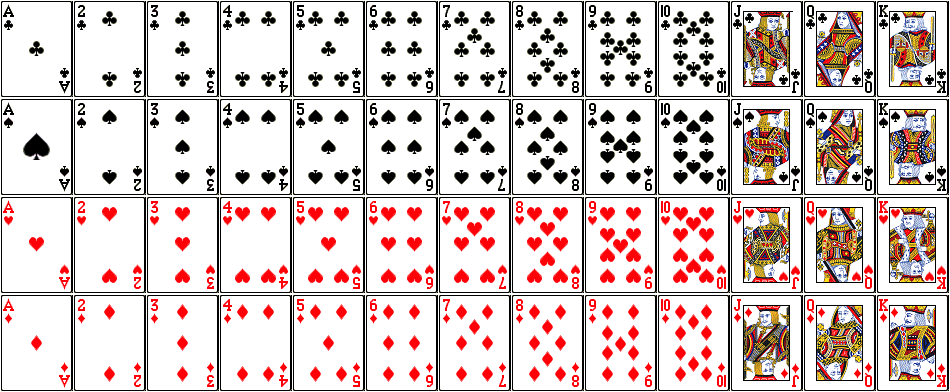
\includegraphics[width=\linewidth]{external/cards.png}
\end{image}%
\tcblower
\end{figureptx}%
\par\smallskip%
\noindent\textbf{\blocktitlefont Solution}.\hypertarget{ch-Probability-3-5-3}{}\quad{}There are 52 total outcomes in a standard deck.%
%
\begin{enumerate}
\item{}There are 4 aces in a deck. \(P(\text{ace}) = \frac{4}{52} = \frac{1}{13}\)%
\item{}There are 26 red cards (hearts and diamonds). \(P(\text{red}) = \frac{26}{52} = \frac{1}{2}\)%
\item{}There are 2 red kings (king of hearts and king of diamonds). \(P(\text{red king}) = \frac{2}{52} = \frac{1}{26}\)%
\item{}There are 13 spades in a deck. \(P(\text{spade}) = \frac{13}{52} = \frac{1}{4}\)%
\item{}The even numbered hearts are \(\{2, 4, 6, 8, 10\}\). There are 5 such cards. \(P(\text{even heart}) = \frac{5}{52}\)%
\item{}The odd numbered diamonds (excluding face cards) are \(\{3, 5, 7, 9\}\). (Note: Ace is usually not considered an odd number in this context, but if included, the count would be 5). Using \(\{3, 5, 7, 9\}\), there are 4 such cards. \(P(\text{odd diamond}) = \frac{4}{52} = \frac{1}{13}\)%
\item{}There are 12 face cards (Jack, Queen, King of each suit). \(P(\text{face card}) = \frac{12}{52} = \frac{3}{13}\)%
\end{enumerate}
\end{example}
\begin{example}{Example}{Probability of Three Coin Tosses.}{ch-Probability-3-6}%
A fair coin is tossed three times in succession. The set of equally likely outcomes is \(\{HHH, HHT, HTH, HTT, THH, THT, TTH, TTT\}\). Find the probability of getting:%
%
\begin{enumerate}
\item{}Exactly one tail.%
\item{}Exactly 2 heads.%
\item{}At least one head.%
\item{}Five tails.%
\end{enumerate}
\par\smallskip%
\noindent\textbf{\blocktitlefont Solution}.\hypertarget{ch-Probability-3-6-3}{}\quad{}\begin{figureptx}{Figure}{Tree diagram for three coin tosses}{fig-coin-toss-tree-clean}{}%
\begin{image}{0.05}{0.9}{0.05}{}%
\resizebox{\linewidth}{!}{%
\begin{tikzpicture}[
  grow=right,
  level 1/.style={sibling distance=8em, level distance=6em},
  level 2/.style={sibling distance=4em, level distance=6em},
  level 3/.style={sibling distance=2em, level distance=6em},
  edge from parent/.style={draw, -latex},
  every node/.style={circle, draw, minimum size=1.5em, inner sep=1pt}
]
\node {Start}
  child { node {T}
    child { node {T}
      child { node {T} }
      child { node {H} }
    }
    child { node {H}
      child { node {T} }
      child { node {H} }
    }
  }
  child { node {H}
    child { node {T}
      child { node {T} }
      child { node {H} }
    }
    child { node {H}
      child { node {T} }
      child { node {H} }
    }
  };
\end{tikzpicture}%
}%
\end{image}%
\tcblower
\end{figureptx}%
The total number of outcomes is 8.%
%
\begin{enumerate}
\item{}The outcomes with exactly one tail are \(\{HHT, HTH, THH\}\). There are 3 such outcomes, so \(P(\text{exactly one tail}) = \frac{3}{8}\).%
\item{}The outcomes with exactly two heads are \(\{HHT, HTH, THH\}\). There are 3 such outcomes, so \(P(\text{exactly 2 heads}) = \frac{3}{8}\).%
\item{}The only outcome with no heads is \(\{TTT\}\). Therefore, there are \(8 - 1 = 7\) outcomes with at least one head. \(P(\text{at least one head}) = \frac{7}{8}\).%
\item{}It is impossible to get five tails in only three tosses. \(P(\text{five tails}) = \frac{0}{8} = 0\).%
\end{enumerate}
\end{example}
\begin{inlineexercise}{Checkpoint}{Probability of a Coin Toss and Die Roll.}{ch-Probability-3-7}%
A coin is tossed and a die is rolled. The tree diagram below illustrates the sample space of 12 equally likely outcomes.%
\begin{figureptx}{Figure}{Tree diagram for tossing a coin and rolling a die.}{fig-tree-coin-die}{}%
\begin{image}{0.1}{0.8}{0.1}{}%
\resizebox{\linewidth}{!}{%
\begin{tikzpicture}[
  grow=right,
  level 1/.style={sibling distance=6cm, level distance=3cm},
  level 2/.style={sibling distance=1cm, level distance=3cm},
  edge from parent/.style={draw, -latex}]
  \node {}
    child {node {Tail}
      child {node {6} node[right=0.5cm] {(T, 6)}}
      child {node {5} node[right=0.5cm] {(T, 5)}}
      child {node {4} node[right=0.5cm] {(T, 4)}}
      child {node {3} node[right=0.5cm] {(T, 3)}}
      child {node {2} node[right=0.5cm] {(T, 2)}}
      child {node {1} node[right=0.5cm] {(T, 1)}}
    }
    child {node {Head}
      child {node {6} node[right=0.5cm] {(H, 6)}}
      child {node {5} node[right=0.5cm] {(H, 5)}}
      child {node {4} node[right=0.5cm] {(H, 4)}}
      child {node {3} node[right=0.5cm] {(H, 3)}}
      child {node {2} node[right=0.5cm] {(H, 2)}}
      child {node {1} node[right=0.5cm] {(H, 1)}}
    };
\end{tikzpicture}%
}%
\end{image}%
\tcblower
\end{figureptx}%
Find the probability of getting:%
%
\begin{enumerate}
\item{}a head and an even number.%
\item{}a tail and a number less than 3.%
\item{}a head and a number greater than 6.%
\end{enumerate}
\par\smallskip%
\noindent\textbf{\blocktitlefont Solution}.\hypertarget{ch-Probability-3-7-3}{}\quad{}The total number of equally likely outcomes is \(2 \times 6 = 12\).%
%
\begin{enumerate}
\item{}The outcomes for a head and an even number are \(\{(H, 2), (H, 4), (H, 6)\}\). There are 3 such outcomes, so \(P(\text{head and even}) = \frac{3}{12} = \frac{1}{4}\).%
\item{}The outcomes for a tail and a number less than 3 are \(\{(T, 1), (T, 2)\}\). There are 2 such outcomes, so \(P(\text{tail and less than 3}) = \frac{2}{12} = \frac{1}{6}\).%
\item{}Since a standard die only goes up to 6, it is impossible to roll a number greater than 6. The probability is \(\frac{0}{12} = 0\).%
\end{enumerate}
\end{inlineexercise}%
\end{sectionptx}
%
%
\typeout{************************************************}
\typeout{Section  3.2 Events Involving NOT and OR}
\typeout{************************************************}
%
\begin{sectionptx}{Section}{3.2 Events Involving NOT and OR}{}{3.2 Events Involving NOT and OR}{}{}{sec-events-not-or}
A survey asked 500 Americans to rate their health. Of the surveyed, 270 rated their health as good\slash{}excellent. This means that \(500 - 270 = 230\) people surveyed did not rate their health as good\slash{}excellent.%
\begin{align*}
P(\text{good/excellent}) + P(\text{not good/excellent}) \amp = \frac{270}{500} + \frac{230}{500}\\
\amp = \frac{500}{500} = 1
\end{align*}
In general, since the sum of probabilities of all possible outcomes in any situation is 1:%
\begin{equation*}
P(E) + P(\text{not } E) = 1
\end{equation*}
%
\begin{definition}{Definition}{The Probability of an Event Not Occurring.}{def-Not-probability}%
The probability that an event \(E\) will not occur is equal to 1 minus the probability that it will occur:%
\begin{equation*}
P(\text{not } E) = 1 - P(E)
\end{equation*}
%
\end{definition}
\begin{example}{Example}{}{sec-events-not-or-4}%
If you are dealt one card from a standard 52-card deck (\hyperref[fig-deck-of-cards]{Figure~{\xreffont\ref{fig-deck-of-cards}}}), find the probability that you are not dealt a queen.%
\par\smallskip%
\noindent\textbf{\blocktitlefont Solution}.\hypertarget{sec-events-not-or-4-2}{}\quad{}\(P(\text{not a queen}) = 1 - P(\text{queen}) = 1 - \frac{4}{52} = \frac{48}{52} = \frac{12}{13}\).%
\end{example}
\begin{inlineexercise}{Checkpoint}{}{sec-events-not-or-5}%
If you are dealt one card from a standard 52-card deck, find the probability that you are not dealt a diamond.%
\par\smallskip%
\noindent\textbf{\blocktitlefont Solution}.\hypertarget{sec-events-not-or-5-2}{}\quad{}\(P(\text{not a diamond}) = 1 - P(\text{diamond}) = 1 - \frac{13}{52} = \frac{39}{52} = \frac{3}{4}\).%
\end{inlineexercise}%
\begin{definition}{Definition}{Mutually Exclusive Events.}{def-mutually-exclusive}%
Two events are \alert{mutually exclusive} if they cannot occur at the same time. In other words, if one event occurs, the other cannot occur.%
\par
Or Probabilities with Mutually Exclusive Events: If \(A\) and \(B\) are mutually exclusive events, then:%
\begin{equation*}
P(A \text{ or } B) = P(A) + P(B)
\end{equation*}
%
\end{definition}
\begin{example}{Example}{}{sec-events-not-or-7}%
If one card is randomly selected from a deck of cards (\hyperref[fig-deck-of-cards]{Figure~{\xreffont\ref{fig-deck-of-cards}}}), what is the probability of selecting a king or a queen?%
\par\smallskip%
\noindent\textbf{\blocktitlefont Solution}.\hypertarget{sec-events-not-or-7-2}{}\quad{}These are mutually exclusive. \(P(\text{king or queen}) = \frac{4}{52} + \frac{4}{52} = \frac{8}{52} = \frac{2}{13}\).%
\end{example}
\begin{inlineexercise}{Checkpoint}{}{sec-events-not-or-8}%
If you roll a single, six-sided die, what is the probability of getting either a 4 or a 5?%
\par\smallskip%
\noindent\textbf{\blocktitlefont Solution}.\hypertarget{sec-events-not-or-8-2}{}\quad{}\(P(4 \text{ or } 5) = \frac{1}{6} + \frac{1}{6} = \frac{2}{6} = \frac{1}{3}\).%
\end{inlineexercise}%
If one card is randomly selected from a deck of cards (\hyperref[fig-deck-of-cards]{Figure~{\xreffont\ref{fig-deck-of-cards}}}), what is the probability of selecting a diamond or a picture card?%
\begin{equation*}
P(\text{diamond or picture card}) = P(\text{diamond}) + P(\text{picture card}) = \frac{13}{52} + \frac{12}{52}
\end{equation*}
However, there are three cards that are \alert{simultaneously diamonds and picture cards}. The events are not mutually exclusive.%
\par
To correct for the double-counting:%
\begin{align*}
P(\text{diamond or picture card}) \amp = P(\text{diamond}) + P(\text{picture card}) - P(\text{diamond and picture card})\\
\amp = \frac{13}{52} + \frac{12}{52} - \frac{3}{52} = \frac{22}{52} = \frac{11}{26}
\end{align*}
%
\begin{definition}{Definition}{Events that are NOT Mutually Exclusive.}{def-not-mutually-exclusive}%
If it is possible for events \(A\) and \(B\) to occur simultaneously, the events are said to be \alert{not mutually exclusive}.%
\par
If \(A\) and \(B\) are not mutually exclusive events, then:%
\begin{equation*}
P(A \text{ or } B) = P(A) + P(B) - P(A \text{ and } B)
\end{equation*}
%
\end{definition}
\begin{inlineexercise}{Checkpoint}{}{exercise-prob-math-psych}%
In a group of 50 students, 23 take math, 11 take psychology, and 7 take both. Find the probability that a randomly selected student takes math or psychology.%
\par\smallskip%
\noindent\textbf{\blocktitlefont Solution}.\hypertarget{exercise-prob-math-psych-2}{}\quad{}Let \(M\) be the event that a student takes math, and \(Ps\) be the event that a student takes psychology. We are given the following:%
\begin{itemize}[label=\ptxlistdisc]
\item{}Total students: \(n(S) = 50\)%
\item{}Students in math: \(n(M) = 23\)%
\item{}Students in psychology: \(n(Ps) = 11\)%
\item{}Students in both: \(n(M \text{ and } Ps) = 7\)%
\end{itemize}
%
\par
To find the probability that a student takes math \terminology{or} psychology, we use the Addition Rule for Probability:%
\begin{equation*}
P(M \text{ or } Ps) = P(M) + P(Ps) - P(M \text{ and } Ps)
\end{equation*}
%
\par
Substituting the known values as fractions of the total population:%
\begin{equation*}
P(M \text{ or } Ps) = \frac{23}{50} + \frac{11}{50} - \frac{7}{50}
\end{equation*}
%
\par
Since the denominators are the same, we combine the numerators:%
\begin{equation*}
\frac{23 + 11 - 7}{50} = \frac{27}{50}
\end{equation*}
%
\par
Thus, the probability that a randomly selected student takes math or psychology is \(\frac{27}{50}\) (or \(0.54\)).%
\end{inlineexercise}%
The following table shows the distribution of active duty personnel in the U.S. military (in thousands).%
\begin{tableptx}{Table}{\textbf{U.S. Military Personnel by Branch and Gender}}{table-military-personnel}{}%
\centering%
{\tabularfont%
\begin{tabular}{AcAcAcAcAcAcA}\hrulethin
{\bfseries{}}&{\bfseries{}Air Force}&{\bfseries{}Army}&{\bfseries{}Marine Corps}&{\bfseries{}Navy}&{\bfseries{}Total}\tabularnewline\hrulethin
Male&290&400&160&320&1,170\tabularnewline\hrulethin
Female&70&70&10&50&200\tabularnewline\hrulethin
Total&360&470&170&370&1,370\tabularnewline\hrulethin
\end{tabular}
}%
\end{tableptx}%
\begin{inlineexercise}{Checkpoint}{}{sec-events-not-or-15}%
Using \hyperref[table-military-personnel]{Table~{\xreffont\ref{table-military-personnel}}}, find the probability that a person selected at random is in the Army or is a woman.%
\par\smallskip%
\noindent\textbf{\blocktitlefont Solution}.\hypertarget{sec-events-not-or-15-2}{}\quad{}We use the Addition Rule for Probability:%
\begin{equation*}
P(\text{Army or Female}) = P(\text{Army}) + P(\text{Female}) - P(\text{Army and Female})
\end{equation*}
%
\par
From the table, we identify the following values:%
\begin{itemize}[label=\ptxlistdisc]
\item{}Total Personnel: \(1,370\)%
\item{}Total in Army: \(470\)%
\item{}Total Female: \(200\)%
\item{}Females in the Army (the overlap): \(70\)%
\end{itemize}
%
\par
Now, substitute these into the formula:%
\begin{equation*}
\frac{470}{1,370} + \frac{200}{1,370} - \frac{70}{1,370} = \frac{470 + 200 - 70}{1,370} = \frac{600}{1,370}
\end{equation*}
%
\par
Simplifying the fraction, we get \(\frac{60}{137} \approx 0.438\).%
\end{inlineexercise}%
\begin{inlineexercise}{Checkpoint}{}{sec-events-not-or-16}%
Using \hyperref[table-military-personnel]{Table~{\xreffont\ref{table-military-personnel}}}, find the probability that a person selected at random is in the Navy or is a man.%
\par\smallskip%
\noindent\textbf{\blocktitlefont Solution}.\hypertarget{sec-events-not-or-16-2}{}\quad{}To find the probability of a person being in the Navy or a man, we apply the Addition Rule:%
\begin{equation*}
P(\text{Navy or Male}) = P(\text{Navy}) + P(\text{Male}) - P(\text{Navy and Male})
\end{equation*}
%
\par
Identify the relevant values from the table:%
\begin{itemize}[label=\ptxlistdisc]
\item{}Total Personnel: \(1,370\)%
\item{}Total in Navy: \(370\)%
\item{}Total Male: \(1,170\)%
\item{}Males in the Navy (the overlap): \(320\)%
\end{itemize}
%
\par
Substitute the values:%
\begin{equation*}
\frac{370}{1,370} + \frac{1,170}{1,370} - \frac{320}{1,370} = \frac{370 + 1,170 - 320}{1,370} = \frac{1,220}{1,370}
\end{equation*}
%
\par
Simplifying the fraction, we get \(\frac{122}{137} \approx 0.891\).%
\end{inlineexercise}%
\end{sectionptx}
%
%
\typeout{************************************************}
\typeout{Section  3.3 The Fundamental Counting Principle}
\typeout{************************************************}
%
\begin{sectionptx}{Section}{3.3 The Fundamental Counting Principle}{}{3.3 The Fundamental Counting Principle}{}{}{notes-fcp}
\begin{introduction}{}%
The Fundamental Counting Principle is a powerful tool for counting the number of possible outcomes in a variety of situations. It allows us to determine the total number of combinations or arrangements by multiplying the number of choices for each independent event.%
\end{introduction}%
The probability of winning the top prize in the lottery is about the same as the probability of being struck by lightning. There are a million possible number combinations in the lottery games, and only one way of winning the grand prize.%
\par
We can generalize the idea to any two groups of items with the \alert{Fundamental Counting Principle}.%
\begin{definition}{Definition}{The Fundamental Counting Principle.}{definition-fundamental-counting-two-groups}%
If there are \(M\) ways to choose an item from one group and \(N\) ways to choose an item from another group, then there are \(M \cdot N\) ways to choose one item from each group.%
\end{definition}
\begin{example}{Example}{Restaurant two-course meal.}{example-two-course-meal-1}%
The Greasy Spoon Restaurant offers 6 appetizers and 14 main courses. In how many ways can a person order a two-course meal?%
\par\smallskip%
\noindent\textbf{\blocktitlefont Solution}.\hypertarget{example-two-course-meal-1-3}{}\quad{}Use the Fundamental Counting Principle: choose 1 appetizer and 1 main course.%
\(6 \cdot 14 = 84\)There are 84 different two-course meals.%
\end{example}
\begin{inlineexercise}{Checkpoint}{Two-course meal.}{exercise-two-course-meal}%
The Diner offers 10 appetizers and 15 main courses. In how many ways can a person order a two-course meal?%
\par\smallskip%
\noindent\textbf{\blocktitlefont Solution}.\hypertarget{exercise-two-course-meal-3}{}\quad{}Use the Fundamental Counting Principle and multiply the number of appetizers by the number of main courses.%
\(10 \cdot 15 = 150\)There are 150 possible two-course meals.%
\end{inlineexercise}%
\begin{inlineexercise}{Checkpoint}{Psychology and social science scheduling.}{exercise-course-schedule}%
This semester, you need to enroll in your required psychology and social science courses. Because you are registering early, you have 15 psychology sections to choose from. Additionally, there are 9 social science sections available that do not conflict with the psychology schedule. How many different two-course schedules can you create to fulfill these requirements?%
\par\smallskip%
\noindent\textbf{\blocktitlefont Solution}.\hypertarget{exercise-course-schedule-3}{}\quad{}Multiply the number of psychology section options by the number of social science section options.%
\(15 \cdot 9 = 135\)There are 135 possible two-course schedules.%
\end{inlineexercise}%
\begin{definition}{Definition}{The Fundamental Counting Principle.}{definition-fundamental-counting-multiple-events}%
If there are \(n\) independent events and the first event can occur in \(m_1\) ways, the second event can occur in \(m_2\) ways, the third event can occur in \(m_3\) ways, and so on, then the total number of ways that the events can occur is given by%
%
\begin{equation*}
m_1 \cdot m_2 \cdot m_3 \cdots m_n
\end{equation*}
by \alert{multiplying} the number of ways each individual event can happen.%
\end{definition}
\begin{example}{Example}{One-topping pizza choices.}{example-one-topping-pizza}%
A pizza can be ordered with two choices of size (medium or large), three choices of crust (thin, thick or regular), and five choices of toppings (ground beef, sausage, pepperoni, bacon and mushrooms). How many different one-topping pizzas can be ordered?%
\par\smallskip%
\noindent\textbf{\blocktitlefont Solution}.\hypertarget{example-one-topping-pizza-3}{}\quad{}Multiply the number of size choices by the number of crust choices and the number of topping choices.%
\(2 \cdot 3 \cdot 5 = 30\)There are 30 different one-topping pizzas.%
\end{example}
\begin{example}{Example}{Three-wheel car options.}{example-three-wheel-car-options}%
Car manufacturers are now experimenting with lightweight three-wheel cars, designed for one person and considered ideal for city driving. Suppose you could order such a car with a choice of 9 possible colors, with or without air conditioning, electric or gas powered, and with or without an on-board computer. In how many ways can this car be ordered with regard to these options?%
\par\smallskip%
\noindent\textbf{\blocktitlefont Solution}.\hypertarget{example-three-wheel-car-options-3}{}\quad{}Multiply the number of choices for each independent feature.%
\(9 \cdot 2 \cdot 2 \cdot 2 = 72\)There are 72 possible car orders.%
\end{example}
\begin{inlineexercise}{Checkpoint}{Ordering a customizable car.}{exercise-car-ordering-with-gps}%
The car in Example \hyperref[example-three-wheel-car-options]{Example~{\xreffont\ref{example-three-wheel-car-options}}} is now available in 10 possible colors. The options involving air conditioning, power, and on-board computer still apply. Furthermore, the car is available with or without a global positioning system. In how many ways can this car be ordered in terms of these options?%
\par\smallskip%
\noindent\textbf{\blocktitlefont Solution}.\hypertarget{exercise-car-ordering-with-gps-3}{}\quad{}Multiply the number of choices for each independent option.%
\(10 \cdot 2 \cdot 2 \cdot 2 \cdot 2 = 160\)There are 160 possible car orders.%
\end{inlineexercise}%
\begin{example}{Example}{Ten-question multiple-choice test.}{example-ten-question-test}%
You are taking a multiple-choice test that has ten questions. Each of the questions has four answer choices, with one correct answer per question. If you select one of these four choices for each question and leave nothing blank, in how many ways can you answer the questions?%
\par\smallskip%
\noindent\textbf{\blocktitlefont Solution}.\hypertarget{example-ten-question-test-3}{}\quad{}This situation involves making choices with ten questions.%
%
\begin{gather*}
\text{Question 1 (4 choices)}\\
\text{Question 2}\\
\text{Question 3}\\
\cdots\\
\text{Question 10}
\end{gather*}
We use the Fundamental Counting Principle to find the number of ways that you can answer the questions on the test. Multiply the number of choices, 4, for each of the ten questions.%
\(4 \cdot 4 \cdot 4 \cdot 4 \cdot 4 \cdot 4 \cdot 4 \cdot 4 \cdot 4 \cdot 4 = 4^{10} = 1,048,576\)\end{example}
%
%
\typeout{************************************************}
\typeout{Exercises  Exercises for Practice}
\typeout{************************************************}
%
\begin{exercises-subsection-numberless}{Exercises}{Exercises for Practice}{}{Exercises for Practice}{}{}{exercises-FCP}
\begin{divisionexercise}{1}{Six-question multiple-choice test.}{}{exercise-six-question-test}%
You are taking a multiple-choice test that has six questions. Each of the questions has three answer choices, with one correct answer per question. If you select one of these three choices for each question and leave nothing blank, in how many ways can you answer the questions?%
\par\smallskip%
\noindent\textbf{\blocktitlefont Solution}.\hypertarget{exercise-six-question-test-3}{}\quad{}Multiply the number of choices for each question.%
\(3^6 = 729\)There are 729 possible answer sheets.%
\end{divisionexercise}%
\begin{divisionexercise}{2}{Telephone number possibilities.}{}{exercise-telephone-numbers}%
Telephone numbers in the United States begin with three-digit area codes followed by seven-digit local telephone numbers. Area codes and local telephone numbers cannot begin with 0 or 1. How many different telephone numbers are possible?%
\par\smallskip%
\noindent\textbf{\blocktitlefont Solution}.\hypertarget{exercise-telephone-numbers-3}{}\quad{}There are 8 choices for the first digit of the area code and 10 choices for each remaining area code digit. For the local number, the first digit also has 8 choices and each remaining digit has 10 choices.%
\(8 \cdot 10 \cdot 10 \cdot 8 \cdot 10^6 = 6,400,000,000\)There are 6,400,000,000 possible telephone numbers.%
\end{divisionexercise}%
\begin{divisionexercise}{3}{Pen choices.}{}{exercise-pen-choices}%
A popular type of pen comes in red, blue, or black ink. The writing tip varies from extra bold, bold, regular, fine, or micro. How many different choices of pens do you have with this type of pen?%
\par\smallskip%
\noindent\textbf{\blocktitlefont Solution}.\hypertarget{exercise-pen-choices-3}{}\quad{}Multiply the ink color choices by the tip style choices.%
\(3 \cdot 5 = 15\)There are 15 different pen choices.%
\end{divisionexercise}%
\begin{divisionexercise}{4}{Catered meal combinations.}{}{exercise-catered-meal-combinations}%
A wedding caterer gives you three choices for the main course, six starter choices and five options for dessert. How many different meals (made up of starter, dinner and dessert) are there?%
\par\smallskip%
\noindent\textbf{\blocktitlefont Solution}.\hypertarget{exercise-catered-meal-combinations-3}{}\quad{}Multiply the number of starter choices, main course choices, and dessert choices.%
\(3 \cdot 6 \cdot 5 = 90\)There are 90 different meals.%
\end{divisionexercise}%
\begin{divisionexercise}{5}{Yes\slash{}no survey.}{}{exercise-yes-no-survey}%
You take a survey with five "yes" or "no" answers. How many different ways could you complete the survey?%
\par\smallskip%
\noindent\textbf{\blocktitlefont Solution}.\hypertarget{exercise-yes-no-survey-3}{}\quad{}Each question has 2 choices, and the choices are independent.%
\(2^5 = 32\)There are 32 different ways to complete the survey.%
\end{divisionexercise}%
\begin{divisionexercise}{6}{Product code possibilities.}{}{exercise-product-code-possibilities}%
A company puts a code on each different product they sell. The code is made up of 3 numbers and 2 letters. How many different codes are possible?%
\par\smallskip%
\noindent\textbf{\blocktitlefont Solution}.\hypertarget{exercise-product-code-possibilities-3}{}\quad{}Each number can be one of 10 digits, and each letter can be one of 26 letters.%
\(10^3 \cdot 26^2 = 676,000\)There are 676,000 different product codes possible.%
\end{divisionexercise}%
\end{exercises-subsection-numberless}
\end{sectionptx}
%
%
\typeout{************************************************}
\typeout{Section  3.4 Factorials}
\typeout{************************************************}
%
\begin{sectionptx}{Section}{3.4 Factorials}{}{3.4 Factorials}{}{}{notes-factorials}
\begin{introduction}{}%
In this section, we will explore the concept of factorials and how they are used in combinatorial counting problems. Factorials are a fundamental tool in counting arrangements and selections, and they play a crucial role in the formulas for permutations and combinations. We will define what a factorial is, how to compute it, and how to apply it in various counting scenarios.%
\end{introduction}%
\begin{assemblage}{Assemblage}{Factorials.}{assemblage-factorials}%
Factorials are a fundamental concept in combinatorics and play a crucial role in counting problems. The factorial of a positive integer \(n\), denoted as \(n!\), is the product of all positive integers from \(n\) down to 1. For example, %
\begin{align*}
1! \amp = 1\\
2! \amp = 2 \cdot 1 = 2\\
3! \amp = 3 \cdot 2 \cdot 1 = 6\\
4! \amp = 4 \cdot 3 \cdot 2 \cdot 1 = 24\\
5! \amp = 5 \cdot 4 \cdot 3 \cdot 2 \cdot 1 = 120
\end{align*}
%
 By definition, \(0!\) is equal to 1.%
\par
Factorials are used in various counting problems, such as permutations and combinations, where we need to count the number of ways to arrange or select items. In the following sections, we will explore how factorials are applied in these contexts and how they can help us solve complex counting problems.%
\par
If \(n\) is a positive integer, then \(n!\) (\alert{\(n\) factorial}) is the product of all positive integers from \(n\) down through 1.%
By definition, \(0!\) is 1.%
\end{assemblage}
\begin{definition}{Definition}{Factorial formula.}{definition-factorial-expression}%
The factorial of \(n\) is%
%
\begin{equation*}
n! = n(n-1)(n-2)(n-3)\cdots(3)(2)(1)
\end{equation*}
And by definition, \(0! = 1\).%
\end{definition}
\begin{example}{Example}{Evaluate factorial expressions.}{example-evaluate-factorial-expressions}%
Evaluate the following factorial expressions without using the factorial key on your calculator.%
%
\begin{multicols}{2}
\begin{enumerate}
\item{}\(\displaystyle \frac{8!}{5!}\)%
\item{}\(\displaystyle \frac{21!}{24!}\)%
\item{}\(\displaystyle \frac{500!}{499!}\)%
\item{}\(\displaystyle \frac{11!}{7!}\)%
\item{}\(\displaystyle \frac{13!}{16!}\)%
\item{}\(\displaystyle \frac{99!}{100!}\)%
\item{}\(\displaystyle \frac{7!}{(5-1)!}\)%
\item{}\(\displaystyle \frac{7!}{3!(4-4)!}\)%
\end{enumerate}
\end{multicols}
\par\smallskip%
\noindent\textbf{\blocktitlefont Solution}.\hypertarget{example-evaluate-factorial-expressions-3}{}\quad{}%
\begin{enumerate}
\item{}Expand both factorials completely to show the common factors:%
\begin{equation*}
\frac{8!}{5!} = \frac{8 \cdot 7 \cdot 6 \cdot 5 \cdot 4 \cdot 3 \cdot 2 \cdot 1}{5 \cdot 4 \cdot 3 \cdot 2 \cdot 1}
\end{equation*}
After canceling the common factors \((5 \cdot 4 \cdot 3 \cdot 2 \cdot 1)\) from the top and bottom:%
\begin{equation*}
8 \cdot 7 \cdot 6 = 336
\end{equation*}
%
\item{}Since the denominator is larger, the remaining factors will be in the denominator:%
\begin{equation*}
\frac{21!}{24 \cdot 23 \cdot 22 \cdot 21!} = \frac{1}{24 \cdot 23 \cdot 22} = \frac{1}{12,144}
\end{equation*}
%
\item{}%
\begin{equation*}
\frac{500 \cdot 499!}{499!} = 500
\end{equation*}
%
\item{}Expand both factorials completely:%
\begin{equation*}
\frac{11!}{7!} = \frac{11 \cdot 10 \cdot 9 \cdot 8 \cdot 7 \cdot 6 \cdot 5 \cdot 4 \cdot 3 \cdot 2 \cdot 1}{7 \cdot 6 \cdot 5 \cdot 4 \cdot 3 \cdot 2 \cdot 1}
\end{equation*}
After canceling the common factors \((7 \cdot 6 \cdot 5 \cdot 4 \cdot 3 \cdot 2 \cdot 1)\):%
\begin{equation*}
11 \cdot 10 \cdot 9 \cdot 8 = 7,920
\end{equation*}
%
\item{}%
\begin{equation*}
\frac{13!}{16 \cdot 15 \cdot 14 \cdot 13!} = \frac{1}{16 \cdot 15 \cdot 14} = \frac{1}{3,360}
\end{equation*}
%
\item{}%
\begin{equation*}
\frac{99!}{100 \cdot 99!} = \frac{1}{100}
\end{equation*}
%
\item{}First, simplify the expression inside the parentheses:%
\begin{equation*}
\frac{7!}{(5-1)!} = \frac{7!}{4!} = \frac{7 \cdot 6 \cdot 5 \cdot 4!}{4!} = 7 \cdot 6 \cdot 5 = 210
\end{equation*}
%
\item{}Recall that \(0! = 1\):%
\begin{equation*}
\frac{7!}{3!(4-4)!} = \frac{7!}{3! \cdot 0!} = \frac{7 \cdot 6 \cdot 5 \cdot 4 \cdot 3!}{3! \cdot 1} = 7 \cdot 6 \cdot 5 \cdot 4 = 840
\end{equation*}
%
\end{enumerate}
\end{example}
\begin{definition}{Definition}{Permutations of duplicate items.}{definition-permutations-duplicate}%
The number of permutations of \(n\) items, where \(p\) items are identical, \(q\) items are identical, \(r\) items are identical, \(s\) items are identical, and so on, is given by%
%
\begin{equation*}
\displaystyle \frac{n!}{(p!\ q!\ r!\ s!\cdots)}
\end{equation*}
\end{definition}
\begin{example}{Example}{Arrange MISSISSIPPI.}{example-arrange-mississippi}%
In how many distinct ways can the letters of the word "MISSISSIPPI" be arranged?%
\par\smallskip%
\noindent\textbf{\blocktitlefont Solution}.\hypertarget{example-arrange-mississippi-3}{}\quad{}The word has 11 letters with 4 identical I's, 4 identical S's, and 2 identical P's.%
\(\frac{11!}{(4! 4! 2!)} = \frac{39,916,800}{(24 \cdot 24 \cdot 2)} = 34,650\)\end{example}
\begin{example}{Example}{Arrange BANANA.}{example-arrange-banana}%
In how many distinct ways can the letters of the word "BANANA" be arranged?%
\par\smallskip%
\noindent\textbf{\blocktitlefont Solution}.\hypertarget{example-arrange-banana-3}{}\quad{}The word has 6 letters with 3 identical A's and 2 identical N's.%
\(\frac{6!}{(3! 2!)} = \frac{720}{(6 \cdot 2)} = 60\)\end{example}
\begin{inlineexercise}{Checkpoint}{Arrange MASSACHUSETTS.}{exercise-arrange-massachusetts}%
In how many distinct ways can the letters of the word "MASSACHUSETTS" be arranged?%
\par\smallskip%
\noindent\textbf{\blocktitlefont Solution}.\hypertarget{exercise-arrange-massachusetts-3}{}\quad{}The word has 13 letters with 4 identical S's, 2 identical A's, and 2 identical T's.%
\(\frac{13!}{(4! 2! 2!)} = \frac{6,227,020,800}{(24 \cdot 2 \cdot 2)} = 64,864,800\)\end{inlineexercise}%
\begin{inlineexercise}{Checkpoint}{Arrange balloons.}{exercise-arrange-balloons}%
There are seventeen balloons: 3 blue, 5 red, 2 green, 3 yellow, and 4 orange. In how many distinct ways can the balloons be arranged?%
\par\smallskip%
\noindent\textbf{\blocktitlefont Solution}.\hypertarget{exercise-arrange-balloons-3}{}\quad{}There are 17 total balloons with duplicates in several colors.%
\(\frac{17!}{(3! 5! 2! 3! 4!)} = \frac{355,687,428,096,000}{(6 \cdot 120 \cdot 2 \cdot 6 \cdot 24)} = 1,715,313,600\)\end{inlineexercise}%
\end{sectionptx}
%
%
\typeout{************************************************}
\typeout{Section  3.5 Permutations}
\typeout{************************************************}
%
\begin{sectionptx}{Section}{3.5 Permutations}{}{3.5 Permutations}{}{}{sec-permutations}
\begin{definition}{Definition}{Permutation.}{def-permutation}%
A \terminology{permutation} is an ordered arrangement of items that occurs when:%
\begin{itemize}[label=\ptxlistdisc]
\item{}No item is used more than once.%
\item{}The order of arrangement makes a difference.%
\end{itemize}
%
\end{definition}
\begin{example}{Example}{The BTS Concert Permutation Problem.}{example-concert-lineup}%
Suppose BTS, Blackstreet Boys, NSYNC and TLC are given a no-contact concert series. You decide that BTS should be the last group to perform at the four-group concert. Given this decision, in how many ways can you put together the concert?%
\par\smallskip%
\noindent\textbf{\blocktitlefont Solution}.\hypertarget{example-concert-lineup-3}{}\quad{}You can choose any one of the three groups (Blackstreet Boys, NSYNC, or TLC) as the opening act. Once you have chosen the first group, you will then have two groups left to choose for the second performance. You will then have just one group left to choose for the third performance. There is also just one choice for the closing act: BTS.%
\begin{tableptx}{Table}{\textbf{Concert Performance Choices}}{example-concert-lineup-3-2}{}%
\centering%
{\tabularfont%
\begin{tabular}{cccc}
First Group to perform&Second Group to perform&Third Group to perform&Last Group to perform\tabularnewline\hrulethin
3 choices&2 choices&1 choice&1 choice\tabularnewline[0pt]
Blackstreet Boys, NSYNC, TLC&&&BTS
\end{tabular}
}%
\end{tableptx}%
We use the Fundamental Counting Principle to find the number of ways you can put together the concert. Multiply the choices:%
\begin{equation*}
3 \cdot 2 \cdot 1 \cdot 1 = 6
\end{equation*}
Thus, there are six different ways to arrange the concert if BTS is the final group to perform.%
\end{example}
\begin{example}{Example}{Arrange books on a shelf.}{sec-permutations-4}%
You need to arrange five books along a small shelf. How many different ways can you arrange the books, assuming that the order of the books makes a difference to you?%
\par\smallskip%
\noindent\textbf{\blocktitlefont Solution}.\hypertarget{sec-permutations-4-3}{}\quad{}There are 5 choices for the first position, 4 for the second, 3 for the third, 2 for the fourth, and 1 for the last. Using the Fundamental Counting Principle:%
\begin{equation*}
5 \cdot 4 \cdot 3 \cdot 2 \cdot 1 = 5! = 120
\end{equation*}
There are 120 different ways to arrange the books.%
\end{example}
\begin{inlineexercise}{Checkpoint}{}{sec-permutations-5}%
In how many different ways can a police department arrange eight suspects in a police lineup if each lineup contains all eight people?%
\par\smallskip%
\noindent\textbf{\blocktitlefont Solution}.\hypertarget{sec-permutations-5-2}{}\quad{}Since all 8 people are used and order matters, this is a permutation of 8 items taken 8 at a time:%
\begin{equation*}
{}_8 P_8 = 8! = 40,320
\end{equation*}
There are 40,320 different ways to arrange the lineup.%
\end{inlineexercise}%
\begin{inlineexercise}{Checkpoint}{}{sec-permutations-6}%
If five digits 1, 2, 3, 4, 5 are being given and a three-digit code has to be made from it if the repetition of digits is allowed then how many such codes can be formed?%
\par\smallskip%
\noindent\textbf{\blocktitlefont Solution}.\hypertarget{sec-permutations-6-2}{}\quad{}Because repetition is allowed, there are 5 choices for each of the three positions in the code:%
\begin{equation*}
5 \cdot 5 \cdot 5 = 5^3 = 125
\end{equation*}
There are 125 possible codes.%
\end{inlineexercise}%
\begin{example}{Example}{Baseball Batting Lineup.}{example-baseball-lineup}%
You are the coach of a 13-player baseball team and must set a 9-player batting lineup. Because different positions in the lineup carry different responsibilities, \alert{the order makes a difference}. For example, a strong hitter like \textquotedblleft{}Barry\textquotedblright{} in the clean-up spot ( fourth) drives in more runs than a home run later in the order. How many different ways can you arrange your 9 starters?%
\par\smallskip%
\noindent\textbf{\blocktitlefont Solution}.\hypertarget{example-baseball-lineup-4}{}\quad{}You have 13 players to choose from for the first person at bat. This leaves 12 players for the second position, 11 for the third, and so on, until the 9th position. The total number of batting orders is:%
\begin{equation*}
13 \cdot 12 \cdot 11 \cdot 10 \cdot 9 \cdot 8 \cdot 7 \cdot 6 \cdot 5 = 259,459,200
\end{equation*}
There are nearly 260 million possible batting orders for a team of 13 players.%
\par
We can derive a general formula for permutations by rewriting this calculation as a fraction of factorials:%
\begin{equation*}
\frac{13 \cdot 12 \cdot 11 \cdot 10 \cdot 9 \cdot 8 \cdot 7 \cdot 6 \cdot 5 \cdot (4 \cdot 3 \cdot 2 \cdot 1)}{4 \cdot 3 \cdot 2 \cdot 1} = 
\frac{13!}{4!} = \frac{13!}{(13-9)!}
\end{equation*}
%
\par
Using standard notation, we call this \textquotedblleft{}the number of permutations of 13 things taken 9 at a time,\textquotedblright{} written as:%
\begin{equation*}
{}_{13}P_9 = \frac{13!}{(13-9)!}
\end{equation*}
%
\end{example}
\begin{note}{Note}{Calculator Note: Using the TI-30XIIS.}{sec-permutations-8}%
\begin{figureptx}{Figure}{TI-30XIIS Calculator}{calculator-note}{}%
\begin{image}{0.25}{0.5}{0.25}{}%
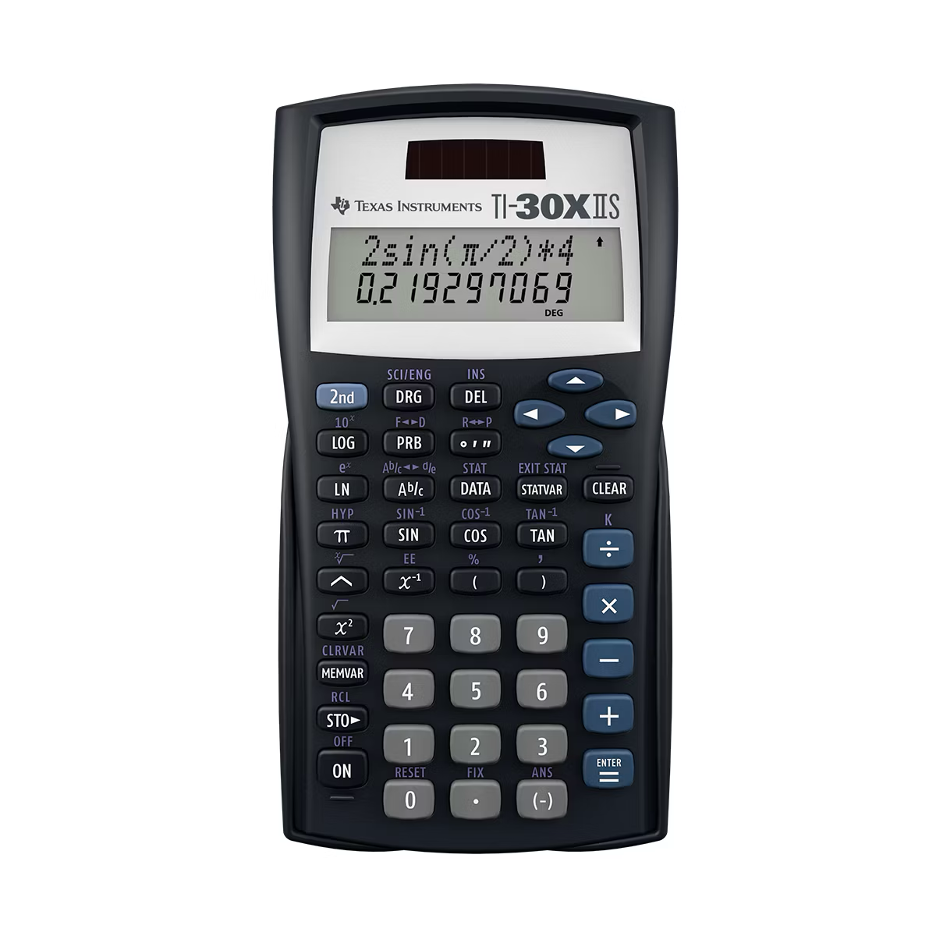
\includegraphics[width=\linewidth]{external/TI-30XIIS.png}
\end{image}%
\tcblower
\end{figureptx}%
%
\par
To evaluate \({}_{13}P_9\) on the TI-30XIIS, follow these steps:%
\begin{enumerate}
\item{}Enter the value of \(n\): Type \mono{13}.%
\item{}Press the \mono{PRB} key.%
\item{}The menu will display \mono{nPr} \mono{nCr} \mono{!}. Since \mono{nPr} is already underlined, simply press \mono{ENTER}.%
\item{}Enter the value of \(r\): Type \mono{9}.%
\item{}Press \mono{ENTER} to get the result: \mono{259,459,200}.%
\end{enumerate}
%
\end{note}
\begin{definition}{Definition}{Permutation Formula.}{def-permutation-formula}%
The notation \({}_n P_r\) means the \terminology{number of permutations of \(n\) things taken \(r\) at a time}:%
\begin{equation*}
{}_n P_r = \frac{n!}{(n-r)!}
\end{equation*}
%
\end{definition}
\begin{example}{Example}{Corporate Board Elections.}{example-board-elections}%
A corporation has seven members on its board of directors. In how many different ways can the board elect a president, vice-president, secretary, and treasurer?%
\par\smallskip%
\noindent\textbf{\blocktitlefont Solution}.\hypertarget{example-board-elections-3}{}\quad{}Since each officer holds a specific title, the order of selection matters. We are looking for the number of permutations of 7 items taken 4 at a time:%
\begin{equation*}
{}_{n}P_r = {}_{7}P_4 = \frac{7!}{(7-4)!} = \frac{7!}{3!}
\end{equation*}
Expanding the factorials, we get:%
\begin{equation*}
\frac{7 \cdot 6 \cdot 5 \cdot 4 \cdot 3 \cdot 2 \cdot 1}{3 \cdot 2 \cdot 1} = 7 \cdot 6 \cdot 5 \cdot 4 = 840
\end{equation*}
The board can elect the four officers in 840 different ways.%
\par
\alert{TI-30XIIS Keystrokes:} To calculate this on your TI-30XIIS: Type \mono{7} \(\rightarrow\) Press \mono{PRB} \(\rightarrow\) Select \mono{nPr} and press \mono{ENTER} \(\rightarrow\) Type \mono{4} \(\rightarrow\) Press \mono{ENTER}.%
\end{example}
\begin{inlineexercise}{Checkpoint}{}{sec-permutations-11}%
How many different programming schedules can be arranged by choosing 5 situation comedies from a collection of 9 classic sitcoms?%
\par\smallskip%
\noindent\textbf{\blocktitlefont Solution}.\hypertarget{sec-permutations-11-2}{}\quad{}We are choosing \(r=5\) items from a set of \(n=9\) where order matters:%
\begin{equation*}
{}_9 P_5 = \frac{9!}{(9-5)!} = \frac{9!}{4!} = 9 \cdot 8 \cdot 7 \cdot 6 \cdot 5 = 15,120
\end{equation*}
There are 15,120 possible programming schedules.%
\par
\alert{TI-30XIIS Keystrokes:} To calculate this on your TI-30XIIS: Type \mono{9} \(\rightarrow\) Press \mono{PRB} \(\rightarrow\) Select \mono{nPr} and press \mono{ENTER} \(\rightarrow\) Type \mono{5} \(\rightarrow\) Press \mono{ENTER}.%
\end{inlineexercise}%
\begin{inlineexercise}{Checkpoint}{}{sec-permutations-12}%
In a race in which six automobiles are entered and there are no ties, in how many ways can the first three finishers come in?%
\par\smallskip%
\noindent\textbf{\blocktitlefont Solution}.\hypertarget{sec-permutations-12-2}{}\quad{}We are looking for the number of permutations of 6 cars taken 3 at a time:%
\begin{equation*}
{}_6 P_3 = \frac{6!}{(6-3)!} = \frac{6!}{3!} = 6 \cdot 5 \cdot 4 = 120
\end{equation*}
There are 120 ways the first three finishers can come in.%
\end{inlineexercise}%
\begin{inlineexercise}{Checkpoint}{}{sec-permutations-13}%
Five singers are to perform on a weekend evening at a night club. How many different ways are there to schedule their appearances?%
\par\smallskip%
\noindent\textbf{\blocktitlefont Solution}.\hypertarget{sec-permutations-13-2}{}\quad{}This is a permutation of all 5 singers:%
\begin{equation*}
5! = 120
\end{equation*}
There are 120 different scheduling arrangements.%
\end{inlineexercise}%
\begin{inlineexercise}{Checkpoint}{}{sec-permutations-14}%
A stock can go up, go down, or stay unchanged. How many possibilities are there if you own seven stocks?%
\par\smallskip%
\noindent\textbf{\blocktitlefont Solution}.\hypertarget{sec-permutations-14-2}{}\quad{}Each of the 7 stocks has 3 possible outcomes. Since the outcome of one stock is independent of the others and order (which stock does what) matters:%
\begin{equation*}
3^7 = 2,187
\end{equation*}
There are 2,187 different possibilities for the seven stocks.%
\end{inlineexercise}%
\begin{inlineexercise}{Checkpoint}{}{sec-permutations-15}%
Seven seats are positioned in a row at a movie theater. Alice, Betty, Craig, Dan, Evelyn, Frank, and Gavin want to sit together.%
%
\begin{enumerate}
\item{}How many different ways can they be arranged?%
\item{}How many different ways can they be arranged if Betty sits in the second seat?%
\item{}How many different ways can they be arranged if Craig and Gavin want to sit in the two aisle seats?%
\end{enumerate}
\par\smallskip%
\noindent\textbf{\blocktitlefont Solution}.\hypertarget{sec-permutations-15-2}{}\quad{}%
\begin{enumerate}
\item{}Total arrangements of 7 people: \(7! = 5,040\).%
\item{}If Betty is fixed in the second seat, we only need to arrange the remaining 6 people in the remaining 6 seats: \(6! = 720\).%
\item{}There are two aisle seats (the first and the last). First, arrange Craig and Gavin in those 2 seats: \(2! = 2\) ways (Craig-Gavin or Gavin-Craig). Then, arrange the remaining 5 people in the middle 5 seats: \(5! = 120\). Total: \(2 \cdot 120 = 240\).%
\end{enumerate}
%
\end{inlineexercise}%
\end{sectionptx}
%
%
\typeout{************************************************}
\typeout{Section  3.6 Combinations}
\typeout{************************************************}
%
\begin{sectionptx}{Section}{3.6 Combinations}{}{3.6 Combinations}{}{}{sec-combinations}
\begin{definition}{Definition}{Combination.}{def-combination}%
A \terminology{combination} of items occurs when:%
\begin{itemize}[label=\ptxlistdisc]
\item{}The items are selected from the same group.%
\item{}No item is used more than once.%
\item{}\alert{The order of items makes no difference}.%
\end{itemize}
%
\end{definition}
\begin{inlineexercise}{Checkpoint}{Identifying Permutations and Combinations.}{ex-distinguish-perm-combo}%
For each of the following, determine whether the problem involves permutations or combinations:%
%
\begin{enumerate}
\item{}How many ways can you select 6 free videos from a list of 200 videos?%
\item{}In a race with 50 runners and no ties, in how many ways can the first three finishers come in?%
\item{}Baskin-Robbins offers 31 different flavors of ice cream. One item is a bowl consisting of three scoops, each a different flavor. How many such bowls are possible?%
\item{}A three-person committee is needed to study the possibility of expanding the neighborhood park. How many different committees could be formed from six people?%
\end{enumerate}
\par\smallskip%
\noindent\textbf{\blocktitlefont Solution}.\hypertarget{ex-distinguish-perm-combo-3}{}\quad{}%
\begin{enumerate}
\item{}\terminology{Combination}: the order of the selected videos does not matter; only which 6 are chosen matters.%
\item{}\terminology{Permutation}: first, second, and third place are distinct positions, so order matters.%
\item{}\terminology{Combination}: the bowl is defined by the set of three flavors, and swapping flavors produces the same bowl.%
\item{}\terminology{Combination}: the committee members are chosen without ordered roles.%
\end{enumerate}
%
\end{inlineexercise}%
\begin{definition}{Definition}{The Combination Formula.}{def-combination-formula}%
The number of combinations of \(n\) things taken \(r\) at a time is denoted by \({}_n C_r\):%
\par
%
\begin{equation*}
{}_n C_r = \frac{n!}{(n-r)! \, r!}
\end{equation*}
%
\end{definition}
\begin{example}{Example}{Public Transportation Committee.}{ex-committee-8}%
A three-person committee is needed to study ways of improving public transportation. How many committees could be formed from the eight people on the board of supervisors?%
\par\smallskip%
\noindent\textbf{\blocktitlefont Solution}.\hypertarget{ex-committee-8-3}{}\quad{}This is a combination because the order of committee members does not matter.%
\par
Compute%
\begin{equation*}
{}_8 C_3 = \frac{8!}{5!3!}\text{.}
\end{equation*}
%
\par
Simplify:%
\begin{equation*}
\frac{8 \cdot 7 \cdot 6 \cdot 5!}{5! \cdot (3 \cdot 2 \cdot 1)} = \frac{336}{6} = 56.
\end{equation*}
%
\par
There are 56 possible committees.%
\par
\alert{TI-30XIIS Keystrokes:} To calculate this on your TI-30XIIS: Type \mono{8} \(\rightarrow\) Press \mono{PRB} , use the arrow keys to underline \mono{nCr}, press \mono{ENTER} \(\rightarrow\) Type \mono{3} \(\rightarrow\) Press \mono{ENTER} again to get the result of 56.%
\end{example}
\begin{example}{Example}{Pet Combinations.}{ex-pet-sitting}%
You are volunteering to pet-sit for a friend who has seven different animals. How many different pet combinations are possible if you take three of the seven pets?%
\par\smallskip%
\noindent\textbf{\blocktitlefont Solution}.\hypertarget{ex-pet-sitting-3}{}\quad{}Order does not matter when choosing pets for a group, so use combinations.%
\par
%
\begin{equation*}
{}_7 C_3 = \frac{7!}{4!3!} = \frac{7 \cdot 6 \cdot 5}{3 \cdot 2 \cdot 1} = 35.
\end{equation*}
%
\par
\alert{TI-30XIIS Keystrokes:} To calculate this on your TI-30XIIS: Type \mono{7} \(\rightarrow\) Press \mono{PRB} , use the arrow keys to underline \mono{nCr}, press \mono{ENTER} \(\rightarrow\) Type \mono{3} \(\rightarrow\) Press \mono{ENTER} again to get the result of 35.%
\end{example}
\begin{example}{Example}{Four-Card Hand.}{ex-4-card-hand}%
How many different 4-card hands can be dealt from a deck that has 16 different cards?%
\par\smallskip%
\noindent\textbf{\blocktitlefont Solution}.\hypertarget{ex-4-card-hand-3}{}\quad{}A hand is a combination because the order of the cards does not matter.%
\par
%
\begin{equation*}
{}_{16} C_4 = \frac{16!}{12!4!} = \frac{16 \cdot 15 \cdot 14 \cdot 13}{4 \cdot 3 \cdot 2 \cdot 1} = 1,820.
\end{equation*}
%
\end{example}
\begin{example}{Example}{Poker Hands.}{ex-poker-hand}%
In poker, a person is dealt 5 cards from a standard 52-card deck (\hyperref[fig-deck-of-cards]{Figure~{\xreffont\ref{fig-deck-of-cards}}}). The order in which the cards are dealt does not matter. How many different 5-card poker hands are possible?%
\par\smallskip%
\noindent\textbf{\blocktitlefont Solution}.\hypertarget{ex-poker-hand-3}{}\quad{}Use combinations because only the set of cards matters.%
\par
%
\begin{equation*}
{}_{52} C_5 = \frac{52!}{47!5!} = 2,598,960.
\end{equation*}
%
\par
\alert{TI-30XIIS Keystrokes:} To calculate this on your TI-30XIIS: Type \mono{52} \(\rightarrow\) Press \mono{PRB} , use the arrow keys to underline \mono{nCr}, press \mono{ENTER} \(\rightarrow\) Type \mono{5} \(\rightarrow\) Press \mono{ENTER} again to get the result of 2,598,960.%
\end{example}
\begin{example}{Example}{Senate Committee Selection.}{ex-107-congress}%
The U.S. Senate of the 107th Congress consisted of 50 Democrats, 49 Republicans, and one independent. How many committees can be formed if each committee must have 3 Democrats and 2 Republicans?%
\par\smallskip%
\noindent\textbf{\blocktitlefont Solution}.\hypertarget{ex-107-congress-3}{}\quad{}Use combinations because the order of committee members does not matter.%
\par
Choose 3 Democrats from 50:%
\begin{equation*}
{}_{50} C_3 = 19,600\text{.}
\end{equation*}
%
\par
Choose 2 Republicans from 49:%
\begin{equation*}
{}_{49} C_2 = 1,176\text{.}
\end{equation*}
%
\par
Total committees:%
\begin{equation*}
19,600 \times 1,176 = 23,049,600.
\end{equation*}
%
\par
\alert{TI-30XIIS Keystrokes:} To calculate \({}_{50} C_3\): Type \kbd{50} \(\rightarrow\) Press \kbd{PRB}, use the arrow keys to underline \mono{nCr}, press \kbd{ENTER} \(\rightarrow\) Type \kbd{3} \(\rightarrow\) Press \kbd{ENTER}. Repeat the process for \({}_{49} C_2\) and multiply the results.%
\end{example}
\begin{inlineexercise}{Checkpoint}{Practice Problems.}{ex-practice-combination-counting}%
Answer the following problems. Identify whether each situation uses combinations, permutations, or the product rule, and then compute the requested count.%
%
\begin{enumerate}
\item{}A popular brand of pen is available in three colors and four writing tips. How many different choices of pens do you have with this brand?%
\item{}How many four-digit odd numbers are there?%
\item{}An election ballot asks voters to select three city commissioners from a group of eight candidates. In how many ways can this be done?%
\item{}Six singers are to perform on a weekend evening at a nightclub. How many different ways are there to schedule their appearances?%
\item{}In how many ways can you arrange six books along a shelf, assuming that the order of the books makes a difference?%
\item{}An ice cream store sells two drinks in four sizes and five flavors. In how many ways can a customer order a drink?%
\item{}An electronic gate can be opened by entering five digits on a keypad containing the digits 0–9. How many different keypad sequences are possible if the digit 0 cannot be used as the first digit?%
\item{}A math exam consists of 10 multiple-choice questions and 5 open-ended problems in which all work must be shown. If a student must answer 8 of the multiple-choice questions and 3 of the open-ended problems, in how many ways can the questions and problems be chosen?%
\item{}For a temporary job, you are painting parking spaces for a new shopping mall with a letter of the alphabet and a single digit from 1 to 9. The first parking space is A1 and the last parking space is Z9. How many parking spaces can you paint with distinct labels?%
\item{}In a race with 100 runners and no ties, in how many ways can the first three finishers come in?%
\item{}Six people are on the board of supervisors for your neighborhood park. A three-person committee is needed to study the possibility of expanding the park. How many different committees could be formed from the six people?%
\item{}Nine comedy acts will perform over two evenings. Five of the acts will perform on the first evening. How many ways can the schedule for the first evening be made?%
\item{}To win Mega Millions, you must pick 5 numbers from a collection of 56 and one Megaball number from a collection of 46. The order of the first 5 does not matter. How many different selections are possible?%
\item{}An exam consists of 20 multiple-choice questions and 10 open-ended problems. If a student must answer 15 of the multiple-choice and 5 of the open-ended questions, in how many ways can the questions and problems be chosen?%
\item{}In a lucky draw, 10 names are placed in a box and three are drawn. Find the number of ways those three names can be selected.%
\end{enumerate}
\par\smallskip%
\noindent\textbf{\blocktitlefont Solution}.\hypertarget{ex-practice-combination-counting-3}{}\quad{}%
\begin{enumerate}
\item{}Since we are making two independent choices (brand and color), we use the \terminology{Product Rule}. Multiply the number of brand options by the number of color options:%
\begin{equation*}
3 \times 4 = 12 \text{ different pen choices.}
\end{equation*}
%
\item{}We use the \terminology{Fundamental Counting Principle} for each of the four digits:%
\begin{itemize}[label=\ptxlistdisc]
\item{}First digit (1-9): 9 choices%
\item{}Middle digits (0-9): 10 choices each%
\item{}Last digit (odd): 5 choices (1, 3, 5, 7, 9)%
\end{itemize}
%
\begin{equation*}
9 \times 10 \times 10 \times 5 = 4,500 \text{ possible codes.}
\end{equation*}
%
\item{}This is a \terminology{combination} because the order of committee members does not matter.%
\begin{equation*}
{}_8 C_3 = \frac{8!}{3!(8-3)!} = \frac{8 \cdot 7 \cdot 6}{3 \cdot 2 \cdot 1} = 56.
\end{equation*}
%
\item{}This is a \terminology{permutation} of all 6 distinct subjects.%
\begin{equation*}
6! = 6 \cdot 5 \cdot 4 \cdot 3 \cdot 2 \cdot 1 = 720 \text{ possible schedules.}
\end{equation*}
%
\item{}Arranging all items in a row is a \terminology{permutation}.%
\begin{equation*}
6! = 720 \text{ arrangements.}
\end{equation*}
%
\item{}By the \terminology{Product Rule}, multiply the choices for size, caffeine, and flavor:%
\begin{equation*}
2 \times 4 \times 5 = 40 \text{ possible drink orders.}
\end{equation*}
%
\item{}The first digit cannot be zero (9 choices), and the remaining four digits can be any number 0-9 (10 choices each):%
\begin{equation*}
9 \times 10 \times 10 \times 10 \times 10= 9 \times 10^4 = 90{,}000 \text{ codes.}
\end{equation*}
%
\item{}Select the items separately then multiply:%
\begin{equation*}
{}_{10} C_8 = 45 \text{ and } {}_5 C_3 = 10
\end{equation*}
%
\begin{equation*}
45 \times 10 = 450 \text{ total combinations.}
\end{equation*}
%
\item{}Multiply the number of letter options by the number of digit options:%
\begin{equation*}
26 \times 9 = 234 \text{ possible outcomes.}
\end{equation*}
%
\item{}Since the positions (President, VP, Secretary) are distinct, order matters; this is a \terminology{permutation}.%
\begin{equation*}
{}_6 P_3 = 6 \times 5 \times 4 = 120.
\end{equation*}
%
\item{}Choosing a subgroup where order is irrelevant is a \terminology{combination}.%
\begin{equation*}
{}_6 C_3 = \frac{6 \times 5 \times 4}{3 \times 2 \times 1} = 20.
\end{equation*}
%
\item{}Select 5 players from 9 without regard to order:%
\begin{equation*}
{}_9 C_5 = \frac{9 \times 8 \times 7 \times 6}{4 \times 3 \times 2 \times 1} = 126.
\end{equation*}
%
\item{}First, calculate the combinations for the 5 white balls, then multiply by the Megaball choice:%
\begin{equation*}
{}_{56} C_5 = 3{,}819{,}816
\end{equation*}
%
\begin{equation*}
3{,}819{,}816 \times 46 = 175{,}711{,}536.
\end{equation*}
%
\item{}Calculate the ways to choose the two groups separately:%
\begin{equation*}
{}_{20} C_{15} = 15{,}504 \text{ and } {}_{10} C_5 = 252
\end{equation*}
%
\begin{equation*}
15{,}504 \times 252 = 3{,}907{,}008.
\end{equation*}
%
\item{}Selecting a group of 3 from 10 is a \terminology{combination}:%
\begin{equation*}
{}_{10} C_3 = \frac{10 \times 9 \times 8}{3 \times 2 \times 1} = 120.
\end{equation*}
%
\end{enumerate}
%
\end{inlineexercise}%
\end{sectionptx}
%
%
\typeout{************************************************}
\typeout{Section  3.7 Probability with the FCP, nPr and nCr}
\typeout{************************************************}
%
\begin{sectionptx}{Section}{3.7 Probability with the FCP, nPr and nCr}{}{3.7 Probability with the FCP, nPr and nCr}{}{}{sec-probability-fcp-npr-ncr}
%
%
\typeout{************************************************}
\typeout{Subsection  Probability with Fundamental Counting Principle and permutations, nPr}
\typeout{************************************************}
%
\begin{subsectionptx}{Subsection}{Probability with Fundamental Counting Principle and permutations, nPr}{}{Probability with Fundamental Counting Principle and permutations, nPr}{}{}{subsec-nPr-Probability}
\begin{introduction}{}%
We return to our concert series with BTS, Blackstreet Boys, NSYNC and TLC. Now, \terminology{New Kids on the Block (NKOTB)} agrees to join the tour. The five groups determine the performance order by drawing names from a hat.%
\par
What is the probability of \terminology{TLC} performing fourth and \terminology{BTS} performing last?%
\end{introduction}%
Recall the probability formula (\hyperref[def-theoretical-probability]{Definition~{\xreffont\ref{def-theoretical-probability}}}), the probability is the fraction of the number of event outcomes over the total number of possible outcomes.%
\par
To solve this problem, we will use the \terminology{Fundamental Counting Principle (FCP)} to find the total number of possible arrangements of the five groups, and then determine how many of those arrangements have TLC performing fourth and BTS performing last.%
\noindent\hypertarget{subsec-nPr-Probability-5-main}{}\textbraceleft{}\textbraceright{}The probability is defined as:%
\begin{equation*}
P(\text{TLC 4th, BTS last}) = \frac{\text{number of permutations with TLC 4th, BTS last}}{\text{total number of possible permutations}}
\end{equation*}
%
\par
First, we find the total number of ways to arrange the 5 groups using the \terminology{Fundamental Counting Principle}:%
\begin{equation*}
5 \cdot 4 \cdot 3 \cdot 2 \cdot 1 = 120
\end{equation*}
%
\par
Next, we find the number of successful outcomes where TLC is 4th and BTS is last. By fixing these two positions, we only need to arrange the remaining 3 groups (Backstreet Boys, NSYNC, and NKOTB) in the first three slots:%
\begin{itemize}[label=\ptxlistdisc]
\item{}1st spot: 3 choices%
\item{}2nd spot: 2 choices%
\item{}3rd spot: 1 choice%
\item{}4th spot: \alert{Fixed (TLC)}%
\item{}5th spot: \alert{Fixed (BTS)}%
\end{itemize}
%
\begin{equation*}
3 \cdot 2 \cdot 1 \cdot 1 \cdot 1 = 6
\end{equation*}
%
\par
Therefore, calculate the probability:%
\begin{equation*}
P(\text{TLC 4th, BTS last}) = \frac{6}{120} = \frac{1}{20}
\end{equation*}
%
\par
\alert{TI-30XIIS Keystrokes:} To find the total permutations (5!), type \kbd{5} \(\rightarrow\) \kbd{PRB} \(\rightarrow\) arrow over to underline \mono{!} \(\rightarrow\) \kbd{ENTER} \(\rightarrow\) \kbd{ENTER}. The result is 120.%
\begin{inlineexercise}{Checkpoint}{Probability of Performers.}{subsec-nPr-Probability-6}%
Seven performers A, B, C, D, E, F, and G are to appear in a fundraiser. The order of performance is determined by random selection. Find the probability that:%
\par
%
\begin{enumerate}[label={\alph*}]
\item{}D will perform first.%
\item{}E will perform sixth and B will perform last.%
\item{}They will perform in the following order: C, D, B, A, G, F, E.%
\item{}F or G will perform first.%
\end{enumerate}
%
\par\smallskip%
\noindent\textbf{\blocktitlefont Solution}.\hypertarget{subsec-nPr-Probability-6-3}{}\quad{}First, we find the \terminology{total number of possible outcomes} for the sample space. Since there are 7 positions to fill:%
\begin{equation*}
\underline{7} \times \underline{6} \times \underline{5} \times \underline{4} \times \underline{3} \times \underline{2} \times \underline{1}
\end{equation*}
%
\begin{equation*}
7! = 5{,}040
\end{equation*}
\alert{TI-30XIIS:} Type \kbd{7} \(\rightarrow\) Press \kbd{PRB} \(\rightarrow\) Arrow right to underline \mono{!} \(\rightarrow\) Press \kbd{ENTER} \(\rightarrow\) Press \kbd{ENTER}.%
%
\par
%
\begin{enumerate}[label={\alph*}]
\item{}To find the number of ways \alert{D can perform first}, we fix D in the first spot:%
\begin{equation*}
\underline{1 (D)} \times \underline{6} \times \underline{5} \times \underline{4} \times \underline{3} \times \underline{2} \times \underline{1} = 720
\end{equation*}
%
\begin{equation*}
P(\text{D first}) = \frac{720}{5,040} = \frac{1}{7}
\end{equation*}
%
\item{}To find the number of ways \alert{E performs 6th and B performs last}, we fix those two positions:%
\begin{equation*}
\underline{5} \times \underline{4} \times \underline{3} \times \underline{2} \times \underline{1} \times \underline{1 (E)} \times \underline{1 (B)} = 120
\end{equation*}
%
\begin{equation*}
P(\text{E 6th, B last}) = \frac{120}{5,040} = \frac{1}{42}
\end{equation*}
%
\item{}There is only \alert{one specific sequence} out of the 5,040 possibilities:%
\begin{equation*}
\underline{1 (C)} \times \underline{1 (D)} \times \underline{1 (B)} \times \underline{1 (A)} \times \underline{1 (G)} \times \underline{1 (F)} \times \underline{1 (E)} = 1
\end{equation*}
%
\begin{equation*}
P(\text{Specific order C, D, B, A, G, F, E}) = \frac{1}{5,040}
\end{equation*}
%
\item{}For \alert{F or G to perform first}, we have 2 choices for the first spot:%
\begin{equation*}
\underline{2 (\text{F or G})} \times \underline{6} \times \underline{5} \times \underline{4} \times \underline{3} \times \underline{2} \times \underline{1} = 1{,}440
\end{equation*}
%
\begin{equation*}
P(\text{F or G first}) = \frac{1,440}{5,040} = \frac{2}{7}
\end{equation*}
%
\end{enumerate}
%
\end{inlineexercise}%
\end{subsectionptx}
%
%
\typeout{************************************************}
\typeout{Subsection  Probability with Combinations, nCr}
\typeout{************************************************}
%
\begin{subsectionptx}{Subsection}{Probability with Combinations, nCr}{}{Probability with Combinations, nCr}{}{}{subsec-nCr-Probability}
\begin{example}{Example}{Probability of Winning LOTTO.}{subsec-nCr-Probability-2}%
Florida's lottery game LOTTO is set up so that each player chooses six different numbers from 1 to 53. If the six numbers chosen match the six numbers drawn randomly, the player wins the top cash prize. With one LOTTO ticket, what is the probability of winning this prize?%
\noindent\hypertarget{subsec-nCr-Probability-2-3}{}Because the order of the six numbers does not matter, this is a situation involving combinations. We begin with the formula for probability:%
\begin{equation*}
P(\text{winning}) = \frac{\text{number of ways of winning}}{\text{total number of possible combinations}}
\end{equation*}
%
\par
We are selecting \(r = 6\) numbers from a collection of \(n = 53\) numbers. Using the combination formula:%
\begin{equation*}
{}_{53}C_6 = \frac{53!}{(53 - 6)! \times 6!} = \frac{53!}{47! \times 6!} = 22{,}957{,}480
\end{equation*}
%
\par
\alert{TI-30XIIS Keystrokes:} To calculate \({}_{53}C_6\): Type \kbd{53} \(\rightarrow\) Press \kbd{PRB} \(\rightarrow\) Underline \mono{nCr} and press \kbd{ENTER} \(\rightarrow\) Type \kbd{6} \(\rightarrow\) Press \kbd{ENTER}.%
\par
There are nearly 23 million number combinations possible in LOTTO. If a person buys one LOTTO ticket, that person has selected only one combination of six numbers. With one LOTTO ticket, there is only one way of winning:%
\begin{equation*}
P(\text{winning}) = \frac{1}{22{,}957{,}480} \approx 0.0000000436
\end{equation*}
%
\par
The probability of winning the top prize with one LOTTO ticket is \(\frac{1}{22{,}957{,}480}\) or about 1 in 23 million.%
\end{example}
\begin{inlineexercise}{Checkpoint}{}{subsec-nCr-Probability-3}%
A state lottery is designed so that a player chooses five numbers from 1 to 30 on one lottery ticket. What is the probability that a player with one lottery ticket will win? What is the probability of winning if 100 different lottery tickets are purchased?%
\par\smallskip%
\noindent\textbf{\blocktitlefont Hint}.\hypertarget{subsec-nCr-Probability-3-3}{}\quad{}To calculate \({}_{30}C_{5}\) on your \terminology{TI-30XIIS}:%
\begin{enumerate}
\item{}Enter \kbd{30}.%
\item{}Press the \kbd{PRB} key.%
\item{}Use the \kbd{Right Arrow} to underline \terminology{nCr}.%
\item{}Press \kbd{ENTER}.%
\item{}Enter \kbd{5} and press \kbd{ENTER} (Result: 142,506).%
\item{}To find the probability, press \kbd{1} \kbd{÷} \kbd{2nd} \kbd{ANS} \kbd{ENTER}.%
\end{enumerate}
%
\par\smallskip%
\noindent\textbf{\blocktitlefont Solution}.\hypertarget{subsec-nCr-Probability-3-2}{}\quad{}The total number of possible outcomes is the number of ways to choose 5 numbers from 30:%
\begin{equation*}
{}_{30}C_{5} = 142,506
\end{equation*}
%
\par
The probability of winning with one ticket is:%
\begin{equation*}
P(\text{1 ticket}) = \frac{1}{142,506} \approx 0.000007
\end{equation*}
%
\par
The probability of winning with 100 tickets is:%
\begin{equation*}
P(\text{100 tickets}) = \frac{100}{142,506} \approx 0.0007
\end{equation*}
%
\end{inlineexercise}%
\begin{example}{Example}{Probability of Club Committee Selection.}{subsec-nCr-Probability-4}%
A club consists of five men and seven women. Three members are selected at random to attend a conference. Find the probability that the selected group consists of:%
\begin{enumerate}[label={\alph*}]
\item{}three men.%
\item{}one man and two women.%
\end{enumerate}
%
\par\smallskip%
\noindent\textbf{\blocktitlefont Solution}.\hypertarget{subsec-nCr-Probability-4-3}{}\quad{}First, we find the total number of ways to choose 3 members from the group of 12 (5 men + 7 women):%
\begin{equation*}
{}_{12}C_{3} = 220
\end{equation*}
%
\par
%
\begin{enumerate}[label={\alph*}]
\item{}To find the probability of selecting three men, we first find the number of ways to choose 3 men from the 5 available:%
\begin{equation*}
{}_{5}C_{3} = 10
\end{equation*}
%
\par
The probability is:%
\begin{equation*}
P(\text{3 men}) = \frac{{}_{5}C_{3}}{{}_{12}C_{3}} = \frac{10}{220} = \frac{1}{22} \approx 0.0455
\end{equation*}
%
\item{}To find the probability of selecting one man and two women, we calculate the ways to choose each and multiply them:%
\begin{itemize}[label=\ptxlistdisc]
\item{}Ways to choose 1 man from 5: \({}_{5}C_{1} = 5\)%
\item{}Ways to choose 2 women from 7: \({}_{7}C_{2} = 21\)%
\end{itemize}
%
\begin{equation*}
P(\text{1 man, 2 women}) = \frac{{}_{5}C_{1} \times {}_{7}C_{2}}{{}_{12}C_{3}} = \frac{5 \times 21}{220} = \frac{105}{220} = \frac{21}{44} \approx 0.4773
\end{equation*}
%
\end{enumerate}
%
\par
\terminology{TI-30XIIS Tip:} To calculate part (b) in one string: \kbd{5} \kbd{PRB} (\terminology{nCr}) \kbd{1} \kbd{×} \kbd{7} \kbd{PRB} (\terminology{nCr}) \kbd{2} \kbd{÷} \kbd{220} \kbd{ENTER}.%
\end{example}
\begin{inlineexercise}{Checkpoint}{Probability of Defective Transistors.}{subsec-nCr-Probability-5}%
A box contains 25 transistors, 6 of which are defective. If 6 are selected at random, find the probability that:%
\begin{enumerate}[label={\alph*}]
\item{}all are defective.%
\item{}none are defective.%
\end{enumerate}
%
\par\smallskip%
\noindent\textbf{\blocktitlefont Solution}.\hypertarget{subsec-nCr-Probability-5-3}{}\quad{}First, we determine the total number of ways to select 6 transistors from 25:%
\begin{equation*}
{}_{25}C_{6} = 177,100
\end{equation*}
%
\par
%
\begin{enumerate}[label={\alph*}]
\item{}To find the probability that all 6 are defective, we choose 6 from the 6 defective transistors:%
\begin{equation*}
{}_{6}C_{6} = 1
\end{equation*}
%
\begin{equation*}
P(\text{all defective}) = \frac{1}{177,100} \approx 0.0000056
\end{equation*}
%
\item{}To find the probability that none are defective, all 6 must be chosen from the 19 non-defective transistors (25 total - 6 defective):%
\begin{equation*}
{}_{19}C_{6} = 27,132
\end{equation*}
%
\begin{equation*}
P(\text{none defective}) = \frac{27,132}{177,100} = \frac{6,783}{44,275} \approx 0.1532
\end{equation*}
%
\end{enumerate}
%
\par
\terminology{TI-30XIIS Calculator Steps:}%
\begin{itemize}[label=\ptxlistdisc]
\item{}For the denominator: \kbd{25} \kbd{PRB} (\terminology{nCr}) \kbd{6} \kbd{ENTER} (Result: 177,100).%
\item{}For part (b): \kbd{19} \kbd{PRB} (\terminology{nCr}) \kbd{6} \kbd{÷} \kbd{177,100} \kbd{ENTER}.%
\end{itemize}
%
\end{inlineexercise}%
\begin{inlineexercise}{Checkpoint}{Parent-Teacher Committee Selection.}{subsec-nCr-Probability-6}%
A parent-teacher committee consisting of four people is to be selected from fifteen parents and five teachers. Find the probability of selecting two parents and two teachers.%
\par\smallskip%
\noindent\textbf{\blocktitlefont Solution}.\hypertarget{subsec-nCr-Probability-6-3}{}\quad{}First, we find the total number of ways to choose 4 members from the group of 20 (15 parents + 5 teachers):%
\begin{equation*}
{}_{20}C_{4} = 4,845
\end{equation*}
%
\par
Next, we find the number of ways to select the specific group:%
\begin{itemize}[label=\ptxlistdisc]
\item{}Ways to select 2 parents from 15: \({}_{15}C_{2} = 105\)%
\item{}Ways to select 2 teachers from 5: \({}_{5}C_{2} = 10\)%
\end{itemize}
Total successful outcomes: \(105 \times 10 = 1,050\).%
\par
The probability is the number of successful outcomes divided by the total outcomes:%
\begin{equation*}
P(\text{2 parents, 2 teachers}) = \frac{{}_{15}C_{2} \times {}_{5}C_{2}}{{}_{20}C_{4}} = \frac{1,050}{4,845}
\end{equation*}
%
\par
Simplifying the fraction and providing the decimal:%
\begin{equation*}
P = \frac{70}{323} \approx 0.2167
\end{equation*}
%
\par
\terminology{TI-30XIIS Calculator Steps:} \kbd{15} \kbd{PRB} (\terminology{nCr}) \kbd{2} \kbd{×} \kbd{5} \kbd{PRB} (\terminology{nCr}) \kbd{2} \kbd{÷} \kbd{20} \kbd{PRB} (\terminology{nCr}) \kbd{4} \kbd{ENTER}.%
\end{inlineexercise}%
\begin{inlineexercise}{Checkpoint}{Probability of Dealing Four Hearts.}{subsec-nCr-Probability-7}%
If you are dealt 4 cards from a shuffled deck of 52 cards (\hyperref[fig-deck-of-cards]{Figure~{\xreffont\ref{fig-deck-of-cards}}}), find the probability that all 4 are hearts.%
\par\smallskip%
\noindent\textbf{\blocktitlefont Solution}.\hypertarget{subsec-nCr-Probability-7-3}{}\quad{}First, we determine the total number of ways to choose 4 cards from a deck of 52:%
\begin{equation*}
{}_{52}C_{4} = 270,725
\end{equation*}
%
\par
Next, we determine the number of ways to choose 4 hearts. Since there are 13 hearts in a deck:%
\begin{equation*}
{}_{13}C_{4} = 715
\end{equation*}
%
\par
The probability that all 4 cards are hearts is the number of ways to choose 4 hearts divided by the total number of ways to choose 4 cards:%
\begin{equation*}
P(\text{4 hearts}) = \frac{{}_{13}C_{4}}{{}_{52}C_{4}} = \frac{715}{270,725}
\end{equation*}
%
\par
Simplifying the fraction and providing the decimal:%
\begin{equation*}
P = \frac{11}{4,165} \approx 0.0026
\end{equation*}
%
\par
\terminology{TI-30XIIS Calculator Steps:} \kbd{13} \kbd{PRB} (\terminology{nCr}) \kbd{4} \kbd{÷} \kbd{52} \kbd{PRB} (\terminology{nCr}) \kbd{4} \kbd{ENTER}.%
\end{inlineexercise}%
\begin{inlineexercise}{Checkpoint}{Probability of Full House: Kings and Aces.}{subsec-nCr-Probability-8}%
If you are dealt 5 cards from a shuffled deck of 52 cards (\hyperref[fig-deck-of-cards]{Figure~{\xreffont\ref{fig-deck-of-cards}}}), find the probability that you get 3 kings and two aces.%
\par\smallskip%
\noindent\textbf{\blocktitlefont Solution}.\hypertarget{subsec-nCr-Probability-8-3}{}\quad{}First, we find the total number of ways to choose 5 cards from a deck of 52:%
\begin{equation*}
{}_{52}C_{5} = 2,598,960
\end{equation*}
%
\par
Next, we calculate the number of ways to select the specific cards:%
\begin{itemize}[label=\ptxlistdisc]
\item{}Ways to select 3 kings from the 4 available: \({}_{4}C_{3} = 4\)%
\item{}Ways to select 2 aces from the 4 available: \({}_{4}C_{2} = 6\)%
\end{itemize}
Total successful outcomes: \(4 \times 6 = 24\).%
\par
The probability is the ratio of successful outcomes to the total possible outcomes:%
\begin{equation*}
P(\text{3 kings and 2 aces}) = \frac{{}_{4}C_{3} \times {}_{4}C_{2}}{{}_{52}C_{5}} = \frac{24}{2,598,960}
\end{equation*}
%
\par
Simplifying the fraction and providing the decimal:%
\begin{equation*}
P = \frac{1}{108,290} \approx 0.00000923
\end{equation*}
%
\par
\terminology{TI-30XIIS Calculator Steps:} \kbd{4} \kbd{PRB} (\terminology{nCr}) \kbd{3} \kbd{×} \kbd{4} \kbd{PRB} (\terminology{nCr}) \kbd{2} \kbd{÷} \kbd{52} \kbd{PRB} (\terminology{nCr}) \kbd{5} \kbd{ENTER}.%
\end{inlineexercise}%
\end{subsectionptx}
\end{sectionptx}
%
%
\typeout{************************************************}
\typeout{Section  3.8 Chapter Exercises}
\typeout{************************************************}
%
\begin{sectionptx}{Section}{3.8 Chapter Exercises}{}{3.8 Chapter Exercises}{}{}{sec-prob-ch-ex}
%
%
\typeout{************************************************}
\typeout{Exercises  Probability Practice Problem}
\typeout{************************************************}
%
\begin{exercises-subsection-numberless}{Exercises}{Probability Practice Problem}{}{Probability Practice Problem}{}{}{sec-prob-ch-ex-2}
\begin{divisionexercise}{1}{Probability of Disjoint or Overlapping Events.}{}{sec-prob-ch-ex-2-2}%
A fair die is rolled. What is the probability of rolling an odd number or a number less than 3?%
\par\smallskip%
\noindent\textbf{\blocktitlefont Solution}.\hypertarget{sec-prob-ch-ex-2-2-3}{}\quad{}The sample space for a fair die is \(S = \{1, 2, 3, 4, 5, 6\}\), so \(n(S) = 6\).%
\begin{itemize}[label=\ptxlistdisc]
\item{}Odd numbers: \(\{1, 3, 5\}\)%
\item{}Numbers less than 3: \(\{1, 2\}\)%
\item{}Overlap (Odd AND less than 3): \(\{1\}\)%
\end{itemize}
Using the Addition Rule: \(P(A \text{ or } B) = P(A) + P(B) - P(A \text{ and } B)\)%
\begin{equation*}
P = \frac{3}{6} + \frac{2}{6} - \frac{1}{6} = \frac{4}{6} = \frac{2}{3} \approx 0.6667
\end{equation*}
%
\end{divisionexercise}%
\begin{divisionexercise}{2}{Committee Selection.}{}{sec-prob-ch-ex-2-3}%
How many ways can a committee of 5 be selected from a club with 10 members?%
\par\smallskip%
\noindent\textbf{\blocktitlefont Solution}.\hypertarget{sec-prob-ch-ex-2-3-3}{}\quad{}Since the order of selection does not matter for a committee, we use combinations:%
\begin{equation*}
{}_{10}C_{5} = 252
\end{equation*}
%
\par
\terminology{TI-30XIIS:} \kbd{10} \kbd{PRB} (\terminology{nCr}) \kbd{5} \kbd{ENTER}.%
\end{divisionexercise}%
\begin{divisionexercise}{3}{Probability with Cards (Face or 3).}{}{sec-prob-ch-ex-2-4}%
A card is drawn at random from a shuffled deck of 52 cards (\hyperref[fig-deck-of-cards]{Figure~{\xreffont\ref{fig-deck-of-cards}}}). What is the probability of drawing a face card or a 3?%
\par\smallskip%
\noindent\textbf{\blocktitlefont Solution}.\hypertarget{sec-prob-ch-ex-2-4-3}{}\quad{}These are mutually exclusive events (a card cannot be both a face card and a 3).%
\begin{itemize}[label=\ptxlistdisc]
\item{}Face cards (J, Q, K): \(3 \times 4 = 12\)%
\item{}3s: \(4\)%
\end{itemize}
%
\begin{equation*}
P = \frac{12}{52} + \frac{4}{52} = \frac{16}{52} = \frac{4}{13} \approx 0.3077
\end{equation*}
%
\end{divisionexercise}%
\begin{divisionexercise}{4}{Probability of a Card Range.}{}{sec-prob-ch-ex-2-5}%
One card is selected from a deck of cards. Find the probability that the card selected is greater than 3 and less than 8.%
\par\smallskip%
\noindent\textbf{\blocktitlefont Solution}.\hypertarget{sec-prob-ch-ex-2-5-3}{}\quad{}First, we identify the values in a single suit that are greater than 3 and less than 8:%
\begin{itemize}[label=\ptxlistdisc]
\item{}The numbers are: 4, 5, 6, and 7.%
\item{}There are 4 such values per suit.%
\end{itemize}
%
\par
Since there are 4 suits in a deck (hearts, diamonds, clubs, and spades), we multiply:%
\begin{equation*}
4 \text{ values} \times 4 \text{ suits} = 16 \text{ successful cards}
\end{equation*}
%
\par
The probability is the number of successful cards divided by the total number of cards (52):%
\begin{equation*}
P = \frac{16}{52} = \frac{4}{13} \approx 0.3077
\end{equation*}
%
\par
\terminology{TI-30XIIS Calculator Steps:} \kbd{16} \kbd{÷} \kbd{52} \kbd{ENTER} (Then press \kbd{2nd} \kbd{PRB} if you need to convert back to a simplified fraction).%
\end{divisionexercise}%
\begin{divisionexercise}{5}{Probability of Marbles (Not Blue).}{}{sec-prob-ch-ex-2-6}%
A bag contains 8 red, 2 blue, and 1 green marble. What is the probability of choosing a marble that is not blue?%
\par\smallskip%
\noindent\textbf{\blocktitlefont Solution}.\hypertarget{sec-prob-ch-ex-2-6-3}{}\quad{}Total marbles: \(8 + 2 + 1 = 11\). Marbles that are "not blue" are red or green: \(8 + 1 = 9\).%
\begin{equation*}
P(\text{not blue}) = \frac{9}{11} \approx 0.8182
\end{equation*}
%
\end{divisionexercise}%
\begin{divisionexercise}{6}{Probability of Even or Five.}{}{sec-prob-ch-ex-2-7}%
A lottery game has balls numbered 0 through 9. What is the probability of selecting an even numbered ball or a 5?%
\par\smallskip%
\noindent\textbf{\blocktitlefont Solution}.\hypertarget{sec-prob-ch-ex-2-7-3}{}\quad{}First, we identify the sample space \(S = \{0, 1, 2, 3, 4, 5, 6, 7, 8, 9\}\). The total number of outcomes is \(n(S) = 10\).%
\par
Next, we identify the successful outcomes:%
\begin{itemize}[label=\ptxlistdisc]
\item{}Even numbered balls: \(\{0, 2, 4, 6, 8\}\) (Note: 0 is an even number). There are 5 even balls.%
\item{}The number 5: \(\{5\}\). There is 1 such ball.%
\end{itemize}
%
\par
Since these events are mutually exclusive (a ball cannot be both even and 5), we add the probabilities:%
\begin{equation*}
P(\text{even or 5}) = \frac{5}{10} + \frac{1}{10} = \frac{6}{10}
\end{equation*}
%
\par
Simplifying the fraction and providing the decimal:%
\begin{equation*}
P = \frac{3}{5} = 0.6
\end{equation*}
%
\par
\terminology{TI-30XIIS Calculator Steps:} \kbd{6} \kbd{÷} \kbd{10} \kbd{ENTER}. To see the simplified fraction, press \kbd{2nd} \kbd{PRB} (F\textless{}-\textgreater{}D).%
\end{divisionexercise}%
\begin{divisionexercise}{7}{Health Survey (Inclusion-Exclusion).}{}{sec-prob-ch-ex-2-8}%
A survey shows 40\% take BP meds, 47\% take cholesterol meds, and 13\% take both. What is the probability a senior takes either?%
\par\smallskip%
\noindent\textbf{\blocktitlefont Solution}.\hypertarget{sec-prob-ch-ex-2-8-3}{}\quad{}Using the Addition Rule: \(P(A \text{ or } B) = P(A) + P(B) - P(A \text{ and } B)\)%
\begin{equation*}
P = 0.40 + 0.47 - 0.13 = 0.74
\end{equation*}
There is a 74\% probability that a senior takes either BP meds or cholesterol meds.%
\end{divisionexercise}%
\begin{divisionexercise}{8}{Probability of a Specific Birth Sequence.}{}{sec-prob-ch-ex-2-9}%
A family has five children. The probability of having a girl is 1\slash{}2. What is the probability of having 2 girls followed by 3 boys?%
\par\smallskip%
\noindent\textbf{\blocktitlefont Solution}.\hypertarget{sec-prob-ch-ex-2-9-3}{}\quad{}\begin{figureptx}{Figure}{Probability Tree Diagram (First 3 Children)}{fig-birth-tree}{}%
\begin{image}{0.15}{0.7}{0.15}{}%
\resizebox{\linewidth}{!}{%
\begin{tikzpicture}[level distance=2.5cm,
  level 1/.style={sibling distance=3cm},
  level 2/.style={sibling distance=1.5cm},
  level 3/.style={sibling distance=0.8cm}]
  \node {Start}
    child {node {G}
      child {node {G}
        child {node {G} edge from parent node[above left] {1/2}}
        child {node {B} edge from parent node[above right] {1/2}}
        edge from parent node[above left] {1/2}
      }
      child {node {B}
        child {node {G} edge from parent node[above left] {1/2}}
        child {node {B} edge from parent node[above right] {1/2}}
        edge from parent node[above right] {1/2}
      }
      edge from parent node[above left] {1/2}
    }
    child {node {B}
      child {node {G}
        child {node {G} edge from parent node[above left] {1/2}}
        child {node {B} edge from parent node[above right] {1/2}}
        edge from parent node[above left] {1/2}
      }
      child {node {B}
        child {node {G} edge from parent node[above left] {1/2}}
        child {node {B} edge from parent node[above right] {1/2}}
        edge from parent node[above right] {1/2}
      }
      edge from parent node[above right] {1/2}
    };
\end{tikzpicture}%
}%
\end{image}%
\tcblower
\end{figureptx}%
This problem asks for the probability of one specific sequence: \((G, G, B, B, B)\). Because the gender of each child is an independent event, we multiply the individual probabilities.%
\par
Given \(P(G) = 1/2\) and \(P(B) = 1/2\):%
\begin{equation*}
P(G \text{ then } G \text{ then } B \text{ then } B \text{ then } B) = \frac{1}{2} \times \frac{1}{2} \times \frac{1}{2} \times \frac{1}{2} \times \frac{1}{2}
\end{equation*}
%
\par
Calculating the product:%
\begin{equation*}
P = \left(\frac{1}{2}\right)^5 = \frac{1}{32}
\end{equation*}
%
\par
In decimal form:%
\begin{equation*}
P = 0.03125
\end{equation*}
%
\end{divisionexercise}%
\begin{divisionexercise}{9}{Probability of Marbles Without Replacement.}{}{sec-prob-ch-ex-2-10}%
Two marbles are drawn without replacement from a box with 3 white, 2 green, 2 red, and 1 blue marble.%
\begin{enumerate}[label={\alph*}]
\item{}Find a total possible ways to choose two marbles without replacement.%
\item{}How many ways to choose two white marbles?%
\item{}Find the probability that both marbles are white.%
\end{enumerate}
%
\par\smallskip%
\noindent\textbf{\blocktitlefont Solution}.\hypertarget{sec-prob-ch-ex-2-10-3}{}\quad{}First, we find the total number of marbles: \(3 + 2 + 2 + 1 = 8\).%
\par
%
\begin{enumerate}[label={\alph*}]
\item{}The total number of ways to choose 2 marbles from 8 without regard to order:%
\begin{equation*}
{}_{8}C_{2} = \frac{8 \times 7}{2 \times 1} = 28
\end{equation*}
%
\item{}The number of ways to choose 2 white marbles from the 3 available:%
\begin{equation*}
{}_{3}C_{2} = 3
\end{equation*}
%
\item{}The probability that both marbles are white is the ratio of successful ways to total ways:%
\begin{equation*}
P(\text{both white}) = \frac{{}_{3}C_{2}}{{}_{8}C_{2}} = \frac{3}{28} \approx 0.1071
\end{equation*}
%
\end{enumerate}
%
\end{divisionexercise}%
\begin{divisionexercise}{10}{Counting Three-Digit Numbers.}{}{sec-prob-ch-ex-2-11}%
How many different three-digit numbers can be written using digits from the set \(\{3,4,5,6,7\}\) without any repeating digits?%
\par\smallskip%
\noindent\textbf{\blocktitlefont Solution}.\hypertarget{sec-prob-ch-ex-2-11-3}{}\quad{}Since the order of the digits matters in a number (e.g., 345 is different from 543) and repetitions are not allowed, we use the permutation formula \({}_{n}P_{r}\).%
\par
There are \(n=5\) digits available, and we are choosing \(r=3\) of them:%
\begin{equation*}
{}_{5}P_{3} = \frac{5!}{(5-3)!} = 5 \times 4 \times 3 = 60
\end{equation*}
%
\par
There are 60 different three-digit numbers that can be formed.%
\par
\terminology{TI-30XIIS Calculator Steps:}%
\begin{enumerate}[label={(\alph*)}]
\item{}Enter \kbd{5}.%
\item{}Press the \kbd{PRB} button.%
\item{}Underline \terminology{nPr} and press \kbd{ENTER}.%
\item{}Enter \kbd{3} and press \kbd{ENTER}.%
\end{enumerate}
%
\end{divisionexercise}%
\begin{divisionexercise}{11}{Distinct Arrangements (IMMUNOLOGY).}{}{sec-prob-ch-ex-2-12}%
In how many distinct ways can the letters in IMMUNOLOGY be arranged?%
\par\smallskip%
\noindent\textbf{\blocktitlefont Solution}.\hypertarget{sec-prob-ch-ex-2-12-3}{}\quad{}There are 10 letters total. We identify the repeats: M (2), O (2). The formula for distinguishable permutations is:%
\begin{equation*}
\frac{10!}{(2! \times 2!)} = \frac{3,628,800}{4} = 907,200
\end{equation*}
%
\par
\terminology{TI-30XIIS:} \kbd{10} \kbd{PRB} (\terminology{!}) \kbd{÷} \kbd{(} \kbd{2} \kbd{PRB} \kbd{!} \kbd{×} \kbd{2} \kbd{PRB} \kbd{!} \kbd{)} \kbd{ENTER}.%
\end{divisionexercise}%
\end{exercises-subsection-numberless}
\end{sectionptx}
\end{chapterptx}
%
%
\typeout{************************************************}
\typeout{Chapter 4 (Module 4.) Introduction to Statistics}
\typeout{************************************************}
%
\begin{chapterptx}{Chapter}{(Module 4.) Introduction to Statistics}{}{(Module 4.) Introduction to Statistics}{}{}{ch-Intro-Statistics}
\renewcommand*{\chaptername}{Chapter}
\begin{introduction}{}%
Statistics is the branch of mathematics that deals with collecting, analyzing, interpreting, presenting, and organizing data. It provides tools and techniques for making sense of data and drawing meaningful conclusions from it. In this handout, we will explore some fundamental concepts in statistics, including measures of central tendency, measures of variability, and basic probability.%
\par
In this chapter, we will cover the following topics:%
\begin{itemize}[label=\ptxlistdisc]
\item{}Data Graphs: Visual representations of data to identify patterns and trends.%
\item{}Center and Spread: Measures of central tendency (mean, median, mode) and measures of variability (range, variance, standard deviation).%
\item{}Empirical Rule: A rule that describes the distribution of data in a normal distribution.%
\item{}Z-scores: Standardized scores that indicate how many standard deviations a data point is from the mean.%
\item{}Regression: A statistical method for modeling the relationship between a dependent variable and one or more independent variables.%
\end{itemize}
%
\end{introduction}%
%
%
\typeout{************************************************}
\typeout{Section  4.1 Visualizing Data Through Graphs}
\typeout{************************************************}
%
\begin{sectionptx}{Section}{4.1 Visualizing Data Through Graphs}{}{4.1 Visualizing Data Through Graphs}{}{}{notes-Visualizing-Data-Through-Graphs}
\begin{introduction}{}%
After collecting survey or experimental data, we must summarize and present it meaningfully for our audience. We will start with graphical data presentations before moving on to numerical summaries.%
\par
Raw information can often feel overwhelming and difficult to interpret. To reveal clear insights, researchers and data analysts rely heavily on visual graphics. The four primary tools used to display quantitative variables are bar graphs, line graphs, pie charts and histogram. The specific choice among them depends entirely on the characteristics of the data being evaluated.%
\par
Categorical (or qualitative) data helps us sort individual subjects into distinct groups. To make sense of this information, we usually begin by constructing a two-column \alert{frequency table}. The first column lists out the available categories, while the parallel column captures the corresponding frequency—meaning the absolute count of observations belonging to each classification.%
\end{introduction}%
\begin{assemblage}{Assemblage}{Frequency Table.}{assemblage-}%
A frequency table consists of two columns. The first column lists the data values and if the values are numeric, then they are listed from smallest to largest. The second column is the frequency, which indicates the number of times each value occurs.%
\end{assemblage}
\begin{example}{Example}{}{example-stress-levels}%
A questionnaire was given to students in an introductory statistics class during the first week of the course. One question asked, \textasciigrave{}\textasciigrave{}How stressed have you been in the last 2 1\slash{}2 weeks, on a scale of 0 to 10, with 0 being not at all stressed and 10 being as stressed as possible?” The students' responses are shown in the frequency table. Use this frequency table to answer the following questions.%
\begin{tableptx}{Table}{\textbf{Stress Levels of Students}}{table-stress-levels}{}%
\centering%
{\tabularfont%
\begin{tabular}{AcAcA}\hrulethin
{\bfseries{}Stress Level}&{\bfseries{}Frequency}\tabularnewline\hrulethin
0&2\tabularnewline\hrulethin
1&3\tabularnewline\hrulethin
2&5\tabularnewline\hrulethin
3&8\tabularnewline\hrulethin
4&12\tabularnewline\hrulethin
5&10\tabularnewline\hrulethin
6&13\tabularnewline\hrulethin
7&31\tabularnewline\hrulethin
8&26\tabularnewline\hrulethin
9&11\tabularnewline\hrulethin
10&9\tabularnewline\hrulethin
\end{tabular}
}%
\end{tableptx}%
%
\begin{enumerate}
\item{}Which stress rating describes the greatest number of students? How many students responded with this rating?%
\item{}Which stress rating describes the least number of students? How many students responded with this rating?%
\item{}How many students were involved in this study?%
\item{}How many students had a stress rating of 8 or more?%
\end{enumerate}
%
\par\smallskip%
\noindent\textbf{\blocktitlefont Solution}.\hypertarget{example-stress-levels-2}{}\quad{}%
\begin{enumerate}
\item{}The most common stress level is 7, with 31 students responding with this rating.%
\item{}The least common stress level is 0, with 2 students responding with this rating.%
\item{}A total of 140 students were involved in this study.%
\begin{equation*}
2 + 3 + 5 + 8 + 12 + 10 + 13 + 31 + 26 + 11 + 9 = 140
\end{equation*}
%
\item{}The number of students who had a stress rating of 8 or more is:%
\begin{equation*}
26 + 11 + 9 = 46
\end{equation*}
%
\end{enumerate}
\end{example}
\begin{example}{Example}{}{example-nfl-touchdowns-table}%
The number of touchdown (TD) passes thrown by each of the 31 teams in the National Football League in the 2000 season are shown below:%
\begin{tableptx}{Table}{\textbf{NFL Touchdown Passes (2000 Season)}}{table-nfl-td}{}%
\centering%
{\tabularfont%
\begin{tabular}{AcAcAcAcAcAcAcAcAcAcAcA}\hrulethin
37&33&33&32&29&28&28&23&22&22&22\tabularnewline\hrulethin
21&21&21&20&20&19&19&18&18&18&18\tabularnewline\hrulethin
16&15&14&14&14&12&12&9&6&&\tabularnewline\hrulethin
\end{tabular}
}%
\end{tableptx}%
Construct a frequency table for the data of the number of touchdown passes thrown by each NFL team in the 2000 season.%
\par\smallskip%
\noindent\textbf{\blocktitlefont Solution}.\hypertarget{example-nfl-touchdowns-table-2}{}\quad{}To construct a frequency table, we first identify the unique values in the dataset and count how many times each value occurs. The frequency table for the NFL touchdown passes is as follows:%
\begin{tableptx}{Table}{\textbf{Frequency Table for NFL Touchdown Passes (2000 Season)}}{table-nfl-tds-frequency}{}%
\centering%
{\tabularfont%
\begin{tabular}{AcAcA}\hrulethin
Value&Frequency\tabularnewline\hrulethin
6&1\tabularnewline\hrulethin
9&1\tabularnewline\hrulethin
12&2\tabularnewline\hrulethin
14&3\tabularnewline\hrulethin
15&1\tabularnewline\hrulethin
16&1\tabularnewline\hrulethin
18&4\tabularnewline\hrulethin
19&2\tabularnewline\hrulethin
20&2\tabularnewline\hrulethin
\end{tabular}
}%
\end{tableptx}%
\end{example}
\begin{definition}{Definition}{Bar graph.}{def-bar-graphs}%
\alert{Bar graphs} are best suited for comparing quantities or counts across distinct, independent categories. They utilize horizontal or vertical rectangular bars where the length or height of each bar directly corresponds to the numerical value it represents.%
\end{definition}
For example, a political analyst would use a bar graph to compare the total number of votes received by different candidates in an election, allowing the reader to instantly identify the frontrunner.%
\begin{example}{Example}{}{notes-Visualizing-Data-Through-Graphs-8}%
We return to the example \hyperref[example-nfl-touchdowns-table]{Example~{\xreffont\ref{example-nfl-touchdowns-table}}} of the NFL touchdown passes data to demonstrate how a bar graph can be constructed.%
\par\smallskip%
\noindent\textbf{\blocktitlefont Solution}.\hypertarget{notes-Visualizing-Data-Through-Graphs-8-2}{}\quad{}Using the frequency table \hyperref[table-nfl-tds-frequency]{Table~{\xreffont\ref{table-nfl-tds-frequency}}}, we constructed earlier, we can create a bar graph where the x-axis represents the number of touchdown passes and the y-axis represents the frequency of each value. This will visually display how often each number of touchdown passes occurred across the 31 teams. Each bar's height will correspond to the frequency of that particular number of touchdown passes, allowing us to quickly see which values were most common and which were rare.%
\begin{figureptx}{Figure}{Touchdown Passes Frequency Bar Graph}{fig-nfl-bar-graph}{}%
\begin{image}{0.1}{0.8}{0.1}{}%
\resizebox{\linewidth}{!}{%
\begin{tikzpicture} 
  \begin{axis}[ 
    width=\linewidth,
    height=7cm,
    ybar, 
    bar width=14pt, 
    enlarge x limits={abs=18pt},
    symbolic x coords={space1, 6,9,12,14,15,16,18,19,20, space2},
        % We explicitly set the limits to our padding markers instead of numbers
        xmin=space1,
        xmax=space2,
    xtick={6,9,12,14,15,16,18,19,20}, 
    ylabel={Frequency}, 
    xlabel={Number of Touchdown Passes}, 
    nodes near coords, 
    nodes near coords align={vertical}, 
    grid=major, 
    grid style={dashed, gray!30}, 
    axis lines=left, 
    ymin=0, 
    ymax=5 
  ] 
    \addplot[fill=blue!40, draw=blue] coordinates { 
      (6,1) (9,1) (12,2) (14,3) (15,1) (16,1) (18,4) (19,2) (20,2) 
    }; 
  \end{axis} 
\end{tikzpicture}%
}%
\end{image}%
\tcblower
\end{figureptx}%
\end{example}
\begin{example}{Example}{}{notes-Visualizing-Data-Through-Graphs-9}%
A small business tracks the number of laptops sold over three months: January (15 units), February (22 units), and March (18 units). Determine which category goes on each axis to construct a vertical bar graph.%
\par\smallskip%
\noindent\textbf{\blocktitlefont Solution}.\hypertarget{notes-Visualizing-Data-Through-Graphs-9-2}{}\quad{}To construct a standard vertical bar graph, the independent nominal categories must be placed along the baseline axis, while the numerical quantitative metrics track along the vertical boundary:%
\begin{itemize}[label=\ptxlistdisc]
\item{}Horizontal Axis (x-axis): Contains the \alert{Months} (January, February, and March).%
\item{}Vertical Axis (y-axis): Tracks the quantitative scale for \alert{Units Sold} (ranging from 0 up to at least 22).%
\end{itemize}
%
\par
Each bar's height will correspond to the number of laptops sold in that month, allowing for an immediate visual comparison across the three categories.%
\begin{figureptx}{Figure}{Sample structure for a vertical bar graph.}{fig-vertical-bar-graph}{}%
\begin{image}{0.1}{0.8}{0.1}{}%
\resizebox{\linewidth}{!}{%
\begin{tikzpicture}
\begin{axis}[
    ybar,
    bar width=20pt,
    % We add dummy space elements at the start and end of our symbolic array
    symbolic x coords={space1, January, February, March, space2},
    % We explicitly set the limits to our padding markers instead of numbers
    xmin=space1,
    xmax=space2,
    % We only print ticks for the real data columns
    xtick={January, February, March},
    ylabel={Units Sold},
    xlabel={Months},
    nodes near coords,
    nodes near coords align={vertical},
    grid=major,
    grid style={dashed, gray!30},
    axis lines=left,
    ymin=0, ymax=25
]
\addplot[fill=blue!40, draw=blue] coordinates {
    (January,15)
    (February,22)
    (March,18)
};
\end{axis}
\end{tikzpicture}%
}%
\end{image}%
\tcblower
\end{figureptx}%
\end{example}
An insurance provider calculates policy premiums by analyzing established risk variables. Drivers classified under higher-risk brackets are subject to increased premium rates. One variable often evaluated is vehicle color, under the assumption that certain car colors are linked to a higher probability of accidents.%
\par
To investigate this theory, the company reviewed local law enforcement records detailing recent total-loss traffic collisions. The gathered information is organized into the frequency distribution table below.%
\begin{tableptx}{Table}{\textbf{Frequency of Total-Loss Collisions by Vehicle Color}}{table-car-color-frequencies}{}%
\centering%
{\tabularfont%
\begin{tabular}{AlAlA}\hrulethin
{\bfseries{}Vehicle Color}&\multicolumn{1}{rA}{{\bfseries{}Frequency (Accidents)}}\tabularnewline\hrulethin
Blue&\multicolumn{1}{rA}{25}\tabularnewline\hrulethin
Green&\multicolumn{1}{rA}{52}\tabularnewline\hrulethin
Red&\multicolumn{1}{rA}{41}\tabularnewline\hrulethin
White&\multicolumn{1}{rA}{36}\tabularnewline\hrulethin
Black&\multicolumn{1}{rA}{39}\tabularnewline\hrulethin
Grey&\multicolumn{1}{rA}{23}\tabularnewline\hrulethin
\end{tabular}
}%
\end{tableptx}%
To draw meaningful conclusions from this categorical data, we must first find the total sample size (\(n\)) by summing all frequencies:%
\par
%
\begin{equation*}
n = 25 + 52 + 41 + 36 + 39 + 23 = 216
\end{equation*}
%
\par
Next, we calculate the relative frequency (percentage) for each color category using the formula \(\text{Relative Frequency} = \dfrac{\text{Frequency}}{n} \times 100\%\). Rounding to two decimal places, we find:%
\par
%
\begin{itemize}[label=\ptxlistdisc]
\item{}\alert{Blue:} \(\frac{25}{216} \approx 11.57\%\)%
\item{}\alert{Green:} \(\frac{52}{216} \approx 24.07\%\)%
\item{}\alert{Red:} \(\frac{41}{216} \approx 18.98\%\)%
\item{}\alert{White:} \(\frac{36}{216} \approx 16.67\%\)%
\item{}\alert{Black:} \(\frac{39}{216} \approx 18.06\%\)%
\item{}\alert{Grey:} \(\frac{23}{216} \approx 10.65\%\)%
\end{itemize}
%
\par
The data suggests that \alert{Green} vehicles accounted for the largest share of total-loss collisions (\(24.07\%\)), while \alert{Grey} vehicles accounted for the lowest share (\(10.65\%\)).%
\begin{example}{Example}{}{ex-car-color-bar-graph}%
Using the total-loss collision dataset compiled by the insurance provider in \hyperref[table-car-color-frequencies]{Table~{\xreffont\ref{table-car-color-frequencies}}}, construct a bar graph to visually model the distribution of vehicle colors.%
\par\smallskip%
\noindent\textbf{\blocktitlefont Solution}.\hypertarget{ex-car-color-bar-graph-2}{}\quad{}To construct the bar graph, we map each vehicle color category along the horizontal axis (x-axis) and place the frequency counts along the vertical axis (y-axis). The height of each rectangular column corresponds exactly to its recorded category frequency:%
\par
%
\begin{itemize}[label=\ptxlistdisc]
\item{}\alert{Blue:} 25 units high%
\item{}\alert{Green:} 52 units high%
\item{}\alert{Red:} 41 units high%
\item{}\alert{White:} 36 units high%
\item{}\alert{Black:} 39 units high%
\item{}\alert{Grey:} 23 units high%
\end{itemize}
%
\par
This layout provides an immediate visual hierarchy, showing that green cars are involved in more total-loss accidents than any other color in this sample group.%
\begin{figureptx}{Figure}{Bar Graph of Total-Loss Collisions by Vehicle Color}{fig-car-color-bar-graph}{}%
\begin{image}{0.1}{0.8}{0.1}{}%
\resizebox{\linewidth}{!}{%
\begin{tikzpicture}
  \begin{axis}[
    ybar,
    bar width=20pt,
    % We add dummy space elements at the start and end of our symbolic array
    symbolic x coords={space1, Blue, Green, Red, White, Black, Grey, space2},
    % We explicitly set the limits to our padding markers instead of numbers
    xmin=space1,
    xmax=space2,
    % We only print ticks for the real data columns
    xtick={Blue, Green, Red, White, Black, Grey},
    ylabel={Frequency (Accidents)},
    xlabel={Vehicle Color},
    nodes near coords,
    nodes near coords align={vertical},
    grid=major,
    grid style={dashed, gray!30},
    axis lines=left,
    ymin=0,
    ymax=60
  ]
    \addplot[fill=blue!40, draw=blue] coordinates {
      (Blue,25)
      (Green,52)
      (Red,41)
      (White,36)
      (Black,39)
      (Grey,23)
    };
  \end{axis}
\end{tikzpicture}%
}%
\end{image}%
\tcblower
\end{figureptx}%
\end{example}
\begin{inlineexercise}{Checkpoint}{}{notes-Visualizing-Data-Through-Graphs-19}%
A school cafeteria counts the number of fruit items sold in a day: 40 apples, 55 bananas, and 25 oranges. If you create a vertical bar graph, which item will have the tallest bar, and what value will it represent?%
\par\smallskip%
\noindent\textbf{\blocktitlefont Solution}.\hypertarget{notes-Visualizing-Data-Through-Graphs-19-2}{}\quad{}The category with the highest count is bananas. Therefore, bananas will have the tallest bar, representing a value of 55.%
\begin{figureptx}{Figure}{Vertical bar graph tracking daily cafeteria fruit sales.}{fig-cafeteria-fruit-graph}{}%
\begin{image}{0.1}{0.8}{0.1}{}%
\resizebox{\linewidth}{!}{%
\begin{tikzpicture}
\begin{axis}[
    ybar,
    bar width=20pt,
    symbolic x coords={space1, Apples, Bananas, Oranges, space2},
    xmin=space1,
    xmax=space2,
    xtick={Apples, Bananas, Oranges},
    ylabel={Items Sold},
    xlabel={Fruit Type},
    nodes near coords,
    nodes near coords align={vertical},
    grid=major,
    grid style={dashed, gray!30},
    axis lines=left,
    ymin=0, ymax=60
]
\addplot[fill=green!50!black!40, draw=green!40!black] coordinates {
    (Apples,40)
    (Bananas,55)
    (Oranges,25)
};
\end{axis}
\end{tikzpicture}%
}%
\end{image}%
\tcblower
\end{figureptx}%
\end{inlineexercise}%
After establishing class intervals and a corresponding frequency table for a quantitative dataset, we can construct a visual graph similar to a standard bar chart. However, because quantitative data is numerical and continuous, the horizontal axis must be treated as an unbroken number line with no spacing between adjacent bars. This specialized graphical representation is known as a \alert{histogram}.%
\begin{definition}{Definition}{Histogram.}{def-histograms}%
A \alert{histogram} is a graphical tool used to display the frequency distribution of a single continuous numerical variable. Similar to a bar graph, it represents frequencies using the height of rectangular bars; however, its horizontal axis functions as a continuous number line. The data values are grouped into specific intervals, known as classes or bins. Unlike categorical bar charts, the vertical bars in a histogram must touch directly to accurately reflect the unbroken, sequential nature of the underlying scale.%
\end{definition}
\begin{example}{Example}{Gym Workout Durations.}{ex-workout-durations-histogram}%
A gym records the workout durations of its members in minutes. The data is grouped into three continuous intervals: 0–20 minutes (5 people), 20–40 minutes (15 people), and 40–60 minutes (10 people). Determine the total sample size tracked across this histogram layout.%
\par\smallskip%
\noindent\textbf{\blocktitlefont Solution}.\hypertarget{ex-workout-durations-histogram-3}{}\quad{}To find the total sample size, sum the frequencies represented by the height of each adjacent bar:%
\begin{equation*}
5 + 15 + 10 = 30
\end{equation*}
%
\par
The histogram tracks a total sample size of 30 gym members.%
\begin{figureptx}{Figure}{Frequency distribution across adjacent numerical bins.}{fig-workout-durations-graph}{}%
\begin{image}{0.2}{0.6}{0.2}{}%
\resizebox{\linewidth}{!}{%
\begin{tikzpicture}
\begin{axis}[
    ybar interval,
    ymin=0, ymax=20,
    xmin=0, xmax=60,
    ylabel={Number of Members},
    xlabel={Workout Duration (Minutes)},
    xtick={0,20,40,60},
    grid=major,
    grid style={dashed, gray!30},
    axis lines=left
]
\addplot[ fill=purple!40, draw=purple ] coordinates {
    (0,5)
    (20,15)
    (40,10)
    (60,0)
};
\end{axis}
\end{tikzpicture}%
}%
\end{image}%
\tcblower
\end{figureptx}%
\end{example}
\begin{example}{Example}{}{ex-car-color-histogram-style}%
Using the total-loss collision dataset compiled by the insurance provider in \hyperref[table-car-color-frequencies]{Table~{\xreffont\ref{table-car-color-frequencies}}}, construct a histogram-style bar chart to visually model the distribution of vehicle colors.%
\par\smallskip%
\noindent\textbf{\blocktitlefont Solution}.\hypertarget{ex-car-color-histogram-style-2}{}\quad{}To present this categorical data in a touching-bar format, we plot the vehicle color categories along the horizontal axis and the collision frequencies on the vertical axis. By adjusting our bar spacing properties, we can configure the rectangles to touch side-by-side:%
\par
%
\begin{itemize}[label=\ptxlistdisc]
\item{}\alert{Blue:} Bar height is 25%
\item{}\alert{Green:} Bar height is 52%
\item{}\alert{Red:} Bar height is 41%
\item{}\alert{White:} Bar height is 36%
\item{}\alert{Black:} Bar height is 39%
\item{}\alert{Grey:} Bar height is 23%
\end{itemize}
%
\begin{figureptx}{Figure}{Histogram-Style Visual Distribution of Vehicle Colors}{fig-car-color-touching-bars}{}%
\begin{image}{0.15}{0.7}{0.15}{}%
\resizebox{\linewidth}{!}{%
\begin{tikzpicture}
  \begin{axis}[
    ybar=20pt,
    bar width=32,
    bar shift=0pt,
    ymin=0, ymax=60,
    xmin=0.5, xmax=6.5,
    ylabel={Frequency (Accidents)},
    xlabel={Vehicle Color},
    xtick={1,2,3,4,5,6},
    xticklabels={Blue, Green, Red, White, Black, Grey},
    nodes near coords,
    nodes near coords align={vertical},
    grid=major,
    grid style={dashed, gray!30},
    axis lines=left
  ]
    \addplot[
      fill=blue!40, 
      draw=blue
    ] coordinates {
      (1,25)
      (2,52)
      (3,41)
      (4,36)
      (5,39)
      (6,23)
    };
  \end{axis}
\end{tikzpicture}%
}%
\end{image}%
\tcblower
\end{figureptx}%
\end{example}
\begin{inlineexercise}{Checkpoint}{Nutrition Study Weight Distribution.}{ex-nutrition-weight-histogram-fixed}%
Suppose that we have collected weights from 100 male subjects as part of a nutrition study. For our weight data, we have values ranging from a low of 121 pounds to a high of 263 pounds, giving a total span of:%
\begin{equation*}
263 - 121 = 142 \text{ pounds}
\end{equation*}
We can experiment with different bin allocations to summarize the data. Let us organize the dataset using a uniform interval width of 15, starting at a baseline value of 120.%
\begin{center}%
{\tabularfont%
\begin{tabular}{AcAcA}\hrulethin
{\bfseries{}Weight Interval (Pounds)}&{\bfseries{}Frequency (Count)}\tabularnewline\hrulethin
120-134&4\tabularnewline\hrulethin
135-149&14\tabularnewline\hrulethin
150-164&16\tabularnewline\hrulethin
165-179&28\tabularnewline\hrulethin
180-194&12\tabularnewline\hrulethin
195-209&8\tabularnewline\hrulethin
210-224&7\tabularnewline\hrulethin
225-239&6\tabularnewline\hrulethin
240-254&2\tabularnewline\hrulethin
255-269&3\tabularnewline\hrulethin
\end{tabular}
}%
\end{center}%
\par\smallskip%
\noindent\textbf{\blocktitlefont Solution}.\hypertarget{ex-nutrition-weight-histogram-fixed-3}{}\quad{}Using the frequency chart, we construct a continuous frequency histogram. Each vertical bar spans an interval of 15 pounds on the horizontal axis, and the height matches the respective category count.%
\begin{figureptx}{Figure}{Frequency histogram of male subject weights with an interval width of 15.}{fig-nutrition-weight-histogram-fixed}{}%
\begin{image}{0}{1}{0}{}%
\resizebox{\linewidth}{!}{%
\begin{tikzpicture}
\begin{axis}[
    ybar interval,
    ymin=0, ymax=30,
    xmin=120, xmax=270,
    ylabel={Frequency (Number of Subjects)},
    xlabel={Weight (Pounds)},
    xtick={120,135,150,165,180,195,210,225,240,255,270},
    xticklabel style={anchor=north, font=\small}, % Removed the 45-degree rotation to prevent boundary text clipping errors
    scaled x ticks=false,
    grid=major,
    grid style={dashed, gray!30},
    axis lines=left,
    width=11cm, height=6cm
]
\addplot[ fill=blue!40, draw=blue!80!black ] coordinates {
    (120,4)
    (135,14)
    (150,16)
    (165,28)
    (180,12)
    (195,8)
    (210,7)
    (225,6)
    (240,2)
    (255,3)
    (270,0)
};
\end{axis}
\end{tikzpicture}%
}%
\end{image}%
\tcblower
\end{figureptx}%
\end{inlineexercise}%
\begin{definition}{Definition}{Line graph.}{def-line-graphs}%
\alert{Line graphs} are ideal for illustrating trends and demonstrating how numbers fluctuate over a continuous period. This format displays a sequential series of specific data points—frequently referred to as markers—that are connected by straight lines to show a clear trajectory.%
\end{definition}
A common application includes tracking macroeconomic variables, such as a city's average monthly temperature or a company's fluctuating stock prices throughout a fiscal year.%
\begin{example}{Example}{}{notes-Visualizing-Data-Through-Graphs-27}%
An analyst records the stock price of a company over four days: Day 1 (\(\$10\)), Day 2 (\(\$15\)), Day 3 (\(\$12\)), and Day 4 (\(\$20\)). Describe the overall trend shown by connecting these data points on a line graph.%
\par\smallskip%
\noindent\textbf{\blocktitlefont Solution}.\hypertarget{notes-Visualizing-Data-Through-Graphs-27-2}{}\quad{}The line segments will move upward from Day 1 to Day 2, slope downward from Day 2 to Day 3, and then rise sharply from Day 3 to Day 4. Despite the mid-period dip on Day 3, the overall trend over the four-day period is upward.%
\begin{figureptx}{Figure}{Sample trajectory for a continuous trend line.}{fig-stock-price-trend}{}%
\begin{image}{0.1}{0.8}{0.1}{}%
\resizebox{\linewidth}{!}{%
\begin{tikzpicture}
\begin{axis}[
    xlabel={Day},
    ylabel={Stock Price (\$)},
    xtick={1,2,3,4},
    xmin=0.5, xmax=4.5,
    ymin=5, ymax=25,
    grid=major,
    grid style={dashed, gray!30},
    axis lines=left
]
\addplot[
    color=blue,
    mark=*,
    thick,
    mark size=3pt
] coordinates {
    (1,10)
    (2,15)
    (3,12)
    (4,20)
};
\end{axis}
\end{tikzpicture}%
}%
\end{image}%
\tcblower
\end{figureptx}%
\end{example}
\begin{example}{Example}{}{ex-car-color-line-graph}%
Using the total-loss collision dataset compiled by the insurance provider in \hyperref[table-car-color-frequencies]{Table~{\xreffont\ref{table-car-color-frequencies}}}, construct a line graph to visually model the distribution of vehicle colors.%
\par\smallskip%
\noindent\textbf{\blocktitlefont Solution}.\hypertarget{ex-car-color-line-graph-2}{}\quad{}To construct a line graph for this dataset, we plot the vehicle color categories along the horizontal axis and the collision frequencies on the vertical axis. Instead of drawing columns, we plot a single coordinate point for each category and connect them sequentially with straight line segments:%
\par
%
\begin{itemize}[label=\ptxlistdisc]
\item{}\alert{Blue:} Point at 25%
\item{}\alert{Green:} Point at 52%
\item{}\alert{Red:} Point at 41%
\item{}\alert{White:} Point at 36%
\item{}\alert{Black:} Point at 39%
\item{}\alert{Grey:} Point at 23%
\end{itemize}
%
\par
This visualization allows us to trace the ups and downs across categories, showing a sharp peak at Green and a drop at Grey.%
\begin{figureptx}{Figure}{Line Graph of Total-Loss Collisions by Vehicle Color}{fig-car-color-line-graph}{}%
\begin{image}{0.1}{0.8}{0.1}{}%
\resizebox{\linewidth}{!}{%
\begin{tikzpicture}
  \begin{axis} [
    xlabel={Vehicle Color},
    ylabel={Frequency (Accidents)},
    xtick={1,2,3,4,5,6},
    xticklabels={Blue, Green, Red, White, Black, Grey},
    xmin=0.5,
    xmax=6.5,
    ymin=0,
    ymax=60,
    grid=major,
    grid style={dashed, gray!30},
    axis lines=left
  ]
    \addplot[
      color=blue,
      mark=*,
      thick,
      mark size=3pt
    ] coordinates {
      (1,25)
      (2,52)
      (3,41)
      (4,36)
      (5,39)
      (6,23)
    };
  \end{axis}
\end{tikzpicture}%
}%
\end{image}%
\tcblower
\end{figureptx}%
\end{example}
\begin{inlineexercise}{Checkpoint}{}{notes-Visualizing-Data-Through-Graphs-29}%
A patient's body temperature is recorded every hour: Hour 1 (\(98.6^\circ\text{F}\)), Hour 2 (\(100.2^\circ\text{F}\)), Hour 3 (\(101.5^\circ\text{F}\)), and Hour 4 (\(99.1^\circ\text{F}\)). Between which two hours does the line graph show the sharpest increase?%
\par\smallskip%
\noindent\textbf{\blocktitlefont Solution}.\hypertarget{notes-Visualizing-Data-Through-Graphs-29-2}{}\quad{}To find the sharpest increase, we calculate the differences between consecutive hourly measurements:%
\par
The increase from Hour 1 to Hour 2 is:%
\begin{equation*}
100.2 - 98.6 = 1.6^\circ\text{F}
\end{equation*}
The increase from Hour 2 to Hour 3 is:%
\begin{equation*}
101.5 - 100.2 = 1.3^\circ\text{F}
\end{equation*}
%
\par
Comparing these calculations, the graph shows the sharpest increase between Hour 1 and Hour 2.%
\begin{figureptx}{Figure}{Hourly tracking of patient body temperature.}{fig-patient-temp-trend}{}%
\begin{image}{0.1}{0.8}{0.1}{}%
\resizebox{\linewidth}{!}{%
\begin{tikzpicture}
\begin{axis}[
    xlabel={Hour},
    ylabel={Temperature ($^\circ$F)},
    xtick={1,2,3,4},
    xmin=0.5, xmax=4.5,
    ymin=97, ymax=103,
    grid=major,
    grid style={dashed, gray!30},
    axis lines=left
]
\addplot[
    color=blue,
    mark=*,
    thick,
    mark size=3pt
] coordinates {
    (1,98.6)
    (2,100.2)
    (3,101.5)
    (4,99.1)
};
\end{axis}
\end{tikzpicture}%
}%
\end{image}%
\tcblower
\end{figureptx}%
\end{inlineexercise}%
\begin{definition}{Definition}{Pie Chart.}{def-pie-charts}%
\alert{Pie charts} are designed for visualizing proportions and showing how a single, cohesive entity is divided into individual parts. The chart consists of a circle divided into sectors, or slices, where the arc length and central angle of each slice are strictly proportional to the percentage of the total dataset it represents.%
\end{definition}
This format is particularly effective for illustrating the relative sizes of categories within a whole, such as market share distribution among companies or the breakdown of a budget into different expense categories.%
\begin{example}{Example}{}{ex-budget-pie-chart}%
A budget consists of \(\$500\) for Rent, \(\$250\) for Food, and \(\$250\) for Utilities. Calculate the percentage of the pie chart slice that represents Rent.%
\par\smallskip%
\noindent\textbf{\blocktitlefont Solution}.\hypertarget{ex-budget-pie-chart-2}{}\quad{}First, find the total budget by summing the individual expenses:%
\begin{equation*}
500 + 250 + 250 = 1000
\end{equation*}
%
\par
Next, divide the Rent cost by the total budget to find its proportion:%
\begin{equation*}
\frac{500}{1000} = 0.50
\end{equation*}
%
\par
Multiply by 100 to convert the decimal into a percentage:%
\begin{equation*}
0.50 \times 100 = 50\%
\end{equation*}
%
\par
The Rent slice will take up exactly half (50\%) of the pie chart.%
\begin{figureptx}{Figure}{Proportional slice distribution in a circular layout.}{fig-budget-distribution}{}%
\begin{image}{0.2}{0.6}{0.2}{}%
\resizebox{\linewidth}{!}{%
\begin{tikzpicture}
\draw[thick, fill=gray!10] (0,0) circle (2cm);
\draw[thick, fill=blue!30] (0,0) -- (180:2cm) arc (180:360:2cm) -- cycle;
\draw[thick, fill=green!30] (0,0) -- (0:2cm) arc (0:90:2cm) -- cycle;
\draw[thick, fill=orange!30] (0,0) -- (90:2cm) arc (90:180:2cm) -- cycle;
\node at (45:1.6cm) {\small Food (25\%)};
\node at (135:0.9cm) {\small Utilities (25\%)};
\node at (270:1.0cm) {\small Rent (50\%)};
\end{tikzpicture}%
}%
\end{image}%
\tcblower
\end{figureptx}%
\end{example}
\begin{example}{Example}{}{ex-car-color-pie-chart}%
Using the total-loss collision dataset compiled by the insurance provider in \hyperref[table-car-color-frequencies]{Table~{\xreffont\ref{table-car-color-frequencies}}}, construct a pie chart to visually model the distribution of vehicle colors.%
\par\smallskip%
\noindent\textbf{\blocktitlefont Solution}.\hypertarget{ex-car-color-pie-chart-2}{}\quad{}To construct a pie chart, we convert each category's frequency into a proportional central angle of a circle (\(360^{\circ}\)). Using the total sample size (\(n = 216\)), the angle for each slice is calculated using the formula \(\text{Angle} = \frac{\text{Frequency}}{216} \times 360^{\circ}\):%
\par
%
\begin{itemize}[label=\ptxlistdisc]
\item{}\alert{Blue:} \(\frac{25}{216} \times 360^{\circ} \approx 41.7^{\circ}\) (\(11.57\%\))%
\item{}\alert{Green:} \(\frac{52}{216} \times 360^{\circ} \approx 86.7^{\circ}\) (\(24.07\%\))%
\item{}\alert{Red:} \(\frac{41}{216} \times 360^{\circ} \approx 68.3^{\circ}\) (\(18.98\%\))%
\item{}\alert{White:} \(\frac{36}{216} \times 360^{\circ} \approx 60.0^{\circ}\) (\(16.67\%\))%
\item{}\alert{Black:} \(\frac{39}{216} \times 360^{\circ} \approx 65.0^{\circ}\) (\(18.06\%\))%
\item{}\alert{Grey:} \(\frac{23}{216} \times 360^{\circ} \approx 38.3^{\circ}\) (\(10.65\%\))%
\end{itemize}
%
\par
Each sector is drawn sequentially around the center of the circle to construct the final visual proportion.%
\begin{figureptx}{Figure}{Pie Chart of Total-Loss Collisions by Vehicle Color}{fig-car-color-pie-chart}{}%
\begin{image}{0.15}{0.7}{0.15}{}%
\resizebox{\linewidth}{!}{%
\begin{tikzpicture}[scale=1.5]
  % Blue slice: 0 to 41.7
  \draw[fill=blue!30, draw=black] (0,0) -- (0:2) arc (0:41.7:2) -- cycle;
  \node at (20.85:1.4) {\small 11.6\%};
  \node at (20.85:2.4) {Blue};

  % Green slice: 41.7 to 128.4 (41.7 + 86.7)
  \draw[fill=green!40!gray, draw=black] (0,0) -- (41.7:2) arc (41.7:128.4:2) -- cycle;
  \node at (85.05:1.4) {\small 24.1\%};
  \node at (85.05:2.4) {Green};

  % Red slice: 128.4 to 196.7 (128.4 + 68.3)
  \draw[fill=red!40, draw=black] (0,0) -- (128.4:2) arc (128.4:196.7:2) -- cycle;
  \node at (162.55:1.4) {\small 19.0\%};
  \node at (162.55:2.4) {Red};

  % White slice: 196.7 to 256.7 (196.7 + 60.0)
  \draw[fill=white!90!gray, draw=black] (0,0) -- (196.7:2) arc (196.7:256.7:2) -- cycle;
  \node at (226.7:1.4) {\small 16.7\%};
  \node at (226.7:2.4) {White};

  % Black slice: 256.7 to 321.7 (256.7 + 65.0)
  \draw[fill=black!40, draw=black] (0,0) -- (256.7:2) arc (256.7:321.7:2) -- cycle;
  \node at (289.2:1.4) {\small 18.1\%};
  \node at (289.2:2.4) {Black};

  % Grey slice: 321.7 to 360.0 (321.7 + 38.3)
  \draw[fill=gray!60, draw=black] (0,0) -- (321.7:2) arc (321.7:360:2) -- cycle;
  \node at (340.85:1.4) {\small 10.6\%};
  \node at (340.85:2.4) {Grey};
\end{tikzpicture}%
}%
\end{image}%
\tcblower
\end{figureptx}%
\end{example}
\begin{inlineexercise}{Checkpoint}{}{notes-Visualizing-Data-Through-Graphs-34}%
A survey of 200 people shows that 100 prefer vanilla ice cream, 60 prefer chocolate, and 40 prefer strawberry. What central angle degree should be used to draw the slice for chocolate?%
\par\smallskip%
\noindent\textbf{\blocktitlefont Solution}.\hypertarget{notes-Visualizing-Data-Through-Graphs-34-2}{}\quad{}The proportion for chocolate is:%
\begin{equation*}
\frac{60}{200} = 0.30 \quad (30\%)
\end{equation*}
Since a full circle has \(360^\circ\), multiply the proportion by 360 to find the central angle:%
\begin{equation*}
0.30 \times 360 = 108
\end{equation*}
The chocolate slice requires a central angle of \(108^\circ\).%
\begin{figureptx}{Figure}{Pie chart representing ice cream flavor preferences.}{fig-ice-cream-preferences}{}%
\begin{image}{0.2}{0.6}{0.2}{}%
\resizebox{\linewidth}{!}{%
\begin{tikzpicture}
\draw[thick, fill=gray!10] (0,0) circle (2cm);
% Vanilla: 50% (180 degrees from -90 to 90)
\draw[thick, fill=yellow!30] (0,0) -- (-90:2cm) arc (-90:90:2cm) -- cycle;
% Strawberry: 20% (72 degrees from 90 to 162)
\draw[thick, fill=pink!40] (0,0) -- (90:2cm) arc (90:162:2cm) -- cycle;
% Chocolate: 30% (108 degrees from 162 to 270)
\draw[thick, fill=brown!40] (0,0) -- (162:2cm) arc (162:270:2cm) -- cycle;

\node at (0:1.0cm) {\small Vanilla (50\%)};
\node at (130:1.3cm) {\small Straw. (20\%)};
\node at (230:1.3cm) {\small Choc. (30\%)};
\end{tikzpicture}%
}%
\end{image}%
\tcblower
\end{figureptx}%
\end{inlineexercise}%
\begin{inlineexercise}{Checkpoint}{}{exercise-history-test-scores}%
The following dataset represents the scores of \(24\) students on a recent history test:%
\par
80, 50, 50, 90, 70, 70, 100, 60, 70, 80, 70, 50, 90, 100, 80, 70, 30, 80, 80, 70, 100, 60, 60, 50%
\par
%
\begin{enumerate}[label={\alph*}]
\item{}Complete a frequency table for the test scores.%
\item{}Construct a bar graph of the data.%
\item{}Construct a line graph of the data.%
\item{}Construct a pie chart of the data.%
\item{}Construct a histogram of the data.%
\end{enumerate}
%
\par\smallskip%
\noindent\textbf{\blocktitlefont Solution}.\hypertarget{exercise-history-test-scores-2}{}\quad{}\alert{(a) Frequency Table:} Sorting and counting each distinct score yields the following frequency distribution:%
\begin{tableptx}{Table}{\textbf{Frequency Distribution of History Test Scores}}{table-test-score-frequencies}{}%
\centering%
{\tabularfont%
\begin{tabular}{AlAlA}\hrulethin
\multicolumn{1}{AcA}{{\bfseries{}Test Score}}&\multicolumn{1}{cA}{{\bfseries{}Frequency (Students)}}\tabularnewline\hrulethin
\multicolumn{1}{AcA}{30}&\multicolumn{1}{cA}{1}\tabularnewline\hrulethin
\multicolumn{1}{AcA}{50}&\multicolumn{1}{cA}{4}\tabularnewline\hrulethin
\multicolumn{1}{AcA}{60}&\multicolumn{1}{cA}{3}\tabularnewline\hrulethin
\multicolumn{1}{AcA}{70}&\multicolumn{1}{cA}{6}\tabularnewline\hrulethin
\multicolumn{1}{AcA}{80}&\multicolumn{1}{cA}{5}\tabularnewline\hrulethin
\multicolumn{1}{AcA}{90}&\multicolumn{1}{cA}{2}\tabularnewline\hrulethin
\multicolumn{1}{AcA}{100}&\multicolumn{1}{cA}{3}\tabularnewline\hrulethin
\end{tabular}
}%
\end{tableptx}%
\alert{(b) Bar Graph:} We represent each distinct score on the horizontal axis and its frequency count on the vertical axis using separated vertical columns:%
\begin{figureptx}{Figure}{Bar Graph of Test Scores}{fig-scores-bar-graph}{}%
\begin{image}{0.1}{0.8}{0.1}{}%
\resizebox{\linewidth}{!}{%
\begin{tikzpicture}
  \begin{axis}[
    ybar,
    bar width=15pt,
    symbolic x coords={space1, 30, 50, 60, 70, 80, 90, 100, space2},
    xmin=space1, xmax=space2,
    xtick={30, 50, 60, 70, 80, 90, 100},
    ylabel={Number of Students},
    xlabel={Test Scores},
    nodes near coords,
    nodes near coords align={vertical},
    grid=major,
    grid style={dashed, gray!30},
    axis lines=left,
    ymin=0, ymax=8
  ]
    \addplot[fill=blue!40, draw=blue] coordinates {
      (30,1) (50,4) (60,3) (70,6) (80,5) (90,2) (100,3)
    };
  \end{axis}
\end{tikzpicture}%
}%
\end{image}%
\tcblower
\end{figureptx}%
\alert{(c) Line Graph:} Using the same axes as the bar chart, coordinate markers are plotted at each data junction and linked sequentially using line tracks:%
\begin{figureptx}{Figure}{Line Graph of Test Scores}{fig-scores-line-graph}{}%
\begin{image}{0.1}{0.8}{0.1}{}%
\resizebox{\linewidth}{!}{%
\begin{tikzpicture}
  \begin{axis}[
    xlabel={Test Scores},
    ylabel={Number of Students},
    xtick={1,2,3,4,5,6,7},
    xticklabels={30, 50, 60, 70, 80, 90, 100},
    xmin=0.5, xmax=7.5,
    ymin=0, ymax=8,
    grid=major,
    grid style={dashed, gray!30},
    axis lines=left
  ]
    \addplot[color=blue, mark=*, thick, mark size=3pt] coordinates {
      (1,1) (2,4) (3,3) (4,6) (5,5) (6,2) (7,3)
    };
  \end{axis}
\end{tikzpicture}%
}%
\end{image}%
\tcblower
\end{figureptx}%
\alert{(d) Pie Chart:} To map out global proportions, we compute percentage shares based on the total sample of \(n = 24\) students (\(\text{Angle} = \frac{\text{Freq}}{24} \times 360^{\circ}\)):%
\par
%
\begin{itemize}[label=\ptxlistdisc]
\item{}\alert{Score 30:} \(4.17\%\) (\(15^{\circ}\))%
\item{}\alert{Score 50:} \(16.67\%\) (\(60^{\circ}\))%
\item{}\alert{Score 60:} \(12.50\%\) (\(45^{\circ}\))%
\item{}\alert{Score 70:} \(25.00\%\) (\(90^{\circ}\))%
\item{}\alert{Score 80:} \(20.83\%\) (\(75^{\circ}\))%
\item{}\alert{Score 90:} \(8.33\%\) (\(30^{\circ}\))%
\item{}\alert{Score 100:} \(12.50\%\) (\(45^{\circ}\))%
\end{itemize}
%
\begin{figureptx}{Figure}{Pie Chart of Test Score Distributions}{fig-scores-pie-chart}{}%
\begin{image}{0.175}{0.65}{0.175}{}%
\resizebox{\linewidth}{!}{%
\begin{tikzpicture}[scale=1.3]
  \draw[fill=blue!20, draw=black] (0,0) -- (0:2) arc (0:15:2) -- cycle;
  \node at (7.5:2.4) {\small 30};
  
  \draw[fill=green!20, draw=black] (0,0) -- (15:2) arc (15:75:2) -- cycle;
  \node at (45:1.4) {\small 16.7\%}; \node at (45:2.4) {\small 50};
  
  \draw[fill=orange!20, draw=black] (0,0) -- (75:2) arc (75:120:2) -- cycle;
  \node at (97.5:1.4) {\small 12.5\%}; \node at (97.5:2.4) {\small 60};
  
  \draw[fill=purple!20, draw=black] (0,0) -- (120:2) arc (120:210:2) -- cycle;
  \node at (165:1.4) {\small 25\%}; \node at (165:2.4) {\small 70};
  
  \draw[fill=cyan!20, draw=black] (0,0) -- (210:2) arc (210:285:2) -- cycle;
  \node at (247.5:1.4) {\small 20.8\%}; \node at (247.5:2.4) {\small 80};
  
  \draw[fill=yellow!20, draw=black] (0,0) -- (285:2) arc (285:315:2) -- cycle;
  \node at (300:2.4) {\small 90};
  
  \draw[fill=red!20, draw=black] (0,0) -- (315:2) arc (315:360:2) -- cycle;
  \node at (337.5:1.4) {\small 12.5\%}; \node at (337.5:2.4) {\small 100};
\end{tikzpicture}%
}%
\end{image}%
\tcblower
\end{figureptx}%
\alert{(e) Histogram:} We group the scores into 10-point bins along a continuous horizontal axis causing the bars to lock tightly side-by-side:%
\par
%
\begin{itemize}[label=\ptxlistdisc]
\item{}\alert{[25, 35):} 1 student (score 30)%
\item{}\alert{[35, 45):} 0 students%
\item{}\alert{[45, 55):} 4 students (scores of 50)%
\item{}\alert{[55, 65):} 3 students (scores of 60)%
\item{}\alert{[65, 75):} 6 students (scores of 70)%
\item{}\alert{[75, 85):} 5 students (scores of 80)%
\item{}\alert{[85, 95):} 2 students (scores of 90)%
\item{}\alert{[95, 105]:} 3 students (scores of 100)%
\end{itemize}
%
\begin{figureptx}{Figure}{Histogram of Test Score Distributions}{fig-histogram}{}%
\begin{image}{0.1}{0.8}{0.1}{}%
\resizebox{\linewidth}{!}{%
\begin{tikzpicture} 
  \begin{axis}[ 
    ybar=10pt, 
    bar width=24, 
    bar shift=0pt, 
    ymin=0, ymax=8, 
    xmin=25, xmax=105, 
    ylabel={Number of Students}, 
    xlabel={Test Score Intervals}, 
    xtick={25,35,45,55,65,75,85,95,105}, 
    nodes near coords, 
    nodes near coords align={vertical}, 
    grid=major, 
    grid style={dashed, gray!30}, 
    axis lines=left 
  ] 
    \addplot[ 
      fill=blue!40, 
      draw=blue 
    ] coordinates { 
      (30,1) 
      (40,0) 
      (50,4) 
      (60,3) 
      (70,6) 
      (80,5) 
      (90,2) 
      (100,3) 
    }; 
  \end{axis} 
\end{tikzpicture}%
}%
\end{image}%
\tcblower
\end{figureptx}%
\alert{(e) Histogram:} Unlike the categorical charts above, a true histogram tracks quantitative continuous intervals. We group the scores into 20-point bins along a continuous horizontal axis causing the bars to lock tightly side-by-side:%
\par
%
\begin{itemize}[label=\ptxlistdisc]
\item{}\alert{[20, 40):} 1 student (score 30)%
\item{}\alert{[40, 60):} 4 students (scores of 50)%
\item{}\alert{[60, 80):} 9 students (scores of 60 and 70)%
\item{}\alert{[80, 100):} 7 students (scores of 80 and 90)%
\item{}\alert{[100, 120):} 3 students (scores of 100)%
\end{itemize}
%
\begin{figureptx}{Figure}{Histogram of Test Score Distributions}{fig-scores-histogram}{}%
\begin{image}{0.1}{0.8}{0.1}{}%
\resizebox{\linewidth}{!}{%
\begin{tikzpicture} 
  \begin{axis}[ 
    ybar=10pt, 
    bar width=39, 
    bar shift=0pt, 
    ymin=0, ymax=10, 
    xmin=20, xmax=120, 
    ylabel={Number of Students}, 
    xlabel={Test Score Intervals}, 
    xtick={20,40,60,80,100,120}, 
    nodes near coords, 
    nodes near coords align={vertical}, 
    grid=major, 
    grid style={dashed, gray!30}, 
    axis lines=left 
  ] 
    \addplot[ 
      fill=blue!40, 
      draw=blue 
    ] coordinates { 
      (30,1) 
      (50,4) 
      (70,9) 
      (90,7) 
      (110,3) 
    }; 
  \end{axis} 
\end{tikzpicture}%
}%
\end{image}%
\tcblower
\end{figureptx}%
\end{inlineexercise}%
\end{sectionptx}
%
%
\typeout{************************************************}
\typeout{Section  4.2 Measures of Center and Spread}
\typeout{************************************************}
%
\begin{sectionptx}{Section}{4.2 Measures of Center and Spread}{}{4.2 Measures of Center and Spread}{}{}{sec-measures-of-center-spread}
Understanding distributions and their measures of center and spread is crucial for solving many statistics problems on the math practice. These concepts help summarize data sets concisely and allow for easier comparison and interpretation.%
\par
The center of a distribution describes a typical value of the data set and can be represented by the mean, median, or mode. The spread of a distribution indicates how much the data varies and can be measured using the range and standard deviation.%
\begin{definition}{Definition}{Mean.}{def-mean}%
The mean, or average, is calculated by summing all values in a data set and dividing by the number of values. It represents a central point in the data. The mean is a measure of center that is sensitive to every value in the data set, making it particularly useful when the values are relatively close to each other.%
\par
The Greek letter sigma, \(\sum \), called a symbol of summation, is used to indicate the sum of data items. The notation \(\sum x\), read \textasciigrave{}\textasciigrave{}the sum of x,'{}'{} means to add all the data items in a given data set. We can use this symbol to give a formula for calculating the mean.%
\par
The \terminology{mean} of a set of data is the sum of the data values divided by the number of values;%
\begin{equation*}
\text{mean}= \bar{x}= \dfrac{\sum x}{n} 
\end{equation*}
%
\end{definition}
\begin{example}{Example}{}{example-mean}%
Find the mean of the data set \(\{2, 4, 6, 8, 10\}\).%
\par\smallskip%
\noindent\textbf{\blocktitlefont Solution}.\hypertarget{example-mean-2}{}\quad{}Sum the values (\(\sum x = 2 + 4 + 6 + 8 + 10 = 30\)) and divide by the number of values (\(n = 5\)). The mean is \(\bar{x} = \dfrac{30}{5} = 6\).%
\end{example}
\begin{example}{Example}{}{example-rounding-mean}%
Marci's exam scores for her last math class were: \(79, 86, 82, 94\). Find the mean of these exam scores and round it appropriately.%
\par\smallskip%
\noindent\textbf{\blocktitlefont Solution}.\hypertarget{example-rounding-mean-2}{}\quad{}To find the mean, sum the scores and divide by the total number of exams:%
\begin{equation*}
\bar{x}= \dfrac{\sum x}{n} = \dfrac{79 + 86 + 82 + 94}{4} = 85.25
\end{equation*}
%
\par
Typically, we round means to one more decimal place than the original data had. Since the original scores are whole numbers, we round our final answer to one decimal place. Therefore, we round \(85.25\) to \(85.3\).%
\end{example}
\begin{inlineexercise}{Checkpoint}{}{ex-nfl-touchdowns-mean}%
The number of touchdown (TD) passes thrown by each of the 31 teams in the National Football League in the 2000 season are shown below:%
\begin{tableptx}{Table}{\textbf{NFL Touchdown Passes (2000 Season)}}{table-nfl-tds}{}%
\centering%
{\tabularfont%
\begin{tabular}{AcAcAcAcAcAcAcAcAcAcAcA}\hrulethin
37&33&33&32&29&28&28&23&22&22&22\tabularnewline\hrulethin
21&21&21&20&20&19&19&18&18&18&18\tabularnewline\hrulethin
16&15&14&14&14&12&12&9&6&&\tabularnewline\hrulethin
\end{tabular}
}%
\end{tableptx}%
Find the mean number of touchdown passes thrown during this season.%
\par\smallskip%
\noindent\textbf{\blocktitlefont Solution}.\hypertarget{ex-nfl-touchdowns-mean-2}{}\quad{}First, find the sum of all the values in the data set:%
\begin{equation*}
37 + 33 + 33 + 32 + 29 + 28 + 28 + 23 + 22 + 22 + 22 + 21 + 21 + 
\end{equation*}
%
\begin{equation*}
21 + 20 + 20 + 19 + 19 + 18 + 18 + 18 + 18 + 16 + 15 + 14 + 14 + 
\end{equation*}
%
\begin{equation*}
14 + 12 + 12 + 9 + 6 = 634 \text{ total TDs}
\end{equation*}
%
\par
Next, divide by \(31\), which is the total number of data values:%
\begin{equation*}
\bar{x} = \dfrac{634}{31} \approx 20.4516
\end{equation*}
%
\par
Following the standard rounding convention, we round the mean to one more decimal place than the original data. Since the raw touchdown counts are whole numbers, we round our final answer to one decimal place, giving \(20.5\).%
\par
It is most correct to report that \textquotedblleft{}The mean number of touchdown passes thrown in the NFL in the 2000 season was 20.5 passes,\textquotedblright{} though it is common to see the more casual term \textquotedblleft{}average\textquotedblright{} used in place of \textquotedblleft{}mean.\textquotedblright{}%
\end{inlineexercise}%
\begin{inlineexercise}{Checkpoint}{}{exercise-peanut-butter-mean}%
The price of a jar of peanut butter at 5 stores was: \(\$3.29\), \(\$3.59\), \(\$3.79\), \(\$3.75\), and \(\$3.99\). Find the mean price.%
\par\smallskip%
\noindent\textbf{\blocktitlefont Solution}.\hypertarget{exercise-peanut-butter-mean-2}{}\quad{}First, find the sum of the prices across all 5 stores:%
\begin{equation*}
3.29 + 3.59 + 3.79 + 3.75 + 3.99 = 18.41
\end{equation*}
%
\par
Next, divide the total sum by the number of stores (\(5\)):%
\begin{equation*}
\text{Mean} =\bar{x} = \dfrac{18.41}{5} = 3.682
\end{equation*}
%
\par
Following the standard rounding rule for the mean (rounding to one more decimal place than the original data), we round from two decimal places to three decimal places. The exact mean price is \(\$3.682\) (or approximately \(\$3.68\) when rounded to the nearest standard cent).%
\end{inlineexercise}%
\begin{definition}{Definition}{Median.}{def-median}%
The \terminology{median} is the middle value of a data set when the values are arranged in ascending order.%
\par
To find the median of a dataset:%
\par
%
\begin{enumerate}
\item{}Arrange the data in order from smallest to largest.%
\item{}If the number of items in the dataset is \alert{odd}, the median is the exact middle number in the ordered dataset.%
\item{}If the number of items in the dataset is \alert{even}, the median is the mean of the two middle numbers in the ordered dataset.%
\end{enumerate}
%
\end{definition}
The median is a useful measure of center because it is not affected by extremely high or low values (outliers). This makes it a better representative of the data set when there are outliers present.%
\begin{example}{Example}{Odd Number of Values.}{example-median-odd}%
Find the median of \(\{3,5,7,9,11\}\).%
\par\smallskip%
\noindent\textbf{\blocktitlefont Solution}.\hypertarget{example-median-odd-3}{}\quad{}The data set is already in order. The median is \(7\).%
\end{example}
\begin{example}{Example}{Even Number of Values.}{example-median-even}%
Find the median of \(\{5, 3, 1, 7, 11, 9\}\).%
\par\smallskip%
\noindent\textbf{\blocktitlefont Solution}.\hypertarget{example-median-even-3}{}\quad{}The middle values are \(5\) and \(7\). The median is \((5 + 7)/2 = 6\).%
\end{example}
\begin{inlineexercise}{Checkpoint}{}{ex-nfl-touchdowns-median}%
Returning to the football touchdown data from \hyperref[ex-nfl-touchdowns-mean]{Checkpoint~{\xreffont\ref{ex-nfl-touchdowns-mean}}}, find the median number of touchdown passes thrown in the NFL during the 2000 season.%
\par\smallskip%
\noindent\textbf{\blocktitlefont Solution}.\hypertarget{ex-nfl-touchdowns-median-2}{}\quad{}To find the median, we start by listing the data in order. As seen in \hyperref[table-nfl-tds]{Table~{\xreffont\ref{table-nfl-tds}}}, the data is already in decreasing order, so we can work with it without needing to reorder it first.%
\par
Since there are \(31\) data values (an odd number), the median will be the middle number, which is the 16th data value. We can compute its position by evaluating \(31/2 = 15.5\) and rounding up to \(16\), which leaves exactly \(15\) values below it and \(15\) values above it.%
\par
Counting to the 16th data value in the ordered list yields \(20\). Therefore, the median number of touchdown passes in the 2000 season was \(20\) passes. Notice that for this data, the median is fairly close to the mean of \(20.5\) that we calculated earlier in \hyperref[ex-nfl-touchdowns-mean]{Checkpoint~{\xreffont\ref{ex-nfl-touchdowns-mean}}}.%
\end{inlineexercise}%
\begin{inlineexercise}{Checkpoint}{}{exercise-quiz-scores-median}%
Find the median of these quiz scores:%
\begin{equation*}
5, 10, 8, 6, 4, 8, 2, 5, 7, 7
\end{equation*}
%
\par\smallskip%
\noindent\textbf{\blocktitlefont Solution}.\hypertarget{exercise-quiz-scores-median-2}{}\quad{}We start by listing the data in ascending order:%
\begin{equation*}
2, 4, 5, 5, 6, 7, 7, 8, 8, 10
\end{equation*}
%
\par
Since there are \(10\) data values (an even number), there is no single middle number. Instead, we find the mean of the two middle numbers, which are the 5th and 6th values: \(6\) and \(7\).%
\par
Calculating their average gives:%
\begin{equation*}
\frac{6 + 7}{2} = 6.5
\end{equation*}
Therefore, the median quiz score was \(6.5\).%
\end{inlineexercise}%
\begin{inlineexercise}{Checkpoint}{}{exercise-peanut-butter-median}%
The price of a jar of peanut butter at 5 stores was: \(\$3.29\), \(\$3.59\), \(\$3.79\), \(\$3.75\), and \(\$3.99\). Find the median price.%
\par\smallskip%
\noindent\textbf{\blocktitlefont Solution}.\hypertarget{exercise-peanut-butter-median-2}{}\quad{}First, arrange the prices in ascending order:%
\begin{equation*}
3.29, \ 3.59, \ 3.75, \ 3.79, \ 3.99
\end{equation*}
%
\par
Since there is an odd number of data values (\(n = 5\)), the median is the exact middle number, which is the 3rd value in our ordered list.%
\par
The middle value is \(3.75\). Therefore, the median price for a jar of peanut butter is \(\$3.75\).%
\end{inlineexercise}%
\begin{definition}{Definition}{Mode.}{def-mode}%
The \terminology{mode}  is the value that appears most frequently (often) in a data set.%
\par
A data set can have no mode, one mode, or multiple modes.%
\par
The mode is useful for understanding which values are most common in the data set. The mode is particularly useful for categorical data, where we are interested in knowing the most frequent category.%
\end{definition}
\begin{example}{Example}{}{example-mode}%
Find the mode of the data set \(\{4, 4, 6, 8, 8, 8, 9\}\).%
\par\smallskip%
\noindent\textbf{\blocktitlefont Solution}.\hypertarget{example-mode-2}{}\quad{}The mode is \(8\) because it appears most frequently.%
\end{example}
\begin{example}{Example}{}{example-vehicle-color-mode}%
In a vehicle color survey, the following frequency data was collected:%
\begin{tableptx}{Table}{\textbf{Vehicle Color Survey Frequencies}}{table-vehicle-colors}{}%
\centering%
{\tabularfont%
\begin{tabular}{AcAcA}\hrulethin
{\bfseries{}Color}&{\bfseries{}Frequency}\tabularnewline\hrulethin
Blue&3\tabularnewline\hrulethin
Green&5\tabularnewline\hrulethin
Red&4\tabularnewline\hrulethin
White&3\tabularnewline\hrulethin
Black&2\tabularnewline\hrulethin
Grey&3\tabularnewline\hrulethin
\end{tabular}
}%
\end{tableptx}%
Find the mode of this data set.%
\par\smallskip%
\noindent\textbf{\blocktitlefont Solution}.\hypertarget{example-vehicle-color-mode-2}{}\quad{}For this data, \textquotedblleft{}Green\textquotedblright{} is the mode, since it is the data value that occurred most frequently with a count of \(5\).%
\par
It is possible for a data set to have more than one mode if several categories share the same highest frequency, or no modes if every single category occurs only once.%
\end{example}
\begin{inlineexercise}{Checkpoint}{}{exercise-product-ratings}%
Reviewers were asked to rate a product on a scale of 1 to 5. The results are shown in the frequency table below:%
\begin{tableptx}{Table}{\textbf{Product Rating Frequencies}}{table-product-ratings}{}%
\centering%
{\tabularfont%
\begin{tabular}{AcAcA}\hrulethin
{\bfseries{}Rating}&{\bfseries{}Frequency}\tabularnewline\hrulethin
1&4\tabularnewline\hrulethin
2&8\tabularnewline\hrulethin
3&7\tabularnewline\hrulethin
4&3\tabularnewline\hrulethin
5&1\tabularnewline\hrulethin
\end{tabular}
}%
\end{tableptx}%
Find:%
\begin{enumerate}[label={\alph*.}]
\item{}The mean rating%
\item{}The median rating%
\item{}The mode rating%
\end{enumerate}
%
\par\smallskip%
\noindent\textbf{\blocktitlefont Solution}.\hypertarget{exercise-product-ratings-2}{}\quad{}First, determine the total number of reviewers (\(n\)) by summing the frequencies:%
\begin{equation*}
n = 4 + 8 + 7 + 3 + 1 = 23
\end{equation*}
%
\par
%
\begin{enumerate}[label={\alph*.}]
\item{}To find the mean rating, calculate the weighted sum of the ratings and divide by the total number of reviewers:%
\begin{equation*}
\text{Sum} = (1 \times 4) + (2 \times 8) + (3 \times 7) + (4 \times 3) + (5 \times 1)
\end{equation*}
%
\begin{equation*}
\text{Sum} = 4 + 16 + 21 + 12 + 5 = 58
\end{equation*}
%
\begin{equation*}
\text{Mean} = \frac{58}{23} \approx 2.5217
\end{equation*}
Rounding to one more decimal place than the original data gives a mean rating of \(2.5\).%
\item{}Since there are \(23\) data values (an odd number), the median is the middle value, located at position \((23 + 1) / 2 = 12\). Accumulating frequencies from the lowest rating up to the 12th value:%
\begin{itemize}[label=\ptxlistdisc]
\item{}Ratings of 1 account for the first \(4\) values (positions 1–4).%
\item{}Ratings of 2 account for the next \(8\) values (positions 5–12).%
\end{itemize}
The 12th value falls exactly at the end of the 2-rating group, so the median rating is \(2\).%
\item{}The mode is the value with the highest frequency. A rating of \(2\) has the highest frequency with \(8\) reviews, so the mode rating is \(2\).%
\end{enumerate}
%
\end{inlineexercise}%
\begin{definition}{Definition}{Measures of Spread.}{def-measures-of-spread}%
Measures of spread describe how much the data varies. Two common measures are \alert{range} and \alert{standard deviation}. These measures help to understand the variability within the data set.%
\end{definition}
Consider these three sets of quiz scores:%
\par
%
\begin{itemize}[label=\ptxlistdisc]
\item{}Section A: \(5, 5, 5, 5, 5, 5, 5, 5, 5, 5\)%
\item{}Section B: \(0, 0, 0, 0, 0, 10, 10, 10, 10, 10\)%
\item{}Section C: \(4, 4, 4, 5, 5, 5, 5, 6, 6, 6\)%
\end{itemize}
%
\par
All three of these sets of data have a mean of \(5\) and a median of \(5\), yet the sets of scores are clearly quite different. In Section A, everyone had the same score. In Section B, half the class got no points and the other half got a perfect score, assuming this was a 10-point quiz. Section C was not as consistent as Section A, but not as widely varied as Section B.%
\par
In addition to the mean and median, which are measures of the \textquotedblleft{}typical\textquotedblright{} or \textquotedblleft{}middle\textquotedblright{} value, we also need a measure of how \textquotedblleft{}spread out\textquotedblright{} or varied each data set is. There are several ways to measure this \textquotedblleft{}spread\textquotedblright{} of the data. The first is the simplest and is called the \terminology{range}.%
\begin{note}{Note}{Range.}{sec-measures-of-center-spread-25}%
The range is the difference between the maximum and minimum values in a data set. It gives a quick sense of the spread of the data. A larger range indicates greater variability, while a smaller range indicates less variability.%
\end{note}
\begin{example}{Example}{}{example-range}%
Find the range of the data set \(\{1, 3, 5, 7, 9\}\).%
\par\smallskip%
\noindent\textbf{\blocktitlefont Solution}.\hypertarget{example-range-2}{}\quad{}The range is \(9 - 1 = 8\).%
\end{example}
\begin{example}{Example}{}{example-quiz-scores-range}%
Using the quiz scores from above, find the range for Section A, Section B, and Section C.%
\par\smallskip%
\noindent\textbf{\blocktitlefont Solution}.\hypertarget{example-quiz-scores-range-2}{}\quad{}The range is calculated by subtracting the minimum score from the maximum score in each data set:%
\par
%
\begin{itemize}[label=\ptxlistdisc]
\item{}For Section A, the maximum value is \(5\) and the minimum value is \(5\). The range is \(5 - 5 = 0\).%
\item{}For Section B, the maximum value is \(10\) and the minimum value is \(0\). The range is \(10 - 0 = 10\).%
\item{}For Section C, the maximum value is \(6\) and the minimum value is \(4\). The range is \(6 - 4 = 2\).%
\end{itemize}
%
\end{example}
A second measure of spread, and one that is dependent on all of the data items, is called the \alert{standard deviation}.%
\begin{note}{Note}{Standard Deviation.}{sec-measures-of-center-spread-29}%
The \terminology{standard deviation}  is a number that summarizes how far each data item differs from the mean. In comparing datasets, a dataset with a smaller standard deviation shows that the data are less spread out around the mean. A dataset with a larger standard deviation shows that the data are more spread out around the mean.%
\end{note}
\begin{example}{Example}{}{example-quiz-scores-sd}%
Using the quiz scores from \hyperref[example-quiz-scores-range]{Example~{\xreffont\ref{example-quiz-scores-range}}}, Section A, Section B, and Section C all have the same mean of 5. However, they have very different spreads. Which sample do you think has the largest standard deviation? What does this measure tell us when comparing the spread of the three samples?%
\par\smallskip%
\noindent\textbf{\blocktitlefont Solution}.\hypertarget{example-quiz-scores-sd-2}{}\quad{}Section B has the largest standard deviation because its scores are the most spread out from the mean. The standard deviation is a more precise measure of spread than the range because it accounts for how every individual data point differs from the mean, rather than just looking at the extremes.%
\end{example}
\begin{assemblage}{Assemblage}{Approximating Standard Deviation Without Computation.}{assemblage-approx-sd-rule}%
To estimate the standard deviation of a small dataset, follow these steps:%
\par
%
\begin{enumerate}
\item{}Find the Mean: Calculate the average of your data points to establish the central point.%
\item{}Find individual distances: Determine how far each data point sits from that mean value. Disregard negative signs.%
\item{}Average the distances: Sum the distances and divide by the number of values to get a baseline average deviation.%
\item{}Adjust upward: Select an estimate slightly higher than your average distance, as squaring the deviations shifts the geometric mean upward.%
\end{enumerate}
%
\end{assemblage}
\begin{inlineexercise}{Checkpoint}{}{exercise-approx-sd}%
Use the data 1, 2, 3, 5, 6, 7. Without actually computing the standard deviation, which of the following best approximates the standard deviation?%
\par
%
\begin{enumerate}[label={\Alph*.}]
\item{}2%
\item{}6%
\item{}10%
\item{}20%
\end{enumerate}
%
\par\smallskip%
\noindent\textbf{\blocktitlefont Answer}.\hypertarget{exercise-approx-sd-2}{}\quad{}A.%
\par\smallskip%
\noindent\textbf{\blocktitlefont Solution 1}.\hypertarget{exercise-approx-sd-3}{}\quad{}Step 1: Find the Mean. Find the central balance point of the data:%
\begin{equation*}
\text{Mean} = \frac{1 + 2 + 3 + 5 + 6 + 7}{6} = 4
\end{equation*}
%
\par
Step 2: Find the Absolute Distances. Calculate how far each value is from the mean of \(4\):%
\begin{equation*}
|1-4|=3, \quad |2-4|=2, \quad |3-4|=1, \quad |5-4|=1, \quad |6-4|=2, \quad |7-4|=3
\end{equation*}
%
\par
Step 3: Average the Distances. Find the average of these absolute deviations:%
\begin{equation*}
\text{Average Distance} = \frac{3 + 2 + 1 + 1 + 2 + 3}{6} = \frac{12}{6} = 2
\end{equation*}
%
\par
Step 4: Approximate. The true standard deviation is always slightly higher than the simple average distance. Therefore, we approximate the standard deviation to be a value \terminology{just above 2}.%
\par\smallskip%
\noindent\textbf{\blocktitlefont Solution 2}.\hypertarget{exercise-approx-sd-4}{}\quad{}%
\begin{enumerate}[label={\Alph*.}]
\item{}\lititle{Correct.}\par%
Correct. The mean is 4 and the range is 6. The standard deviation represents the typical distance from the mean, so 2 is the best estimate.%
\item{}\lititle{Incorrect.}\par%
Incorrect. A standard deviation of 6 would imply the data points span much further from the mean than they actually do.%
\item{}\lititle{Incorrect.}\par%
Incorrect. The standard deviation cannot be larger than the total range of the dataset.%
\item{}\lititle{Incorrect.}\par%
Incorrect. This value is much too large for a small dataset spanning from 1 to 7.%
\end{enumerate}
%
\end{inlineexercise}%
%
%
\typeout{************************************************}
\typeout{Subsection  Effect of Outliers}
\typeout{************************************************}
%
\begin{subsectionptx}{Subsection}{Effect of Outliers}{}{Effect of Outliers}{}{}{subsec-effect-of-outliers}
Outliers are values significantly different from other values in a data set. They can greatly affect summary statistics like the mean, median, mode, range, and standard deviation.%
\par
Consider the baseline data set \(\{1, 2, 2, 3, 100\}\) where the outlier is \(100\). The sections below highlight how this outlier impacts each statistic:%
%
\begin{descriptionlist}
\begin{dlimedium}{Effect on Mean}{subsec-effect-of-outliers-4-1}%
Outliers can significantly skew the mean of a data set. Including it, the mean is skewed higher. Removing it, the mean is more representative of the majority of the data.%
\end{dlimedium}%
\begin{dlimedium}{Effect on Median}{subsec-effect-of-outliers-4-2}%
The median is less affected by outliers because it is based on the middle values of the data set. In the data set \(\{1, 2, 2, 3, 100\}\), the median remains \(2\) regardless of the outlier.%
\end{dlimedium}%
\begin{dlimedium}{Effect on Mode}{subsec-effect-of-outliers-4-3}%
Outliers have little to no effect on the mode since the mode is determined by the most frequently occurring values. In the data set \(\{1, 2, 2, 3, 100\}\), the mode is still \(2\).%
\end{dlimedium}%
\begin{dlimedium}{Effect on Range}{subsec-effect-of-outliers-4-4}%
Outliers can drastically increase the range of a data set since the range is the difference between the maximum and minimum values. In the data set \(\{1, 2, 2, 3, 100\}\), the range is \(100 - 1 = 99\), which is significantly affected by the outlier.%
\end{dlimedium}%
\begin{dlimedium}{Effect on Standard Deviation}{subsec-effect-of-outliers-4-5}%
Outliers increase the standard deviation because they increase the average distance from the mean. The standard deviation is much larger when the outlier is included compared to when it is excluded.%
\end{dlimedium}%
\end{descriptionlist}
\end{subsectionptx}
%
%
\typeout{************************************************}
\typeout{Exercises  Practice Questions}
\typeout{************************************************}
%
\begin{exercises-subsection}{Exercises}{Practice Questions}{}{Practice Questions}{}{}{sec-measures-of-center-spread-34}
\begin{divisionexercise}{1}{}{}{exercise-practice-1}%
Find the mean of the data set \(\{4, 6, 8, 10, 12\}\).%
\par\smallskip%
\noindent\textbf{\blocktitlefont Solution}.\hypertarget{exercise-practice-1-2}{}\quad{}First, sum all the values in the data set:%
\begin{equation*}
4 + 6 + 8 + 10 + 12 = 40
\end{equation*}
Next, divide the sum by the total number of values (\(n = 5\)):%
\begin{equation*}
\text{Mean} = \frac{40}{5} = 8
\end{equation*}
%
\end{divisionexercise}%
\begin{divisionexercise}{2}{}{}{exercise-practice-2}%
Find the median of the data set \(\{7, 3, 9, 1, 5\}\).%
\par\smallskip%
\noindent\textbf{\blocktitlefont Solution}.\hypertarget{exercise-practice-2-2}{}\quad{}First, arrange the data set in ascending order: \(\{1, 3, 5, 7, 9\}\). Since there is an odd number of values (\(n = 5\)), the median is the exact middle value. The middle value is \(5\).%
\end{divisionexercise}%
\begin{divisionexercise}{3}{}{}{exercise-practice-3}%
Find the mode of the data set \(\{2, 4, 4, 6, 6, 6, 8\}\).%
\par\smallskip%
\noindent\textbf{\blocktitlefont Solution}.\hypertarget{exercise-practice-3-2}{}\quad{}Count the frequency of each value in the set:%
\begin{itemize}[label=\ptxlistdisc]
\item{}\(2\) appears \(1\) time%
\item{}\(4\) appears \(2\) times%
\item{}\(6\) appears \(3\) times%
\item{}\(8\) appears \(1\) time%
\end{itemize}
The value \(6\) appears most frequently, so the mode is \(6\).%
\end{divisionexercise}%
\begin{divisionexercise}{4}{}{}{exercise-practice-4}%
Find the range of the data set \(\{14, 18, 21, 24, 29\}\).%
\par\smallskip%
\noindent\textbf{\blocktitlefont Solution}.\hypertarget{exercise-practice-4-2}{}\quad{}Identify the maximum and minimum values in the data set:%
\begin{equation*}
\text{Maximum} = 29, \quad \text{Minimum} = 14
\end{equation*}
Subtract the minimum value from the maximum value:%
\begin{equation*}
\text{Range} = 29 - 14 = 15
\end{equation*}
%
\end{divisionexercise}%
\begin{divisionexercise}{5}{}{}{exercise-practice-5}%
If the mean of \(\{2, 3, 5, 7, x\}\) is \(5\), what is \(x\)?%
\par\smallskip%
\noindent\textbf{\blocktitlefont Solution}.\hypertarget{exercise-practice-5-2}{}\quad{}The formula for the mean of \(5\) values is:%
\begin{equation*}
\frac{2 + 3 + 5 + 7 + x}{5} = 5
\end{equation*}
Simplify the numerator by adding the known constants:%
\begin{equation*}
\frac{17 + x}{5} = 5
\end{equation*}
Multiply both sides by \(5\) to isolate the numerator:%
\begin{equation*}
17 + x = 25
\end{equation*}
Subtract \(17\) from both sides to find \(x\):%
\begin{equation*}
x = 25 - 17 = 8
\end{equation*}
%
\end{divisionexercise}%
\begin{divisionexercise}{6}{}{}{exercise-compare-sd-spread}%
Compute the mean for each of the following data sets:%
\begin{itemize}[label=\ptxlistdisc]
\item{}Set A: \(80, 80, 80, 80\)%
\item{}Set B: \(70, 70, 90, 90\)%
\end{itemize}
Using these means and without actually computing the standard deviation, can you tell which dataset has a lower standard deviation? Does a lower standard deviation imply that the dataset is less spread out or more spread out than the other dataset?%
\par\smallskip%
\noindent\textbf{\blocktitlefont Solution}.\hypertarget{exercise-compare-sd-spread-2}{}\quad{}Both datasets have a mean of \(80\). We calculate this by summing the values and dividing by \(4\):%
\begin{equation*}
\text{Mean}_A = \frac{80+80+80+80}{4} = 80
\end{equation*}
%
\begin{equation*}
\text{Mean}_B = \frac{70+70+90+90}{4} = 80
\end{equation*}
%
\par
Without calculating the exact standard deviation, we can determine that Set A has the lower standard deviation. Every data point in Set A is identical to the mean, resulting in a standard deviation of exactly \(0\).%
\par
A lower standard deviation implies that the dataset is \terminology{less spread out} than the other dataset. It indicates that the individual data entries cluster tightly around the center point rather than deviating far from it.%
\end{divisionexercise}%
\end{exercises-subsection}
%
%
\typeout{************************************************}
\typeout{Subsection  Frequently Asked Questions}
\typeout{************************************************}
%
\begin{subsectionptx}{Subsection}{Frequently Asked Questions}{}{Frequently Asked Questions}{}{}{subsec-faq}
%
\begin{descriptionlist}
\begin{dlimedium}{What is the difference between mean, median, and mode?}{subsec-faq-2-1}%
The mean is the average (sum of values divided by count), the median is the middle value when data is ordered, and the mode is the most frequently occurring value. The median is less affected by outliers than the mean.%
\end{dlimedium}%
\begin{dlimedium}{What is standard deviation?}{subsec-faq-2-2}%
Standard deviation measures the typical spread from the mean—it is the average distance between each data point and the mean. A larger standard deviation indicates greater variability in the data set.%
\end{dlimedium}%
\begin{dlimedium}{How do I find the median of an even number of values?}{subsec-faq-2-3}%
When there is an even number of values, the median is the average of the two middle values. First arrange the data in order, then identify the two middle values and calculate their average.%
\end{dlimedium}%
\end{descriptionlist}
\end{subsectionptx}
\end{sectionptx}
%
%
\typeout{************************************************}
\typeout{Section  4.3 The Empirical Rule}
\typeout{************************************************}
%
\begin{sectionptx}{Section}{4.3 The Empirical Rule}{}{4.3 The Empirical Rule}{}{}{notes-empirical-rule}
\begin{definition}{Definition}{Bell-Curve.}{def-bell-curve}%
\alert{A bell curve} is used in statistics to represent the continuous probability distribution of a naturally occurring variable. It is perfectly symmetrical, showing that data near the mean occurs more frequently than data far from the mean.%
\end{definition}
For example, standardized test scores, human heights, and manufacturing errors typically follow this bell-shaped trajectory when plotted in mass quantities.%
\begin{example}{Example}{}{ex-exam-scores-bell-curve}%
An instructor plots final exam grades and notes they follow a normal distribution with a mean score of \(75\). Describe how the shape of this curve changes if you look at scores moving away from 75 in either direction.%
\begin{figureptx}{Figure}{Symmetrical distribution curve centered around a population mean.}{fig-normal-distribution-curve}{}%
\begin{image}{0.1}{0.8}{0.1}{}%
\resizebox{\linewidth}{!}{%
\begin{tikzpicture}
\begin{axis}[
    no markers, 
    domain=40:110, 
    samples=100, 
    ymin=0, ymax=0.045,
    axis lines=left, 
    xlabel={Exam Scores}, 
    ylabel={Probability Density}, 
    height=6cm, width=10cm, 
    xtick={45,60,75,90,105},
    xticklabels={45\\(-3sd), 60\\(-2sd), 75\\(M), 90\\(+1sd), 105\\(+2sd)},
    xticklabel style={align=center, font=\small},
    grid=none
]
% Plotted with direct numbers to avoid math engine validation conflicts
\addplot[very thick, cyan!80!black] {1/(10*sqrt(2*pi))*exp(-(x-75)^2/200)};

% Center boundary line pointing exactly to the mathematical peak (y = 0.0398)
\draw[dashed, red, thick] (axis cs:75,0) -- (axis cs:75,0.03989);
\end{axis}
\end{tikzpicture}%
}%
\end{image}%
\tcblower
\end{figureptx}%
\par\smallskip%
\noindent\textbf{\blocktitlefont Solution}.\hypertarget{ex-exam-scores-bell-curve-2}{}\quad{}The highest point of the curve sits directly above the mean score of 75. As you move outward toward lower scores (left) or higher scores (right) standard deviations 15 away from the mean, the curve slopes downward symmetrically. The frequency of scores decreases as you move further from the mean, flattening out as it approaches the extremes of 45 and 105 where very few students scored.%
\end{example}
\begin{inlineexercise}{Checkpoint}{}{notes-empirical-rule-5}%
If a dataset of adult heights perfectly matches a bell curve layout, what percentage of the population profile falls below the exact center peak value of the distribution?%
\par\smallskip%
\noindent\textbf{\blocktitlefont Solution}.\hypertarget{notes-empirical-rule-5-2}{}\quad{}Because a true normal distribution curve is perfectly symmetrical, the center peak represents both the mean and the median. Therefore, exactly \(50\%\) of the population data falls below this center peak line.%
\begin{figureptx}{Figure}{Symmetrical normal distribution curve with the lower half shaded.}{fig-bell-curve-half-shade}{}%
\begin{image}{0.2}{0.6}{0.2}{}%
\resizebox{\linewidth}{!}{%
\begin{tikzpicture}
\begin{axis}[
    no markers, 
    domain=-3:3, 
    samples=100, 
    ymin=0, 
    ymax=0.5, 
    axis lines=left, 
    xlabel={Median Center}, 
    ylabel={Probability Density}, 
    height=6cm, 
    width=6cm, 
    xtick={0}, 
    xticklabels={Center Peak}, 
    grid=none
]
% Shaded area for the lower 50%
\addplot[fill=blue!20, draw=none, domain=-3:0, samples=50] {1/(sqrt(2*pi))*exp(-x^2/2)} \closedcycle;

% Complete outline of the curve
\addplot[very thick, blue] {1/(sqrt(2*pi))*exp(-x^2/2)};

% Center boundary line
\draw[dashed, red, thick] (axis cs:0,0) -- (axis cs:0,0.4);
\end{axis}
\end{tikzpicture}%
}%
\end{image}%
\tcblower
\end{figureptx}%
\end{inlineexercise}%
Note that the standard deviation is a measure of how spread out data points are from their mean. To determine if a specific data value is far from the center, you calculate exactly how many standard deviations it sits away from that mean.%
\par
A data distribution shows how data points cluster or spread across their range of values. \alert{A normal distribution} is a specific, symmetrical bell-shaped curve with predictable patterns. Exactly half (50\%) of the data lies below the mean, and half lies above it, as illustrated in \hyperref[fig-bell-curve-half-shade]{Figure~{\xreffont\ref{fig-bell-curve-half-shade}}}.%
\begin{definition}{Definition}{Normal Distribution.}{def-normal-distribution}%
A \terminology{normal distribution} is a symmetrical, bell-shaped probability distribution where the mean, median, and mode are all equal.%
\end{definition}
\begin{example}{Example}{Normal Distribution to IQ Scores.}{example-iq-normal-curve}%
IQ scores follow a normal distribution with a mean of 100 and a standard deviation of 16. Sketch the normal curve for this example and be sure to denote one, two, and three standard deviations from the mean.%
\par\smallskip%
\noindent\textbf{\blocktitlefont Solution}.\hypertarget{example-iq-normal-curve-3}{}\quad{}The normal curve for IQ scores would be centered at 100, with the highest point of the bell curve directly above this mean. One standard deviation from the mean would be at 84 (100 - 16) and 116 (100 + 16). Two standard deviations from the mean would be at 68 (100 - 32) and 132 (100 + 32). Three standard deviations from the mean would be at 52 (100 - 48) and 148 (100 + 48). The curve would slope downward symmetrically as it moves away from the center, tapering off near the horizontal axis at the extremes.%
\begin{figureptx}{Figure}{Normal distribution curve for IQ scores (\(Mean = 100\), \(sd = 16\)).}{fig-iq-normal-curve}{}%
\begin{image}{0.1}{0.8}{0.1}{}%
\resizebox{\linewidth}{!}{%
\begin{tikzpicture}
\begin{axis}[
    axis lines=left,
    xlabel={IQ Score},
    ylabel={Probability Density},
    xtick={52, 68, 84, 100, 116, 132, 148},
    xticklabels={52\\(-3sd), 68\\(-2sd), 84\\(-1sd), 100\\(M), 116\\(+1sd), 132\\ (+2sd), 148\\ (+3sd)},
    xticklabel style={align=center, font=\small},
    ytick=\empty,
    domain=45:155,
    samples=100,
    height=6cm, width=10cm,
    clip=false
]
% Mathematically graph the normal density function directly without macro declarations
\addplot [very thick, cyan!70!black] {1/(16*sqrt(2*pi))*exp(-(x-100)^2/(2*16^2))};

% Draw a clear vertical dashed center axis line for the sample mean
\draw [dashed, gray] (axis cs:100,0) -- (axis cs:100,0.024);
\draw [dashed, gray] (axis cs:116,0) -- (axis cs:116,0.014);
\draw [dashed, gray] (axis cs:132,0) -- (axis cs:132,0.0044);
\draw [dashed, gray] (axis cs:148,0) -- (axis cs:148,0.0008);
\draw [dashed, gray] (axis cs:84,0) -- (axis cs:84,0.014);
\draw [dashed, gray] (axis cs:68,0) -- (axis cs:68,0.0044);
\draw [dashed, gray] (axis cs:52,0) -- (axis cs:52,0.0008);
\end{axis}
\end{tikzpicture}%
}%
\end{image}%
\tcblower
\end{figureptx}%
\end{example}
\begin{definition}{Definition}{The empirical rule.}{def-empirical-rule}%
The \terminology{empirical rule} (or 68-95-99.7 rule) states that for any data set following a symmetrical, bell-shaped normal distribution, almost all data points lie within three standard deviations of the mean:%
\par
%
\begin{itemize}[label=\ptxlistdisc]
\item{}Approximately 68\% of the data points fall within one standard deviation of the mean.%
\item{}Approximately 95\% of the data points fall within two standard deviations of the mean.%
\item{}Approximately 99.7\% of the data points fall within three standard deviations of the mean.%
\end{itemize}
%
\end{definition}
\begin{figureptx}{Figure}{The 68-95-99.7 empirical rule for a normal distribution.}{fig-empirical-rule}{}%
\begin{image}{0.1}{0.8}{0.1}{}%
\resizebox{\linewidth}{!}{%
\begin{tikzpicture}[x=1.2cm, y=10cm]

% Draw the standard normal distribution curve using native TikZ math
\draw[very thick, black] plot[domain=-3.5:3.5, samples=50] (\x, {1/(sqrt(2*3.14159))*exp(-\x*\x/2)});

% Vertical thick standard deviation lines
\draw[red!80!black, thick] (-3, 0) -- (-3, 0.0044);
\draw[purple!80!black, thick] (-2, 0) -- (-2, 0.054);
\draw[blue!80!black, thick] (-1, 0) -- (-1, 0.242);
\draw[gray!80!black, thick] (0, 0)  -- (0, 0.398);
\draw[blue!80!black, thick] (1, 0)  -- (1, 0.242);
\draw[purple!80!black, thick] (2, 0)  -- (2, 0.054);
\draw[red!80!black, thick] (3, 0)  -- (3, 0.0044);

% Simple flat horizontal base axis line
\draw[thick] (-3.5, 0) -- (3.5, 0);

% Standard Deviation Labels on Axis
\node[below=2pt] at (0, 0)  {mean};
\node[below=2pt] at (0.5, 0.15)  {$34\%$};
\node[below=2pt] at (-0.5, 0.15) {$34\%$};
\node[below=2pt] at (1.5, 0.15)  {$13.5\%$};
\node[below=2pt] at (-1.5, 0.15) {$13.5\%$};
\node[below=2pt] at (2.5, 0.15)  {$2.35\%$};
\node[below=2pt] at (-2.5, 0.15) {$2.35\%$};

% Standard Deviation Labels on Axis
\node[below=2pt] at (0.5, 0.1)  {1 SD};
\node[below=2pt] at (-0.5, 0.1) {1 SD};
\node[below=2pt] at (1.5, 0.1)  {2 SD};
\node[below=2pt] at (-1.5, 0.1) {2 SD};
\node[below=2pt] at (2.5, 0.1)  {3 SD};
\node[below=2pt] at (-2.5, 0.1) {3 SD};

% 68 percent Capped Range Bracket (No arrow symbols or % signs)
\draw[thick, blue!80!black] (-1, -0.04) -- (-1, -0.06) -- (1, -0.06) -- (1, -0.04);
\node[fill=white, text=blue!80!black, font=\small] at (0, -0.06) {$68\%$};

% 95 percent Capped Range Bracket
\draw[thick, purple!80!black] (-2, -0.09) -- (-2, -0.11) -- (2, -0.11) -- (2, -0.09);
\node[fill=white, text=purple!80!black, font=\small] at (0, -0.11) {$95\%$};

% 99.7 percent Capped Range Bracket
\draw[thick, red!80!black] (-3, -0.14) -- (-3, -0.16) -- (3, -0.16) -- (3, -0.14);
\node[fill=white, text=red!80!black, font=\small] at (0, -0.16) {$99.7\%$};

\end{tikzpicture}%
}%
\end{image}%
\tcblower
\end{figureptx}%
This graphic provides a concise summary of the vital statistics of a normal distribution. Because the graph resembles a bell, the normal distribution is also widely known as a \textquotedblleft{}bell curve.\textquotedblright{} It possesses unique, predictable probability properties:%
%
\begin{itemize}[label=\ptxlistdisc]
\item{}Exactly 50\% of the data lies above the mean, and 50\% lies below it.%
\item{}Approximately 68\% of the data occurs within \(1\) standard deviation of the mean.%
\item{}Approximately 95\% of the data occurs within \(2\) standard deviations of the mean.%
\item{}Approximately 99.7\% of the data occurs within \(3\) standard deviations of the mean.%
\end{itemize}
Because of these distinct probability ranges, the empirical rule is also frequently called the 68-95-99.7 rule.%
\begin{example}{Example}{Applying the Empirical Rule to IQ Scores.}{example-iq-empirical-rule}%
Return to the distribution of IQ scores from \hyperref[example-iq-normal-curve]{Example~{\xreffont\ref{example-iq-normal-curve}}}. Recall that IQ scores follow a normal distribution with a mean of 100 and a standard deviation of 16 (see \hyperref[fig-iq-normal-curve]{Figure~{\xreffont\ref{fig-iq-normal-curve}}}).%
\par
%
\begin{enumerate}[label={\arabic*}]
\item{}According to the Empirical Rule, approximately what percentage of people have IQ scores between 68 and 132?%
\item{}According to the Empirical Rule, approximately 99.7\% of people have IQ scores between what two values?%
\item{}According to the Empirical Rule, approximately what percentage of people have an IQ score greater than 116?%
\item{}According to the Empirical Rule, approximately what percentage of people have an IQ score less than 68?%
\end{enumerate}
%
\par\smallskip%
\noindent\textbf{\blocktitlefont Solution}.\hypertarget{example-iq-empirical-rule-3}{}\quad{}The Empirical Rule (or 68-95-99.7 Rule) states that for a normally distributed dataset, approximately 68\% of the data falls within 1 standard deviation of the mean, 95\% falls within 2 standard deviations, and 99.7\% falls within 3 standard deviations. Given \(Mean = 100\) and \(sd = 16\):%
\par
%
\begin{enumerate}[label={\arabic*}]
\item{}The scores \(68\) and \(132\) represent exactly two standard deviations below and above the mean, respectively:%
\begin{equation*}
100 - 2(16) = 68 \quad \text{and} \quad 100 + 2(16) = 132
\end{equation*}
According to the Empirical Rule, approximately 95\% of people have IQ scores within this range.%
\item{}The rule states that 99.7\% of data falls within 3 standard deviations of the mean (\(\pm 3s\)):%
\begin{equation*}
100 - 3(16) = 52 \quad \text{and} \quad 100 + 3(16) = 148
\end{equation*}
Therefore, 99.7\% of people have IQ scores between 52 and 148.%
\item{}An IQ score of 116 is exactly 1 standard deviation above the mean (\(100 + 16 = 116\)). Since 68\% of people fall within 1 standard deviation (\(84\) to \(116\)), the remaining 32\% are split equally between both outer tails.%
\begin{equation*}
\frac{100\% - 68\%}{2} = 16\%
\end{equation*}
Thus, approximately 16\% of people have an IQ score greater than 116.%
\item{}A score of 68 is exactly 2 standard deviations below the mean. Since 95\% of people fall within 2 standard deviations (\(68\) to \(132\)), the remaining 5\% are distributed evenly across the outer left and right tails.%
\begin{equation*}
\frac{100\% - 95\%}{2} = 2.5\%
\end{equation*}
Thus, approximately 2.5\% of people have an IQ score less than 68.%
\end{enumerate}
%
\end{example}
\begin{example}{Example}{Human Height Distribution.}{exam-height-distribution}%
Human height is commonly considered an approximately normally distributed measure. If the mean height of adult males in the United States is 5' 10", with a standard deviation of 1.5", how common are men with heights greater than 6' 1"?%
\par\smallskip%
\noindent\textbf{\blocktitlefont Solution}.\hypertarget{exam-height-distribution-3}{}\quad{}Since the mean is 5' 10" and the standard deviation is 1.5", a height of 6' 1" is exactly 3 inches above the mean. This places it exactly \(2\) standard deviations above the average.%
\begin{figureptx}{Figure}{Normal distribution curve for U.S. adult male height (\(Mean = 70\), \(sd = 1.5\)).}{fig-male-height-normal-curve}{}%
\begin{image}{0.1}{0.8}{0.1}{}%
\resizebox{\linewidth}{!}{%
\begin{tikzpicture}
\begin{axis} [
    no markers,
    domain=64.5:75.5,
    samples=100,
    ymin=0, ymax=0.3,
    axis lines=left,
    xlabel={Height (Inches)},
    ylabel={Probability Density},
    height=6cm, width=10cm,
    xtick={65.5, 67, 68.5, 70, 71.5, 73, 74.5},
    xticklabels={65.5, 67, 68.5, 70(Mean), 71.5, 73, 74.5},
    xticklabel style={align=center, font=\small},
    ytick=\empty,
    grid=none
]
% Mathematically graph the normal density function for mean=70, sd=1.5
\addplot [very thick, cyan!70!black] {1/(1.5*sqrt(2*pi))*exp(-(x-70)^2/4.5)};

% Draw a dashed vertical line for the mean height (70 inches)
\draw [dashed, red, thick] (axis cs:70,0) -- (axis cs:70,0.266);
\draw [dashed, red, thick] (axis cs:71.5,0) -- (axis cs:71.5,0.15);
\draw [dashed, red, thick] (axis cs:73,0) -- (axis cs:73,0.044);
\draw [dashed, red, thick] (axis cs:74.5,0) -- (axis cs:74.5,0.01);
\draw [dashed, red, thick] (axis cs:68.5,0) -- (axis cs:68.5,0.15);
\draw [dashed, red, thick] (axis cs:67,0) -- (axis cs:67,0.044);
\draw [dashed, red, thick] (axis cs:65.5,0) -- (axis cs:65.5,0.01);
\end{axis}
\end{tikzpicture}%
}%
\end{image}%
\tcblower
\end{figureptx}%
Since the mean is 5' 10" (70") and the standard deviation is 1.5", a height of 6' 1" (73") is exactly 3 inches above the mean. This places it exactly \(2\) standard deviations above the average.%
\par
According to the empirical rule, about 95\% of data falls within \(2\) standard deviations of the mean, meaning 5\% falls outside this range. Because the distribution is symmetrical, half of that remaining amount (2.5\%) sits in the upper tail. Therefore, only about 2.5\% of men are taller than 6' 1", making them quite rare in this population.%
\end{example}
\begin{inlineexercise}{Checkpoint}{High School High Jumpers.}{exercise-high-jump-distribution}%
If the maximum jumping height of US high school high jumpers is normally distributed with a mean of 5' 11.5" and a standard deviation of 2.2", how unusual is it to see a high school jumper clear 6' 3.9"?%
\par\smallskip%
\noindent\textbf{\blocktitlefont Solution}.\hypertarget{exercise-high-jump-distribution-3}{}\quad{}If the mean is 5' 11.5", then \(1\) standard deviation above the mean is 6' 1.7" and \(2\) standard deviations above the mean is 6' 3.9".%
\par
According to the empirical rule, 95\% of all jumpers max out within \(2\) standard deviations of the mean. This leaves 5\% split equally between the extremely low and extremely high ends. This means that less than 2.5\% of jumpers clear 6' 3.9", making it very unusual to see a competitor exceed this height.%
\end{inlineexercise}%
\begin{inlineexercise}{Checkpoint}{Yard Snow Depth Distribution.}{exercise-snow-depth-distribution}%
Suppose the depth of the snow in a yard is normally distributed with a mean of \(2.5\) inches and a standard deviation of \(0.25\) inches. What is the probability that a randomly chosen location in the yard has a snow depth between \(2.25\) and \(2.75\) inches?%
\par\smallskip%
\noindent\textbf{\blocktitlefont Solution}.\hypertarget{exercise-snow-depth-distribution-3}{}\quad{}First, find how many standard deviations the given depths sit away from the center. A depth of \(2.25\) inches is exactly one standard deviation below the mean (\(2.5 - 0.25\)). A depth of \(2.75\) inches is exactly one standard deviation above the mean (\(2.5 + 0.25\)).%
\par
According to the empirical rule, approximately 68\% of the data in a normal distribution falls within one standard deviation of the mean. Therefore, the probability that a randomly chosen location has a snow depth between \(2.25\) and \(2.75\) inches is approximately 68\% (or \(0.68\)).%
\end{inlineexercise}%
\end{sectionptx}
%
%
\typeout{************************************************}
\typeout{Section  4.4 Z-Scores}
\typeout{************************************************}
%
\begin{sectionptx}{Section}{4.4 Z-Scores}{}{4.4 Z-Scores}{}{}{sec-z-scores}
\begin{introduction}{}%
We will learn how z-scores can be used to evaluate how extreme a given value is within a particular set or population. By connecting these standard values to probability density distributions, you will develop the skills necessary to calculate the probability of a data point falling between two specified z-scores, as well as the ability to work backward to determine an exact z-score when given a target probability threshold.%
\par
Using the Empirical Rule can give you a good idea of the probability of occurrence of a value that happens to be exactly one, two, or three standard deviations to either side of the mean. But how do you compare the probabilities of values that are in between those standard deviations?%
\par
Z-scores are closely related to the Empirical Rule; both offer methods for evaluating how extreme a particular value is within a given dataset. You can think of a z-score as the exact number of standard deviations there are between a given value and the mean of the set. While the Empirical Rule only allows you to associate the first three integer standard deviations with fixed percentages (\(68\%\), \(95\%\), and \(99.7\%\)), the z-score allows you to state, with arbitrary precision, exactly how many standard deviations a value lies above or below the mean.%
\par
Conceptually, the calculation is straightforward. To find the number of standard deviations between a value and the mean, first calculate the difference between your specific data point and the population mean. Then, divide that difference by the standard deviation of the dataset.%
\end{introduction}%
\begin{definition}{Definition}{Z-Score Formula.}{def-z-score-formula}%
The mathematical formula to calculate a standard z-score is:%
\begin{equation*}
z = \frac{\text{item value} - \text{mean}}{\text{standard deviation}} 
\end{equation*}
%
\end{definition}
For example, with mean\(= 65\) and standard deviation\(= 3\), a score of \(59\) gives:%
\begin{equation*}
z = \frac{59 - 65}{3} = -2
\end{equation*}
This means the value is 2 standard deviations \emph{below} the mean.%
\begin{example}{Example}{Positive Z-score.}{ex-pos-z}%
Let mean\(= 24\) and standard deviation\(= 2\). Find the z-score for \(x = 27\).%
\begin{equation*}
z = \frac{27 - 24}{2} = 1.5
\end{equation*}
The value is \(1.5\) standard deviations \emph{above} the mean.%
\end{example}
\begin{example}{Example}{Negative Z-score.}{ex-neg-z}%
Let mean\(= 125\) and standard deviation\(= 6.2\). Find the z-score for \(x = 104.5\).%
\begin{equation*}
z = \frac{104.5 - 125}{6.2} \approx -3.31
\end{equation*}
The resulting value is approximately \(3.31\) standard deviations \emph{below} the mean.%
\end{example}
\begin{example}{Example}{Finding a Value Given a Z-score.}{ex-reverse-z}%
Find the original raw data value \(x\) if the mean is \(63\), the standard deviation is \(4.25\), and the given z-score is \(2.403\).%
\begin{equation*}
2.403 = \frac{x - 63}{4.25}
\end{equation*}
Multiplying both sides by \(4.25\) and adding \(63\) yields:%
\begin{equation*}
x = 63 + (2.403)(4.25) \approx 73.21
\end{equation*}
%
\end{example}
\begin{example}{Example}{}{example-utility-bill-zscore}%
Which monthly utility bill is better with respect to relative standing?%
\begin{itemize}[label=\ptxlistdisc]
\item{}A monthly utility bill of \(\$120\) with a mean of \(\$130\) and a standard deviation of \(\$10\).%
\item{}A monthly utility bill of \(\$150\) with a mean of \(\$170\) and a standard deviation of \(\$5\).%
\end{itemize}
Both distributions are approximately bell-shaped and symmetric.%
\par\smallskip%
\noindent\textbf{\blocktitlefont Solution}.\hypertarget{example-utility-bill-zscore-2}{}\quad{}To evaluate relative standing for financial costs, we calculate the \terminology{\(Z\)-score} for each scenario. Because utility bills represent an expense, a more negative \(Z\)-score is preferable as it indicates a cost further below the group average.%
\par
For the first utility bill:%
\begin{equation*}
Z_1 = \frac{120 - 130}{10} = \frac{-10}{10} = -1.0
\end{equation*}
This indicates the cost is exactly \(1\) standard deviation below its baseline mean.%
\par
For the second utility bill:%
\begin{equation*}
Z_2 = \frac{150 - 170}{5} = \frac{-20}{5} = -4.0
\end{equation*}
This indicates the cost is an exceptional \(4\) standard deviations below its baseline mean.%
\par
Comparing the two relative standing positions, \(-4.0 \lt -1.0\). Therefore, the \(\$150\) utility bill is significantly better with respect to relative standing.%
\end{example}
\begin{inlineexercise}{Checkpoint}{}{exercise-test-scores-zscore}%
A student scores \(70\) on an arithmetic test and \(66\) on a vocabulary test. The scores for both tests are normally distributed.%
\begin{itemize}[label=\ptxlistdisc]
\item{}The arithmetic test has a mean of \(60\) and a standard deviation of \(20\).%
\item{}The vocabulary test has a mean of \(60\) and a standard deviation of \(2\).%
\end{itemize}
On which test did the student have the better score relative to the class?%
\par\smallskip%
\noindent\textbf{\blocktitlefont Solution}.\hypertarget{exercise-test-scores-zscore-2}{}\quad{}To compare academic performances across distributions with different spreads, we calculate the \terminology{\(Z\)-score} for each exam. A larger positive value indicates a score further above the classroom average.%
\par
For the arithmetic test:%
\begin{equation*}
Z_{\text{arithmetic}} = \frac{70 - 60}{20} = \frac{10}{20} = +0.5
\end{equation*}
This indicates the student scored \(0.5\) standard deviations above the arithmetic class mean.%
\par
For the vocabulary test:%
\begin{equation*}
Z_{\text{vocabulary}} = \frac{66 - 60}{2} = \frac{6}{2} = +3.0
\end{equation*}
This indicates the student scored an exceptional \(3.0\) standard deviations above the vocabulary class mean.%
\par
Comparing the two positions of relative standing, \(+3.0 \gt +0.5\). Therefore, the student performed significantly better on the vocabulary test relative to the class.%
\end{inlineexercise}%
%
%
\typeout{************************************************}
\typeout{Exercises  Practice Exercises}
\typeout{************************************************}
%
\begin{exercises-subsection-numberless}{Exercises}{Practice Exercises}{}{Practice Exercises}{}{}{exercises-z-scores}
\begin{divisionexercise}{1}{}{}{exercises-z-scores-2}%
A retail store calculates that the mean price for a specific model of skis is mean\(= \$279\) with a standard deviation of \(= \$16\). Find the z-score for a pair of skis priced at \(\$247\).%
\par\smallskip%
\noindent\textbf{\blocktitlefont Solution}.\hypertarget{exercises-z-scores-2-2}{}\quad{}%
\begin{equation*}
z = \frac{247 - 279}{16} = -2
\end{equation*}
The price is exactly \(2\) standard deviations below the mean.%
\end{divisionexercise}%
\begin{divisionexercise}{2}{}{}{exercises-z-scores-3}%
The mean number of ice cream scoops served per order at a shop is \(3\) scoops with a standard deviation of \(1\) scoop. Find the z-score for an order containing \(5\) scoops.%
\par\smallskip%
\noindent\textbf{\blocktitlefont Solution}.\hypertarget{exercises-z-scores-3-2}{}\quad{}%
\begin{equation*}
z = \frac{5 - 3}{1} = 2
\end{equation*}
The order size is \(2\) standard deviations above the mean.%
\end{divisionexercise}%
\begin{divisionexercise}{3}{}{}{exercises-z-scores-4}%
The mean weight of a specific cattle breed population is mean\(= 1150\) lbs with a standard deviation of \(= 77\) lbs. Calculate the z-score for a cow that weighs \(825\) lbs.%
\par\smallskip%
\noindent\textbf{\blocktitlefont Solution}.\hypertarget{exercises-z-scores-4-2}{}\quad{}%
\begin{equation*}
z = \frac{825 - 1150}{77} \approx -4.22
\end{equation*}
The cow's weight is approximately \(4.22\) standard deviations below the mean.%
\end{divisionexercise}%
\begin{divisionexercise}{4}{}{}{exercises-z-scores-5}%
Compute the z-score for a sample measurement of \(x = 0.0034\) taken from a population where mean\(= 0.0041\) and standard deviation\(= 0.0008\).%
\par\smallskip%
\noindent\textbf{\blocktitlefont Solution}.\hypertarget{exercises-z-scores-5-2}{}\quad{}%
\begin{equation*}
z = \frac{0.0034 - 0.0041}{0.0008} = -0.875
\end{equation*}
%
\end{divisionexercise}%
\end{exercises-subsection-numberless}
\end{sectionptx}
%
%
\typeout{************************************************}
\typeout{Section  4.5 Scatter Plots and Regression Lines}
\typeout{************************************************}
%
\begin{sectionptx}{Section}{4.5 Scatter Plots and Regression Lines}{}{4.5 Scatter Plots and Regression Lines}{}{}{sec-Regression}
\begin{introduction}{}%
When two data items are collected for every person or object in a sample, the data items can be visually displayed using a scatter plot.%
\end{introduction}%
\begin{definition}{Definition}{Scatter Plot.}{def-Scatter-plot}%
A scatter plot is a type of plot that displays the relationship between two numerical variables. Each point on the plot represents a single observation, with its position determined by the values of the two variables.%
\end{definition}
\begin{example}{Example}{}{example-scatter-plot}%
Consider the relationship between the number of hours studied and the test scores of students. A scatter plot would display each student as a point, with the x-axis representing hours studied and the y-axis representing test scores.%
\begin{tableptx}{Table}{\textbf{Student Study Hours versus Test Scores}}{table-scatter-plot-example}{}%
\centering%
{\tabularfont%
\begin{tabular}{ClClClC}\hrulethick
{\bfseries{}Student}&{\bfseries{}Hours Studied (\(x\))}&{\bfseries{}Test Score (\(y\))}\tabularnewline\hrulemedium
A&1.5&65\tabularnewline\hrulethick
B&2.0&72\tabularnewline\hrulethick
C&3.5&80\tabularnewline\hrulethick
D&4.0&78\tabularnewline\hrulethick
E&5.5&88\tabularnewline\hrulethick
F&6.0&95\tabularnewline\hrulethick
G&6.5&90\tabularnewline\hrulethick
H&7.0&98\tabularnewline\hrulethick
\end{tabular}
}%
\end{tableptx}%
\par\smallskip%
\noindent\textbf{\blocktitlefont Solution}.\hypertarget{example-scatter-plot-2}{}\quad{}\begin{figureptx}{Figure}{Scatter Plot of Student Study Hours versus Test Scores}{fig-scatter-plot-example}{}%
\begin{image}{0.1}{0.8}{0.1}{}%
\resizebox{\linewidth}{!}{%
\begin{tikzpicture}
\begin{axis}[
    axis lines=left,
    xlabel={Hours Studied ($x$)},
    ylabel={Test Score ($y$)},
    xmin=0, xmax=8,
    ymin=50, ymax=105,
    xtick={0,1,2,3,4,5,6,7,8},
    ytick={50,60,70,80,90,100},
    grid=both,
    grid style={dashed, gray!20},
    height=7cm, width=10cm
]
% Scatter data points from the preceding table
\addplot[
    only marks,
    mark=*,
    mark size=3pt,
    color=blue!70!black,
    nodes near coords,
    point meta=explicit symbolic,
    every node near coord/.style={anchor=south, font=\footnotesize, text=black, yshift=3pt}
] coordinates {
    (1.5, 65) [A]
    (2.0, 72) [B]
    (3.5, 80) [C]
    (4.0, 78) [D]
    (5.5, 88) [E]
    (6.0, 95) [F]
    (6.5, 90) [G]
    (7.0, 98) [H]
};
\end{axis}
\end{tikzpicture}%
}%
\end{image}%
\tcblower
\end{figureptx}%
By plotting the data points on a scatter plot, we can visually inspect the relationship between the two variables. The resulting chart displays a clear upward trend from left to right, showing a positive linear association.%
\end{example}
\begin{inlineexercise}{Checkpoint}{}{exercise-generic-scatter-plot}%
Make a scatter plot for the given data provided in \hyperref[table-relationship-data]{Table~{\xreffont\ref{table-relationship-data}}}. Use the scatter plot to describe whether or not the variables appear to be related.%
\begin{tableptx}{Table}{\textbf{Dataset of Variables \(x\) and \(y\)}}{table-relationship-data}{}%
\centering%
{\tabularfont%
\begin{tabular}{ClClClC}\hrulethick
{\bfseries{}Observation}&{\bfseries{}Variable \(x\)}&{\bfseries{}Variable \(y\)}\tabularnewline\hrulemedium
1&1&12\tabularnewline\hrulethick
2&2&18\tabularnewline\hrulethick
3&3&22\tabularnewline\hrulethick
4&4&35\tabularnewline\hrulethick
5&5&31\tabularnewline\hrulethick
6&6&48\tabularnewline\hrulethick
7&7&52\tabularnewline\hrulethick
\end{tabular}
}%
\end{tableptx}%
\begin{figureptx}{Figure}{Scatter plot modeling the relationship between variables \(x\) and \(y\).}{fig-relationship-scatter-plot}{}%
\begin{image}{0.1}{0.8}{0.1}{}%
\resizebox{\linewidth}{!}{%
\begin{tikzpicture}
\begin{axis}[
    axis lines=left,
    xlabel={$x$},
    ylabel={$y$},
    xmin=0, xmax=8,
    ymin=0, ymax=60,
    xtick={0,1,2,3,4,5,6,7,8},
    ytick={0,10,20,30,40,50,60},
    grid=both,
    grid style={dashed, gray!20},
    height=6cm, width=10cm,
    nodes near coords,
    point meta=explicit symbolic,
    every node near coord/.style={anchor=south, font=\footnotesize, text=black, yshift=3pt}
]
% Plotting data entries labeled 1 through 7
\addplot[
    only marks,
    mark=*,
    mark size=3pt,
    color=blue!70!black,
] coordinates {
    (1, 12) [1]
    (2, 18) [2]
    (3, 22) [3]
    (4, 35) [4]
    (5, 31) [5]
    (6, 48) [6]
    (7, 52) [7]
};
\end{axis}
\end{tikzpicture}%
}%
\end{image}%
\tcblower
\end{figureptx}%
\par\smallskip%
\noindent\textbf{\blocktitlefont Solution}.\hypertarget{exercise-generic-scatter-plot-2}{}\quad{}By examining the scatter plot in \hyperref[fig-relationship-scatter-plot]{Figure~{\xreffont\ref{fig-relationship-scatter-plot}}}, we can visually interpret the relationship between the two variables.%
\par
As we look from left to right along the horizontal axis, the data points show a clear upward pattern. This tells us that as variable \(x\) increases, variable \(y\) generally increases as well. Because the points follow a relatively straight, rising path, the variables appear to have a strong, positive linear correlation.%
\end{inlineexercise}%
\begin{note}{Note}{}{sec-Regression-6}%
A scatter plot can be used to determine whether two quantities are related. If there is a clear relationship, the quantities are said to be \terminology{correlated}. \terminology{Correlations} can often be seen when data items are displayed on a scatter plot. Although the scatter plot in \hyperref[example-scatter-plot]{Example~{\xreffont\ref{example-scatter-plot}}} indicates a \terminology{correlation} between education and prejudice, we cannot conclude that increased education causes a person's level of prejudice to decrease.%
\end{note}
\begin{definition}{Definition}{Correlation Coefficient.}{def-Correlation-Coefficient}%
\terminology{correlation coefficient}: A measure used to describe the strength and direction of a relationship between variables whose data points lie on or near a line is called the correlation coefficient, designated by \(r\). A correlation coefficient, \(r\), is a number between -1 and 1, inclusive.%
\end{definition}
\begin{example}{Example}{Classifying Correlation Types and Strengths.}{example-correlation-coefficient-scenarios}%
The linear correlation coefficient (\(r\)) details both the direction (positive or negative) and strength (perfect, strong, weak, or zero) of the linear relationship between two variables. Match each of the following real-world study results with its correct statistical description:%
\par
%
\begin{enumerate}[label={\arabic*}]
\item{}A study on employee training hours and production errors yields \(r = -0.85\).%
\item{}An analysis of weekly grocery spending and family hair length yields \(r = 0.02\).%
\item{}A dataset comparing daily steps taken and body fat percentage yields \(r = -0.25\).%
\item{}An observation of local temperature and outdoor swimming pool attendance yields \(r = 0.88\).%
\item{}A report correlating a person's age with their vocabulary size yields \(r = 0.31\).%
\end{enumerate}
%
\par\smallskip%
\noindent\textbf{\blocktitlefont Solution}.\hypertarget{example-correlation-coefficient-scenarios-3}{}\quad{}Here is the correct classification for each scenario using standard interpretation boundaries for the correlation coefficient:%
\par
%
\begin{itemize}[label=\ptxlistdisc]
\item{}\alert{Scenario 1 (\(r = -0.85\)): Strong Negative Correlation.} The value is negative, meaning errors drop as training increases. Because \(|-0.85|\) is close to \(1.0\), the data points form a tightly clustered downward trend line.%
\item{}\alert{Scenario 2 (\(r = 0.02\)): No Correlation.} The value is approximately \(0\). Changes in grocery spending show a completely random distribution when plotted against hair length, indicating no linear link.%
\item{}\alert{Scenario 3 (\(r = -0.25\)): Weak Negative Correlation.} The negative sign shows an inverse direction (more steps link to lower body fat). However, being close to \(0\) means the data forms a highly dispersed, scattered downward cloud.%
\item{}\alert{Scenario 4 (\(r = 0.88\)): Strong Positive Correlation.} The positive sign indicates both variables rise together. The high value shows the data pairs cluster tightly along an upward-sloping trend line.%
\item{}\alert{Scenario 5 (\(r = 0.31\)): Weak Positive Correlation.} The relationship is positive (older age links to larger vocabulary), but the low decimal value indicates a loosely scattered upward trend with significant variance.%
\end{itemize}
%
\begin{figureptx}{Figure}{}{figure-five-correlation-types}{}%
\begin{image}{0}{1}{0}{}%
\resizebox{\linewidth}{!}{%
\begin{tikzpicture}
    % 1. Strong Positive (Row 1, Left)
    \begin{axis}[
        title={Strong Positive (r = 0.88)},
        xmin=0, xmax=10, ymin=0, ymax=10,
        width=4.8cm, height=4.8cm,
        xtick=\empty, ytick=\empty,
        at={(0cm,0cm)}
    ]
    \addplot[domain=0:10, color=red, thick, samples=2] {1 + 0.8*x};
    \addplot[only marks, mark=*, color=blue!70, mark size=1.5pt] coordinates {
        (1,1.5) (2,3.1) (3,2.8) (4,4.5) (5,4.8) (6,6.2) (7,6.1) (8,7.9) (9,8.4)
    };
    \end{axis}

    % 2. Weak Positive (Row 1, Center)
    \begin{axis}[
        title={Weak Positive (r = 0.31)},
        xmin=0, xmax=10, ymin=0, ymax=10,
        width=4.8cm, height=4.8cm,
        xtick=\empty, ytick=\empty,
        at={(5.2cm,0cm)}
    ]
    \addplot[domain=0:10, color=red, thick, samples=2] {3.5 + 0.3*x};
    \addplot[only marks, mark=*, color=blue!70, mark size=1.5pt] coordinates {
        (1,5.2) (2,1.8) (3,6.1) (4,3.2) (5,7.5) (6,4.1) (7,8.2) (8,4.9) (9,7.1)
    };
    \end{axis}

    % 3. No Correlation (Row 1, Right)
    \begin{axis}[
        title={No Correlation (r = 0.02)},
        xmin=0, xmax=10, ymin=0, ymax=10,
        width=4.8cm, height=4.8cm,
        xtick=\empty, ytick=\empty,
        at={(10.4cm,0cm)}
    ]
    \addplot[domain=0:10, color=red, thick, samples=2] {5};
    \addplot[only marks, mark=*, color=blue!70, mark size=1.5pt] coordinates {
        (1,8.1) (2,2.5) (3,7.2) (4,1.5) (5,9.1) (6,4.8) (7,2.1) (8,7.9) (9,5.3)
    };
    \end{axis}

    % 4. Weak Negative (Row 2, Center-Left)
    \begin{axis}[
        title={Weak Negative (r = -0.25)},
        xmin=0, xmax=10, ymin=0, ymax=10,
        width=4.8cm, height=4.8cm,
        xtick=\empty, ytick=\empty,
        at={(2.6cm,-5.2cm)}
    ]
    \addplot[domain=0:10, color=red, thick, samples=2] {6.5 - 0.3*x};
    \addplot[only marks, mark=*, color=blue!70, mark size=1.5pt] coordinates {
        (1,8.2) (2,4.1) (3,7.5) (4,3.2) (5,5.1) (6,1.8) (7,6.2) (8,2.5) (9,4.9)
    };
    \end{axis}

    % 5. Strong Negative (Row 2, Center-Right)
    \begin{axis}[
        title={Strong Negative (r = -0.85)},
        xmin=0, xmax=10, ymin=0, ymax=10,
        width=4.8cm, height=4.8cm,
        xtick=\empty, ytick=\empty,
        at={(7.8cm,-5.2cm)}
    ]
    \addplot[domain=0:10, color=red, thick, samples=2] {9 - 0.8*x};
    \addplot[only marks, mark=*, color=blue!70, mark size=1.5pt] coordinates {
        (1,8.5) (2,7.1) (3,6.2) (4,6.1) (5,4.8) (6,4.5) (7,2.8) (8,3.1) (9,1.5)
    };
    \end{axis}
\end{tikzpicture}%
}%
\end{image}%
\tcblower
\end{figureptx}%
\end{example}
\begin{example}{Example}{Stress and Illness Analysis.}{example-stress-illness-correlation}%
In a 1971 study involving \(232\) subjects, researchers found a relationship between the subjects' level of stress and how often they became ill. The correlation coefficient in this study was \(r = 0.22\). What does this indicate about the relationship between stress and illness?%
\par
Stress and illness have a \fillintext{8} and \fillintext{8} relationship.%
\par\smallskip%
\noindent\textbf{\blocktitlefont Solution}.\hypertarget{example-stress-illness-correlation-4}{}\quad{}The value \(r = 0.22\) provides two key pieces of information about the linear trend:%
\par
%
\begin{itemize}[label=\ptxlistdisc]
\item{}\alert{Direction:} The value is positive (\(r \gt 0\)). This means the two variables move in the same direction: as a person's recorded stress levels increase, their frequency of falling ill also tends to increase.%
\item{}\alert{Strength:} The absolute value is low (\(|0.22| \lt 0.30\)). This means that while a pattern exists, the data points are highly scattered around a line of best fit, making it a weak predictable link.%
\end{itemize}
%
\par
Therefore, stress and illness have a \alert{weak} and \alert{positive} relationship.%
\begin{figureptx}{Figure}{}{figure-stress-illness-visual}{}%
\begin{image}{0}{1}{0}{}%
\resizebox{\linewidth}{!}{%
\begin{tikzpicture}
    \begin{axis}[
        xlabel={Stress Level Index},
        ylabel={Illness Frequency Index},
        xmin=0, xmax=10,
        ymin=0, ymax=10,
        xtick={2,4,6,8},
        ytick={2,4,6,8},
        grid=both,
        grid style={line width=.1pt, color=gray!10},
        major grid style={line width=.2pt, color=gray!50},
        legend pos=north west,
        height=6cm,
        width=10cm
    ]
    \addplot[
        domain=0:10,
        color=red,
        thick,
        samples=2
    ] {3.5 + 0.22*x};
    \addlegendentry{Regression Trend Line}

    \addplot[
        only marks,
        mark=*,
        color=blue!70,
        mark size=2pt
    ] coordinates {
        (1.2,2.1) (1.8,4.5) (2.1,1.5) (2.5,5.2) (3.1,3.2)
        (3.8,6.1) (4.2,2.8) (4.5,4.9) (5.1,7.2) (5.6,3.8)
        (6.2,5.5) (6.7,8.1) (7.1,4.2) (7.8,6.8) (8.3,5.1)
        (8.9,8.5) (9.2,6.2) (9.5,7.9) (2.9,2.4) (7.3,7.5)
    };
    \addlegendentry{Loose Data Spread}
    \end{axis}
\end{tikzpicture}%
}%
\end{image}%
\tcblower
\end{figureptx}%
\end{example}
\begin{example}{Example}{Real-World Analysis: Literacy and Child Mortality.}{example-literacy-child-mortality}%
The scatter plot below shows the relationship between the percentage of adult females in a country who are literate (\(X\)) and the mortality rate of children under five per thousand (\(Y\)), alongside its linear regression line.%
\begin{figureptx}{Figure}{Scatter Plot of Female Literacy vs. Under-Five Mortality}{figure-literacy-mortality-scatter}{}%
\begin{image}{0.075}{0.85}{0.075}{}%
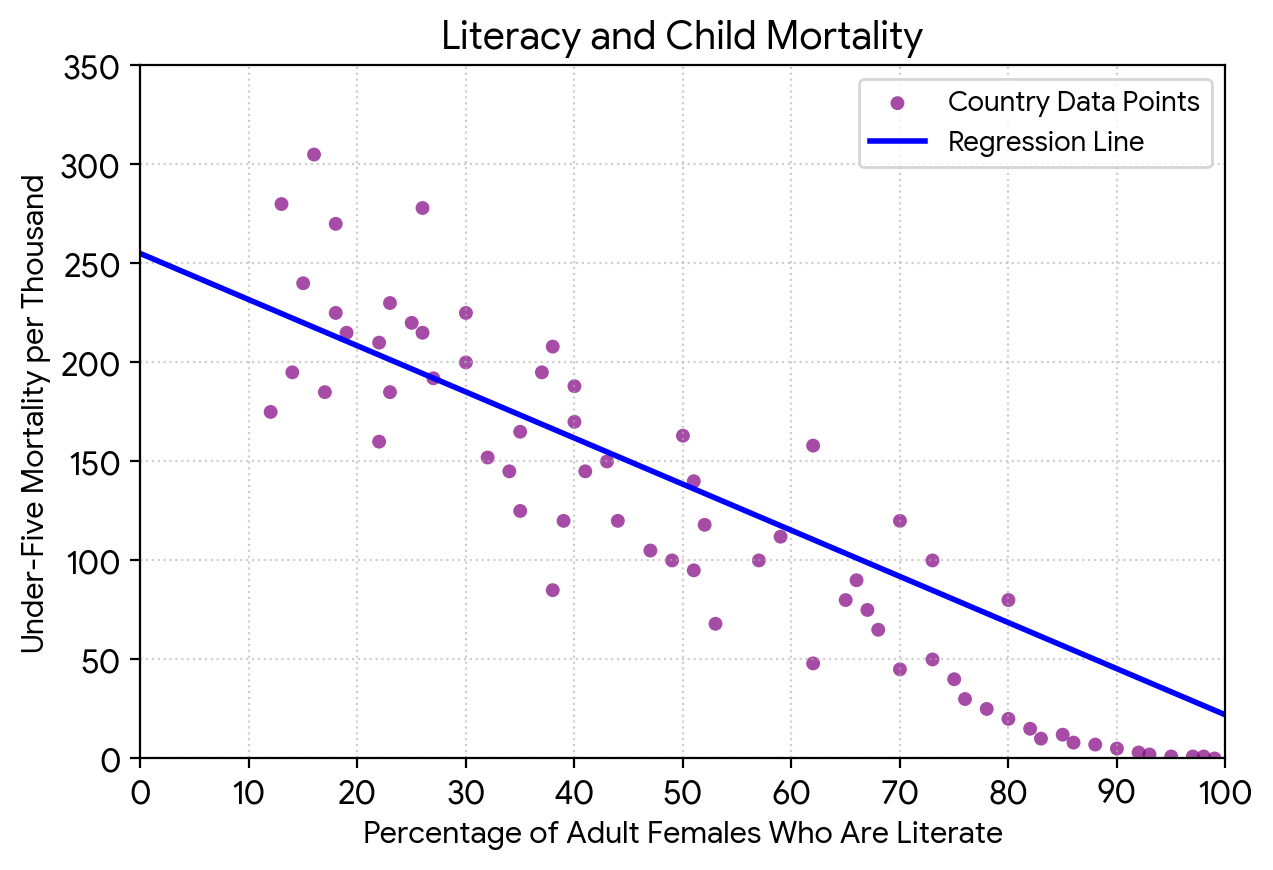
\includegraphics[width=\linewidth]{external/img-literacy-mortality.png}
\end{image}%
\tcblower
\end{figureptx}%
Use the provided chart to determine whether each of the following statements is \alert{True} or \alert{False}:%
\begin{enumerate}[label={\arabic*}]
\item{}There is a perfect negative correlation between the percentage of adult females who are literate and under-five mortality.%
\item{}As the percentage of adult females who are literate increases, under-five mortality tends to decrease.%
\item{}There is no correlation between the percentage of adult females who are literate and under-five mortality.%
\end{enumerate}
%
\par\smallskip%
\noindent\textbf{\blocktitlefont Solution}.\hypertarget{example-literacy-child-mortality-3}{}\quad{}By evaluating the direction and spatial dispersion of the data clusters on the graph, we find the following solutions:%
\par
%
\begin{itemize}[label=\ptxlistdisc]
\item{}\alert{Statement 1 is False.} A \terminology{perfect negative correlation} (\(r = -1.0\)) requires every observed country node to land exactly on the blue trajectory pathway line. Because data nodes are spread out in a loose cloud formation above and below the trendline, the pairing represents a strong, imperfect negative correlation.%
\item{}\alert{Statement 2 is True.} The simple linear regression model features a distinct downward slope tracking from left to right. This confirms that as female literacy coordinates increase along the horizontal axis, the corresponding under-five mortality index shows a consistent, predictable decline.%
\item{}\alert{Statement 3 is False.} A condition of \terminology{no correlation} (\(r = 0\)) generates a completely unstructured cloud of circular nodes accompanied by a flat, zero-slope horizontal regression bar. This graph shows a clear linear pattern, proving a strong statistical relationship between the two metrics.%
\end{itemize}
%
\end{example}
\begin{assemblage}{Assemblage}{Simple Linear Regression.}{assemblage-linear-regression}%
\alert{Simple linear regression} is a statistical method that models the relationship between a single independent variable and a continuous dependent variable by fitting a linear equation to observed data. It plots a straight line of best fit. The equation of the line is typically expressed as a linear function of the form%
\begin{equation*}
Y = mx + b\text{,}
\end{equation*}
where \(m\) represents the slope of the line and \(b\) represents the y-intercept.%
\end{assemblage}
\begin{example}{Example}{}{example-widget-package}%
A linear model calculated from the dataset below yields a slope of 0.25 and a y-intercept of 8.25. The table details the relationship between the number of widgets in a package and the total length of the package, measured in inches.%
\begin{tableptx}{Table}{\textbf{}}{table-widget-data}{}%
\centering%
{\tabularfont%
\begin{tabular}{ll}\hrulethin
\multicolumn{1}{c}{\terminology{Number of Widgets (\(x\))}}&\multicolumn{1}{c}{\terminology{Length of Package in. (\(y\))}}\tabularnewline\hrulethin
\multicolumn{1}{c}{3}&\multicolumn{1}{c}{9.00}\tabularnewline\hrulethin
\multicolumn{1}{c}{4}&\multicolumn{1}{c}{9.25}\tabularnewline\hrulethin
\multicolumn{1}{c}{5}&\multicolumn{1}{c}{9.50}\tabularnewline\hrulethin
\multicolumn{1}{c}{6}&\multicolumn{1}{c}{9.75}\tabularnewline\hrulethin
\end{tabular}
}%
\end{tableptx}%
%
\begin{enumerate}[label={\alph*)}]
\item{}Form the equation of the regression line and interpret the slope and y-intercept in the context of the problem.%
\item{}Using the regression line, predict the length of a package that contains 7 widgets.%
\end{enumerate}
%
\par\smallskip%
\noindent\textbf{\blocktitlefont Solution}.\hypertarget{example-widget-package-2}{}\quad{}%
\begin{enumerate}[label={\alph*}]
\item{}Using the slope (\(m = 0.25\)) and the \(y\)\textunderscore{}-intercept (\(b = 8.25\)), the simple linear regression equation is:%
\begin{equation*}
Y = 8.25 + 0.25X
\end{equation*}
%
\par
\alert{Interpretation of the Slope:} For each additional widget added to the package (\(\Delta X = 1\)), the total length of the package increases by exactly \alert{0.25 inches}.%
\par
\alert{Interpretation of the y-Intercept:} When there are zero widgets in the package (\(X = 0\)), the baseline length of the packaging material itself is \alert{8.25 inches}.%
\item{}To predict the total packaging length for a shipment containing \(7\) widgets, substitute \(X = 7\) into our linear regression model:%
\begin{align*}
Y \amp= 8.25 + 0.25(7)\\
Y \amp= 8.25 + 1.75\\
Y \amp= 10.00 \text{ inches}
\end{align*}
A package holding 7 widgets is predicted to be exactly \alert{10.00 inches} long.%
\end{enumerate}
%
\begin{figureptx}{Figure}{Linear Regression Trend for Widget Packaging}{fig-widget-regression}{}%
\begin{image}{0.2}{0.6}{0.2}{}%
\resizebox{\linewidth}{!}{%
\begin{tikzpicture}
  \begin{axis}[
    xlabel={Number of Widgets ($x$)},
    ylabel={Length of Package in. ($y$)},
    xmin=2, xmax=7,
    ymin=8, ymax=11,
    grid=both,
    grid style={dashed, gray!30}
  ]
    \addplot[only marks, blue, mark=*] coordinates {(3,9.00) (4,9.25) (5,9.50) (6,9.75)};
    \addplot[red, thick, domain=2:7] {0.25*x + 8.25};
  \end{axis}
\end{tikzpicture}%
}%
\end{image}%
\tcblower
\end{figureptx}%
\end{example}
\begin{example}{Example}{}{example-fat-calories-regression}%
A linear model calculated from a dataset yields a slope of 13.3 and a y-intercept of 142.6 when modeling the relationship between total fat grams (\(x\)) and total calories (\(y\)) in a selection of fast food sandwiches.%
\par
%
\begin{enumerate}[label={\alph*}]
\item{}Form the linear regression equation that models this data, rounding all baseline parameters to the nearest integer, and interpret the slope and y-intercept in the context of the problem.%
\item{}Using the regression model, predict the total number of calories in a menu item that contains 25 grams of fat. Round your final prediction to the nearest whole integer.%
\end{enumerate}
%
\begin{tableptx}{Table}{\textbf{}}{table-sandwich-nutrition}{}%
\centering%
{\tabularfont%
\begin{tabular}{cc}\hrulethin
{\bfseries{}\terminology{Total Fat g (\(x\))}}&{\bfseries{}\terminology{Total Calories (\(y\))}}\tabularnewline\hrulethin
9&260\tabularnewline\hrulethin
13&320\tabularnewline\hrulethin
21&420\tabularnewline\hrulethin
30&530\tabularnewline\hrulethin
31&560\tabularnewline\hrulethin
32&580\tabularnewline\hrulethin
34&590\tabularnewline\hrulethin
\end{tabular}
}%
\end{tableptx}%
\par\smallskip%
\noindent\textbf{\blocktitlefont Solution}.\hypertarget{example-fat-calories-regression-2}{}\quad{}%
\begin{enumerate}[label={\alph*}]
\item{}Rounding the y-intercept (\(142.6 \approx 143\)) and the slope (\(13.3 \approx 13\)), the linear regression equation is:%
\begin{equation*}
Y = 143 + 13X
\end{equation*}
%
\par
\alert{Slope Interpretation:} For each additional 1 gram of fat in a sandwich, the energy content is predicted to increase by approximately \alert{13 calories}.%
\par
\alert{y-Intercept Interpretation:} If a sandwich contains 0 grams of fat, its predicted baseline energy value from non-fat ingredients is \alert{143 calories}.%
\item{}Substitute \(X = 25\) into the unrounded regression line equation to find the precise calorie projection:%
\begin{align*}
Y \amp= 142.6 + 13.3(25)\\
Y \amp= 475.1 \approx 475 \text{ calories}
\end{align*}
An item with 25 grams of fat is estimated to contain \alert{475 calories}.%
\end{enumerate}
%
\begin{figureptx}{Figure}{Linear Fit of Fat Content to Total Calories}{fig-sandwich-regression}{}%
\begin{image}{0.2}{0.6}{0.2}{}%
\resizebox{\linewidth}{!}{%
\begin{tikzpicture}
  \begin{axis}[
    xlabel={Total Fat g ($x$)},
    ylabel={Total Calories ($y$)},
    xmin=0, xmax=40,
    ymin=200, ymax=700,
    grid=both,
    grid style={dashed, gray!30}
  ]
    \addplot[only marks, blue, mark=*] coordinates {
      (9,260) (13,320) (21,420) (30,530) (31,560) (32,580) (34,590)
    };
    \addplot[red, thick, domain=0:40] {13.305*x + 142.595};
  \end{axis}
\end{tikzpicture}%
}%
\end{image}%
\tcblower
\end{figureptx}%
\end{example}
\begin{inlineexercise}{Checkpoint}{}{exercise-eclipse-temperature}%
During a solar eclipse, the temperature begins to drop as the Moon comes between the Earth and the Sun. The cooling temperatures, up through totality, of the eclipse are shown in the table below. Using a linear regression equation with the slope -4.4 and y-intercept 75.1, predict the temperature at the 4 minute mark during the cooling, to the nearest degree.%
\begin{tableptx}{Table}{\textbf{}}{table-eclipse-data}{}%
\centering%
{\tabularfont%
\begin{tabular}{cc}\hrulethin
{\bfseries{}\terminology{Time minutes (\(x\))}}&{\bfseries{}\terminology{Temp. \(^\circ\)F (\(y\))}}\tabularnewline\hrulethin
0&75\tabularnewline\hrulethin
1&71\tabularnewline\hrulethin
2&66\tabularnewline\hrulethin
3&62\tabularnewline\hrulethin
4&?\tabularnewline\hrulethin
\end{tabular}
}%
\end{tableptx}%
Select the predicted temperature at the 4 minute mark.%
\par\smallskip%
\noindent\textbf{\blocktitlefont Solution}.\hypertarget{exercise-eclipse-temperature-2}{}\quad{}\terminology{Step 1: Calculate the Regression Equation} \(Y = -4.4x + 75.1\).%
\par
\terminology{Step 2: Evaluate at 4 Minutes} Substitute \(x = 4\) directly into our regression model to find the expected cooling value:%
\begin{align*}
Y \amp = -4.4(4) + 75.1\\
Y \amp = -17.6 + 75.1 = 57.5
\end{align*}
Rounding \(57.5^\circ\text{F}\) to the nearest whole integer gives our target choice of \terminology{58\(^\circ\)}.%
\begin{figureptx}{Figure}{Linear Regression Line for Eclipse Cooling Pattern}{fig-eclipse-regression}{}%
\begin{image}{0.2}{0.6}{0.2}{}%
\resizebox{\linewidth}{!}{%
\begin{tikzpicture}
  \begin{axis}[
    xlabel={Time in minutes ($x$)},
    ylabel={Temperature $^\circ$F ($y$)},
    xmin=-0.5, xmax=4.5,
    ymin=55, ymax=80,
    grid=both,
    grid style={dashed, gray!30}
  ]
    \addplot[only marks, blue, mark=*] coordinates {(0,75) (1,71) (2,66) (3,62)};
    \addplot[red, thick, domain=-0.5:4.5] {-4.4*x + 75.1};
    \addplot[only marks, green, mark=x, mark size=4pt, thick] coordinates {(4,57.5)};
  \end{axis}
\end{tikzpicture}%
}%
\end{image}%
\tcblower
\end{figureptx}%
\end{inlineexercise}%
\begin{inlineexercise}{Checkpoint}{}{exercise-coat-campaign}%
A morning radio talk show is running a \textquotedblleft{}Winter Coat Campaign\textquotedblright{} to collect and deliver coats to local shelters. They are storing the coats until they reach their goal of 2100 coats. The table below shows the number of coats in storage at the end of each day of the campaign.%
\begin{tableptx}{Table}{\textbf{}}{table-coat-data}{}%
\centering%
{\tabularfont%
\begin{tabular}{cc}\hrulethin
{\bfseries{}\terminology{Day of Campaign (\(x\))}}&{\bfseries{}\terminology{Number of Coats Stored (\(y\))}}\tabularnewline\hrulethin
1&860\tabularnewline\hrulethin
2&930\tabularnewline\hrulethin
3&1000\tabularnewline\hrulethin
4&1150\tabularnewline\hrulethin
5&1200\tabularnewline\hrulethin
6&1360\tabularnewline\hrulethin
\end{tabular}
}%
\end{tableptx}%
Find the linear regression equation with the slope 98.86 and y-intercept 737.33 rounded to the nearest hundredths, and predict the day the campaign will meet its goal.%
\par\smallskip%
\noindent\textbf{\blocktitlefont Solution}.\hypertarget{exercise-coat-campaign-2}{}\quad{}\terminology{Part a) Linear Regression Equation:} Thus, the linear modeling line of best fit is%
\begin{equation*}
Y = 98.86x + 737.33
\end{equation*}
%
\par
\terminology{Part b) Goal Prediction:} To compute the target milestone, substitute \(Y = 2100\) into the verified equation:%
\begin{align*}
2100 \amp = 98.86x + 737.33\\
1362.67 \amp = 98.86x\\
x \amp \approx 13.78
\end{align*}
Because the data tracks totals at the end of each day, reaching \(13.78\) means the campaign will successfully complete its goal on \terminology{Day 14}.%
\begin{figureptx}{Figure}{Linear Path Tracking Coat Collection Goal Delivery}{fig-coat-regression}{}%
\begin{image}{0.2}{0.6}{0.2}{}%
\resizebox{\linewidth}{!}{%
\begin{tikzpicture}
  \begin{axis} [
    xlabel={Day of Campaign ($x$)},
    ylabel={Number of Coats Stored ($y$)},
    xmin=0, xmax=15,
    ymin=600, ymax=2300,
    grid=both,
    grid style={dashed, gray!30}
  ]
    \addplot[only marks, blue, mark=*] coordinates {
      (1,860) (2,930) (3,1000) (4,1150) (5,1200) (6,1360)
    };
    \addplot[red, thick, domain=0:15] {98.857*x + 737.333};
    \addplot[gray, dashed, domain=0:15] {2100};
    \addplot[only marks, green, mark=x, mark size=4pt, thick] coordinates {(13.78,2100)};
  \end{axis}
\end{tikzpicture}%
}%
\end{image}%
\tcblower
\end{figureptx}%
\end{inlineexercise}%
\end{sectionptx}
%
%
\typeout{************************************************}
\typeout{Section  4.6 Chapter Exercises}
\typeout{************************************************}
%
\begin{sectionptx}{Section}{4.6 Chapter Exercises}{}{4.6 Chapter Exercises}{}{}{sec-stat-ch-ex}
%
%
\typeout{************************************************}
\typeout{Exercises  Statistics Practice Problem}
\typeout{************************************************}
%
\begin{exercises-subsection-numberless}{Exercises}{Statistics Practice Problem}{}{Statistics Practice Problem}{}{}{sec-stat-ch-ex-2}
\begin{divisionexercise}{1}{}{}{ex-mean-median-mode}%
Find the mean, median, and mode for the following dataset:%
\begin{equation*}
\{29, 24, 31, 40, 30, 35, 25, 28\}
\end{equation*}
%
\par\smallskip%
\noindent\textbf{\blocktitlefont Solution}.\hypertarget{ex-mean-median-mode-2}{}\quad{}To simplify the statistical calculations, we first arrange the dataset of \(n = 8\) values in ascending order:%
\begin{equation*}
\{24, 25, 28, 29, 30, 31, 35, 40\}
\end{equation*}
%
\par
\terminology{1. Mean Calculation:} The mean is calculated by summing all the values and dividing by the total number of data points (\(n = 8\)):%
\begin{align*}
\text{Mean} \amp = \frac{24 + 25 + 28 + 29 + 30 + 31 + 35 + 40}{8}\\
\text{Mean} \amp = \frac{242}{8} = 30.25
\end{align*}
Thus, the mean of the dataset is \terminology{30.25}.%
\par
\terminology{2. Median Calculation:} Since there is an even number of data points (\(8\)), the median is found by taking the average of the two middle values (the 4th and 5th numbers in our ordered list, which are \(29\) and \(30\)):%
\begin{equation*}
\text{Median} = \frac{29 + 30}{2} = 29.5
\end{equation*}
Thus, the median of the dataset is \terminology{29.5}.%
\par
\terminology{3. Mode Calculation:} The mode is the value that appears most frequently in a dataset. Because every unique number in this list occurs exactly once, there is \terminology{no mode}.%
\end{divisionexercise}%
\begin{divisionexercise}{2}{}{}{exercise-approx-sd-twenties}%
Use the data 20, 24, 34, 38. Without actually computing the standard deviation, which of the following best approximates the standard deviation?%
\par
%
\begin{enumerate}[label={\Alph*.}]
\item{}2%
\item{}4%
\item{}8%
\item{}10%
\end{enumerate}
%
\par\smallskip%
\noindent\textbf{\blocktitlefont Answer}.\hypertarget{exercise-approx-sd-twenties-2}{}\quad{}C.%
\par\smallskip%
\noindent\textbf{\blocktitlefont Solution}.\hypertarget{exercise-approx-sd-twenties-3}{}\quad{}%
\begin{enumerate}[label={\Alph*.}]
\item{}\lititle{Incorrect.}\par%
Incorrect. The data points span a total range of 18 units (from 20 to 38), so they sit much further than 2 units away from the center.%
\item{}\lititle{Incorrect.}\par%
Incorrect. While 4 is a factor, the data points are spread out further from the mean of 29 than this value suggests.%
\item{}\lititle{Correct.}\par%
Correct. The mean is 29. The data points sit 5 and 9 units away from this mean. An average distance of roughly 7-8 units is the most accurate estimate.%
\item{}\lititle{Incorrect.}\par%
Incorrect. This value overestimates the standard deviation, as most points are closer to the mean than 10 units.%
\end{enumerate}
%
\end{divisionexercise}%
\begin{divisionexercise}{3}{}{}{exercise-rainfall-approx-sd}%
The rainfall in a small town is recorded daily for two weeks, in inches:%
\begin{equation*}
\{1.2, 2.3, 0.8, 2.3, 1.0, 3.1, 4.2, 1.4, 2.1, 0.4, 1.3, 2.0, 1.8, 3.2\}
\end{equation*}
What are the mean and the approximate sample standard deviation for this data set?%
\par\smallskip%
\noindent\textbf{\blocktitlefont Solution}.\hypertarget{exercise-rainfall-approx-sd-2}{}\quad{}Step 1: Calculate the Mean. Sum all 14 data entries and divide by the count:%
\begin{equation*}
Mean = \frac{27.1}{14} \approx 1.94\text{ inches}
\end{equation*}
%
\par
Step 2: Find individual distances. Find the absolute difference between each entry and the mean of \(1.94\). Summing these 14 positive distances gives \(11.3\).%
\par
Step 3: Average the distances. Divide the sum of distances by the number of values:%
\begin{equation*}
\text{Average Distance} = \frac{11.3}{14} \approx 0.81
\end{equation*}
%
\par
Step 4: Approximate Standard Deviation. Because the geometric process of squaring numbers shifts standard deviation upwards, the true standard deviation value will sit slightly higher than our baseline average distance. We can approximate the sample standard deviation to be \terminology{just above 0.81} (approximately \(0.9\) to \(1.0\)).%
\end{divisionexercise}%
\begin{divisionexercise}{4}{}{}{ex-empirical-rule-heights}%
The heights of adult men in a certain city are normally distributed with a mean of 70 inches and a standard deviation (\(\text{SD}\)) of 3 inches. Use the Empirical Rule to answer the following questions:%
\begin{enumerate}[label={\alph*)}]
\item{}What percentage of men are between 67 and 73 inches tall?%
\item{}What percentage of men are between 61 and 79 inches tall?%
\item{}What percentage of men are taller than 76 inches?%
\end{enumerate}
%
\par\smallskip%
\noindent\textbf{\blocktitlefont Solution}.\hypertarget{ex-empirical-rule-heights-2}{}\quad{}The \terminology{Empirical Rule} (also known as the 68-95-99.7 rule) states that for a perfectly normal distribution:%
\begin{itemize}[label=\ptxlistdisc]
\item{}Approximately \(68\%\) of the data falls within \(1\) standard deviation of the mean (\(\pm 1\text{SD}\)).%
\item{}Approximately \(95\%\) of the data falls within \(2\) standard deviations of the mean (\(\pm 2\text{SD}\)).%
\item{}Approximately \(99.7\%\) of the data falls within \(3\) standard deviations of the mean (\(\pm 3\text{SD}\)).%
\end{itemize}
%
\par
Given parameters: \(Mean = 70\) inches and Standard Deviation \(\text{SD} = 3\) inches. Let us map out the standard deviation markers:%
\begin{itemize}[label=\ptxlistdisc]
\item{}mean\(\pm 1\text{SD} = 70 \pm 3 = [67, 73]\)%
\item{}mean\(\pm 2\text{SD} = 70 \pm 6 = [64, 76]\)%
\item{}mean\(\pm 3\text{SD} = 70 \pm 9 = [61, 79]\)%
\end{itemize}
%
\par
\terminology{Part a) Interval [67, 73]:} These values correspond exactly to mean\(- 1\text{SD}\) and mean\(+ 1\text{SD}\). According to the rule, approximately \terminology{68\%} of the men fall within this height range.%
\par
\terminology{Part b) Interval [61, 79]:} These values correspond exactly to mean \(- 3\text{SD}\) and mean \(+ 3\text{SD}\). According to the rule, approximately \terminology{99.7\%} of the men fall within this height range.%
\par
\terminology{Part c) Heights above 76 inches:} A height of 76 inches corresponds exactly to mean\(+ 2\text{SD}\). Since a normal curve is perfectly symmetrical, \(50\%\) of the data falls above the mean of 70. The region between the mean (70) and 2 standard deviations above the mean (76) contains exactly half of the \(95\%\) range, which is \(47.5\%\). To find the tail value remaining above 76:%
\begin{equation*}
50\% - 47.5\% = 2.5\%
\end{equation*}
Thus, approximately \terminology{2.5\%} of men in the city are taller than 76 inches.%
\begin{figureptx}{Figure}{Normal Distribution of Heights with Empirical Rule Breakdowns}{fig-empirical-bell-curve}{}%
\begin{image}{0.125}{0.75}{0.125}{}%
\resizebox{\linewidth}{!}{%
\begin{tikzpicture}
  [declare function={normalpdf(\x,\mu,\sigma)=1/(\sigma*sqrt(2*pi))*exp(-(\x-\mu)^2/(2*\sigma^2));}]
  \begin{axis}[
    xlabel={Height in Inches},
    ylabel={},
    xmin=58, xmax=82,
    ymin=0, ymax=0.15,
    axis y line=none,
    axis x line=bottom,
    xtick={61,64,67,70,73,76,79},
    height=5cm, width=11cm,
    enlargelimits=false
  ]
    \addplot [fill=blue!10, draw=none, domain=58:82] {normalpdf(x,70,3)} \closedcycle;
    \addplot [fill=blue!30, draw=none, domain=67:73] {normalpdf(x,70,3)} \closedcycle;
    \addplot [thick, blue, domain=58:82, samples=100] {normalpdf(x,70,3)};
    
    % Standard Deviation Reference Bounds
    \draw [dashed, gray] (axis cs:70,0) -- (axis cs:70,0.133);
    \draw [dashed, gray!80] (axis cs:67,0) -- (axis cs:67,0.08);
    \draw [dashed, gray!80] (axis cs:73,0) -- (axis cs:73,0.08);
    \draw [dashed, gray!60] (axis cs:64,0) -- (axis cs:64,0.015);
    \draw [dashed, gray!60] (axis cs:76,0) -- (axis cs:76,0.015);
    
    % Percentage Coverage Labels
    \node at (axis cs:70,0.04) {68\%};
    \draw [<->, thick, red] (axis cs:64,0.11) -- (axis cs:76,0.11) node[midway, fill=white] {95\%};
    \draw [<->, thick, black] (axis cs:61,0.13) -- (axis cs:79,0.13) node[midway, fill=white] {99.7\%};
  \end{axis}
\end{tikzpicture}%
}%
\end{image}%
\tcblower
\end{figureptx}%
\end{divisionexercise}%
\begin{divisionexercise}{5}{}{}{ex-ski-price}%
What is the z-score of the price of a pair of skis that cost \textdollar{}247, if the mean ski price is \textdollar{}279, with a standard deviation of \textdollar{}16?%
\par\smallskip%
\noindent\textbf{\blocktitlefont Solution}.\hypertarget{ex-ski-price-2}{}\quad{}Identify the given parameters: value \(x = 247\), mean \(= 279\), and standard deviation \(sd = 16\).%
\par
Substitute these values into the z-score formula:%
\begin{equation*}
z = \frac{247 - 279}{16} = \frac{-32}{16} = -2.0
\end{equation*}
%
\par
The price of the skis is exactly \terminology{2.0 standard deviations below} the mean.%
\begin{figureptx}{Figure}{Normal distribution curve highlighting a z-score of -2.0.}{fig-tikz-ski-zscore}{}%
\begin{image}{0.2}{0.6}{0.2}{}%
\resizebox{\linewidth}{!}{%
\begin{tikzpicture}[
  declare function={normalpdf(\x,\mu,\sigma)=1/(\sigma*sqrt(2*pi))*exp(-(\x-\mu)^2/(2*\sigma^2));}
]
  \begin{axis}[
    axis lines=left,
    xlabel={$z$},
    ylabel={},
    xmin=-4, xmax=4,
    ymin=0, ymax=0.45,
    ticks=none,
    enlargelimits=false,
    axis x line=bottom,
    axis y line=none,
    height=5cm, width=8cm
  ]
    \addplot [fill=blue!10, draw=none, domain=-4:4] {normalpdf(x,0,1)} \closedcycle;
    \addplot [thick, blue, domain=-4:4, samples=100] {normalpdf(x,0,1)};
    \draw [dashed, red, thick] (axis cs:-2, 0) -- (axis cs:-2, {normalpdf(-2,0,1)});
    \node[red, above] at (axis cs:-2, {normalpdf(-2,0,1)}) {$z = -2.0$};
    \draw [dashed, gray] (axis cs:0, 0) -- (axis cs:0, {normalpdf(0,0,1)});
    \node[gray, below] at (axis cs:0, 0) {$0$};
  \end{axis}
\end{tikzpicture}%
}%
\end{image}%
\tcblower
\end{figureptx}%
\end{divisionexercise}%
\begin{divisionexercise}{6}{}{}{ex-ice-cream-scoops}%
What is the z-score of a 5-scoop ice cream cone if the mean number of scoops is 3, with a standard deviation of 1 scoop?%
\par\smallskip%
\noindent\textbf{\blocktitlefont Solution}.\hypertarget{ex-ice-cream-scoops-2}{}\quad{}Identify the given parameters: value \(x = 5\), mean \(= 3\), and standard deviation \(sd = 1\).%
\par
Substitute these values into the z-score formula:%
\begin{equation*}
z = \frac{5 - 3}{1} = \frac{2}{1} = 2.0
\end{equation*}
%
\par
The 5-scoop cone is exactly \terminology{2.0 standard deviations above} the mean.%
\begin{figureptx}{Figure}{Normal distribution curve highlighting a z-score of 2.0.}{fig-tikz-icecream-zscore}{}%
\begin{image}{0.2}{0.6}{0.2}{}%
\resizebox{\linewidth}{!}{%
\begin{tikzpicture}[
  declare function={normalpdf(\x,\mu,\sigma)=1/(\sigma*sqrt(2*pi))*exp(-(\x-\mu)^2/(2*\sigma^2));}
]
  \begin{axis}[
    axis lines=left,
    xlabel={$z$},
    ylabel={},
    xmin=-4, xmax=4,
    ymin=0, ymax=0.45,
    ticks=none,
    enlargelimits=false,
    axis x line=bottom,
    axis y line=none,
    height=5cm, width=8cm
  ]
    \addplot [fill=blue!10, draw=none, domain=-4:4] {normalpdf(x,0,1)} \closedcycle;
    \addplot [thick, blue, domain=-4:4, samples=100] {normalpdf(x,0,1)};
    \draw [dashed, red, thick] (axis cs:2, 0) -- (axis cs:2, {normalpdf(2,0,1)});
    \node[red, above] at (axis cs:2, {normalpdf(2,0,1)}) {$z = 2.0$};
    \draw [dashed, gray] (axis cs:0, 0) -- (axis cs:0, {normalpdf(0,0,1)});
    \node[gray, below] at (axis cs:0, 0) {$0$};
  \end{axis}
\end{tikzpicture}%
}%
\end{image}%
\tcblower
\end{figureptx}%
\end{divisionexercise}%
\begin{divisionexercise}{7}{}{}{ex-cow-weight}%
What is the z-score of the weight of a cow that tips the scales at 825 lbs, if the mean weight for cows of her type is 1150 lbs, with a standard deviation of 77 lbs?%
\par\smallskip%
\noindent\textbf{\blocktitlefont Solution}.\hypertarget{ex-cow-weight-2}{}\quad{}Identify the given parameters: value \(x = 825\), mean \(= 1150\), and standard deviation \(sd = 77\).%
\par
Substitute these values into the z-score formula and round to two decimal places:%
\begin{equation*}
z = \frac{825 - 1150}{77} = \frac{-325}{77} \approx -4.22
\end{equation*}
%
\par
The cow's weight is approximately \terminology{4.22 standard deviations below} the mean.%
\begin{figureptx}{Figure}{Normal distribution curve highlighting an extreme z-score of -4.22.}{fig-tikz-cow-zscore}{}%
\begin{image}{0.2}{0.6}{0.2}{}%
\resizebox{\linewidth}{!}{%
\begin{tikzpicture}[
  declare function={normalpdf(\x,\mu,\sigma)=1/(\sigma*sqrt(2*pi))*exp(-(\x-\mu)^2/(2*\sigma^2));}
]
  \begin{axis}[
    axis lines=left,
    xlabel={$z$},
    ylabel={},
    xmin=-5, xmax=4,
    ymin=0, ymax=0.45,
    ticks=none,
    enlargelimits=false,
    axis x line=bottom,
    axis y line=none,
    height=5cm, width=8cm
  ]
    \addplot [fill=blue!10, draw=none, domain=-5:4] {normalpdf(x,0,1)} \closedcycle;
    \addplot [thick, blue, domain=-5:4, samples=100] {normalpdf(x,0,1)};
    \draw [dashed, red, thick] (axis cs:-4.22, 0) -- (axis cs:-4.22, 0.05);
    \node[red, above] at (axis cs:-4.22, 0.05) {$z \approx -4.22$};
    \draw [dashed, gray] (axis cs:0, 0) -- (axis cs:0, {normalpdf(0,0,1)});
    \node[gray, below] at (axis cs:0, 0) {$0$};
  \end{axis}
\end{tikzpicture}%
}%
\end{image}%
\tcblower
\end{figureptx}%
\end{divisionexercise}%
\begin{divisionexercise}{8}{}{}{ex-decimal-measurement}%
What is the z-score of a measured value of 0.0034, given mean \(= 0.0041\) and \(sd = 0.0008\)?%
\par\smallskip%
\noindent\textbf{\blocktitlefont Solution}.\hypertarget{ex-decimal-measurement-2}{}\quad{}Identify the given parameters: value \(x = 0.0034\), mean \(= 0.0041\), and standard deviation \(sd = 0.0008\).%
\par
Substitute these values into the standard z-score formula:%
\begin{equation*}
z = \frac{x - mean}{sd} = \frac{0.0034 - 0.0041}{0.0008} = \frac{-0.0007}{0.0008} = -0.875
\end{equation*}
%
\par
The measured value is exactly \terminology{0.875 standard deviations below} the population mean.%
\begin{figureptx}{Figure}{Normal distribution curve highlighting a z-score of -0.875.}{fig-tikz-decimal-zscore}{}%
\begin{image}{0.2}{0.6}{0.2}{}%
\resizebox{\linewidth}{!}{%
\begin{tikzpicture}[
  declare function={normalpdf(\x,\mu,\sigma)=1/(\sigma*sqrt(2*pi))*exp(-(\x-\mu)^2/(2*\sigma^2));}
]
  \begin{axis}[
    axis lines=left,
    xlabel={$z$},
    ylabel={},
    xmin=-4, xmax=4,
    ymin=0, ymax=0.45,
    ticks=none,
    enlargelimits=false,
    axis x line=bottom,
    axis y line=none,
    height=5cm, width=8cm
  ]
    \addplot [fill=blue!10, draw=none, domain=-4:4] {normalpdf(x,0,1)} \closedcycle;
    \addplot [thick, blue, domain=-4:4, samples=100] {normalpdf(x,0,1)};
    \draw [dashed, red, thick] (axis cs:-0.875, 0) -- (axis cs:-0.875, {normalpdf(-0.875,0,1)});
    \node[red, above] at (axis cs:-0.875, {normalpdf(-0.875,0,1)}) {$z = -0.875$};
    \draw [dashed, gray] (axis cs:0, 0) -- (axis cs:0, {normalpdf(0,0,1)});
    \node[gray, below] at (axis cs:0, 0) {$0$};
  \end{axis}
\end{tikzpicture}%
}%
\end{image}%
\tcblower
\end{figureptx}%
\end{divisionexercise}%
\begin{divisionexercise}{9}{}{}{ex-student-test-score}%
What is the z-score of a student's test score of 89, if the class average was 80 with a standard deviation of 4 points?%
\par\smallskip%
\noindent\textbf{\blocktitlefont Solution}.\hypertarget{ex-student-test-score-2}{}\quad{}Identify the given parameters: raw score \(x = 89\), class mean \(= 80\), and standard deviation \(sd = 4\).%
\par
Substitute these values into the z-score expression:%
\begin{equation*}
z = \frac{x - mean}{sd} = \frac{89 - 80}{4} = \frac{9}{4} = 2.25
\end{equation*}
%
\par
The student's test performance translates to a z-score of \terminology{2.25}, meaning it is \terminology{2.25 standard deviations above} the classroom average.%
\begin{figureptx}{Figure}{Normal distribution curve highlighting a z-score of 2.25.}{fig-tikz-test-zscore}{}%
\begin{image}{0.2}{0.6}{0.2}{}%
\resizebox{\linewidth}{!}{%
\begin{tikzpicture}[
  declare function={normalpdf(\x,\mu,\sigma)=1/(\sigma*sqrt(2*pi))*exp(-(\x-\mu)^2/(2*\sigma^2));}
]
  \begin{axis}[
    axis lines=left,
    xlabel={$z$},
    ylabel={},
    xmin=-4, xmax=4,
    ymin=0, ymax=0.45,
    ticks=none,
    enlargelimits=false,
    axis x line=bottom,
    axis y line=none,
    height=5cm, width=8cm
  ]
    \addplot [fill=blue!10, draw=none, domain=-4:4] {normalpdf(x,0,1)} \closedcycle;
    \addplot [thick, blue, domain=-4:4, samples=100] {normalpdf(x,0,1)};
    \draw [dashed, red, thick] (axis cs:2.25, 0) -- (axis cs:2.25, {normalpdf(2.25,0,1)});
    \node[red, above] at (axis cs:2.25, {normalpdf(2.25,0,1)}) {$z = 2.25$};
    \draw [dashed, gray] (axis cs:0, 0) -- (axis cs:0, {normalpdf(0,0,1)});
    \node[gray, below] at (axis cs:0, 0) {$0$};
  \end{axis}
\end{tikzpicture}%
}%
\end{image}%
\tcblower
\end{figureptx}%
\end{divisionexercise}%
\begin{divisionexercise}{10}{}{}{exercise-kori-monthly-budget}%
Kori categorized her spending for this month into four categories: food, rent, fun, and other. The percentage she spent in each category is displayed in the chart below.%
\begin{figureptx}{Figure}{Pie Chart of Kori's Monthly Spending Shares}{fig-kori-budget-pie-chart}{}%
\begin{image}{0.175}{0.65}{0.175}{}%
\resizebox{\linewidth}{!}{%
\begin{tikzpicture}[scale=1.3]
  % Rent slice: 0 to 111.6 degrees (31%)
  \draw[fill=blue!20, draw=black] (0,0) -- (0:2) arc (0:111.6:2) -- cycle;
  \node at (55.8:1.4) {\small 31\%};
  \node at (55.8:2.4) {\small Rent};

  % Other slice: 111.6 to 216.0 degrees (111.6 + 104.4 = 29%)
  \draw[fill=gray!20, draw=black] (0,0) -- (111.6:2) arc (111.6:216.0:2) -- cycle;
  \node at (163.8:1.4) {\small 29\%};
  \node at (163.8:2.4) {\small Other};

  % Food slice: 216.0 to 302.4 degrees (216.0 + 86.4 = 24%)
  \draw[fill=green!20, draw=black] (0,0) -- (216.0:2) arc (216.0:302.4:2) -- cycle;
  \node at (259.2:1.4) {\small 24\%};
  \node at (259.2:2.4) {\small Food};

  % Fun slice: 302.4 to 360.0 degrees (302.4 + 57.6 = 16%)
  \draw[fill=orange!20, draw=black] (0,0) -- (302.4:2) arc (302.4:360.0:2) -- cycle;
  \node at (331.2:1.4) {\small 16\%};
  \node at (331.2:2.4) {\small Fun};
\end{tikzpicture}%
}%
\end{image}%
\tcblower
\end{figureptx}%
If she spent a total of \(\$2600\) this month, how much money did she allocate to rent?%
\par\smallskip%
\noindent\textbf{\blocktitlefont Solution}.\hypertarget{exercise-kori-monthly-budget-2}{}\quad{}To find the exact dollar amount spent on rent, we convert the percentage share from the pie chart into a decimal and multiply it by the total monthly expenditures:%
\par
%
\begin{equation*}
\text{Rent Share} = 31\% = 0.31
\end{equation*}
%
\par
%
\begin{equation*}
\text{Rent Expenditures} = 0.31 \times \$2600 = \$806
\end{equation*}
%
\par
Therefore, Kori spent exactly \alert{\(\$806\)} on rent this month.%
\end{divisionexercise}%
\begin{divisionexercise}{11}{}{}{exer-women-height-distribution}%
Suppose the height of adult women in the United States is normally distributed with a mean of 5' 8" and a standard deviation of \(1.5\)". What is the probability that a randomly chosen woman in the United States is shorter than 5' 5"?%
\begin{figureptx}{Figure}{Normal distribution curve of women's heights with the lower tail below 5' 5" shaded.}{fig-women-height-tail}{}%
\begin{image}{0.1}{0.8}{0.1}{}%
\resizebox{\linewidth}{!}{%
\begin{tikzpicture}[x=1.2cm, y=10cm]

% Shaded lower tail region (below -2 standard deviations)
\fill[blue!30] plot[domain=-3.5:-2, samples=20] (\x, {1/(sqrt(2*3.14159))*exp(-\x*\x/2)}) -- (-2,0) -- (-3.5,0) -- cycle;

% Draw the normal distribution curve
\draw[very thick, black] plot[domain=-3.5:3.5, samples=50] (\x, {1/(sqrt(2*3.14159))*exp(-\x*\x/2)});

% Vertical dashed standard deviation lines
\draw[gray!40, dashed] (-3, 0) -- (-3, 0.0044);
\draw[gray!40, dashed] (-2, 0) -- (-2, 0.054);
\draw[gray!40, dashed] (-1, 0) -- (-1, 0.242);
\draw[gray!40, dashed] (0, 0)  -- (0, 0.398);
\draw[gray!40, dashed] (1, 0)  -- (1, 0.242);
\draw[gray!40, dashed] (2, 0)  -- (2, 0.054);
\draw[gray!40, dashed] (3, 0)  -- (3, 0.0044);

% Simple flat horizontal base axis line
\draw[thick] (-3.5, 0) -- (3.5, 0);

% Height Labels on Axis
\node[below=2pt] at (0, 0)  {5'8''};
\node[below=2pt] at (1, 0)  {5'9.5''};
\node[below=2pt] at (-1, 0) {5'6.5''};
\node[below=2pt] at (2, 0)  {5'11''};
\node[below=2pt] at (-2, 0) {5'5''};
\node[below=2pt] at (3, 0)  {6'0.5''};
\node[below=2pt] at (-3, 0) {5'3.5''};

% Label pointing out the shaded 2.5% area
\node[text=blue!80!black, font=\small] at (-2.6, 0.06) {2.5\%};
\draw[thick, blue!80!black] (-2.5, 0.04) -- (-2.2, 0.01);

\end{tikzpicture}%
}%
\end{image}%
\tcblower
\end{figureptx}%
\par\smallskip%
\noindent\textbf{\blocktitlefont Solution}.\hypertarget{exer-women-height-distribution-2}{}\quad{}First, determine how many standard deviations 5' 5" is from the mean of 5'8". Since each standard deviation is \(1.5\)", a height of 5' 6.5" is \(1\) standard deviation below the mean, and 5' 5" is exactly \(2\) standard deviations below the mean.%
\par
We can find the total percentage of women who are 5' 5" or taller by adding up the known regions of the normal distribution:%
%
\begin{itemize}[label=\ptxlistdisc]
\item{}50\% of women are taller than the mean of 5' 8".%
\item{}34\% of women are between 5' 6.5" and 5' 8" (within \(1\) standard deviation below the mean).%
\item{}13.5\% of women are between 5' 5" and 5' 6.5" (between \(1\) and \(2\) standard deviations below the mean).%
\end{itemize}
Adding these regions together gives: \(50\% + 34\% + 13.5\% = 97.5\%\). Since 97.5\% of women are 5' 5" or taller, the remaining portion is \(100\% - 97.5\% = 2.5\%\).%
\par
\emph{Alternative Method:} The empirical rule states that 95\% of the data falls within \(2\) standard deviations of the mean. This leaves 5\% split equally between the two extreme outer tails (\(5\% \div 2 = 2.5\%\)). Therefore, the probability that a randomly chosen woman is shorter than 5' 5" is 2.5\% (or \(0.025\)).%
\end{divisionexercise}%
\begin{divisionexercise}{12}{Positive Correlation: Summer Heatwaves and Ice Cream Sales.}{}{exercise-ice-cream-prediction}%
A beachside shop owner wants to examine the relationship between the daily afternoon temperature (\(X\), measured in degrees Fahrenheit) and the number of ice cream cones sold daily (\(Y\)). The data collected over a five-day period is presented below.%
\begin{tableptx}{Table}{\textbf{Daily Temperature vs. Ice Cream Sales}}{table-ice-cream-data}{}%
\centering%
{\tabularfont%
\begin{tabular}{AcAcAcA}\hrulethin
{\bfseries{}Day}&{\bfseries{}Temperature (\(X\) in \(^\circ\text{F}\))}&{\bfseries{}Ice Cream Cones Sold (\(Y\))}\tabularnewline\hrulemedium
1&70&100\tabularnewline\hrulethin
2&75&150\tabularnewline\hrulethin
3&80&190\tabularnewline\hrulethin
4&85&260\tabularnewline\hrulethin
5&90&300\tabularnewline\hrulethin
\end{tabular}
}%
\end{tableptx}%
Using the simple linear regression model calculated from the observed data table above, predict the total number of ice cream cones sold if the afternoon temperature reaches \(100^\circ\text{F}\).%
\par
%
\begin{enumerate}[label={\Alph*.}]
\item{}340 cones%
\item{}404 cones%
\item{}450 cones%
\item{}512 cones%
\end{enumerate}
%
\par\smallskip%
\noindent\textbf{\blocktitlefont Answer}.\hypertarget{exercise-ice-cream-prediction-3}{}\quad{}B.%
\par\smallskip%
\noindent\textbf{\blocktitlefont Solution 1}.\hypertarget{exercise-ice-cream-prediction-4}{}\quad{}To predict the number of ice cream cones sold at 100°F, we first need to graph the data points from the table and calculate the line of best fit using linear regression.%
\par
 \begin{figureptx}{Figure}{Scatter Plot of Temperature vs. Ice Cream Cones Sold}{figure-ice-cream-scatter}{}%
\begin{image}{0}{1}{0}{}%
\resizebox{\linewidth}{!}{%
\begin{tikzpicture}
    \begin{axis}[
        xlabel={Temperature ($^\circ$F)},
        ylabel={Cones Sold},
        xmin=65, xmax=105,
        ymin=50, ymax=450,
        xtick={70,75,80,85,90,95,100},
        ytick={100,150,200,250,300,350,400},
        grid=both,
        grid style={line width=.1pt, color=gray!10},
        major grid style={line width=.2pt, color=gray!50},
        legend pos=north west
    ]
    
    
    \addplot[
        domain=65:105,
        color=red,
        thick,
        samples=2
    ] {-616 + 10.2*x};
    \addlegendentry{Regression Line}

    
    \addplot[
        only marks,
        mark=*,
        color=blue,
        mark size=3pt,
        nodes near coords,
        point meta=explicit symbolic,
        every node near coord/.style={anchor=south east, font=\footnotesize, color=black}
    ] coordinates {
        (70,100) [Day 1]
        (75,150) [Day 2]
        (80,190) [Day 3]
        (85,260) [Day 4]
        (90,300) [Day 5]
    };
    \addlegendentry{Observed Data Points}

    \end{axis}
\end{tikzpicture}%
}%
\end{image}%
\tcblower
\end{figureptx}%
%
\par\smallskip%
\noindent\textbf{\blocktitlefont Solution 2}.\hypertarget{exercise-ice-cream-prediction-5}{}\quad{}%
\begin{enumerate}[label={\Alph*.}]
\item{}\lititle{Incorrect.}\par%
Incorrect. This value underestimates the strong upward trend observed as the temperature steps up to 100 degrees.%
\item{}\lititle{Correct.}\par%
Correct! Observe the data points and plug directly into the line: \(404\).%
\item{}\lititle{Incorrect.}\par%
Incorrect. While sales are rising fast, this estimate is slightly higher than what the mathematical trend line predicts.%
\item{}\lititle{Incorrect.}\par%
Incorrect. This value assumes exponential growth rather than a steady simple linear progression rate.%
\end{enumerate}
%
\end{divisionexercise}%
\begin{divisionexercise}{13}{}{}{ex-product-popularity}%
A store is doing inventory for one week to determine the popularity of a new product. The table below shows the number of items sold each day. Find the linear regression equation that models this data with the slope 8.66 and y-intercept 14.57, rounding coefficients to the nearest integer. Then, predict the number of items sold on the 10th day if the pattern of growth continues.%
\begin{tableptx}{Table}{\textbf{}}{table-sales-data}{}%
\centering%
{\tabularfont%
\begin{tabular}{cc}\hrulethin
{\bfseries{}\terminology{Day Number (\(x\))}}&{\bfseries{}\terminology{Number Sold (\(y\))}}\tabularnewline\hrulethin
1&24\tabularnewline\hrulethin
2&32\tabularnewline\hrulethin
3&41\tabularnewline\hrulethin
4&50\tabularnewline\hrulethin
5&60\tabularnewline\hrulethin
6&68\tabularnewline\hrulethin
7&77\tabularnewline\hrulethin
\end{tabular}
}%
\end{tableptx}%
\par\smallskip%
\noindent\textbf{\blocktitlefont Solution}.\hypertarget{ex-product-popularity-2}{}\quad{}\terminology{Step 1: Calculate the Regression Equation} The linear regression equation is given by \(y = mx + b\), where \(m\) is the slope and \(b\) is the y-intercept. Substituting the provided values, we have:%
\begin{equation*}
Y = 8.66x + 14.57
\end{equation*}
Rounding the coefficients to the nearest integer gives us the simplified regression equation:%
\begin{equation*}
Y = 9x + 15
\end{equation*}
%
\par
\terminology{Step 2: Predict for Day 10} To estimate item performance on the tenth day, we evaluate our regression equation at \(x = 10\):%
\begin{align*}
Y \amp = 9(10) + 15\\
Y \amp = 90 + 15 = 105
\end{align*}
Rounding to the nearest whole item integer yields a final estimate of \terminology{105} items sold.%
\begin{figureptx}{Figure}{Linear Regression Mapping Weekly Product Growth}{fig-sales-regression}{}%
\begin{image}{0.2}{0.6}{0.2}{}%
\resizebox{\linewidth}{!}{%
\begin{tikzpicture}
  \begin{axis}[
    xlabel={Day Number ($x$)},
    ylabel={Number Sold ($y$)},
    xmin=0, xmax=12,
    ymin=0, ymax=120,
    grid=both,
    grid style={dashed, gray!30}
  ]
    \addplot[only marks, blue, mark=*] coordinates {
      (1,24) (2,32) (3,41) (4,50) (5,60) (6,68) (7,77)
    };
    \addplot[red, thick, domain=0:12] {8.857*x + 14.571};
    \addplot[only marks, green, mark=x, mark size=4pt, thick] coordinates {(10,103.14)};
  \end{axis}
\end{tikzpicture}%
}%
\end{image}%
\tcblower
\end{figureptx}%
\end{divisionexercise}%
\end{exercises-subsection-numberless}
\end{sectionptx}
\end{chapterptx}
%
%
\typeout{************************************************}
\typeout{Chapter 5 MyOpenMath Interactive Activities}
\typeout{************************************************}
%
\begin{chapterptx}{Chapter}{MyOpenMath Interactive Activities}{}{MyOpenMath Interactive Activities}{}{}{activities}
\renewcommand*{\chaptername}{Chapter}
\begin{introduction}{}%
These files contain copies of the interactive MyOpenMath exercises that guided our learning for each topic. Special thanks to Professor Jason Hardin for sharing his MyOpenMath question bank.%
\end{introduction}%
%
%
\typeout{************************************************}
\typeout{Worksheet  01. Activity Voting Methods}
\typeout{************************************************}
%
\newgeometry{left=0.75in, right=0.75in, top=0.75in, bottom=0.75in}
\begin{worksheet-section}{Worksheet}{01. Activity Voting Methods}{}{01. Activity Voting Methods}{}{}{activity-01-intro-activity}
\begin{introduction}{}%
In many decision making situations, it is necessary to gather the group consensus using some sort of vote. While the basic idea of voting is fairly universal, the method by which those votes are used to determine a winner can vary. In deciding upon a winner, there is always one main goal: to reflect the preferences of the people in the most fair way possible. We will discuss four different methods for determining the winner of an election using preference ballots, and will see that we can sometimes have different winners under different methods of voting.%
\end{introduction}%
See \hyperref[notes-Voting]{Section~} for the voting notes.%
\begin{divisionexercise}{1}{}{2in}{activity-01-intro-activity-4-1}%
Four candidates are running for president of the Worcester State Math Club:  Alan (A), Brenda (B), Craig (C), and Diane (D). The club members are asked to submit preference ballots and the results are shown in the preference table below.%
\begin{center}%
{\tabularfont%
\begin{tabular}{llllll}
 & \(\displaystyle{19}\) &\(\displaystyle{15}\) &\(\displaystyle{11}\) &\(\displaystyle{7}\) &\(\displaystyle{2}\) \tabularnewline[0pt]
First&\(\displaystyle{B}\) &\(\displaystyle{C}\) &\(\displaystyle{D}\) &\(\displaystyle{A}\) &\(\displaystyle{C}\) \tabularnewline[0pt]
Second&\(\displaystyle{A}\) &\(\displaystyle{A}\) &\(\displaystyle{C}\) &\(\displaystyle{D}\) &\(\displaystyle{D}\) \tabularnewline[0pt]
Third&\(\displaystyle{C}\) &\(\displaystyle{D}\) &\(\displaystyle{A}\) &\(\displaystyle{C}\) &\(\displaystyle{A}\) \tabularnewline[0pt]
Fourth&\(\displaystyle{D}\) &\(\displaystyle{B}\) &\(\displaystyle{B}\) &\(\displaystyle{B}\) &\(\displaystyle{B}\) 
\end{tabular}
}%
\end{center}%
Note: All parts of the questions must be correct to earn credit!%
\par
How many students are in the Math Club?%
\par
\fillintext{20}%
\par
How many members have Craig as their first choice?%
\par
\fillintext{20}%
\par
How many members have Brenda as their last choice?%
\par
\fillintext{20}%
\par\smallskip%
\noindent\textbf{\blocktitlefont Answer}.\hypertarget{activity-01-intro-activity-4-1-2}{}\quad{}%
\begin{itemize}[label=\ptxlistdisc]
\item{}54%
\item{}17%
\item{}35%
\end{itemize}
%
\end{divisionexercise}%
\clearpage
\begin{divisionexercise}{2}{}{2in}{activity-01-intro-activity-5-1}%
Which of the following voting methods will we discuss in this course. Select all that apply!%
\par
%
\begin{enumerate}[label={(\alph*)}]
\item{}Plurality method%
\item{}Hamilton's method%
\item{}Plurality with elimination method%
\item{}Pairwise comparison method%
\item{}Jefferson's method%
\item{}Borda count method%
\end{enumerate}
%
\par\smallskip%
\noindent\textbf{\blocktitlefont Answer}.\hypertarget{activity-01-intro-activity-5-1-2}{}\quad{}%
\begin{itemize}[label=\ptxlistdisc]
\item{}Plurality method%
\par
Plurality with elimination method%
\par
Borda count method%
\par
Pairwise comparison method%
\end{itemize}
%
\end{divisionexercise}%
\clearpage
\begin{divisionexercise}{3}{}{2in}{activity-01-intro-activity-6-1}%
Four candidates are running for president of the Worcester State Math Club: Alan (A), Brenda (B), Craig (C), and Diane (D). The club members are asked to submit preference ballots and the results are shown in the preference table below.%
\begin{center}%
{\tabularfont%
\begin{tabular}{llllll}
 & \(\displaystyle{19}\) &\(\displaystyle{15}\) &\(\displaystyle{11}\) &\(\displaystyle{7}\) &\(\displaystyle{2}\) \tabularnewline[0pt]
First&\(\displaystyle{B}\) &\(\displaystyle{C}\) &\(\displaystyle{D}\) &\(\displaystyle{A}\) &\(\displaystyle{C}\) \tabularnewline[0pt]
Second&\(\displaystyle{A}\) &\(\displaystyle{A}\) &\(\displaystyle{C}\) &\(\displaystyle{D}\) &\(\displaystyle{D}\) \tabularnewline[0pt]
Third&\(\displaystyle{C}\) &\(\displaystyle{D}\) &\(\displaystyle{A}\) &\(\displaystyle{C}\) &\(\displaystyle{A}\) \tabularnewline[0pt]
Fourth&\(\displaystyle{D}\) &\(\displaystyle{B}\) &\(\displaystyle{B}\) &\(\displaystyle{B}\) &\(\displaystyle{B}\) 
\end{tabular}
}%
\end{center}%
Note: All parts of the questions must be correct to earn credit!%
\par
Who would win the election under the plurality method?%
\par
%
\begin{enumerate}[label={(\alph*)}]
\item{}Alan%
\item{}Brenda%
\item{}Craig%
\item{}Diane%
\end{enumerate}
%
\par
How many first place votes did this candidate receive?%
\par
\fillintext{20}%
\par
Does the winning candidate receive the majority of first place votes?%
\par
%
\begin{enumerate}[label={(\alph*)}]
\item{}Yes%
\item{}No%
\end{enumerate}
%
\par\smallskip%
\noindent\textbf{\blocktitlefont Answer}.\hypertarget{activity-01-intro-activity-6-1-2}{}\quad{}%
\begin{itemize}[label=\ptxlistdisc]
\item{}B: Brenda%
\item{}19%
\item{}B: No%
\end{itemize}
%
\end{divisionexercise}%
\clearpage
\begin{divisionexercise}{4}{}{2in}{activity-01-intro-activity-7-1}%
Four candidates are running for president of the Worcester State Math Club: Alan (A), Brenda (B), Craig (C), and Diane (D). The club members are asked to submit preference ballots and the results are shown in the preference table below.%
\begin{center}%
{\tabularfont%
\begin{tabular}{llllll}
 & \(\displaystyle{19}\) &\(\displaystyle{15}\) &\(\displaystyle{11}\) &\(\displaystyle{7}\) &\(\displaystyle{2}\) \tabularnewline[0pt]
First&\(\displaystyle{B}\) &\(\displaystyle{C}\) &\(\displaystyle{D}\) &\(\displaystyle{A}\) &\(\displaystyle{C}\) \tabularnewline[0pt]
Second&\(\displaystyle{A}\) &\(\displaystyle{A}\) &\(\displaystyle{C}\) &\(\displaystyle{D}\) &\(\displaystyle{D}\) \tabularnewline[0pt]
Third&\(\displaystyle{C}\) &\(\displaystyle{D}\) &\(\displaystyle{A}\) &\(\displaystyle{C}\) &\(\displaystyle{A}\) \tabularnewline[0pt]
Fourth&\(\displaystyle{D}\) &\(\displaystyle{B}\) &\(\displaystyle{B}\) &\(\displaystyle{B}\) &\(\displaystyle{B}\) 
\end{tabular}
}%
\end{center}%
Note: All parts of the questions must be correct to earn credit!%
\par
Who would be the first candidate eliminated under the plurality with elimination method?%
\par
%
\begin{enumerate}[label={(\alph*)}]
\item{}Alan%
\item{}Brenda%
\item{}Craig%
\item{}Diane%
\end{enumerate}
%
\par
After this candidate is eliminated and the votes are redistributed, how many first-choice votes does Diane have? (If Diane was the first eliminated, enter 0 as your answer here.)%
\par
\fillintext{20}%
\par
Who wins this election under plurality with elimination?%
\par
%
\begin{enumerate}[label={(\alph*)}]
\item{}Alan%
\item{}Brenda%
\item{}Craig%
\item{}Diane%
\end{enumerate}
%
\par\smallskip%
\noindent\textbf{\blocktitlefont Answer}.\hypertarget{activity-01-intro-activity-7-1-2}{}\quad{}%
\begin{itemize}[label=\ptxlistdisc]
\item{}A: Alan%
\item{}18%
\item{}D: Diane%
\end{itemize}
%
\end{divisionexercise}%
\clearpage
\begin{divisionexercise}{5}{}{2in}{activity-01-intro-activity-8-1}%
Four candidates are running for president of the Worcester State Math Club: Alan (A), Brenda (B), Craig (C), and Diane (D). The club members are asked to submit preference ballots and the results are shown in the preference table below.%
\begin{center}%
{\tabularfont%
\begin{tabular}{llllll}
 & \(\displaystyle{19}\) &\(\displaystyle{15}\) &\(\displaystyle{11}\) &\(\displaystyle{7}\) &\(\displaystyle{2}\) \tabularnewline[0pt]
First&\(\displaystyle{B}\) &\(\displaystyle{C}\) &\(\displaystyle{D}\) &\(\displaystyle{A}\) &\(\displaystyle{C}\) \tabularnewline[0pt]
Second&\(\displaystyle{A}\) &\(\displaystyle{A}\) &\(\displaystyle{C}\) &\(\displaystyle{D}\) &\(\displaystyle{D}\) \tabularnewline[0pt]
Third&\(\displaystyle{C}\) &\(\displaystyle{D}\) &\(\displaystyle{A}\) &\(\displaystyle{C}\) &\(\displaystyle{A}\) \tabularnewline[0pt]
Fourth&\(\displaystyle{D}\) &\(\displaystyle{B}\) &\(\displaystyle{B}\) &\(\displaystyle{B}\) &\(\displaystyle{B}\) 
\end{tabular}
}%
\end{center}%
Note: All parts of the questions must be correct to earn credit!%
\par
Who would win the election under the Borda count method?%
\par
%
\begin{enumerate}[label={(\alph*)}]
\item{}Alan%
\item{}Brenda%
\item{}Craig%
\item{}Diane%
\end{enumerate}
%
\par
How many points would the winning candidate receive under the Borda count?%
\par
\fillintext{20}%
\par\smallskip%
\noindent\textbf{\blocktitlefont Answer}.\hypertarget{activity-01-intro-activity-8-1-2}{}\quad{}%
\begin{itemize}[label=\ptxlistdisc]
\item{}A: Alan%
\item{}156%
\end{itemize}
%
\end{divisionexercise}%
\clearpage
\begin{divisionexercise}{6}{}{2in}{activity-01-intro-activity-9-1}%
Four candidates are running for president of the Worcester State Math Club: Alan (A), Brenda (B), Craig (C), and Diane (D). The club members are asked to submit preference ballots and the results are shown in the preference table below.%
\begin{center}%
{\tabularfont%
\begin{tabular}{llllll}
 & \(\displaystyle{19}\) &\(\displaystyle{15}\) &\(\displaystyle{11}\) &\(\displaystyle{7}\) &\(\displaystyle{2}\) \tabularnewline[0pt]
First&\(\displaystyle{B}\) &\(\displaystyle{C}\) &\(\displaystyle{D}\) &\(\displaystyle{A}\) &\(\displaystyle{C}\) \tabularnewline[0pt]
Second&\(\displaystyle{A}\) &\(\displaystyle{A}\) &\(\displaystyle{C}\) &\(\displaystyle{D}\) &\(\displaystyle{D}\) \tabularnewline[0pt]
Third&\(\displaystyle{C}\) &\(\displaystyle{D}\) &\(\displaystyle{A}\) &\(\displaystyle{C}\) &\(\displaystyle{A}\) \tabularnewline[0pt]
Fourth&\(\displaystyle{D}\) &\(\displaystyle{B}\) &\(\displaystyle{B}\) &\(\displaystyle{B}\) &\(\displaystyle{B}\) 
\end{tabular}
}%
\end{center}%
Note: All parts of the questions must be correct to earn credit!%
\par
Who would win the election under the pairwise comparison method?%
\par
%
\begin{enumerate}[label={(\alph*)}]
\item{}Alan%
\item{}Brenda%
\item{}Craig%
\item{}Diane%
\end{enumerate}
%
\par
How many points would the winning candidate receive under the pairwise comparison method?%
\par
\fillintext{20}%
\par\smallskip%
\noindent\textbf{\blocktitlefont Answer}.\hypertarget{activity-01-intro-activity-9-1-2}{}\quad{}%
\begin{itemize}[label=\ptxlistdisc]
\item{}C: Craig%
\item{}3%
\end{itemize}
%
\end{divisionexercise}%
\clearpage
\begin{divisionexercise}{7}{}{2in}{activity-01-intro-activity-10-1}%
We have seen four different methods for determining the winner of an election. Through our examples and problems, we have also seen that these different methods can lead to different winners! In particular, in the Math Club President election considered throughout the exercises, it turns out that each of the four voting methods leads to each of the four candidates being declared the winner!%
\end{divisionexercise}%
\end{worksheet-section}
\restoregeometry
%
%
\typeout{************************************************}
\typeout{Worksheet  02. Activity Apportionment Methods}
\typeout{************************************************}
%
\newgeometry{left=0.75in, right=0.75in, top=0.75in, bottom=0.75in}
\begin{worksheet-section}{Worksheet}{02. Activity Apportionment Methods}{}{02. Activity Apportionment Methods}{}{}{activity-02-intro-activity}
Apportionment is the problem of dividing up a fixed number of things among groups of different sizes. In politics, this takes the form of allocating a limited number of representatives amongst voters. This problem, presumably, is older than the United States, but the best-known ways to solve it have their origins in the problem of assigning each state an appropriate number of representatives in the new Congress when the country was formed. Apportionment theory is also used in many non-political situations, such as staffing a hospital with the appropriate number of nurses per shift and allocating buses to cover a set of bus routes based on the number of passengers.%
 \par
The goal with any apportionment problem is to find a way to fairly distribute the items (e.g., doctors, buses, instructors) amoung the groups (e.g., clinics, routes, courses).%
 \par
We face several real-world restrictions in this distribution process:%
 %
\begin{enumerate}[label={\arabic*}]
\item{}The things being divided up can exist only in whole numbers.%
\item{}We must use all of the things being divided up, and we cannot use any more.%
\item{}Each group must get at least one of the things being divided up.%
\item{}The number of things assigned to each group should be at least approximately proportional to the population of the group. (Exact proportionality isn't possible because of the whole number requirement, but we should try to be close, and in any case, if Group A is larger than Group B, then Group B shouldn't get more of the things than Group A does.)%
\end{enumerate}
 In terms of the apportionment of the United States House of Representatives, these rules imply:%
 \par
%
\begin{enumerate}[label={\arabic*}]
\item{}We can only have whole representatives. Massachusetts can't have 8.4 representatives.%
\item{}We can only use the (currently) 435 representatives available. If one state gets another representative, another state has to lose one.%
\item{}Every state gets at least one representative.%
\item{}The number of representatives each state gets should be approximately proportional to the state population. This way, the number of constituents each representative has should be approximately equal.%
\end{enumerate}
%
 \par
There are many different methods for solving an apportionment problem. In this course, we will discuss three of them: Hamilton's method, Jefferson's method, and Adams method. The first step for each method will be to compute the standard divisor and standard quotas.%
See \hyperref[section-apportionment]{Section~} for the apportionment notes.%
\clearpage
\begin{divisionexercise}{1}{}{0.2in}{activity-02-intro-activity-3-1}%
Which of the following scenarios illustrates an apportionment problem? Select ALL that apply!%
\par
%
\begin{enumerate}[label={(\alph*)}]
\item{}The WSU Math Club needs to elect a president and will do so by selecting the candidate with the most votes.%
\item{}A school system purchases 500 new computers and must distribute them among 8 elementary schools based on the number of students at each school.%
\item{}A daycare must distribute 100 toys among 5 rooms based on the number of children in each room.%
\item{}Four people pool their money to buy 60 shares of a stock, and the shares are distributed among the four based on the amount each person contributes.%
\end{enumerate}
%
\par\smallskip%
\noindent\textbf{\blocktitlefont Answer}.\hypertarget{activity-02-intro-activity-3-1-2}{}\quad{}%
\begin{itemize}[label=\ptxlistdisc]
\item{}A daycare must distribute 100 toys among 5 rooms based on the number of children in each room.%
\par
Four people pool their money to buy 60 shares of a stock, and the shares are distributed among the four based on the amount each person contributes.%
\par
A school system purchases 500 new computers and must distribute them among 8 elementary schools based on the number of students at each school.%
\end{itemize}
%
\end{divisionexercise}%
\clearpage
\begin{divisionexercise}{2}{}{0.2in}{activity-02-intro-activity-4-1}%
Which of the following apportionment methods will we discuss in this course. Select all that apply!%
\par
%
\begin{enumerate}[label={(\alph*)}]
\item{}Hamilton's method%
\item{}Jefferson's method%
\item{}Adam's Method%
\item{}Borda count method%
\item{}Plurality method%
\item{}Plurality with elimination method%
\item{}Pairwise comparison method%
\end{enumerate}
%
\par\smallskip%
\noindent\textbf{\blocktitlefont Answer}.\hypertarget{activity-02-intro-activity-4-1-2}{}\quad{}%
\begin{itemize}[label=\ptxlistdisc]
\item{}Hamilton's method%
\par
Jefferson's method%
\par
Adam's Method%
\end{itemize}
%
\end{divisionexercise}%
\clearpage
\begin{divisionexercise}{3}{}{2in}{activity-02-intro-activity-5-1}%
An HMO has \(\displaystyle{40}\) doctors to be apportioned among four clinics (\(\displaystyle{A}\), \(\displaystyle{B}\) ,\(\displaystyle{C}\) , \(\displaystyle{D}\)). The HMO decides to apportion the doctors based on the average weekly patient load for each clinic, shown in the table below. Find the standard divisor and the standard quota for each clinic. Round all answers, including the standard divisor, to two decimal places!%
\begin{image}{0}{1}{0}{}%
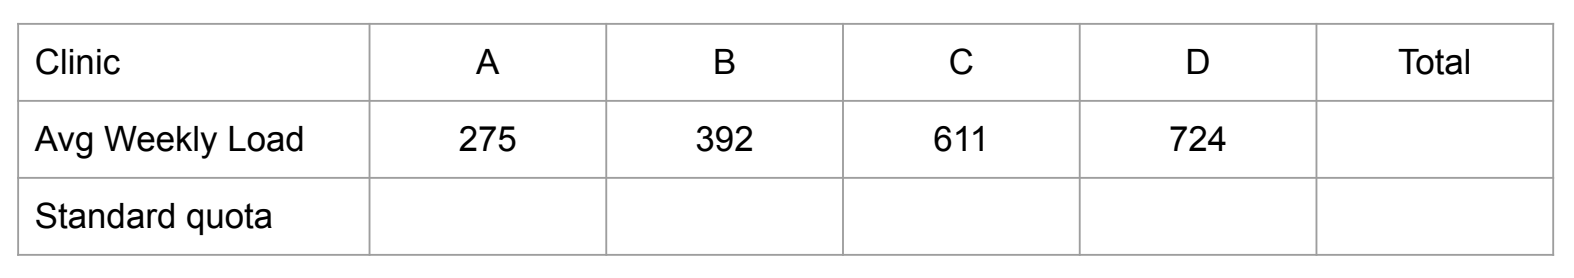
\includegraphics[width=\linewidth]{generated/problems/images/mom-1445060-1.PNG}
\end{image}%
Standard divisor = \fillintext{20}  %
\par
Standard quota for Clinic \(\displaystyle{A}\) = \fillintext{20}  %
\par
Standard quota for Clinic \(\displaystyle{B}\) = \fillintext{20}  %
\par
Standard quota for Clinic \(\displaystyle{C}\) = \fillintext{20}  %
\par
Standard quota for Clinic \(\displaystyle{D}\) = \fillintext{20}  %
\par\smallskip%
\noindent\textbf{\blocktitlefont Answer}.\hypertarget{activity-02-intro-activity-5-1-2}{}\quad{}%
\begin{itemize}[label=\ptxlistdisc]
\item{}50.05%
\item{}5.49%
\item{}7.83%
\item{}12.21%
\item{}14.47%
\end{itemize}
%
\end{divisionexercise}%
\clearpage
\begin{divisionexercise}{4}{}{2in}{activity-02-intro-activity-6-1}%
An HMO has \(\displaystyle{40}\) doctors to be apportioned among four clinics (\(\displaystyle{A}\), \(\displaystyle{B}\), \(\displaystyle{C}\), \(\displaystyle{D}\)). The HMO decides to apportion the doctors based on the average weekly patient load for each clinic, shown in the table below. Use Hamilton's method to apportion the doctors to the clinics.%
\par
Recall the standard divisor for this problem is \(\displaystyle{50.05}\).%
\begin{image}{0}{1}{0}{}%
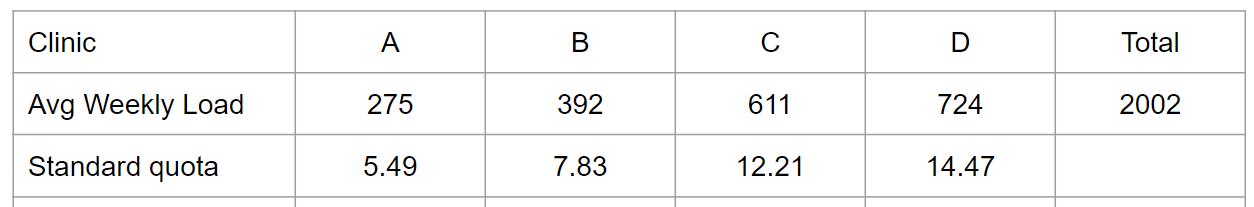
\includegraphics[width=\linewidth]{generated/problems/images/mom-1445078-1.PNG}
\end{image}%
Total doctors for Clinic \(\displaystyle{A}\) = \fillintext{20}  %
\par
Total doctors for Clinic \(\displaystyle{B}\) = \fillintext{20}  %
\par
Total doctors for Clinic \(\displaystyle{C}\) = \fillintext{20}  %
\par
Total doctors for Clinic \(\displaystyle{D}\) = \fillintext{20}  %
\par\smallskip%
\noindent\textbf{\blocktitlefont Answer}.\hypertarget{activity-02-intro-activity-6-1-2}{}\quad{}%
\begin{itemize}[label=\ptxlistdisc]
\item{}6%
\item{}8%
\item{}12%
\item{}14%
\end{itemize}
%
\end{divisionexercise}%
\clearpage
\begin{divisionexercise}{5}{}{2in}{activity-02-intro-activity-7-1}%
An HMO has \(\displaystyle{40}\) doctors to be apportioned among four clinics (\(\displaystyle{A}\), \(\displaystyle{B}\), \(\displaystyle{C}\), \(\displaystyle{D}\)). The HMO decides to apportion the doctors based on the average weekly patient load for each clinic, shown in the table below. Use Jefferson's method to apportion the doctors to the clinics.%
\par
Recall the standard divisor for this problem is \(\displaystyle{50.05}\).%
\begin{image}{0}{1}{0}{}%
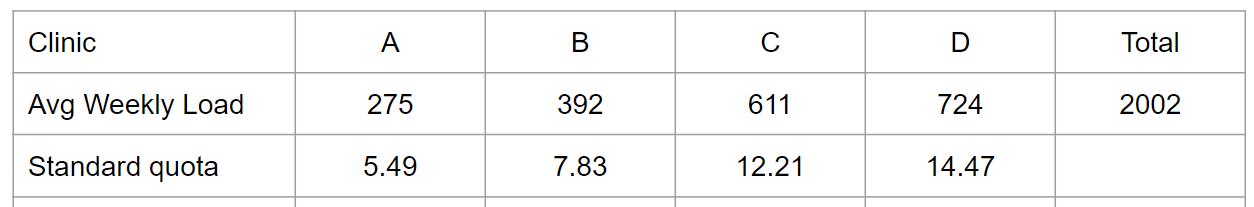
\includegraphics[width=\linewidth]{generated/problems/images/mom-1445079-1.PNG}
\end{image}%
Total doctors for Clinic \(\displaystyle{A}\) = \fillintext{20}  %
\par
Total doctors for Clinic \(\displaystyle{B}\) = \fillintext{20}  %
\par
Total doctors for Clinic \(\displaystyle{C}\) = \fillintext{20}  %
\par
Total doctors for Clinic \(\displaystyle{D}\) = \fillintext{20}  %
\par\smallskip%
\noindent\textbf{\blocktitlefont Answer}.\hypertarget{activity-02-intro-activity-7-1-2}{}\quad{}%
\begin{itemize}[label=\ptxlistdisc]
\item{}5%
\item{}8%
\item{}12%
\item{}15%
\end{itemize}
%
\end{divisionexercise}%
\clearpage
\begin{divisionexercise}{6}{}{2in}{activity-02-intro-activity-8-1}%
An HMO has \(\displaystyle{40}\) doctors to be apportioned among four clinics (\(\displaystyle{A}\), \(\displaystyle{B}\), \(\displaystyle{C}\), \(\displaystyle{D}\)). The HMO decides to apportion the doctors based on the average weekly patient load for each clinic, shown in the table below. Use Adams's method to apportion the doctors to the clinics.%
\par
Recall the standard divisor for this problem is \(\displaystyle{50.05}\).%
\begin{image}{0}{1}{0}{}%
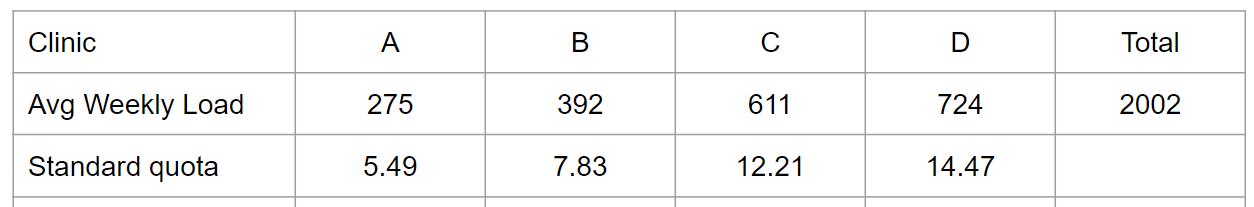
\includegraphics[width=\linewidth]{generated/problems/images/mom-1445082-1.PNG}
\end{image}%
Total doctors for Clinic \(\displaystyle{A}\) = \fillintext{20}  %
\par
Total doctors for Clinic \(\displaystyle{B}\) = \fillintext{20}  %
\par
Total doctors for Clinic \(\displaystyle{C}\) = \fillintext{20}  %
\par
Total doctors for Clinic \(\displaystyle{D}\) = \fillintext{20}  %
\par\smallskip%
\noindent\textbf{\blocktitlefont Answer}.\hypertarget{activity-02-intro-activity-8-1-2}{}\quad{}%
\begin{itemize}[label=\ptxlistdisc]
\item{}6%
\item{}8%
\item{}12%
\item{}14%
\end{itemize}
%
\end{divisionexercise}%
\end{worksheet-section}
\restoregeometry
%
%
\typeout{************************************************}
\typeout{Worksheet  03. Activity Simple Interest}
\typeout{************************************************}
%
\newgeometry{left=0.75in, right=0.75in, top=0.75in, bottom=0.75in}
\begin{worksheet-section}{Worksheet}{03. Activity Simple Interest}{}{03. Activity Simple Interest}{}{}{activity-03-intro-activity}
We have to work with money every day. While balancing your checkbook or calculating your monthly expenditures on coffee requires only arithmetic, when we start saving, planning for retirement, or need a loan, we need more mathematics!%
 \par
See \hyperref[notes-simple-interest]{Section~} for the simple interest notes.%
Discussing interest starts with the principal, which is the amount your account starts with. This could be a starting investment or the starting amount of a loan. Interest is the amount earned for depositing money or the amount paid for borrowing money. It is calculated as a percentage of the principal (called the interest rate) and is written as a decimal (for example, \(5\%\) is \(0.05\)).%
\par
For a simple example, if you borrowed \(\$100\) from a friend and agreed to repay it with \(5\%\) interest, then the amount of interest you would pay would just be \(5\%\) of \(\$100\):%
\begin{equation*}
\$100 \times 0.05 = \$5\text{.}
\end{equation*}
The total amount you would repay would be \(\$105\), which is the original principal plus the interest. This is an example of one-time simple interest, where the interest is calculated based on the principal only.%
\begin{divisionexercise}{1}{}{0.2in}{activity-03-intro-activity-2-4}%
Alex borrows \(\displaystyle\${1200}\) from their parents for college expenses and agrees to repay them with \(\displaystyle{7}\%\) interest.%
\par
a)  What is the principle in this situation?%
\par
\textdollar{} \fillintext{20}%
\par
b)  Write the interest rate as a decimal.%
\par
\fillintext{20} \%%
\par
c)  How much interest will Alex pay their parents?%
\par
\textdollar{} \fillintext{20}%
\par
d)  What is the total amount, principle plus interest, Alex will repay?%
\par
\textdollar{} \fillintext{20}%
\par\smallskip%
\noindent\textbf{\blocktitlefont Answer}.\hypertarget{activity-03-intro-activity-2-4-2}{}\quad{}%
\begin{itemize}[label=\ptxlistdisc]
\item{}1200%
\item{}0.07%
\item{}84%
\item{}1284%
\end{itemize}
%
\end{divisionexercise}%
\clearpage
One-time simple interest is only common for extremely short-term loans. For longer-term loans, it is common for interest to be paid on a daily, monthly, quarterly, or annual basis. In that case, interest would be earned regularly. For example, bonds are essentially a loan made to the bond issuer (a company or government) by you, the bondholder. In return for the loan, the issuer agrees to pay interest, often annually. Bonds have a maturity date, at which time the issuer pays back the original bond value.%
\begin{example}{Example}{}{activity-03-intro-activity-3-2}%
Suppose your city is building a new park, and issues bonds to raise the money to build it. You obtain a \(\$1,000\) bond that pays \(5\%\) interest annually that matures in \(5\) years. How much interest will you earn?%
\par\smallskip%
\noindent\textbf{\blocktitlefont Solution}.\hypertarget{activity-03-intro-activity-3-2-2}{}\quad{}Each year you would earn interest:%
\begin{equation*}
\$1,000 \times 0.05 = \$50\text{.}
\end{equation*}
So, over the course of five years, you would earn a total of%
\begin{equation*}
\$50 \times 5 = \$250\text{.}
\end{equation*}
When the bond matures, you would receive back the \(\$1,000\) you originally paid, leaving you with a total of \(\$1,250\).%
\end{example}
Notice how the amount of interest (\(I\)) was computed in this example: we multiplied the principal by the interest rate (represented as a decimal), then multiplied this by the number of years. We can generalize this idea of simple interest over time to obtain a formula that we can use to find the amount of simple interest earned:%
\begin{equation*}
I = Prt
\end{equation*}
where:%
\begin{itemize}[label=\ptxlistdisc]
\item{}\(I\) is the amount of simple interest%
\item{}\(P\) is the principal (starting amount)%
\item{}\(r\) is the interest rate represented as a decimal%
\item{}\(t\) is the time in years%
\end{itemize}
%
\begin{note}{Note}{}{activity-03-intro-activity-3-4}%
You do NOT need to memorize this formula! It will be provided for you on all quizzes and exams!%
\end{note}
Let's look at a quick example demonstrating the simple interest formula.%
\begin{example}{Example}{}{activity-03-intro-activity-3-6}%
A student took out a simple interest loan for \(\$5,000\) for \(3\) years at a rate of \(4\%\) to purchase a used car. What is the interest on the loan?%
\par\smallskip%
\noindent\textbf{\blocktitlefont Solution}.\hypertarget{activity-03-intro-activity-3-6-2}{}\quad{}We are given the following: \(P = \$5,000\), \(t = 3\), and \(r = 0.04\). Using the simple interest formula, the amount of interest on the loan is:%
\begin{equation*}
I = \$5,000 \times 0.04 \times 3 = \$600
\end{equation*}
%
\end{example}
\clearpage
\begin{divisionexercise}{2}{}{}{activity-03-intro-activity-4-1}%
In the simple interest formula \(\displaystyle{I}={P}{r}{t}\), what unit must \(\displaystyle{t}\) be given in?%
\par
%
\begin{enumerate}[label={(\alph*)}]
\item{}Weeks%
\item{}Months%
\item{}Days%
\item{}Quarters%
\item{}Years%
\item{}Decimals%
\item{}Whatever unit is given in the problem%
\item{}There is no particular unit%
\end{enumerate}
%
\par\smallskip%
\noindent\textbf{\blocktitlefont Answer}.\hypertarget{activity-03-intro-activity-4-1-2}{}\quad{}%
\begin{itemize}[label=\ptxlistdisc]
\item{}E: Years%
\end{itemize}
%
\end{divisionexercise}%
\begin{divisionexercise}{3}{}{}{activity-03-intro-activity-4-2}%
You take out a simple interest loan for \(\displaystyle\${500}\) for 3 years at an interest rate of \(\displaystyle{4}\%\)to pay for textbooks. What is the simple interest on the loan?%
\par
\textdollar{} \fillintext{20}%
\par\smallskip%
\noindent\textbf{\blocktitlefont Answer}.\hypertarget{activity-03-intro-activity-4-2-2}{}\quad{}%
\begin{itemize}[label=\ptxlistdisc]
\item{}60%
\end{itemize}
%
\end{divisionexercise}%
\clearpage
While finding the amount of interest accrued for a loan is important, it is perhaps more important that we determine the total amount that must be repaid. We will call this amount — that is, the total amount required to be repaid in a loan or the total amount earned in an investment — the \terminology{future value}. We will denote this quantity with the variable \(A\).%
\par
As we saw with the example on the previous page involving a city issuing bonds to build a new park, the future value of a loan can be found by adding together the principal and the interest. This is true for an investment as well. This will allow us to develop a formula for the future value involving simple interest:%
\begin{equation*}
A = P + I
\end{equation*}
Since \(I = Prt\), we can substitute this into the equation to get:%
\begin{equation*}
A = P + Prt = P(1 + rt)
\end{equation*}
This short calculation provides us with a formula for computing the future value for a simple interest loan or investment:%
\begin{equation*}
A = P(1 + rt)
\end{equation*}
where:%
\begin{itemize}[label=\ptxlistdisc]
\item{}\(A\) is the future value of the loan or investment%
\item{}\(P\) is the principal (starting amount) of the loan or investment%
\item{}\(r\) is the interest rate represented as a decimal%
\item{}\(t\) is the time in years%
\end{itemize}
%
\begin{note}{Note}{}{activity-03-intro-activity-5-3}%
You do NOT need to memorize this formula! It will be provided for you on all quizzes and exams!%
\end{note}
Let's look at a quick example demonstrating the simple interest formula.%
\begin{example}{Example}{}{activity-03-intro-activity-5-5}%
A loan of \(\$2,500\) has been made at \(6\%\) for \(9\) months. Find the loan’s future value.%
\par\smallskip%
\noindent\textbf{\blocktitlefont Solution}.\hypertarget{activity-03-intro-activity-5-5-2}{}\quad{}We are given the following: \(P = \$2,500\) and \(r = 0.06\).%
\par
For \(t\), note that we are given a time in months, not years! For the simple interest formula to be used correctly, we must give this value in years. Since there are \(12\) months in a year, we can always convert from months to years by dividing the number of months by \(12\). In this case, we have:%
\begin{equation*}
t = \frac{9}{12} = 0.75 \text{ years}
\end{equation*}
%
\par
Now, using the formula above we find a future value of:%
\begin{equation*}
A = \$2,500(1 + 0.06 \times 0.75) = \$2,612.50
\end{equation*}
%
\end{example}
\clearpage
\begin{divisionexercise}{4}{}{}{activity-03-intro-activity-6-1}%
Match each of the quantities on the left with the variable which represents it in the simple interest formula.%
\par
Note all answers must be correct to earn credit!%
\par
%
\begin{enumerate}[label={(\alph*)}]
\item{} Principle%
\item{} Interest rate%
\item{} Time%
\item{} Future value%
\end{enumerate}
%
\par
%
\begin{enumerate}[label={(\alph*)}]
\item{}\(\displaystyle \displaystyle{A}\)%
\item{}\(\displaystyle \displaystyle{t}\)%
\item{}\(\displaystyle \displaystyle{P}\)%
\item{}\(\displaystyle \displaystyle{r}\)%
\end{enumerate}
%
\par\smallskip%
\noindent\textbf{\blocktitlefont Answer}.\hypertarget{activity-03-intro-activity-6-1-2}{}\quad{}%
\begin{itemize}[label=\ptxlistdisc]
\item{}c d b a%
\end{itemize}
%
\end{divisionexercise}%
\begin{divisionexercise}{5}{}{}{activity-03-intro-activity-6-2}%
A simple interest loan is taken out for \(\displaystyle{6}\) months. What value of \(\displaystyle{t}\) should be used in the simple interest formula?%
\par
\(\displaystyle{t}=\) \fillintext{20}  %
\par\smallskip%
\noindent\textbf{\blocktitlefont Answer}.\hypertarget{activity-03-intro-activity-6-2-2}{}\quad{}%
\begin{itemize}[label=\ptxlistdisc]
\item{}0.5%
\end{itemize}
%
\end{divisionexercise}%
\begin{divisionexercise}{6}{}{}{activity-03-intro-activity-6-3}%
You deposit \(\displaystyle\${4500}\) in an investment paying a simple interest rate of \(\displaystyle{8}\%\). How much will the investment be worth in nine months?%
\par
\textdollar{} \fillintext{20}%
\par\smallskip%
\noindent\textbf{\blocktitlefont Answer}.\hypertarget{activity-03-intro-activity-6-3-2}{}\quad{}%
\begin{itemize}[label=\ptxlistdisc]
\item{}4770%
\end{itemize}
%
\end{divisionexercise}%
\clearpage
In addition to determining the future value for a simple interest loan or investment, the simple interest formula can be used to solve other types of problems. We might want to know how much we should deposit into an account with a given simple interest rate to ensure we have a given amount in the future. Or, like in the example below, we might want to determine the simple interest rate based on the principal and future values.%
\begin{example}{Example}{}{activity-03-intro-activity-7-2}%
You borrow \(\$500\) from a friend and promise to pay back \(\$560\) in \(18\) months. What simple interest rate will you pay?%
\par\smallskip%
\noindent\textbf{\blocktitlefont Solution}.\hypertarget{activity-03-intro-activity-7-2-2}{}\quad{}We are given the following: \(P = \$500\), \(A = \$560\), and \(t = \frac{18}{12} = 1.5\) years.%
\par
We are looking to find the value of \(r\) (hence, the "?"). We substitute the given values into the simple interest formula and solve for \(r\):%
\begin{equation*}
A = P(1 + rt)
\end{equation*}
%
\begin{equation*}
560 = 500(1 + r \times 1.5)
\end{equation*}
%
\par
Divide both sides by \(500\):%
\begin{equation*}
1.12 = 1 + 1.5r
\end{equation*}
Subtract \(1\) from both sides:%
\begin{equation*}
0.12 = 1.5r
\end{equation*}
Divide by \(1.5\):%
\begin{equation*}
r = \frac{0.12}{1.5} = 0.08
\end{equation*}
%
\par
Since \(r = 0.08\), we convert this to a percent to get a simple interest rate of \(8\%\).%
\end{example}
\begin{divisionexercise}{7}{}{2in}{activity-03-intro-activity-7-3}%
What was the primary goal in the preceding example?%
\par
%
\begin{enumerate}[label={(\alph*)}]
\item{}To find the future value of a loan.%
\item{}To find the amount deposited in a loan.%
\item{}To find the amount of time for which a loan was given.%
\item{}To find the simple interest rate for a loan.%
\item{}To find the amount of interest accrued over the course of a loan.%
\item{}None of the above.%
\end{enumerate}
%
\par\smallskip%
\noindent\textbf{\blocktitlefont Answer}.\hypertarget{activity-03-intro-activity-7-3-2}{}\quad{}%
\begin{itemize}[label=\ptxlistdisc]
\item{}D: To find the simple interest rate for a loan.%
\end{itemize}
%
\end{divisionexercise}%
\end{worksheet-section}
\restoregeometry
%
%
\typeout{************************************************}
\typeout{Worksheet  04. Activity Compound Interest}
\typeout{************************************************}
%
\newgeometry{left=0.75in, right=0.75in, top=0.75in, bottom=0.75in}
\begin{worksheet-section}{Worksheet}{04. Activity Compound Interest}{}{04. Activity Compound Interest}{}{}{activity-04-intro-activity}
With simple interest, we were assuming that we pocketed the interest when we received it. In a standard bank account, any interest we earn is automatically added to our balance, and we earn interest on that interest in future years. This reinvestment of interest is called \alert{compounding}.%
 \par
See \hyperref[notes-compound-interest]{Section~} for the compound interest notes.%
Suppose that we deposit \(\$1,000\) in a bank account offering \(12\%\) simple interest. After \(1\) year, the account would have a balance of \(\$1,120\).%
\par
Now, suppose that we deposit our \(\$1,000\) in a bank account offering \(12\%\) interest, compounded monthly. How will our money grow?%
\par
In the first month (note we use \(t = \frac{1}{12}\) so that time is given in years!):%
\begin{equation*}
I = \$1,000 \times 0.12 \times \frac{1}{12} = \$10
\end{equation*}
In the first month, we will earn \(\$10\) in interest, raising our account balance to \(\$1,010\).%
\par
In the second month:%
\begin{equation*}
I = \$1,010 \times 0.12 \times \frac{1}{12} = \$10.10
\end{equation*}
Notice that in the second month we earned more interest than we did in the first month. This is because we earned interest not only on the original \(\$1,000\) we deposited, but we also earned interest on the \(\$10\) of interest we earned the first month. This is the key advantage that compounding of interest gives us.%
\par
Calculating out a few more months, we obtain the following:%
\begin{center}%
{\tabularfont%
\begin{tabular}{AcAcAcAcA}\hrulethin
{\bfseries{}Month}&{\bfseries{}Starting Balance}&{\bfseries{}Interest Earned}&{\bfseries{}Ending Balance}\tabularnewline\hrulethin
1&\textdollar{}1,000.00&\textdollar{}10.00&\textdollar{}1,010.00\tabularnewline\hrulethin
2&\textdollar{}1,010.00&\textdollar{}10.10&\textdollar{}1,020.10\tabularnewline\hrulethin
3&\textdollar{}1,020.10&\textdollar{}10.20&\textdollar{}1,030.30\tabularnewline\hrulethin
4&\textdollar{}1,030.30&\textdollar{}10.30&\textdollar{}1,040.60\tabularnewline\hrulethin
5&\textdollar{}1,040.60&\textdollar{}10.41&\textdollar{}1,051.01\tabularnewline\hrulethin
6&\textdollar{}1,051.01&\textdollar{}10.51&\textdollar{}1,061.52\tabularnewline\hrulethin
7&\textdollar{}1,061.52&\textdollar{}10.62&\textdollar{}1,072.14\tabularnewline\hrulethin
8&\textdollar{}1,072.14&\textdollar{}10.72&\textdollar{}1,082.86\tabularnewline\hrulethin
9&\textdollar{}1,082.86&\textdollar{}10.83&\textdollar{}1,093.69\tabularnewline\hrulethin
10&\textdollar{}1,093.69&\textdollar{}10.94&\textdollar{}1,104.63\tabularnewline\hrulethin
11&\textdollar{}1,104.63&\textdollar{}11.05&\textdollar{}1,115.68\tabularnewline\hrulethin
12&\textdollar{}1,115.68&\textdollar{}11.16&\textdollar{}1,126.84\tabularnewline\hrulethin
\end{tabular}
}%
\end{center}%
Notice that we earned slightly more interest with compound interest than with simple interest.%
\clearpage
\begin{divisionexercise}{1}{}{0.2in}{activity-04-intro-activity-3-1}%
Answer the following questions about the \(\displaystyle\${1000}\) loan in the example above.%
\par
a)  How much total interest was earned with the account using simple interest?%
\par
\textdollar{} \fillintext{20}%
\par
b)  When using compound interest, how much interest was earned in month \(\displaystyle{6}\)?%
\par
\textdollar{} \fillintext{20}%
\par
c) When using compound interest, what was the ending account balance after \(\displaystyle{9}\) months?%
\par
\textdollar{} \fillintext{20}%
\par\smallskip%
\noindent\textbf{\blocktitlefont Answer}.\hypertarget{activity-04-intro-activity-3-1-2}{}\quad{}%
\begin{itemize}[label=\ptxlistdisc]
\item{}30%
\item{}2.53%
\item{}1022.73%
\end{itemize}
%
\end{divisionexercise}%
\clearpage
The calculation on the previous page was quite tedious! Fortunately, there are formulas that can be used to help us determine the future value of a loan or investment that undergoes compound interest and solve other problems relating to compound interest!%
\par
There are two formulas we will consider in this course. Both are mathematically equivalent, but are solved in terms of different values for our convenience.%
\begin{equation*}
A = P\left(1 + \frac{r}{n}\right)^{nt}
\end{equation*}
%
\begin{equation*}
P = \frac{A}{\left(1 + \frac{r}{n}\right)^{nt}}
\end{equation*}
where:%
\begin{itemize}[label=\ptxlistdisc]
\item{}\(P\) is the principal (starting amount) of the loan or investment, sometimes called the present value.%
\item{}\(A\) is the future value of the loan or investment.%
\item{}\(r\) is the interest rate represented as a decimal.%
\item{}\(n\) is the number of compounding periods per year.%
\item{}\(t\) is the time in years.%
\end{itemize}
%
\begin{note}{Note}{}{activity-04-intro-activity-4-3}%
You do NOT need to memorize this formula! It will be provided for you on all quizzes and exams!%
\end{note}
The first formula (the one with \(A\) on the left-hand side) is called the \terminology{future value formula} since it is solved for the future value. It should be used when we want to determine the future value of a loan or investment with a given present value.%
\par
The second formula (the one with \(P\) on the left-hand side) is called the \terminology{present value formula} since it is solved for the present value (principal). It should be used when we want to determine the present value of a loan or investment with a given future value.%
\par
The new quantity here that was not present before is \(n\), the number of compounding periods per year. This will need to be given to us, and is often done so using keywords. Some examples of these are:%
\begin{itemize}[label=\ptxlistdisc]
\item{}If the compounding is done annually (once a year), then \(n = 1\).%
\item{}If the compounding is done semi-annually, then \(n = 2\).%
\item{}If the compounding is done quarterly, then \(n = 4\).%
\item{}If the compounding is done monthly, then \(n = 12\).%
\item{}If the compounding is done weekly, then \(n = 52\).%
\item{}If the compounding is done daily, then \(n = 365\).%
\end{itemize}
%
\par
The most important thing to remember about using these formulas is that it assumes that we put money in the account once and let it sit there earning interest. An account where we make regular deposits is called an \terminology{annuity}, and will be discussed in our next unit! We look at some examples of using these formulas on the next page!%
\clearpage
\begin{divisionexercise}{2}{}{}{activity-04-intro-activity-5-1}%
Which quantity is often called the present value of a loan or investment?%
\par
%
\begin{enumerate}[label={(\alph*)}]
\item{}\(\displaystyle \displaystyle{P}\)%
\item{}\(\displaystyle \displaystyle{n}\)%
\item{}\(\displaystyle \displaystyle{r}\)%
\item{}\(\displaystyle \displaystyle{t}\)%
\item{}\(\displaystyle \displaystyle{A}\)%
\item{}None of these%
\end{enumerate}
%
\par\smallskip%
\noindent\textbf{\blocktitlefont Answer}.\hypertarget{activity-04-intro-activity-5-1-2}{}\quad{}%
\begin{itemize}[label=\ptxlistdisc]
\item{}A: \(\displaystyle{P}\)%
\end{itemize}
%
\end{divisionexercise}%
\begin{divisionexercise}{3}{}{}{activity-04-intro-activity-5-2}%
What would the value of \(\displaystyle{n}\) be in the compound interest formulas if interest is compounded%
\par
a)  monthly?%
\par
\fillintext{20}%
\par
b)  daily?%
\par
\fillintext{20}%
\par
c) semi-annually?%
\par
\fillintext{20}%
\par
d) \(\displaystyle{7}\) times per year?%
\par
\fillintext{20}%
\par\smallskip%
\noindent\textbf{\blocktitlefont Answer}.\hypertarget{activity-04-intro-activity-5-2-2}{}\quad{}%
\begin{itemize}[label=\ptxlistdisc]
\item{}12%
\item{}365%
\item{}2%
\item{}7%
\end{itemize}
%
\end{divisionexercise}%
\clearpage
\begin{example}{Example}{}{activity-04-intro-activity-6-1}%
A certificate of deposit (CD) is a savings instrument that many banks offer. It usually gives a higher interest rate, but you cannot access your investment for a specified amount of time. Suppose you deposit \(\$3,000\) in a CD paying \(6\%\) interest compounded monthly. How much will you have in the account after \(20\) years? How much interest was earned?%
\par\smallskip%
\noindent\textbf{\blocktitlefont Solution}.\hypertarget{activity-04-intro-activity-6-1-2}{}\quad{}We are given the following values:%
\begin{itemize}[label=\ptxlistdisc]
\item{}\(P = \$3,000\) (the initial deposit)%
\item{}\(r = 0.06\) (the interest rate as a decimal)%
\item{}\(n = 12\) (interest is compounded monthly)%
\item{}\(t = 20\) (we're looking for the amount after 20 years)%
\end{itemize}
%
\par
We are asked to find the value in the account in the future (i.e., the future value), so we use the future value formula for compound interest:%
\begin{equation*}
A = P\left(1 + \frac{r}{n}\right)^{nt}
\end{equation*}
%
\begin{equation*}
A = 3,000\left(1 + \frac{0.06}{12}\right)^{12 \times 20}
\end{equation*}
%
\begin{equation*}
A = 3,000(1.005)^{240} \approx \$9,930.61
\end{equation*}
%
\par
To find the amount of interest earned, we observe that everything in the account other than the initial deposit must be interest! Since we deposited \(\$3,000\) and ended up with \(\$9,930.61\), the amount of interest earned must be:%
\begin{equation*}
\text{Interest} = \$9,930.61 - \$3,000 = \$6,930.61
\end{equation*}
%
\par
Note that we did NOT use the formula \(I = Prt\) here to compute the amount of interest earned. This formula applies only to situations which use simple interest. If we used it here, we would not have calculated the correct amount of interest.%
\end{example}
\begin{divisionexercise}{4}{}{}{activity-04-intro-activity-6-2}%
You deposit \(\displaystyle\${1000}\) in a savings account with an interest rate of \(\displaystyle{2.95}\%\). The interest is compounded quarterly.%
\par
How much money will be in the account after \(\displaystyle{10}\) years? Round your answer to the nearest cent.%
\par
\textdollar{} \fillintext{20}%
\par
How much of this is due to interest?%
\par
\textdollar{} \fillintext{20}%
\par\smallskip%
\noindent\textbf{\blocktitlefont Answer}.\hypertarget{activity-04-intro-activity-6-2-2}{}\quad{}%
\begin{itemize}[label=\ptxlistdisc]
\item{}1341.67%
\item{}341.67%
\end{itemize}
%
\end{divisionexercise}%
\clearpage
\begin{example}{Example}{}{activity-04-intro-activity-7-1}%
A new mother knows she will need \(\$50,000\) for her child’s education in \(18\) years. If the account earns \(6\%\) compounded quarterly, how much should the mother deposit now to reach her goal? How much interest is earned?%
\par\smallskip%
\noindent\textbf{\blocktitlefont Solution}.\hypertarget{activity-04-intro-activity-7-1-2}{}\quad{}We are given the following values:%
\begin{itemize}[label=\ptxlistdisc]
\item{}\(A = \$50,000\) (the amount we want in 18 years)%
\item{}\(r = 0.06\) (the interest rate as a decimal)%
\item{}\(n = 4\) (interest is compounded quarterly)%
\item{}\(t = 18\) (we're given the timeframe of 18 years)%
\end{itemize}
%
\par
We are asked to find the amount that needs to be deposited today (i.e., the present value), so we use the present value formula for compound interest:%
\begin{equation*}
P = \frac{A}{\left(1 + \frac{r}{n}\right)^{nt}}
\end{equation*}
%
\begin{equation*}
P = \frac{50,000}{\left(1 + \frac{0.06}{4}\right)^{4 \times 18}}
\end{equation*}
%
\begin{equation*}
P = \frac{50,000}{(1.015)^{72}} \approx \$17,116.50
\end{equation*}
%
\par
To find the amount of interest earned, we observe that everything in the account other than the initial deposit must be interest! Since we deposited \(\$17,116.50\) and ended up with \(\$50,000\), the amount of interest earned must be:%
\begin{equation*}
\text{Interest} = \$50,000 - \$17,116.50 = \$32,883.50
\end{equation*}
%
\par
Again, note we did NOT use the formula \(I = Prt\) to compute the amount of interest earned. This formula should be used only in situations in which simple interest is being used.%
\end{example}
\begin{divisionexercise}{5}{}{}{activity-04-intro-activity-7-2}%
How much money should you deposit in a CD today paying \(\displaystyle{8}\%\) interest compounded monthly so it will accumulate to \(\displaystyle\${20},{000}\) in \(\displaystyle{5}\) years?%
\par
\textdollar{} \fillintext{20}%
\par\smallskip%
\noindent\textbf{\blocktitlefont Answer}.\hypertarget{activity-04-intro-activity-7-2-2}{}\quad{}%
\begin{itemize}[label=\ptxlistdisc]
\item{}13424.21%
\end{itemize}
%
\end{divisionexercise}%
\clearpage
The effective annual yield (or effective rate) of an account is the simple interest rate that would produce the same account balance after one year as the compound interest at a stated rate and compounding period. The effective annual yield is determined by the following formula:%
\begin{equation*}
Y = \left(1 + \frac{r}{n}\right)^n - 1
\end{equation*}
where:%
\begin{itemize}[label=\ptxlistdisc]
\item{}\(Y\) is the effective annual yield%
\item{}\(r\) is the compound interest rate represented as a decimal%
\item{}\(n\) is the number of compounding periods per year%
\end{itemize}
%
\begin{note}{Note}{}{activity-04-intro-activity-8-2}%
You do NOT need to memorize this formula! It will be provided for you on all quizzes and exams!%
\end{note}
Let's look at an example!%
\begin{example}{Example}{}{activity-04-intro-activity-8-4}%
Sue deposits \(\$1,000\) in an account that pays \(5\%\) interest compounded monthly. Find the account’s effective annual yield.%
\par\smallskip%
\noindent\textbf{\blocktitlefont Solution}.\hypertarget{activity-04-intro-activity-8-4-2}{}\quad{}We are given \(r = 0.05\) and \(n = 12\) (monthly compounding). Using the formula we see that:%
\begin{equation*}
Y = \left(1 + \frac{0.05}{12}\right)^{12} - 1 \approx 0.0512
\end{equation*}
%
\par
This means that if we were to deposit \(\$1,000\) in an account using a simple interest rate of \(5.12\%\), we would have the same balance after one year as the account with monthly compounding at \(5\%\).%
\end{example}
\begin{divisionexercise}{6}{}{2in}{activity-04-intro-activity-8-5}%
A passbook savings account has an interest rate of \(\displaystyle{5}\%\). The interest is compounded daily. Find the account's effective annual yield.%
\par
Round your answer to the nearest tenth of a percent (e.g., 7.3).%
\par
\fillintext{20} \%%
\par\smallskip%
\noindent\textbf{\blocktitlefont Answer}.\hypertarget{activity-04-intro-activity-8-5-2}{}\quad{}%
\begin{itemize}[label=\ptxlistdisc]
\item{}5.1%
\end{itemize}
%
\end{divisionexercise}%
\end{worksheet-section}
\restoregeometry
%
%
\typeout{************************************************}
\typeout{Worksheet  05. Activity Annuities}
\typeout{************************************************}
%
\newgeometry{left=0.75in, right=0.75in, top=0.75in, bottom=0.75in}
\begin{worksheet-section}{Worksheet}{05. Activity Annuities}{}{05. Activity Annuities}{}{}{activity-05-intro-activity}
Accounts with simple\slash{}compound interest require a one-time deposit. If we want to ensure the account balance reaches a certain amount by a particular point in the future, then we usually need to make a substantial deposit. For example, in a previous example we saw that to ensure a future value of \(\$9,930.61\) in \(20\) years at \(6\%\) interest compounded monthly, we would need to deposit \(\$3,000\) today!%
 \par
For most of us, we aren’t able to put a large sum of money like this in the bank today. Instead, we save for the future by depositing a smaller amount of money from each paycheck into the bank. This idea is called an \terminology{annuity}. Most retirement plans like 401(k) plans or IRA plans are examples of annuities.%
 \par
In simplistic terms:%
\begin{itemize}[label=\ptxlistdisc]
\item{}For \emph{compound interest}, we make a single deposit and this money sits in the account and earns interest.%
\item{}For an \emph{annuity}, we make regular deposits (every month, week, year, etc.) and the money sits in the account and earns interest.%
\end{itemize}
%
 \par
One technical thing: for the annuity formulas we will use, interest must be compounded at the same rate as the regular deposits are made. So if an annuity receives monthly deposits, interest will be compounded monthly.%
 \par
See \hyperref[notes-Annuities]{Section~} for the annuity notes.%
\clearpage
\begin{divisionexercise}{1}{}{}{activity-05-intro-activity-3-1}%
Suppose you want to make weekly deposits into an annuity. How often should interest be compounded for this account?%
\par
%
\begin{enumerate}[label={(\alph*)}]
\item{}Monthly%
\item{}Weekly%
\item{}Quarterly%
\item{}It doesn't matter%
\item{}Annually%
\item{}Daily%
\item{}Semi-annually%
\end{enumerate}
%
\par\smallskip%
\noindent\textbf{\blocktitlefont Answer}.\hypertarget{activity-05-intro-activity-3-1-2}{}\quad{}%
\begin{itemize}[label=\ptxlistdisc]
\item{}B: Weekly%
\end{itemize}
%
\end{divisionexercise}%
\begin{divisionexercise}{2}{}{}{activity-05-intro-activity-3-2}%
For each of the following scenarios, identify whether it is an account using compound interest or an annuity.%
\par
Note that all must be correct to receive credit.%
\par
%
\begin{enumerate}[label={(\alph*)}]
\item{}Alex deposits \(\displaystyle\${150}\) every month into an account earning \(\displaystyle{7}\%\) interest compounded monthly.%
\item{}Alex is saving for retirement and deposits \(\displaystyle\${50}\) into an account every week. The account has an interest rate of \(\displaystyle{3}\%\) and is compounded weekly.\textdollar{}%
\item{}Alex deposits \(\displaystyle\${1000}\) every 3 months into an IRA that pays \(\displaystyle{6}\%\) compounded quarterly.%
\item{}Alex makes a one-time deposit of \(\displaystyle\${250}\) into an account with \(\displaystyle{4}\%\) interest compounded annually.%
\item{}Alex deposits \(\displaystyle\${1000}\) in an account and earns \(\displaystyle{5}\%\) interest compounding monthly.%
\item{}Alex deposits \(\displaystyle\${5}\) a day into an account earning \(\displaystyle{9.25}\%\) interest compounded daily.%
\end{enumerate}
%
\par\smallskip%
\noindent\textbf{\blocktitlefont Answer}.\hypertarget{activity-05-intro-activity-3-2-2}{}\quad{}%
\begin{itemize}[label=\ptxlistdisc]
\item{}Alex deposits \(\displaystyle\${150}\) every month into an account earning \(\displaystyle{7}\%\) interest compounded monthly.%
\par
Alex is saving for retirement and deposits \(\displaystyle\${50}\) into an account every week. The account has an interest rate of \(\displaystyle{3}\%\) and is compounded weekly.\textdollar{}%
\par
Alex deposits \(\displaystyle\${5}\) a day into an account earning \(\displaystyle{9.25}\%\) interest compounded daily.%
\par
Alex deposits \(\displaystyle\${1000}\) every 3 months into an IRA that pays \(\displaystyle{6}\%\) compounded quarterly.%
\end{itemize}
%
\end{divisionexercise}%
\clearpage
Like with compound interest, there are two formulas we will consider in this course. Both are mathematically equivalent, but are solved in terms of different values for our convenience.%
\begin{equation*}
A = \frac{P\left[\left(1 + \frac{r}{n}\right)^{nt} - 1\right]}{\left(\frac{r}{n}\right)}
\end{equation*}
%
\begin{equation*}
P = \frac{A \cdot \left(\frac{r}{n}\right)}{\left(1 + \frac{r}{n}\right)^{nt} - 1}
\end{equation*}
where:%
\begin{itemize}[label=\ptxlistdisc]
\item{}\(P\) is the deposit amount made during each compounding period.%
\item{}\(A\) is the amount in the annuity after \(t\) years.%
\item{}\(r\) is the interest rate represented as a decimal.%
\item{}\(n\) is the number of compounding periods per year.%
\item{}\(t\) is the time in years.%
\end{itemize}
%
\begin{note}{Note}{}{activity-05-intro-activity-4-2}%
You do NOT need to memorize these formulas! They will be provided for you on all quizzes and exams!%
\end{note}
The first formula (the one with \(A\) on the left-hand side) should be used when we want to determine the future value of an annuity with a given deposit amount.%
\par
The second formula (the one with \(P\) on the left-hand side) should be used when we want to determine the deposit amount for an annuity to ensure a given future value. We look at some examples of using these formulas on the next page!%
\begin{divisionexercise}{3}{}{}{activity-05-intro-activity-4-5}%
In which of the following situations would the formula \(\displaystyle{P}=\frac{{{A}{\left(\frac{{r}}{{n}}\right)}}}{{{\left({1}+\frac{{r}}{{n}}\right)}^{{{n}{t}}}-{1}}}\) be best used?%
\par
%
\begin{enumerate}[label={(\alph*)}]
\item{}You want to determine the amount of a one-time deposit into an account with \(\displaystyle{6}\%\) interest compounded weekly.%
\item{}You want to know how much would be in an annuity after \(\displaystyle{5}\) years with regular monthly deposits of \(\displaystyle\${250}\).%
\item{}You want to determine the amount to regularly deposit into an annuity so that there is \(\displaystyle\${10},{000}\) in the account in \(\displaystyle{10}\) years.%
\item{}You want to know the future value of an account in \(\displaystyle{10}\) years which was started with a one-time deposit of \(\displaystyle\${5000}\).%
\end{enumerate}
%
\par\smallskip%
\noindent\textbf{\blocktitlefont Answer}.\hypertarget{activity-05-intro-activity-4-5-2}{}\quad{}%
\begin{itemize}[label=\ptxlistdisc]
\item{}C: You want to determine the amount to regularly deposit into an annuity so that there is \(\displaystyle\${10},{000}\) in the account in \(\displaystyle{10}\) years.%
\end{itemize}
%
\end{divisionexercise}%
\clearpage
The calculation on the previous page was quite tedious! Fortunately, there are formulas that can be used to help us determine the future value of a loan or investment that undergoes compound interest and solve other problems relating to compound interest!%
\par
There are two formulas we will consider in this course. Both are mathematically equivalent, but are solved in terms of different values for our convenience.%
\begin{equation*}
A = P\left(1 + \frac{r}{n}\right)^{nt}
\end{equation*}
%
\begin{equation*}
P = \frac{A}{\left(1 + \frac{r}{n}\right)^{nt}}
\end{equation*}
where:%
\begin{itemize}[label=\ptxlistdisc]
\item{}\(P\) is the principal (starting amount) of the loan or investment, sometimes called the present value.%
\item{}\(A\) is the future value of the loan or investment.%
\item{}\(r\) is the interest rate represented as a decimal.%
\item{}\(n\) is the number of compounding periods per year.%
\item{}\(t\) is the time in years.%
\end{itemize}
%
\begin{note}{Note}{}{activity-05-intro-activity-5-3}%
You do NOT need to memorize this formula! It will be provided for you on all quizzes and exams!%
\end{note}
The first formula (the one with \(A\) on the left-hand side) is called the \terminology{future value formula} since it is solved for the future value. It should be used when we want to determine the future value of a loan or investment with a given present value.%
\par
The second formula (the one with \(P\) on the left-hand side) is called the \terminology{present value formula} since it is solved for the present value (principal). It should be used when we want to determine the present value of a loan or investment with a given future value.%
\par
The new quantity here that was not present before is \(n\), the number of compounding periods per year. This will need to be given to us, and is often done so using keywords. Some examples of these are:%
\begin{itemize}[label=\ptxlistdisc]
\item{}If the compounding is done annually (once a year), then \(n = 1\).%
\item{}If the compounding is done semi-annually, then \(n = 2\).%
\item{}If the compounding is done quarterly, then \(n = 4\).%
\item{}If the compounding is done monthly, then \(n = 12\).%
\item{}If the compounding is done weekly, then \(n = 52\).%
\item{}If the compounding is done daily, then \(n = 365\).%
\end{itemize}
%
\par
The most important thing to remember about using these formulas is that it assumes that we put money in the account once and let it sit there earning interest. An account where we make regular deposits is called an \terminology{annuity}, and will be discussed in our next unit! We look at some examples of using these formulas on the next page!%
\clearpage
\begin{divisionexercise}{4}{}{}{activity-05-intro-activity-6-1}%
At age \(\displaystyle{25}\), Joe decides to start saving for retirement. He decides to deposit \(\displaystyle\${200}\) at the end of each month into an IRA that pays \(\displaystyle{7.5}\%\) compounded monthly. How much money will be in the account when Joe retires at age \(\displaystyle{65}\)? How much interest is earned?%
\par
Round your answer to the nearest dollar!%
\par
\fillintext{20}%
\par\smallskip%
\noindent\textbf{\blocktitlefont Answer}.\hypertarget{activity-05-intro-activity-6-1-2}{}\quad{}%
\begin{itemize}[label=\ptxlistdisc]
\item{}604765%
\end{itemize}
%
\end{divisionexercise}%
\clearpage
\begin{example}{Example}{}{activity-05-intro-activity-7-1}%
You want to have \(\$1,000,000\) in your account when you retire in \(40\) years. Your retirement account earns \(7\%\) interest compounded weekly. How much do you need to deposit each week to meet your retirement goal? How much of the \(\$1,000,000\) is from interest?%
\par\smallskip%
\noindent\textbf{\blocktitlefont Solution}.\hypertarget{activity-05-intro-activity-7-1-2}{}\quad{}We are given the following values:%
\begin{itemize}[label=\ptxlistdisc]
\item{}\(A = \$1,000,000\) (the amount we want in 40 years)%
\item{}\(r = 0.07\) (the interest rate as a decimal)%
\item{}\(n = 52\) (interest is compounded weekly)%
\item{}\(t = 40\) (we're given the timeframe of 40 years)%
\end{itemize}
%
\par
We are asked to find the amount of the regular deposits, so we use the deposit formula for an annuity:%
\begin{equation*}
d = \frac{A \cdot \frac{r}{n}}{\left(1 + \frac{r}{n}\right)^{nt} - 1}
\end{equation*}
%
\begin{equation*}
d = \frac{1,000,000 \cdot \frac{0.07}{52}}{\left(1 + \frac{0.07}{52}\right)^{52 \times 40} - 1}
\end{equation*}
%
\begin{equation*}
d \approx \$87.47
\end{equation*}
%
\par
To find the amount of interest earned, we observe that everything in the account other than the regular deposits must be interest! We first find the total amount deposited over the course of the annuity. Since we deposited \(\$87.47\) each week (\(52\) per year) for \(40\) years, the total amount deposited is:%
\begin{equation*}
\text{Total Deposited} = \$87.47 \times 52 \times 40 = \$181,937.60
\end{equation*}
%
\par
Since we deposited \(\$181,937.60\) and ended up with \(\$1,000,000\), the amount of interest earned must be:%
\begin{equation*}
\text{Interest} = \$1,000,000 - \$181,937.60 = \$818,062.40
\end{equation*}
%
\par
Note we did NOT use the formula \(I = Prt\) here to compute the amount of interest earned. This formula applies only to situations which use simple interest. If we used it here, we would not have calculated the correct amount of interest.%
\end{example}
\begin{divisionexercise}{5}{}{}{activity-05-intro-activity-7-2}%
How much should you deposit at the end of each month into an annuity that pays \(\displaystyle{6.5}\%\) interest compounded monthly if you would like to have \(\displaystyle\${2}\) million when you retire in \(\displaystyle{45}\) years?%
\par
\fillintext{20}%
\par\smallskip%
\noindent\textbf{\blocktitlefont Answer}.\hypertarget{activity-05-intro-activity-7-2-2}{}\quad{}%
\begin{itemize}[label=\ptxlistdisc]
\item{}619.48%
\end{itemize}
%
\end{divisionexercise}%
\end{worksheet-section}
\restoregeometry
%
%
\typeout{************************************************}
\typeout{Worksheet  06. Activity Loans}
\typeout{************************************************}
%
\newgeometry{left=0.75in, right=0.75in, top=0.75in, bottom=0.75in}
\begin{worksheet-section}{Worksheet}{06. Activity Loans}{}{06. Activity Loans}{}{}{activity-06-intro-activity}
An \terminology{installment loan} is a loan which you pay off with regular weekly or monthly payments. Examples include car loans, student loans, and mortgages; we will discuss mortgages in the next unit.%
 \par
Sometimes a loan requires a \terminology{down payment}, which is the amount paid at the time of purchase. The \terminology{amount of the loan} is the actual amount borrowed. It does \alert{not} include the down payment (when there is one) because this money is not part of the debt.%
 \par
The loan amount must be repaid, with interest, in regular payments (monthly, weekly, quarterly, etc.). The compounding frequency for interest is not always explicitly given, but is determined by how often you make payments. So, if you are required to make monthly payments on an installment loan, the interest will be compounded monthly.%
 \par
For our purposes in this course, we will assume that you make loan payments on a regular schedule (every month, year, quarter, etc.) and are paying interest on the loan.%
 \par
See \hyperref[notes-Mortgages]{Section~} for the Mortgages notes.%
\clearpage
\begin{divisionexercise}{1}{}{}{activity-06-intro-activity-3-1}%
The amount paid at the time of purchase is called what?%
\par
%
\begin{enumerate}[label={(\alph*)}]
\item{}Compounding amount%
\item{}Loan amount%
\item{}Down payment%
\item{}Principal%
\item{}Compounding period%
\item{}Interest%
\item{}None of the above%
\end{enumerate}
%
\par\smallskip%
\noindent\textbf{\blocktitlefont Answer}.\hypertarget{activity-06-intro-activity-3-1-2}{}\quad{}%
\begin{itemize}[label=\ptxlistdisc]
\item{}C: Down payment%
\end{itemize}
%
\end{divisionexercise}%
\begin{divisionexercise}{2}{}{}{activity-06-intro-activity-3-2}%
In this course, what assumptions will we be making about installment loans? Select ALL that apply!%
\par
%
\begin{enumerate}[label={(\alph*)}]
\item{}We will not have a down payment.%
\item{}We will be paying interest on the loan.%
\item{}We will make regular payments on the loan.%
\item{}We will have a down payment.%
\end{enumerate}
%
\par\smallskip%
\noindent\textbf{\blocktitlefont Answer}.\hypertarget{activity-06-intro-activity-3-2-2}{}\quad{}%
\begin{itemize}[label=\ptxlistdisc]
\item{}We will make regular payments on the loan.%
\par
We will be paying interest on the loan.%
\end{itemize}
%
\end{divisionexercise}%
\clearpage
Like with compound interest and annuities, there are two formulas we will consider in this course. Both are mathematically equivalent, but are solved in terms of different values for our convenience.%
\begin{equation*}
PMT = \frac{P \cdot (\frac{r}{n})}{1 - \left(1 + \frac{r}{n}\right)^{-nt}}
\end{equation*}
%
\begin{equation*}
P = \frac{PMT\left[1 - \left(1 + \frac{r}{n}\right)^{-nt}\right]}{(\frac{r}{n})}
\end{equation*}
where:%
\begin{itemize}[label=\ptxlistdisc]
\item{}\(P\) is the amount of the loan (borrowed amount).%
\item{}\(PMT\) is the regular payment amount.%
\item{}\(r\) is the interest rate represented as a decimal.%
\item{}\(n\) is the number of compounding periods per year.%
\item{}\(t\) is the time in years.%
\end{itemize}
%
\begin{note}{Note}{}{activity-06-intro-activity-4-2}%
You do NOT need to memorize these formulas! They will be provided for you on all quizzes and exams!%
\end{note}
The first formula (the one with \(PMT\) on the left-hand side) should be used when we want to determine the payment amount for a given loan, and the second formula (the one with \(P\) on the left-hand side) should be used when we want to determine how much we can afford with a given payment amount.%
\par
We look at some examples of using these formulas on the next page!%
\clearpage
\begin{divisionexercise}{3}{}{}{activity-06-intro-activity-5-1}%
Identfy the correct formula to use in each situation.%
\par
You borrow \(\displaystyle\${25},{000}\) for a new car. You take out an installment loan for \(\displaystyle{3}\) years at \(\displaystyle{5}\%\) interest which requires regular monthly payments. How much will the monthly payments be?%
\par
%
\begin{enumerate}[label={(\alph*)}]
\item{}\(\displaystyle \displaystyle{P}{M}{T}=\frac{{{P}{\left(\frac{{r}}{{n}}\right)}}}{{{\left[{1}-{\left({1}+\frac{{r}}{{n}}\right)}^{{-{n}{t}}}\right]}}}\)%
\item{}\(\displaystyle \displaystyle{P}=\frac{{{P}{M}{T}{\left[{1}-{\left({1}+\frac{{r}}{{n}}\right)}^{{-{n}{t}}}\right]}}}{{{\left(\frac{{r}}{{n}}\right)}}}\)%
\item{}Neither of these%
\end{enumerate}
%
\par
You can afford to pay \(\displaystyle\${200}\) per month as a car payment. If you can get a loan at \(\displaystyle{3}\%\) interest for \(\displaystyle{5}\) years, how expensive of a car can you afford?%
\par
%
\begin{enumerate}[label={(\alph*)}]
\item{}\(\displaystyle \displaystyle{P}{M}{T}=\frac{{{P}{\left(\frac{{r}}{{n}}\right)}}}{{{\left[{1}-{\left({1}+\frac{{r}}{{n}}\right)}^{{-{n}{t}}}\right]}}}\)%
\item{}\(\displaystyle \displaystyle{P}=\frac{{{P}{M}{T}{\left[{1}-{\left({1}+\frac{{r}}{{n}}\right)}^{{-{n}{t}}}\right]}}}{{{\left(\frac{{r}}{{n}}\right)}}}\)%
\item{}Neither of these%
\end{enumerate}
%
\par\smallskip%
\noindent\textbf{\blocktitlefont Answer}.\hypertarget{activity-06-intro-activity-5-1-2}{}\quad{}%
\begin{itemize}[label=\ptxlistdisc]
\item{}A: \(\displaystyle{P}{M}{T}=\frac{{{P}{\left(\frac{{r}}{{n}}\right)}}}{{{\left[{1}-{\left({1}+\frac{{r}}{{n}}\right)}^{{-{n}{t}}}\right]}}}\)%
\item{}B: \(\displaystyle{P}=\frac{{{P}{M}{T}{\left[{1}-{\left({1}+\frac{{r}}{{n}}\right)}^{{-{n}{t}}}\right]}}}{{{\left(\frac{{r}}{{n}}\right)}}}\)%
\end{itemize}
%
\end{divisionexercise}%
\clearpage
\begin{example}{Example}{}{activity-06-intro-activity-6-1}%
You decide to borrow \(\$25,000\) for a new car. You take out an installment loan for \(3\) years at \(5\%\) interest which requires regular monthly payments. How much will the monthly payment be? How much interest will you pay in total?%
\par\smallskip%
\noindent\textbf{\blocktitlefont Solution}.\hypertarget{activity-06-intro-activity-6-1-2}{}\quad{}We are given the following values:%
\begin{itemize}[label=\ptxlistdisc]
\item{}\(P = \$25,000\) (the amount borrowed)%
\item{}\(r = 0.05\) (the interest rate as a decimal)%
\item{}\(n = 12\) (interest is compounded monthly)%
\item{}\(t = 3\) (the loan is taken out for 3 years)%
\end{itemize}
%
\par
We are asked to find the amount of the monthly payment, so we use the formula for an installment loan:%
\begin{equation*}
PMT = \frac{P \cdot \frac{r}{n}}{1 - \left(1 + \frac{r}{n}\right)^{-nt}}
\end{equation*}
%
\begin{equation*}
PMT = \frac{25,000 \cdot \frac{0.05}{12}}{1 - \left(1 + \frac{0.05}{12}\right)^{-12 \times 3}}
\end{equation*}
%
\begin{equation*}
PMT \approx \$749.38
\end{equation*}
%
\par
To find the amount of interest paid, we first calculate the total amount paid over the course of the loan. We know that \(\$25,000\) of this went to pay off the amount borrowed, and the rest must be interest. Since we paid \(\$749.38\) each month (\(12\) per year) for \(3\) years, the total amount paid is:%
\begin{equation*}
\text{Total Paid} = \$749.38 \times 12 \times 3 = \$26,977.68
\end{equation*}
%
\par
Since \(\$25,000\) of this is the amount borrowed, the amount of interest you will pay will be:%
\begin{equation*}
\text{Interest} = \$26,977.68 - \$25,000 = \$1,977.68
\end{equation*}
%
\end{example}
\begin{divisionexercise}{4}{}{}{activity-06-intro-activity-6-2}%
You borrow \(\displaystyle\${40},{000}\) to purchase a new car. To pay for this, you take out a car loan for \(\displaystyle{5}\) years at \(\displaystyle{7.5}\%\) interest. How much will your monthly payments be?%
\par
\fillintext{20}%
\par\smallskip%
\noindent\textbf{\blocktitlefont Answer}.\hypertarget{activity-06-intro-activity-6-2-2}{}\quad{}%
\begin{itemize}[label=\ptxlistdisc]
\item{}801.52%
\end{itemize}
%
\end{divisionexercise}%
\end{worksheet-section}
\restoregeometry
%
%
\typeout{************************************************}
\typeout{Worksheet  07. Activity Mortgages}
\typeout{************************************************}
%
\newgeometry{left=0.75in, right=0.75in, top=0.75in, bottom=0.75in}
\begin{worksheet-section}{Worksheet}{07. Activity Mortgages}{}{07. Activity Mortgages}{}{}{activity-07-intro-activity}
A \terminology{mortgage} is a long-term loan, usually 15 or 30 years, for purposes of buying a home. Like other loans, they must be repaid on regular intervals (usually monthly) with regular payments and accrue interest over time compounded at the same rate as the payments.%
 \par
See \hyperref[notes-Mortgages]{Section~} for the Mortgages notes.%
We begin by noting that we will be considering a very simplistic view of mortgages. In reality, they are extraordinarily complicated and technical, and the complete mathematics behind them is too advanced for us in this course. However, our goal is to understand the basics of how mortgages work and how math can be used to analyze them.%
\par
Mortgages have some special features that distinguish them from a typical loan. These include:%
\begin{itemize}[label=\ptxlistdisc]
\item{}\terminology{Down Payment}: This is a percent of the sale price of the home that is paid at the time of closing (purchase). Because it is paid at closing, money is \alert{not} borrowed to cover the down payment. In other words, the amount of the mortgage is the sale price of the home minus the down payment amount.%
\item{}\terminology{Points}: This is a fee paid to a lender at the time of closing. Each point represents one percent of the mortgage amount, i.e.:%
\begin{itemize}[label=\ptxlistcircle]
\item{}\(1\) point is \(1\%\) of the mortgage amount%
\item{}\(2\) points is \(2\%\) of the mortgage amount%
\item{}\(3\) points is \(3\%\) of the mortgage amount%
\end{itemize}
%
\end{itemize}
%
\par
Points are not included in the mortgage amount since they must be paid at closing, and is not considered interest. One important point (ha!) here: points are taken on the mortgage amount, not the sale price!%
\par
There are MANY other fees associated with mortgages that we will not discuss here; this is an example of the simplistic view mentioned above. One nice thing about mortgages is that once we take the down payment into consideration, the basic mathematics of mortgages is the same as with installment loans! For example, we use the same two formulas to determine the payment amount for a given mortgage and the maximum mortgage amount we can afford based on a given payment amount, respectively:%
\begin{equation*}
{\text{Payment }} PMT = \frac{P \cdot (\frac{r}{n})}{1 - \left(1 + \frac{r}{n}\right)^{-nt}}, 
{\text{ Mortgage }} P = \frac{PMT\left[1 - \left(1 + \frac{r}{n}\right)^{-nt}\right]}{(\frac{r}{n})} 
\end{equation*}
where:%
\begin{itemize}[label=\ptxlistdisc]
\item{}\(P\) is the amount of the mortgage (borrowed amount).%
\item{}\(PMT\) is the regular payment amount.%
\item{}\(r\) is the interest rate represented as a decimal.%
\item{}\(n\) is the number of compounding periods per year.%
\item{}\(t\) is the time in years.%
\end{itemize}
%
\begin{note}{Note}{}{activity-07-intro-activity-2-6}%
You do NOT need to memorize these formulas! They will be provided for you on all quizzes and exams!%
\end{note}
\clearpage
\begin{divisionexercise}{1}{}{}{activity-07-intro-activity-3-1}%
Suppose you are taking out a mortgage and you must pay two points on it. How much must be paid?%
\par
%
\begin{enumerate}[label={(\alph*)}]
\item{}\(\displaystyle{2}\%\) of the mortgage amount%
\item{}\(\displaystyle{3}\%\) of the down payment%
\item{}\(\displaystyle{1}\%\) of the down payment%
\item{}\(\displaystyle{1}\%\) of the monthly payment%
\item{}\(\displaystyle{2}\%\) of the monthly payment%
\item{}\(\displaystyle{2}\%\) of the sale price%
\item{}\(\displaystyle{3}\%\) of the monthly payment%
\item{}\(\displaystyle{2}\%\) of the down payment%
\item{}\(\displaystyle{1}\%\) of the mortgage amount%
\item{}\(\displaystyle{1}\%\) of the sale price%
\item{}\(\displaystyle{3}\%\) of the mortgage amount%
\item{}\(\displaystyle{3}\%\) of the sale price%
\end{enumerate}
%
\par\smallskip%
\noindent\textbf{\blocktitlefont Answer}.\hypertarget{activity-07-intro-activity-3-1-2}{}\quad{}%
\begin{itemize}[label=\ptxlistdisc]
\item{}A: \(\displaystyle{2}\%\) of the mortgage amount%
\end{itemize}
%
\end{divisionexercise}%
\clearpage
\begin{divisionexercise}{2}{}{}{activity-07-intro-activity-4-1}%
Suppose you purchase a home which costs \(\displaystyle\${500},{000}\) and requires a \(\displaystyle\${50},{000}\) down payment. What is the amount of the mortgage required for this home?%
\par
\textdollar{}\fillintext{20}%
\par\smallskip%
\noindent\textbf{\blocktitlefont Answer}.\hypertarget{activity-07-intro-activity-4-1-2}{}\quad{}%
\begin{itemize}[label=\ptxlistdisc]
\item{}450000%
\end{itemize}
%
\end{divisionexercise}%
\begin{divisionexercise}{3}{}{}{activity-07-intro-activity-4-2}%
Which of the following is true about the formulas used for calculations with mortgages?%
\par
%
\begin{enumerate}[label={(\alph*)}]
\item{}They are completely different from all other formulas we have encountered in the course so far.%
\item{}They are the same as for installment loans.%
\item{}They are the same as for compound interest.%
\item{}They are the same as for annuities.%
\item{}There are no formulas for mortgages.%
\end{enumerate}
%
\par\smallskip%
\noindent\textbf{\blocktitlefont Answer}.\hypertarget{activity-07-intro-activity-4-2-2}{}\quad{}%
\begin{itemize}[label=\ptxlistdisc]
\item{}B: They are the same as for installment loans.%
\end{itemize}
%
\end{divisionexercise}%
\clearpage
See \hyperref[example-m1]{Example~{\xreffont\ref{example-m1}}} and \hyperref[example-mortgage-M01]{Example~{\xreffont\ref{example-mortgage-M01}}}. The price of a home is \(\$195,000\). The bank requires a \(10\%\) down payment and two points at the time of closing. The cost of the home is financed with a \(30\)-year fixed-rate mortgage at \(7.5\%\).%
\par
If we take a closer look at the example above, we notice something that is likely surprising to anyone who has not encountered a mortgage before: more than half of the amount paid covers the interest for the mortgage! In fact, over \(60\%\) of the total paid covers the interest. This is a consequence of the long length of the mortgage.%
\begin{divisionexercise}{4}{}{}{activity-07-intro-activity-5-3}%
The price of a condo is \(\displaystyle\${280},{000}\). The bank requires a \(\displaystyle{5}\%\) down payment and one point at the time of closing. The cost of the condo is financed with a \(\displaystyle{15}\)-year fixed-rate mortgage at \(\displaystyle{8}\%\).%
\par
a)  Find the required down payment.%
\par
\textdollar{}\fillintext{20}%
\par
b)  Find the mortgage amount.%
\par
\textdollar{}\fillintext{20}%
\par
c)  Find the amount paid for the one point at closing.%
\par
\textdollar{}\fillintext{20}%
\par
d)  Find the monthly payment amount. Round to the nearest dollar.%
\par
\textdollar{}\fillintext{20}%
\par
e)  Find the total amount paid over the \(\displaystyle{15}\) years (not including the down payment or points).%
\par
\textdollar{}\fillintext{20}%
\par
f)  Find the total amount of interest accrued over the \(\displaystyle{15}\) years.%
\par
\textdollar{}\fillintext{20}%
\par\smallskip%
\noindent\textbf{\blocktitlefont Answer}.\hypertarget{activity-07-intro-activity-5-3-2}{}\quad{}%
\begin{itemize}[label=\ptxlistdisc]
\item{}14000%
\item{}266000%
\item{}2660%
\item{}2542%
\item{}457560%
\item{}191560%
\end{itemize}
%
\end{divisionexercise}%
\clearpage
\begin{example}{Example}{}{activity-07-intro-activity-6-1}%
Amanda and Fred are buying a house on a \(30\)-year mortgage. They can only afford to pay \(\$800\) per month for a mortgage. If they have an interest rate of \(3.75\%\), what is the maximum price of a mortgage they can afford?%
\par\smallskip%
\noindent\textbf{\blocktitlefont Solution}.\hypertarget{activity-07-intro-activity-6-1-2}{}\quad{}We are given the following values:%
\begin{itemize}[label=\ptxlistdisc]
\item{}\(PMT = \$800\) (their max payment amount)%
\item{}\(r = 0.0375\) (the interest rate as a decimal)%
\item{}\(n = 12\) (interest is compounded monthly)%
\item{}\(t = 30\) (the mortgage will be for 30 years)%
\end{itemize}
%
\par
We are asked to find the maximum amount of a loan we can afford, so we use the installment loan formula solved for \(P\):%
\begin{equation*}
P = \frac{PMT\left[1 - \left(1 + \frac{r}{n}\right)^{-nt}\right]}{(\frac{r}{n})}
\end{equation*}
%
\begin{equation*}
P = \frac{800\left[1 - \left(1 + \frac{0.0375}{12}\right)^{-12 \times 30}\right]}{(\frac{0.0375}{12})}
\end{equation*}
%
\begin{equation*}
P \approx \$172,743.05
\end{equation*}
%
\par
Based on this calculation, if Amanda and Fred can only afford an \(\$800\) monthly payment for a mortgage, then they should be sure not to take out a mortgage larger than around \(\$172,743.05\).%
\end{example}
\begin{divisionexercise}{5}{}{}{activity-07-intro-activity-6-2}%
You want to purchase a home with a \(\displaystyle{15}\)-year mortgage with \(\displaystyle{6.5}\%\) interest. You can afford to pay \(\displaystyle\${2000}\) each month. What is the maximum amount of a mortgage you can afford?%
\par
Round to the nearest dollar.%
\par
\textdollar{}\fillintext{20}%
\par\smallskip%
\noindent\textbf{\blocktitlefont Answer}.\hypertarget{activity-07-intro-activity-6-2-2}{}\quad{}%
\begin{itemize}[label=\ptxlistdisc]
\item{}229592%
\end{itemize}
%
\end{divisionexercise}%
\end{worksheet-section}
\restoregeometry
%
%
\typeout{************************************************}
\typeout{Worksheet  08. Activity Introduction to Probability}
\typeout{************************************************}
%
\newgeometry{left=0.75in, right=0.75in, top=0.75in, bottom=0.75in}
\begin{worksheet-section}{Worksheet}{08. Activity Introduction to Probability}{}{08. Activity Introduction to Probability}{}{}{handout-intro-probability}
The probability of a specified event is the chance or likelihood that it will occur. There are several ways of viewing probability. One would be experimental in nature, where we repeatedly conduct an experiment. Suppose we flipped a coin over and over and over again and it came up heads about half of the time; The probability of a specified event is the chance or likelihood that it will occur. There are several ways of viewing probability. One would be experimental in nature, where we repeatedly conduct an experiment. Suppose we flipped a coin over and over and over again and it came up heads about half of the time; we would expect that in the future whenever we flipped the coin it would turn up heads about half of the time. When a weather reporter says \textquotedblleft{}there is a 10\% chance of rain tomorrow,\textquotedblright{} they are basing that on prior evidence; that out of all days with similar weather patterns, it has rained on 1 out of 10 of those days.%
 \par
In this course we will mostly be concerned with theoretical probability, which is defined as follows: Suppose there is a situation with equally likely possible outcomes and that \(m\) of those outcomes correspond to a particular event; then the probability of that event is defined as the fraction%
\begin{equation*}
\frac{m}{n}
\end{equation*}
where \(n\) is the total number of outcomes. We discuss the terminology a bit more below.%
\begin{divisionexercise}{1}{}{}{handout-intro-probability-2-2}%
In this course we will be primarily concerned with which of the following?%
\par
%
\begin{enumerate}[label={(\alph*)}]
\item{}Distributive probability%
\item{}Subjective probability%
\item{}Theoretical probability%
\item{}Experimental probability%
\item{}Inferential probability%
\item{}Descriptive probability%
\item{}None of the above%
\end{enumerate}
%
\par\smallskip%
\noindent\textbf{\blocktitlefont Answer}.\hypertarget{handout-intro-probability-2-2-2}{}\quad{}%
\begin{itemize}[label=\ptxlistdisc]
\item{}C: Theoretical probability%
\end{itemize}
%
\end{divisionexercise}%
\clearpage
\begin{divisionexercise}{2}{}{}{handout-intro-probability-3-1}%
Suppose an experiment has \(\displaystyle{21}\) equally-likely outcomes and \(\displaystyle{8}\) of them correspond to some event. According to the formula above, what is the probability of this event? Enter your answer as a fraction.%
\par
\fillintext{20}  %
\par\smallskip%
\noindent\textbf{\blocktitlefont Answer}.\hypertarget{handout-intro-probability-3-1-2}{}\quad{}%
\begin{itemize}[label=\ptxlistdisc]
\item{}\(\displaystyle \displaystyle\frac{{8}}{{21}}\)%
\end{itemize}
%
\end{divisionexercise}%
\begin{divisionexercise}{3}{}{}{handout-intro-probability-3-2}%
Suppose you roll a \(\displaystyle{12}\)-sided die with sides labeled with the numbers \(\displaystyle{1}\) through \(\displaystyle{12}\). List the outcomes in the following events.%
\par
Rolling a number divisible by \(\displaystyle{3}\):  \fillintext{20}%
\par
Rolling a number greater than \(\displaystyle{10}\):  \fillintext{20}%
\par
Rolling a number which is odd and less than \(\displaystyle{6}\):  \fillintext{20}%
\par\smallskip%
\noindent\textbf{\blocktitlefont Answer}.\hypertarget{handout-intro-probability-3-2-2}{}\quad{}%
\begin{itemize}[label=\ptxlistdisc]
\item{}3,6,9,12%
\item{}11,12%
\item{}1,3,5%
\end{itemize}
%
\end{divisionexercise}%
\clearpage
If you roll a die, pick a card from a deck of playing cards, or randomly select a person and observe their hair color, we are executing an experiment or procedure in which the outcome is uncertain. In probability, we look at the likelihood of different outcomes. We begin with some terminology.%
\begin{definition}{Definition}{}{def-probability-terms}%
\index{experiment} An \terminology{experiment} is an occurrence in which the outcome is uncertain.%
\par
\index{outcome} The result of an experiment is called an \terminology{outcome}.%
\par
\index{event} An \terminology{event} is any particular outcome or group of outcomes.%
\par
\index{sample space} The \terminology{sample space} is the set of all possible outcomes from an experiment.%
\end{definition}
Here is a simple example of an experiment.%
\begin{example}{Example}{}{ex-rolling-die}%
Suppose we roll a standard 6-sided die. The sample space is the set of all possible outcomes:%
\begin{equation*}
S = \{1, 2, 3, 4, 5, 6\}
\end{equation*}
%
\par
Some events for this experiment include:%
\begin{itemize}[label=\ptxlistdisc]
\item{}Rolling a 3: \(E = \{3\}\)%
\item{}Rolling an even number: \(E = \{2, 4, 6\}\)%
\item{}Rolling a number greater than 4: \(E = \{5, 6\}\)%
\item{}Rolling a number greater than 6: \(E = \emptyset\) (the empty set!)%
\end{itemize}
%
\end{example}
Given that all outcomes of an experiment are equally likely, we can compute the probability of an event using this formula:%
\begin{equation*}
P(E) = \frac{\text{number of outcomes in } E}{\text{total number of outcomes in } S}
\end{equation*}
Important note: this fraction for \(P(E)\) will sometimes be a reduced fraction, but not always; if it is not reduced, then we always want to reduce it!%
\par
We return to our die-rolling example.%
\clearpage
\begin{example}{Example}{}{ex-die-rolling-probabilities}%
If we roll a 6-sided die, find the probabilities of the following events:%
\begin{enumerate}[label={\alph*}]
\item{}Rolling a 3%
\item{}Rolling an even number%
\item{}Rolling a number greater than 3%
\item{}Rolling a number greater than 6%
\end{enumerate}
%
\par\smallskip%
\noindent\textbf{\blocktitlefont Solution}.\hypertarget{ex-die-rolling-probabilities-2}{}\quad{}Since the sample space is \(S = \{1, 2, 3, 4, 5, 6\}\), we have \(n = 6\) total possible outcomes. To find the probability of each event, we need to determine the number of outcomes in each event and form the fraction with this number over \(6\).%
\par
%
\begin{enumerate}[label={\alph*}]
\item{}The event \(E = \{3\}\) has only one outcome, so \(m = 1\). Thus,%
\begin{equation*}
P(\text{rolling a 3}) = \frac{1}{6}
\end{equation*}
%
\item{}The event \(E = \{2, 4, 6\}\) has \(3\) outcomes, so \(m = 3\). Thus,%
\begin{equation*}
P(\text{rolling an even number}) = \frac{3}{6} = \frac{1}{2}
\end{equation*}
%
\item{}The event \(E = \{4, 5, 6\}\) has three outcomes, so \(m = 3\). Thus,%
\begin{equation*}
P(\text{rolling a number } \gt 3) = \frac{3}{6} = \frac{1}{2}
\end{equation*}
%
\item{}The event here has no elements since it is impossible to roll a number greater than \(6\). So \(m = 0\) and%
\begin{equation*}
P(\text{rolling a number } \gt 6) = \frac{0}{6} = 0
\end{equation*}
%
\end{enumerate}
%
\end{example}
\begin{divisionexercise}{4}{}{}{handout-intro-probability-5-2}%
Suppose you roll a \(\displaystyle{12}\)-sided die with sides labeled with the numbers \(\displaystyle{1}\) through \(\displaystyle{12}\). Find the probabilities of the following events as reduced fractions. If it helps, you were asked to write down the outcomes to these same events in a previous question.%
\par
Rolling a number divisible by \(\displaystyle{3}\)%
\par
\(\displaystyle{P}{\left({E}\right)}=\) \fillintext{20}  %
\par
Rolling a number greater than \(\displaystyle{10}\)%
\par
\(\displaystyle{P}{\left({E}\right)}=\) \fillintext{20}  %
\par
Rolling a number which is odd and less than \(\displaystyle{6}\)%
\par
\(\displaystyle{P}{\left({E}\right)}=\) \fillintext{20}  %
\par\smallskip%
\noindent\textbf{\blocktitlefont Answer}.\hypertarget{handout-intro-probability-5-2-2}{}\quad{}%
\begin{itemize}[label=\ptxlistdisc]
\item{}\(\displaystyle \displaystyle\frac{{1}}{{3}}\)%
\item{}\(\displaystyle \displaystyle\frac{{1}}{{6}}\)%
\item{}\(\displaystyle \displaystyle\frac{{1}}{{4}}\)%
\end{itemize}
%
\end{divisionexercise}%
\clearpage
We now consider a few additional examples of experiments and probabilities of events. Many probability problems are concerned with playing cards. In case you are not familiar, here is everything you need to know about this! A standard deck of playing cards consists of:%
\begin{itemize}[label=\ptxlistdisc]
\item{}\(52\) total cards%
\item{}\(4\) suits: hearts, diamonds, spades, and clubs. As the names suggest, hearts and diamonds are red, while spades and clubs are black.%
\item{}\(13\) cards of each suit: Ace, 2, 3, 4, 5, 6, 7, 8, 9, 10, Jack, Queen, King.%
\end{itemize}
The Jack, Queen, and King are collectively called \terminology{face cards} since they each have a face on them.%
\begin{figureptx}{Figure}{A standard deck of 52 playing cards.}{fig-playing-cards}{}%
\begin{image}{0.05}{0.9}{0.05}{}%
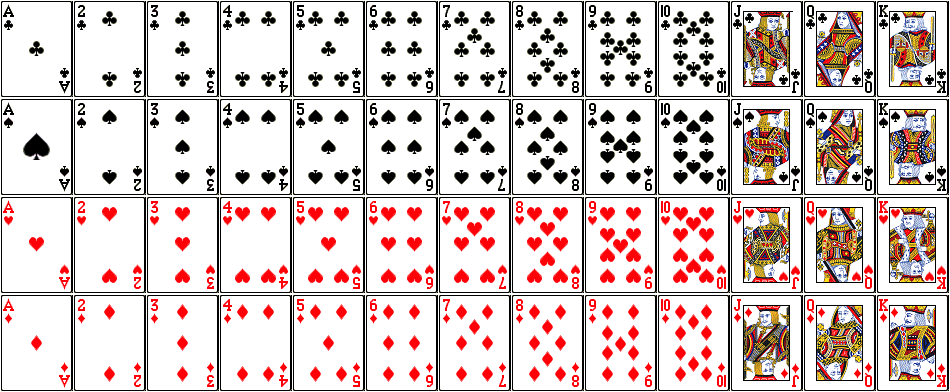
\includegraphics[width=\linewidth]{external/cards.png}
\end{image}%
\tcblower
\end{figureptx}%
\begin{divisionexercise}{5}{}{}{exercise-playing-card-probabilities}%
You are dealt one card from a standard deck of playing cards. Find the probability of being dealt each of the following:%
\begin{enumerate}[label={\alph*}]
\item{}An ace%
\item{}A spade%
\item{}An even heart%
\item{}A face card%
\end{enumerate}
%
\par\smallskip%
\noindent\textbf{\blocktitlefont Solution}.\hypertarget{exercise-playing-card-probabilities-2}{}\quad{}Since there are \(52\) possible cards to be dealt, the total number of outcomes in the sample space is \(n = 52\).%
\par
%
\begin{enumerate}[label={\alph*}]
\item{}There are four possible aces in the deck (one of each suit), so \(m = 4\). Thus,%
\begin{equation*}
P(\text{Ace}) = \frac{4}{52} = \frac{1}{13}
\end{equation*}
%
\item{}There are \(13\) spades in the deck, so \(m = 13\). Thus,%
\begin{equation*}
P(\text{Spade}) = \frac{13}{52} = \frac{1}{4}
\end{equation*}
%
\item{}There are \(5\) even hearts; namely, the 2, 4, 6, 8, and 10 of hearts. So \(m = 5\) and%
\begin{equation*}
P(\text{Even Heart}) = \frac{5}{52}
\end{equation*}
%
\item{}There are \(12\) face cards—the Jack, Queen, and King in each of the four suits—so \(m = 12\). Thus,%
\begin{equation*}
P(\text{Face Card}) = \frac{12}{52} = \frac{3}{13}
\end{equation*}
%
\end{enumerate}
%
\end{divisionexercise}%
\clearpage
\begin{divisionexercise}{6}{}{}{handout-intro-probability-7-1}%
You are dealt one card from a standard deck of \(\displaystyle{52}\) playing cards. Find the probability of being dealt the following.%
\par
(a)  A black card%
\par
\fillintext{20}  %
\par
(b)  An odd diamond  (Note: We are only considering the number cards 2 through 10 as being odd; do NOT count the Ace.)%
\par
\fillintext{20}  %
\par
(c)  The \(\displaystyle{5}\) of spades%
\par
\fillintext{20}  %
\par
(d)  A red face card%
\par
\fillintext{20}  %
\par\smallskip%
\noindent\textbf{\blocktitlefont Answer}.\hypertarget{handout-intro-probability-7-1-2}{}\quad{}%
\begin{itemize}[label=\ptxlistdisc]
\item{}\(\displaystyle \displaystyle\frac{{1}}{{2}}\)%
\item{}\(\displaystyle \displaystyle\frac{{1}}{{13}}\)%
\item{}\(\displaystyle \displaystyle\frac{{1}}{{52}}\)%
\item{}\(\displaystyle \displaystyle\frac{{3}}{{26}}\)%
\end{itemize}
%
\end{divisionexercise}%
\clearpage
Tree diagram for three coin tosses as referred to in \hyperref[fig-coin-toss-tree-clean]{Figure~{\xreffont\ref{fig-coin-toss-tree-clean}}}.%
\begin{divisionexercise}{7}{}{}{handout-intro-probability-8-2}%
\end{divisionexercise}%
\clearpage
\begin{divisionexercise}{8}{}{}{handout-intro-probability-9-1}%
The sample space is shown in \hyperref[table-dice-sample-space]{Table~{\xreffont\ref{table-dice-sample-space}}}.%
\end{divisionexercise}%
\end{worksheet-section}
\restoregeometry
%
%
\typeout{************************************************}
\typeout{Worksheet  09. Activity Probability Events: Not, Or}
\typeout{************************************************}
%
\newgeometry{left=0.75in, right=0.75in, top=0.75in, bottom=0.75in}
\begin{worksheet-section}{Worksheet}{09. Activity Probability Events: Not, Or}{}{09. Activity Probability Events: Not, Or}{}{}{handout-not-or-probability}
Given an experiment with a sample space \(S\), we know how to calculate the probability that an event \(E\) will happen:%
\begin{equation*}
P(E) = \frac{\text{number of outcomes in } E}{\text{total number of outcomes in } S}
\end{equation*}
For example, if we roll a standard 6-sided die, the probability of rolling a 3 is \(\frac{1}{6}\) since there is only one way to roll a 3 and six total outcomes from the roll.%
\par
Now let us examine the probability that an event does \terminology{NOT} happen. Suppose we want to find the probability that we do \terminology{NOT} roll a 3. There are five outcomes in which we do not roll a 3 (namely, 1, 2, 4, 5, and 6), so the probability is \(\frac{5}{6}\). Notice that:%
\begin{equation*}
\frac{1}{6} + \frac{5}{6} = 1
\end{equation*}
This is not a coincidence. Consider a generic situation with \(n\) possible outcomes and an event \(E\) that corresponds to \(m\) of these outcomes. Then the remaining \(n - m\) outcomes correspond to \(E\) not happening, thus:%
\begin{equation*}
P(\text{not } E) = \frac{n - m}{n} = \frac{n}{n} - \frac{m}{n} = 1 - P(E)
\end{equation*}
%
\begin{definition}{Definition}{}{def-complement-event}%
The \terminology{complement} of an event \(E\) is the event \textquotedblleft{}\(E\) does not happen.\textquotedblright{} This is sometimes denoted by \(E^c\) (or \(E'\), \(\overline{E}\)).%
\par
The probability of the complement of \(E\) is calculated using the formula:%
\begin{equation*}
P(E^c) = 1 - P(E)
\end{equation*}
%
\end{definition}
\begin{example}{Example}{}{ex-complement-heart-card}%
You draw a random card from a deck of playing cards. What is the probability that it is not a heart?%
\par\smallskip%
\noindent\textbf{\blocktitlefont Solution}.\hypertarget{ex-complement-heart-card-2}{}\quad{}There are 13 hearts in a deck of 52 cards, so the probability of drawing a heart is:%
\begin{equation*}
P(\text{Heart}) = \frac{13}{52} = \frac{1}{4}
\end{equation*}
Using the complement formula above, the probability that the card is not a heart is:%
\begin{equation*}
P(\text{not Heart}) = 1 - P(\text{Heart}) = 1 - \frac{1}{4} = \frac{3}{4}
\end{equation*}
%
\end{example}
\clearpage
\begin{divisionexercise}{1}{}{}{handout-not-or-probability-3-1}%
Suppose \(\displaystyle{E}\) is an event and \(\displaystyle{P}{\left({E}\right)}=\frac{{3}}{{10}}\). What is \(\displaystyle{P}{\left(\text{not }\ {E}\right)}\)?%
\par
\fillintext{20}  %
\par\smallskip%
\noindent\textbf{\blocktitlefont Answer}.\hypertarget{handout-not-or-probability-3-1-2}{}\quad{}%
\begin{itemize}[label=\ptxlistdisc]
\item{}\(\displaystyle \displaystyle\frac{{7}}{{10}}\)%
\end{itemize}
%
\end{divisionexercise}%
\begin{divisionexercise}{2}{}{}{handout-not-or-probability-3-2}%
You draw a random card from a deck of playing cards.%
\par
What is the probability it is not a queen?%
\par
\fillintext{20}  %
\par
What is the probability that it is not a face card?%
\par
\fillintext{20}  %
\par\smallskip%
\noindent\textbf{\blocktitlefont Answer}.\hypertarget{handout-not-or-probability-3-2-2}{}\quad{}%
\begin{itemize}[label=\ptxlistdisc]
\item{}\(\displaystyle \displaystyle\frac{{12}}{{13}}\)%
\item{}\(\displaystyle \displaystyle\frac{{10}}{{13}}\)%
\end{itemize}
%
\end{divisionexercise}%
\clearpage
Our previous examples have looked at a single event occurring. Now we will look at the probability of one of two events occurring; that is, we will consider the probability of \(A\) or \(B\) occurring, where \(A\) and \(B\) are two different events associated with the experiment being performed. Let us consider an example to demonstrate how to deal with such events.%
\begin{example}{Example}{}{ex-coin-and-die-or}%
Suppose we flipped a coin and rolled a die, and wanted to know the probability of getting a head on the coin \terminology{or} a 6 on the die.%
\par\smallskip%
\noindent\textbf{\blocktitlefont Solution}.\hypertarget{ex-coin-and-die-or-2}{}\quad{}There are \(12\) possible outcomes for this experiment:%
\begin{equation*}
S = \{(H,1), (H,2), (H,3), (H,4), (H,5), (H,6), (T,1), (T,2), (T,3), (T,4), (T,5), (T,6)\}
\end{equation*}
By simply counting, we can see that \(7\) of the outcomes have a head on the coin or a 6 on the die or both; we use \textquotedblleft{}or\textquotedblright{} inclusively here. These outcomes are \((H,1), (H,2), (H,3), (H,4), (H,5), (H,6),\) and \((T,6)\), so the probability is \(\frac{7}{12}\).%
\par
How could we have found this from the individual probabilities? As we would expect, \(6\) of these outcomes have a head, and \(2\) of these outcomes have a 6 on the die. If we add these individual counts, we get \(\frac{6}{12} + \frac{2}{12} = \frac{8}{12}\), which is not the correct probability.%
\par
Looking at the outcomes we can see why: the outcome \((H,6)\) would have been counted twice, since it contains both a head and a 6. The probability of getting both a head and rolling a 6 is \(\frac{1}{12}\). If we subtract out this double count, we have the correct probability:%
\begin{equation*}
\frac{6}{12} + \frac{2}{12} - \frac{1}{12} = \frac{7}{12}
\end{equation*}
%
\end{example}
The above example demonstrates how to compute the probability of an \textquotedblleft{}or\textquotedblright{} event. We state the formula formally now.%
\begin{definition}{Definition}{}{def-probability-or-rule}%
If \(A\) and \(B\) are two events, then the probability of \terminology{\(A\) or \(B\)} (also written as \(A \cup B\)) is given by:%
\begin{equation*}
P(A \text{ or } B) = P(A) + P(B) - P(A \text{ and } B)
\end{equation*}
%
\end{definition}
We consider another example involving cards.%
\begin{example}{Example}{}{ex-card-probabilities-or}%
Suppose we draw one card from a standard deck.%
\begin{enumerate}[label={\alph*}]
\item{}What is the probability that we get a Queen or a King?%
\item{}What is the probability that we get a red card or a King?%
\end{enumerate}
%
\par\smallskip%
\noindent\textbf{\blocktitlefont Solution}.\hypertarget{ex-card-probabilities-or-2}{}\quad{}We know there are \(52\) possible cards, so \(n = 52\).%
\par
%
\begin{enumerate}[label={\alph*}]
\item{}There are \(4\) Queens and \(4\) Kings in the deck, so \(P(\text{Queen}) = \frac{4}{52}\) and \(P(\text{King}) = \frac{4}{52}\). There are no cards which are both a Queen and a King, so \(P(\text{Queen and King}) = \frac{0}{52} = 0\). Thus,%
\begin{equation*}
P(\text{Queen or King}) = \frac{4}{52} + \frac{4}{52} - 0 = \frac{8}{52} = \frac{2}{13}
\end{equation*}
%
\item{}There are \(26\) red cards and \(4\) Kings in the deck, so \(P(\text{Red}) = \frac{26}{52}\) and \(P(\text{King}) = \frac{4}{52}\). There are \(2\) cards which are both red and a King (the King of Hearts and King of Diamonds), so \(P(\text{Red and King}) = \frac{2}{52}\). Thus,%
\begin{equation*}
P(\text{Red or King}) = \frac{26}{52} + \frac{4}{52} - \frac{2}{52} = \frac{28}{52} = \frac{7}{13}
\end{equation*}
%
\end{enumerate}
%
\end{example}
\begin{note}{Note}{}{note-reducing-fractions}%
Note that it was advantageous in the previous example to wait until the final calculation to reduce the fractions. This allows us to easily add fractions with a common denominator—in this case, \(52\)—and reduce the answer once.%
\end{note}
\begin{divisionexercise}{3}{}{}{handout-not-or-probability-4-8}%
Suppose we flipped a coin and rolled a die. What is the probability of getting a tail on the coin or an even number on the die?%
\par
\fillintext{20}  %
\par\smallskip%
\noindent\textbf{\blocktitlefont Answer}.\hypertarget{handout-not-or-probability-4-8-2}{}\quad{}%
\begin{itemize}[label=\ptxlistdisc]
\item{}\(\displaystyle \displaystyle\frac{{3}}{{4}}\)%
\end{itemize}
%
\end{divisionexercise}%
\begin{divisionexercise}{4}{}{}{handout-not-or-probability-4-9}%
Suppose we draw one card from a standard deck.%
\par
(a) What is the probability that we get a spade or a heart?%
\par
\fillintext{20}  %
\par
(b) What is the probability that we get a spade or a face card?%
\par
\fillintext{20}  %
\par\smallskip%
\noindent\textbf{\blocktitlefont Answer}.\hypertarget{handout-not-or-probability-4-9-2}{}\quad{}%
\begin{itemize}[label=\ptxlistdisc]
\item{}\(\displaystyle \displaystyle\frac{{1}}{{2}}\)%
\item{}\(\displaystyle \displaystyle\frac{{11}}{{26}}\)%
\end{itemize}
%
\end{divisionexercise}%
\clearpage
We consider one additional example with information presented using a table. The table below shows the number of survey subjects who have received and not received a speeding ticket in the last year, and the color of their car.%
\begin{tableptx}{Table}{\textbf{}}{table-speeding-tickets}{}%
\centering%
{\tabularfont%
\begin{tabular}{AlAlAlAlA}\hrulethin
{\bfseries{}}&{\bfseries{}Speeding ticket}&{\bfseries{}No speeding ticket}&{\bfseries{}Total}\tabularnewline\hrulethin
Red car&15&135&150\tabularnewline\hrulethin
Not red car&45&470&515\tabularnewline\hrulethin
Total&60&605&665\tabularnewline\hrulethin
\end{tabular}
}%
\end{tableptx}%
\begin{example}{Example}{}{ex-speeding-ticket-probabilities}%
Find the probability that a randomly chosen person:%
\begin{enumerate}[label={\alph*)}]
\item{}has a red car \terminology{and} got a speeding ticket%
\item{}has a red car \terminology{or} got a speeding ticket%
\end{enumerate}
%
\par\smallskip%
\noindent\textbf{\blocktitlefont Solution}.\hypertarget{ex-speeding-ticket-probabilities-2}{}\quad{}The total number of people surveyed is \(n = 665\).%
\par
%
\begin{enumerate}[label={\alph*)}]
\item{}From the table, we can see that \(15\) of the people surveyed had a red car and got a speeding ticket, so \(m = 15\). Thus,%
\begin{equation*}
P(\text{Red Car and Ticket}) = \frac{15}{665} = \frac{3}{133}
\end{equation*}
%
\item{}From the table, we can see that \(150\) people have a red car, \(60\) people got a speeding ticket, and \(15\) people have a red car and got a speeding ticket. Using the addition rule to account for the double count, we find the number of favorable outcomes is \(150 + 60 - 15 = 195\). Thus,%
\begin{equation*}
P(\text{Red Car or Ticket}) = \frac{150}{665} + \frac{60}{665} - \frac{15}{665} = \frac{195}{665} = \frac{39}{133}
\end{equation*}
%
\end{enumerate}
%
\end{example}
\begin{divisionexercise}{5}{}{}{handout-not-or-probability-5-4}%
Using the table above, find the probability that a randomly choosen person:%
\par
(a)  does not have a red car and did not get a speeding ticket.%
\par
\fillintext{20}  %
\par
(b) does not have a red can or did not get a speeding ticket.%
\par
\fillintext{20}  %
\par\smallskip%
\noindent\textbf{\blocktitlefont Answer}.\hypertarget{handout-not-or-probability-5-4-2}{}\quad{}%
\begin{itemize}[label=\ptxlistdisc]
\item{}\(\displaystyle \displaystyle\frac{{470}}{{665}}\)%
\item{}\(\displaystyle \displaystyle\frac{{650}}{{665}}\)%
\end{itemize}
%
\end{divisionexercise}%
\end{worksheet-section}
\restoregeometry
%
%
\typeout{************************************************}
\typeout{Worksheet  10. Activity The Fundamental Counting Principle}
\typeout{************************************************}
%
\newgeometry{left=0.75in, right=0.75in, top=0.75in, bottom=0.75in}
\begin{worksheet-section}{Worksheet}{10. Activity The Fundamental Counting Principle}{}{10. Activity The Fundamental Counting Principle}{}{}{handout-FCP}
All of the probability problems we encountered in the previous unit had a relatively small sample space. Many situations involve very large sample spaces which cannot be written down, e.g., the number of \(8\)-character passwords for a computer. For these types of situations, we need an efficient way to count certain types of items. We will ultimately use three primary counting tools: the Fundamental Counting Principle, Permutations, and Combinations. We discuss the first two of these in this activity.%
\par
Let's begin with a real-life situation. Suppose you are at a restaurant, and the menu has three choices for an appetizer (soup, salad, or breadsticks) and five choices for a main course (hamburger, sandwich, quiche, fajita, or pizza). You are allowed to choose exactly one appetizer and one main course for your meal. How many different options do you have?%
\par
There are different approaches to solving this problem. One possible approach is to list all possible meals. Here is an attempt to do so:%
\begin{itemize}[label=\ptxlistdisc]
\item{}Soup + hamburger%
\item{}Soup + fajita%
\item{}Salad + pizza%
\item{}Salad + hamburger%
\item{}Breadsticks + sandwich%
\item{}Breadsticks + quiche%
\item{}Salad + fajita%
\item{}Salad + quiche%
\item{}Salad + sandwich%
\item{}Soup + sandwich%
\item{}Soup + pizza%
\item{}Soup + quiche%
\item{}Breadsticks + pizza%
\item{}Breadsticks + hamburger%
\end{itemize}
This list suggests there are \(14\) different options, but does this list include all of them? This is an issue with this particular approach; in order to know the number of meals possible, we must ensure that all options have been accounted for in our list. In this case, I intentionally left one out; the astute reader will notice Breadsticks + fajita does not appear in the above list.%
\par
Another approach is to make a table with rows for each appetizer and columns for each main course.%
\clearpage
\begin{tableptx}{Table}{\textbf{}}{table-menu-options}{}%
\centering%
{\tabularfont%
\begin{tabular}{AlAlAlAlAlAlA}\hrulethin
{\bfseries{}}&{\bfseries{}Hamburger}&{\bfseries{}Sandwich}&{\bfseries{}Quiche}&{\bfseries{}Fajita}&{\bfseries{}Pizza}\tabularnewline\hrulethin
Soup&1&2&3&4&5\tabularnewline\hrulethin
Salad&6&7&8&9&10\tabularnewline\hrulethin
Breadsticks&11&12&13&14&15\tabularnewline\hrulethin
\end{tabular}
}%
\end{tableptx}%
This tabular approach ensures we have all the options included! Counting the number of cells in the table shows there are \(15\) options at the restaurant. Moreover, from this approach we can see exactly how to calculate the total number of options based on the number of appetizers and the number of main courses: since there are \(3\) rows (corresponding to the appetizers) and \(5\) columns (corresponding to the main courses), we can see the number of options is \(3 \times 5 = 15\). This demonstrates what we will refer to as the Fundamental Counting Principle.%
\begin{definition}{Definition}{}{def-fundamental-counting-principle}%
\index{Fundamental Counting Principle} If we are asked to choose one item from each of two separate categories where there are \(m\) items in the first category and \(n\) items in the second category, then the total number of available choices is:%
\begin{equation*}
m \times n
\end{equation*}
%
\end{definition}
\begin{example}{Example}{}{ex-reading-list-combinations}%
There are \(8\) novels and \(5\) volumes of poetry on a reading list for a college English course. How many different ways can a student select one novel and one volume of poetry to read for the course?%
\par\smallskip%
\noindent\textbf{\blocktitlefont Solution}.\hypertarget{ex-reading-list-combinations-2}{}\quad{}There are two categories here: novels and volumes of poetry. By the Fundamental Counting Principle, the number of ways to choose one item from each of the two categories is:%
\begin{equation*}
8 \times 5 = 40
\end{equation*}
%
\end{example}
\begin{divisionexercise}{1}{}{}{handout-FCP-3-5}%
Which of the following counting techniques will we discuss in class. Select ALL that apply!%
\par
%
\begin{enumerate}[label={(\alph*)}]
\item{}Pigeonhole Principle%
\item{}Fundamental Counting Principle%
\item{}Combinations%
\item{}Conditional Counting Principle%
\item{}Permutations%
\item{}Inclusion-Exclusion Principle%
\end{enumerate}
%
\par\smallskip%
\noindent\textbf{\blocktitlefont Answer}.\hypertarget{handout-FCP-3-5-2}{}\quad{}%
\begin{itemize}[label=\ptxlistdisc]
\item{}Fundamental Counting Principle%
\par
Permutations%
\par
Combinations%
\end{itemize}
%
\end{divisionexercise}%
\clearpage
\begin{divisionexercise}{2}{}{}{handout-FCP-4-1}%
Use the Fundamental Counting Principle to answer the following questions.%
\par
A restaurant offers \(\displaystyle{15}\) appetizers and \(\displaystyle{10}\) main courses. In how many different ways can a person order a two-course meal?%
\par
\fillintext{20}%
\par
A college student needs to take a psychology course and an economics course during the summer session. There are \(\displaystyle{12}\) options for a psychology course and \(\displaystyle{9}\) options for an economics course. How many possible summer schedules does this student have to choose from?%
\par
\fillintext{20}%
\par
You are buying a new car. There are \(\displaystyle{17}\) possible colors to choose from and you have the option of either manual or automatic transmission. How many different car options do you have?%
\par
\fillintext{20}%
\par\smallskip%
\noindent\textbf{\blocktitlefont Answer}.\hypertarget{handout-FCP-4-1-2}{}\quad{}%
\begin{itemize}[label=\ptxlistdisc]
\item{}150%
\item{}108%
\item{}34%
\end{itemize}
%
\end{divisionexercise}%
\clearpage
The Fundamental Counting Principle can be extended when there are more than two categories by applying it repeatedly. Here are some examples of this.%
\begin{example}{Example}{}{ex-pizza-combinations}%
A pizza shop has a special promotion which allows you to buy a one-topping pizza at half price! They offer three different sizes, four different crusts, and twelve different topping options. How many different pizzas can be purchased under this promotion?%
\par\smallskip%
\noindent\textbf{\blocktitlefont Solution}.\hypertarget{ex-pizza-combinations-2}{}\quad{}There are three different categories here (size, crust, topping) from which we need to choose one option each. By the Fundamental Counting Principle, the total number of pizzas which can be purchased is:%
\begin{equation*}
3 \times 4 \times 12 = 144
\end{equation*}
%
\end{example}
\begin{example}{Example}{}{ex-true-false-quiz}%
A quiz consists of five true-or-false questions. In how many ways can a student answer the quiz?%
\par\smallskip%
\noindent\textbf{\blocktitlefont Solution}.\hypertarget{ex-true-false-quiz-2}{}\quad{}In this scenario the categories are the questions on the quiz; we need to choose an answer for each of the five questions. Each question has \(2\) possible answers, either \textquotedblleft{}True\textquotedblright{} or \textquotedblleft{}False\textquotedblright{}. This means we have \(2\) possible choices in each of the five categories, so the total number of ways to answer the quiz is:%
\begin{equation*}
2 \times 2 \times 2 \times 2 \times 2 = 32
\end{equation*}
Note this can be written as \(2^5 = 32\). This can be a useful way to write this answer!%
\end{example}
\begin{example}{Example}{}{ex-telephone-counting}%
A telephone number consists of a \(3\)-digit area code followed by a \(7\)-digit local phone number. Area codes and local phone numbers cannot begin with a \(0\) or \(1\). How many different phone numbers are possible?%
\par\smallskip%
\noindent\textbf{\blocktitlefont Solution}.\hypertarget{ex-telephone-counting-2}{}\quad{}One way to think about a problem like this is to use what can be called a \textquotedblleft{}blank diagram\textquotedblright{}. A blank diagram will show a blank space for each item that needs to be chosen, and then we can fill in each blank with the number of choices we have for that item. For this particular scenario, a blank diagram might look like this, modeled after how we traditionally write phone numbers:%
\begin{equation*}
(\underline{\quad} \ \underline{\quad} \ \underline{\quad}) \ \underline{\quad} \ \underline{\quad} \ \underline{\quad} - \underline{\quad} \ \underline{\quad} \ \underline{\quad} \ \underline{\quad}
\end{equation*}
%
\par
We start on the left side and fill in one blank at a time with the number of options we have for that position. The left-most number is the first digit in the area code. We are told this cannot be \(0\) or \(1\), which means it can be any of the digits \(2, 3, 4, 5, 6, 7, 8,\) or \(9\). There are \(8\) possible options here, so we fill in the first blank with an \(8\):%
\begin{equation*}
(\underline{8} \ \underline{\quad} \ \underline{\quad}) \ \underline{\quad} \ \underline{\quad} \ \underline{\quad} - \underline{\quad} \ \underline{\quad} \ \underline{\quad} \ \underline{\quad}
\end{equation*}
%
\par
The next number can be any digit; we have no restriction on the second digit of the area code. So we can fill in the second blank with the total number of options for that digit (the digits \(0\) through \(9\), which gives \(10\) choices):%
\begin{equation*}
(\underline{8} \ \underline{10} \ \underline{\quad}) \ \underline{\quad} \ \underline{\quad} \ \underline{\quad} - \underline{\quad} \ \underline{\quad} \ \underline{\quad} \ \underline{\quad}
\end{equation*}
%
\par
Similarly, there are \(10\) options for the third digit of the area code:%
\begin{equation*}
(\underline{8} \ \underline{10} \ \underline{10}) \ \underline{\quad} \ \underline{\quad} \ \underline{\quad} - \underline{\quad} \ \underline{\quad} \ \underline{\quad} \ \underline{\quad}
\end{equation*}
%
\par
Like with the area code, the first digit of the local phone number cannot be \(0\) or \(1\), so we have \(8\) possible choices. The remaining digits have no restriction, so they can be any of the \(10\) possible digits:%
\begin{equation*}
(\underline{8} \ \underline{10} \ \underline{10}) \ \underline{8} \ \underline{10} \ \underline{10} - \underline{10} \ \underline{10} \ \underline{10} \ \underline{10}
\end{equation*}
%
\par
Once we have filled in all the blanks, we can multiply the number of options together to form the total number of possible phone numbers:%
\begin{equation*}
8 \times 10 \times 10 \times 8 \times 10 \times 10 \times 10 \times 10 \times 10 \times 10 = 6,400,000,000
\end{equation*}
%
\end{example}
\clearpage
\begin{divisionexercise}{3}{}{}{handout-FCP-6-1}%
Answer the following questions using the Fundamental Couting Principle.%
\par
At a particular restaurant you have eight choices for an appetizer, eleven choices for a main course, and five choices for a desert. If you are allowed to choose exactly one item from each category, how many different meal options do you have?%
\par
\fillintext{20}%
\par
You are purchasing a new car. You can choose from \(\displaystyle{9}\) different colors, with or without air conditioning, electric or gas powered, and with or without a satellite radio. How many different car selections are possible?%
\par
\fillintext{20}%
\par\smallskip%
\noindent\textbf{\blocktitlefont Answer}.\hypertarget{handout-FCP-6-1-2}{}\quad{}%
\begin{itemize}[label=\ptxlistdisc]
\item{}440%
\item{}72%
\end{itemize}
%
\end{divisionexercise}%
\begin{divisionexercise}{4}{}{}{handout-FCP-6-2}%
A company puts a code on each product they sell. The code is made up of three digits followed by two letters (\(\displaystyle{a}\) through \(\displaystyle{z}\), not case specific). For example, \(\displaystyle{123}{a}{z}\), \(\displaystyle{788}{c}{d}\), and \(\displaystyle{010}{j}{k}\) are all possible product codes. How many different codes are possible?%
\par
\fillintext{20}%
\par\smallskip%
\noindent\textbf{\blocktitlefont Answer}.\hypertarget{handout-FCP-6-2-2}{}\quad{}%
\begin{itemize}[label=\ptxlistdisc]
\item{}676000%
\end{itemize}
%
\end{divisionexercise}%
\end{worksheet-section}
\restoregeometry
%
%
\typeout{************************************************}
\typeout{Worksheet  11. Activity Permutations}
\typeout{************************************************}
%
\newgeometry{left=0.75in, right=0.75in, top=0.75in, bottom=0.75in}
\begin{worksheet-section}{Worksheet}{11. Activity Permutations}{}{11. Activity Permutations}{}{}{handout-Permutations}
Let's now consider a slightly different counting problem.%
\begin{example}{Example}{}{ex-word-rearrangement}%
How many different ways can the letters of the word \(\text{MATH}\) be rearranged to form a four-letter code word? (E.g., \(\text{MATH}\), \(\text{AMTH}\), \(\text{HTAM}\), etc.)%
\par\smallskip%
\noindent\textbf{\blocktitlefont Solution}.\hypertarget{ex-word-rearrangement-2}{}\quad{}We can use a blank diagram to help us answer this question! We start with one with four blanks, one for each of the positions in the code word:%
\begin{equation*}
\underline{\quad} \ \underline{\quad} \ \underline{\quad} \ \underline{\quad}
\end{equation*}
%
\par
There are \(4\) choices for the first letter of the code word; it can be \(\text{M}\) \(\text{A}\), \(\text{T}\), or \(\text{H}\). Thus, we have:%
\begin{equation*}
\underline{4} \ \underline{\quad} \ \underline{\quad} \ \underline{\quad}
\end{equation*}
%
\par
Once the first letter is chosen, there are only \(3\) choices for the second letter of the code word. For example, if \(\text{M}\) is chosen as the first letter, then the options for the second are \(\text{A}\), \(\text{T}\), and \(\text{H}\), since \(\text{M}\) cannot be used a second time. Or, if \(\text{A}\) is chosen as the first letter, then the options for the second are \(\text{M}\), \(\text{T}\), and \(\text{H}\). The key is that regardless of the choice for the first letter, there will always be \(3\) options to choose from for the second letter. So:%
\begin{equation*}
\underline{4} \ \underline{3} \ \underline{\quad} \ \underline{\quad}
\end{equation*}
%
\par
Using a similar logic, once the first two letters are chosen there are only \(2\) options remaining for the third letter. For example, if \(\text{M}\) is chosen first and \(\text{A}\) chosen second, then the options for the third letter are only \(\text{T}\) and \(\text{H}\). Thus:%
\begin{equation*}
\underline{4} \ \underline{3} \ \underline{2} \ \underline{\quad}
\end{equation*}
%
\par
Finally, there is only \(1\) choice for the final letter, since all of the other letters have been used at this point. This means our completed blank diagram looks like:%
\begin{equation*}
\underline{4} \ \underline{3} \ \underline{2} \ \underline{1}
\end{equation*}
%
\par
So by the Fundamental Counting Principle, the number of code words is:%
\begin{equation*}
4 \times 3 \times 2 \times 1 = 24
\end{equation*}
%
\end{example}
This is a simple example of what is called a \terminology{permutation}. A permutation is an ordered arrangement of items that occurs when:%
\begin{itemize}[label=\ptxlistdisc]
\item{}No item is used more than once, and%
\item{}The order of arrangement makes a difference (e.g., \(\text{MA}\) is different than \(\text{AM}\)).%
\end{itemize}
%
\par
The product that we saw in the preceding example is called a \terminology{factorial} and is denoted \(n!\). In general, \(n!\) is read as \textquotedblleft{}\(n\) factorial.\textquotedblright{} For example:%
\begin{equation*}
4! = 4 \times 3 \times 2 \times 1 = 24
\end{equation*}
%
\begin{definition}{Definition}{}{def-factorial-permutations}%
\index{factorial}\index{permutation} When a situation involves rearranging all of the objects in a given set, then the number of permutations is given by:%
\begin{equation*}
n! = n \times (n-1) \times (n-2) \times \dots \times 3 \times 2 \times 1
\end{equation*}
where \(n\) is the total number of objects.%
\end{definition}
\begin{note}{Note}{}{note-calculator-factorial}%
Scientific calculators have a button which will compute factorials automatically. If you have the TI-30XIIS calculator, you can access this by hitting the \kbd{PRB} button and arrowing over to the \(!\) symbol.%
\end{note}
\begin{example}{Example}{}{ex-door-prizes}%
How many ways can five different door prizes be distributed among five people?%
\par\smallskip%
\noindent\textbf{\blocktitlefont Solution}.\hypertarget{ex-door-prizes-2}{}\quad{}Here we want to rearrange the five people in order so that the first gets the first prize, the second gets the second prize, and so on. We must rearrange all five of the people since there are five prizes, so the number of ways to do this is:%
\begin{equation*}
5! = 5 \times 4 \times 3 \times 2 \times 1 = 120
\end{equation*}
%
\end{example}
\clearpage
\begin{divisionexercise}{1}{}{}{handout-Permutations-3-1}%
Answer the following questions. Feel free to use the factorial key on your calculator to find the answers.%
\par
In how many different ways can a police department arrange \(\displaystyle{8}\) suspects in a police lineup if each lineup contains all eight people?%
\par
\fillintext{20}%
\par
Twelve friends want to sit together at a movie theater. Conveniently, one of the rows has exactly \(\displaystyle{12}\) seats. How many different seating arrangements are possible?%
\par
\fillintext{20}%
\par\smallskip%
\noindent\textbf{\blocktitlefont Answer}.\hypertarget{handout-Permutations-3-1-2}{}\quad{}%
\begin{itemize}[label=\ptxlistdisc]
\item{}40320%
\item{}479001600%
\end{itemize}
%
\end{divisionexercise}%
\clearpage
Sometimes there are scenarios where we want to determine the number of ways to rearrange only a subset of a set of objects. The next two examples present two such scenarios.%
\begin{example}{Example}{}{ex-gift-certificates}%
A charity benefit is attended by \(25\) people and three gift certificates are given away as door prizes: one gift certificate is in the amount of \(\$100\), the second is worth \(\$25\), and the third is worth \(\$10\). Assuming that no person receives more than one prize, how many different ways can the three gift certificates be awarded?%
\par\smallskip%
\noindent\textbf{\blocktitlefont Solution}.\hypertarget{ex-gift-certificates-2}{}\quad{}Since the three gift certificates are worth different amounts, the order in which they are awarded makes a difference. There are \(25\) possible winners for the \(\$100\) gift certificate. Once that has been awarded, there are \(24\) possible winners for the \(\$25\) gift certificate since the first winner is not eligible. Finally, after the first two have been awarded there are \(23\) possible winners for the \(\$10\) gift certificate since the first two winners are ineligible. The total number of ways the three gift certificates can be awarded is:%
\begin{equation*}
25 \times 24 \times 23 = 13,800
\end{equation*}
%
\end{example}
\begin{example}{Example}{}{ex-olympic-sprinters}%
Eight sprinters have made it to the Olympic finals in the 100-meter race. In how many different ways can the gold, silver, and bronze medals be awarded?%
\par\smallskip%
\noindent\textbf{\blocktitlefont Solution}.\hypertarget{ex-olympic-sprinters-2}{}\quad{}Like the previous example, the order in which the medals are awarded makes a difference since they are different. There are \(8\) possible gold medalists, then \(7\) possible silver medalists (the runner who wins gold cannot win silver), and finally \(6\) possible bronze medalists (the gold and silver medalists cannot win bronze). This means the number of ways the medals can be awarded is:%
\begin{equation*}
8 \times 7 \times 6 = 336
\end{equation*}
%
\end{example}
The two examples above are similar in that:%
\begin{itemize}[label=\ptxlistdisc]
\item{}They had a total group of people (\(25\) and \(8\), respectively) and wanted to order a strictly smaller number of them (in both cases, \(3\)).%
\item{}The order of selection was important (e.g., first place, second place, third place).%
\item{}Awards were done without replacement; whoever was chosen first could not be chosen again.%
\end{itemize}
These examples demonstrate permutations where only a select number of items are chosen to be rearranged.%
\par
Here is the general scenario. Suppose we have \(n\) total objects and want to choose \(r\) of them without replacement when order matters (this is what was done in the preceding examples!). The number of ways this can be done is denoted \(_nP_r\) and is given by the formula:%
\begin{equation*}
_nP_r = \frac{n!}{(n-r)!}
\end{equation*}
%
\begin{note}{Note}{}{note-calculator-npr}%
Your calculator should have a key to calculate this for you! If you are using the TI-30XIIS, the key is located in the \kbd{PRB} menu along with the factorial key!%
\end{note}
\clearpage
\begin{example}{Example}{}{ex-painting-arrangements}%
Bo has nine paintings and has room to display only four of them at a time on his wall. How many different ways could Bo do this?%
\par\smallskip%
\noindent\textbf{\blocktitlefont Solution}.\hypertarget{ex-painting-arrangements-2}{}\quad{}In this example, we have a total of \(9\) paintings to choose from and need to choose \(4\) of them. The order of selection matters since they are being arranged on a wall, and none can be used more than once. This is a permutation! Using a calculator to find \(_9P_4\), the number of ways for Bo to arrange four paintings is:%
\begin{equation*}
_9P_4 = \frac{9!}{(9-4)!} = \frac{9!}{5!} = 9 \times 8 \times 7 \times 6 = 3,024
\end{equation*}
%
\end{example}
\begin{example}{Example}{}{ex-executive-committee}%
How many ways can a four-person executive committee (president, vice-president, secretary, treasurer) be selected from a 16-member board of directors of a non-profit organization?%
\par\smallskip%
\noindent\textbf{\blocktitlefont Solution}.\hypertarget{ex-executive-committee-2}{}\quad{}In this example, we have a total of \(16\) people to choose from and need to choose \(4\) of them. The order of selection matters (e.g., being president is different than being secretary), and no one can serve in multiple roles. This is a permutation! Using a calculator to find \(_{16}P_4\), the number of ways to form such a committee is:%
\begin{equation*}
_{16}P_4 = \frac{16!}{(16-4)!} = \frac{16!}{12!} = 16 \times 15 \times 14 \times 13 = 43,680
\end{equation*}
%
\end{example}
\clearpage
\begin{divisionexercise}{2}{}{}{handout-Permutations-6-1}%
Answer the following questions. Use the \(\displaystyle\ _{{n}}{P}_{{r}}\) button on your calculator!%
\par
You are the coach for a little league baseball team. There are \(\displaystyle{13}\) players on the team. You need to choose a batting order having \(\displaystyle{9}\) players. How many different batting orders can you make?%
\par
\fillintext{20}%
\par
A TV network needs to fill up five different time slots and has \(\displaystyle{10}\) classic sitcoms available. In how many ways can they fill these available time slots?%
\par
\fillintext{20}%
\par\smallskip%
\noindent\textbf{\blocktitlefont Answer}.\hypertarget{handout-Permutations-6-1-2}{}\quad{}%
\begin{itemize}[label=\ptxlistdisc]
\item{}259459200%
\item{}30240%
\end{itemize}
%
\end{divisionexercise}%
\begin{divisionexercise}{3}{}{}{handout-Permutations-6-2}%
You need to make a \(\displaystyle{5}\)-character password using the letters \(\displaystyle{A}\) through \(\displaystyle{Z}\).%
\par
How many passwords are possible if repeated letters are allowed?%
\par
\fillintext{20}%
\par
How many passwords are possible if repeated letters are NOT allowed?%
\par
\fillintext{20}%
\par\smallskip%
\noindent\textbf{\blocktitlefont Answer}.\hypertarget{handout-Permutations-6-2-2}{}\quad{}%
\begin{itemize}[label=\ptxlistdisc]
\item{}11881376%
\item{}7893600%
\end{itemize}
%
\end{divisionexercise}%
\end{worksheet-section}
\restoregeometry
%
%
\typeout{************************************************}
\typeout{Worksheet  12. Activity Combinations}
\typeout{************************************************}
%
\newgeometry{left=0.75in, right=0.75in, top=0.75in, bottom=0.75in}
\begin{worksheet-section}{Worksheet}{12. Activity Combinations}{}{12. Activity Combinations}{}{}{handout-Combinations}
Consider the following scenario, which is a slight modification of an example we considered in the previous section. A charity benefit is attended by \(25\) people and three gift certificates are given away as door prizes. Each gift certificate is \(\$100\). Assuming that no person receives more than one prize, how many different ways can the three gift certificates be awarded?%
\par
In the previous example, the three gift certificates were for different amounts and therefore the order the three winners were selected in made a difference. Here, the order in which the three winners are chosen does \terminology{NOT} matter! We only care about which three individuals get the gift certificates since they are the same amount! Essentially, we want the number of ways to choose a group of \(3\) people from the \(25\) attendees.%
\par
This is an example of what is called a \terminology{combination}. Suppose we have \(n\) total objects and want to choose \(r\) of them without replacement when order does not matter. The number of ways this can be done is denoted \(_nC_r\) and is given by the formula:%
\begin{equation*}
_nC_r = \frac{n!}{r!(n-r)!}
\end{equation*}
%
\begin{note}{Note}{}{note-calculator-ncr}%
Your calculator will have a key to calculate the number of combinations directly. If you have the TI-30XIIS, it can be found under the \kbd{PRB} menu along with the factorial (\(!\)) and permutation (\(_nP_r\)) functions.%
\end{note}
To return to the example at the top of this section, we can find the number of ways to award the three gift certificates by using the combination function on a calculator:%
\begin{equation*}
_{25}C_{3} = \frac{25!}{3!(25-3)!} = \frac{25!}{3! \times 22!} = \frac{25 \times 24 \times 23}{3 \times 2 \times 1} = 2,300
\end{equation*}
%
\begin{divisionexercise}{1}{}{}{handout-Combinations-2-6}%
A charity benefit is attended by \(\displaystyle{20}\) people and five gift certificates are given away as door prizes. Each gift certificate is \(\displaystyle\${30}\). Assuming that no person receives more than one prize, how many different ways can the five gift certificates be awarded?%
\par
\fillintext{20}%
\par\smallskip%
\noindent\textbf{\blocktitlefont Answer}.\hypertarget{handout-Combinations-2-6-2}{}\quad{}%
\begin{itemize}[label=\ptxlistdisc]
\item{}15504%
\end{itemize}
%
\end{divisionexercise}%
\clearpage
One key aspect of counting is to be able to distinguish between a permutation and a combination. The main point to consider is whether or not the order in which the items are selected matters. If the order matters, then we need to use permutations; if the order does not matter, we need to use combinations.%
\begin{example}{Example}{}{ex-permutation-vs-combination}%
A class has \(30\) total students.%
\begin{enumerate}[label={\alph*}]
\item{}The class must choose a president, vice president, secretary, and treasurer for the year. In how many ways can this be done?%
\item{}The class must also choose four students to represent the class in the student council. In how many ways can this be done?%
\end{enumerate}
%
\par\smallskip%
\noindent\textbf{\blocktitlefont Solution}.\hypertarget{ex-permutation-vs-combination-2}{}\quad{}%
\begin{enumerate}[label={\alph*}]
\item{}We need to choose four students, and the order makes a difference here because the roles of the students will be different (e.g., being president is different than being treasurer). This is a permutation, so the number of ways this can be done is:%
\begin{equation*}
_{30}P_{4} = \frac{30!}{(30-4)!} = 30 \times 29 \times 28 \times 27 = 657,720
\end{equation*}
%
\item{}In this case, the order in which the students are chosen does not matter; all four chosen students will serve the same role (namely, being a member of the student council). This is a combination, so the number of ways this can be done is:%
\begin{equation*}
_{30}C_{4} = \frac{30!}{4!(30-4)!} = \frac{30 \times 29 \times 28 \times 27}{4 \times 3 \times 2 \times 1} = 27,405
\end{equation*}
%
\end{enumerate}
%
\end{example}
\begin{divisionexercise}{2}{}{}{handout-Combinations-3-3}%
Answer the following questions. Note these are the same questions as in the previous exercise, where you determined whether they were permutations or combinations.%
\par
(a)  In poker, a player is dealt five cards from a standard \(\displaystyle{52}\)-card deck. How many different poker hands are possible?%
\par
\fillintext{20}%
\par
(b)  You volunteer to pet-sit for a friend who has 7 animals. How many different pet combinations are possible if you only have the room to pet-set three animals?%
\par
\fillintext{20}%
\par
(c)  Ten swimmers compete in a race. In how many ways can the first place, second place, and third place medals be awarded?%
\par
\fillintext{20}%
\par
(d)  An election ballot asks voters to select three city commissioners from a group of six candidates. In how many ways can this be done?%
\par
\fillintext{20}%
\par\smallskip%
\noindent\textbf{\blocktitlefont Answer}.\hypertarget{handout-Combinations-3-3-2}{}\quad{}%
\begin{itemize}[label=\ptxlistdisc]
\item{}2598960%
\item{}35%
\item{}720%
\item{}20%
\end{itemize}
%
\end{divisionexercise}%
\clearpage
\begin{divisionexercise}{3}{}{}{handout-Combinations-4-1}%
For each scenario, determine whether the answer would be a permutation or combination.%
\par
(a)  In poker, a player is dealt five cards from a standard \(\displaystyle{52}\)-card deck. How many different poker hands are possible? \textasciigrave{}%
\par
%
\begin{enumerate}[label={(\alph*)}]
\item{}Permutation%
\item{}Combination%
\end{enumerate}
%
\par
(b)  You volunteer to pet-sit for a friend who has 7 animals. How many different pet combinations are possible if you only have the room to pet-set three animals?%
\par
%
\begin{enumerate}[label={(\alph*)}]
\item{}Permutation%
\item{}Combination%
\end{enumerate}
%
\par
(c)  Ten swimmers compete in a race. In how many ways can the first place, second place, and third place medals be awarded?%
\par
%
\begin{enumerate}[label={(\alph*)}]
\item{}Permutation%
\item{}Combination%
\end{enumerate}
%
\par
(d)  An election ballot asks voters to select three city commissioners from a group of six candidates. In how many ways can this be done?%
\par
%
\begin{enumerate}[label={(\alph*)}]
\item{}Permutation%
\item{}Combination%
\end{enumerate}
%
\par\smallskip%
\noindent\textbf{\blocktitlefont Answer}.\hypertarget{handout-Combinations-4-1-2}{}\quad{}%
\begin{itemize}[label=\ptxlistdisc]
\item{}B: Combination%
\item{}B: Combination%
\item{}A: Permutation%
\item{}B: Combination%
\end{itemize}
%
\end{divisionexercise}%
\clearpage
Sometimes combinations must be combined with the Fundamental Counting Principle to solve a problem! Here is an example of this!%
\begin{example}{Example}{}{ex-senate-committees}%
The US Senate of a particular Congress consisted of \(48\) Democrats, \(50\) Republicans, and \(2\) Independents. How many committees can be formed if each committee must have exactly \(3\) Democrats and \(3\) Republicans?%
\par\smallskip%
\noindent\textbf{\blocktitlefont Solution}.\hypertarget{ex-senate-committees-2}{}\quad{}To answer this question, we need to break the problem down into three steps:%
\begin{enumerate}[label={(\alph*)}]
\item{}Determine the number of ways to choose the Democrats from the possible Democrats.%
\item{}Determine the number of ways to choose the Republicans from the possible Republicans.%
\item{}Use the numbers determined in the first two steps to count the total number of possible committees.%
\end{enumerate}
%
\par
For steps 1 and 2, note that the order in which we choose the Democrats and Republicans does not matter; all we care about is the set of people chosen from each party. Since the order does not matter, the number of ways to choose \(3\) Democrats from the total of \(48\) Democrats is:%
\begin{equation*}
_{48}C_{3} = \frac{48!}{3!(48-3)!} = 17,296
\end{equation*}
and the number of ways to choose \(3\) Republicans from the possible \(50\) Republicans is:%
\begin{equation*}
_{50}C_{3} = \frac{50!}{3!(50-3)!} = 19,600
\end{equation*}
%
\par
Since we need to choose both the Democrats and the Republicans, we need to use the Fundamental Counting Principle to find the total number of possible committees. Thus, the number of committees is:%
\begin{equation*}
_{48}C_{3} \times _{50}C_{3} = 17,296 \times 19,600 = 339,001,600
\end{equation*}
Therefore, there are \(339,001,600\) possible committees that can be formed.%
\end{example}
\begin{divisionexercise}{4}{}{}{handout-Combinations-5-3}%
The Senate Appropriations Committee consists of \(\displaystyle{29}\) total members, including \(\displaystyle{15}\) Republicans and \(\displaystyle{14}\) Democrats. The Defense Subcommittee must consist of \(\displaystyle{19}\) of these committee members, and it is decided that \(\displaystyle{10}\) should be Republicans and \(\displaystyle{9}\) should be Democrats.%
\par
In how many ways can the \(\displaystyle{10}\) Republicans be chosen?%
\par
\fillintext{20}%
\par
In how many ways can the \(\displaystyle{9}\) Democrats be chosen?%
\par
\fillintext{20}%
\par
How many different ways can the Defense Subcommittee members be chosen from among the Appropriations Committee members?%
\par
\fillintext{20}%
\par\smallskip%
\noindent\textbf{\blocktitlefont Answer}.\hypertarget{handout-Combinations-5-3-2}{}\quad{}%
\begin{itemize}[label=\ptxlistdisc]
\item{}3003%
\item{}2002%
\item{}6012006%
\end{itemize}
%
\end{divisionexercise}%
\end{worksheet-section}
\restoregeometry
%
%
\typeout{************************************************}
\typeout{Worksheet  13. Activity Probability with FCP, nPr, nCr}
\typeout{************************************************}
%
\newgeometry{left=0.75in, right=0.75in, top=0.75in, bottom=0.75in}
\begin{worksheet-section}{Worksheet}{13. Activity Probability with FCP, nPr, nCr}{}{13. Activity Probability with FCP, nPr, nCr}{}{}{handout-Prob}
We will turn our attention to combining the ideas of the past several units. Let us begin by recalling some of the main topics we have discussed:%
\begin{itemize}[label=\ptxlistdisc]
\item{}The probability of an event \(E\) is given by the formula:%
%
\begin{equation*}
P(E) = \frac{\text{number of outcomes in } E}{\text{total number of outcomes in } S}
\end{equation*}
\item{}\terminology{Fundamental Counting Principle}: When asked to choose items from different categories, we multiply together the number of options for each choice to determine the total number of possibilities.%
\item{}\terminology{Permutations} are arrangements with no repetition and where the order matters. If all \(n\) items need to be rearranged, the number of ways to do this is \(n!\). If only \(r\) of the \(n\) items need to be rearranged, the number of ways to do this is \(_nP_r\).%
\item{}\terminology{Combinations} are selections with no repetition where the order does \terminology{NOT} matter. The number of combinations involving \(r\) out of \(n\) items is \(_nC_r\).%
\end{itemize}
We can use permutations and combinations to help us answer more complex probability questions.%
\begin{example}{Example}{}{ex-performer-prob}%
Seven performers (A, B, C, D, E, F, and G) are to appear at a fundraiser. The order of performance is determined by random selection. Find the probability that:%
\begin{enumerate}[label={\alph*}]
\item{}E will perform second and B will perform last.%
\item{}F or G will perform last.%
\end{enumerate}
%
\par\smallskip%
\noindent\textbf{\blocktitlefont Solution}.\hypertarget{ex-performer-prob-2}{}\quad{}First, note that since we are concerned with the order the performers will appear in, this example involves permutations. There are \(7\) performers and all will appear, so the total number of performance orders in the sample space is:%
\begin{equation*}
n = 7! = 5,040
\end{equation*}
%
\par
%
\begin{enumerate}[label={\alph*}]
\item{}We want to determine the number of performance orders in which E performs second and B performs last. This means there is only \(1\) choice for the second performer (E) and only \(1\) choice for the last performer (B):%
\begin{equation*}
\underline{\quad} \ \underline{\ 1\ } \ \underline{\quad} \ \underline{\quad} \ \underline{\quad} \ \underline{\quad} \ \underline{\ 1\ }
\end{equation*}
There are no restrictions on the remaining performers, so we can proceed by counting the number of possibilities for each remaining position. There are \(5\) choices for the first performer (A, C, D, F, or G), then \(4\) choices for the third performer, \(3\) choices for the fourth performer, \(2\) choices for the fifth performer, and finally only \(1\) choice for the sixth performer:%
\begin{equation*}
\underline{\ 5\ } \ \underline{\ 1\ } \ \underline{\ 4\ } \ \underline{\ 3\ } \ \underline{\ 2\ } \ \underline{\ 1\ } \ \underline{\ 1\ }
\end{equation*}
Thus, the number of favorable performance orders is:%
\begin{equation*}
m = 5 \times 1 \times 4 \times 3 \times 2 \times 1 \times 1 = 120
\end{equation*}
Putting this all together, the probability of a randomly selected performance order with E second and B last is:%
\begin{equation*}
P(\text{E second and B last}) = \frac{120}{5,040} = \frac{1}{42}
\end{equation*}
%
\item{}We want to determine the number of performance orders in which F or G performs last. This means there are \(2\) choices (F or G) for the final performer and no restrictions on the remaining ones:%
\begin{equation*}
\underline{\ 6\ } \ \underline{\ 5\ } \ \underline{\ 4\ } \ \underline{\ 3\ } \ \underline{\ 2\ } \ \underline{\ 1\ } \ \underline{\ 2\ }
\end{equation*}
So, there would be \(6\) choices for the first performer (any of the remaining performers), \(5\) choices for the second performer, and so on. The number of such performance orders is:%
\begin{equation*}
m = 6 \times 5 \times 4 \times 3 \times 2 \times 1 \times 2 = 1,440
\end{equation*}
Thus, the probability is:%
\begin{equation*}
P(\text{F or G last}) = \frac{1,440}{5,040} = \frac{2}{7}
\end{equation*}
%
\end{enumerate}
%
\end{example}
\begin{divisionexercise}{1}{}{}{handout-Prob-2-3}%
Five performers (A, B, C, D, and E) are to appear at a fundraiser. The order of performance is determined by random selection. Find the probability that A or B will perform first.%
\par
Enter your answer as a fraction, though it need not be reduced.%
\par
\fillintext{20}  %
\par\smallskip%
\noindent\textbf{\blocktitlefont Answer}.\hypertarget{handout-Prob-2-3-2}{}\quad{}%
\begin{itemize}[label=\ptxlistdisc]
\item{}\(\displaystyle \displaystyle\frac{{48}}{{120}}\)%
\end{itemize}
%
\end{divisionexercise}%
\clearpage
Here is an example involving permutations.%
\begin{example}{Example}{}{ex-pin-no-repeats}%
A 4-digit PIN is selected at random. What is the probability that there are no repeated digits?%
\par\smallskip%
\noindent\textbf{\blocktitlefont Solution}.\hypertarget{ex-pin-no-repeats-2}{}\quad{}There are \(10\) possible values for each digit of the PIN (namely: \(0, 1, 2, 3, 4, 5, 6, 7, 8, 9\)). Since repetition is allowed for a standard PIN, by the Fundamental Counting Principle there are total possible PINs of:%
\begin{equation*}
n = 10 \times 10 \times 10 \times 10 = 10^4 = 10,000
\end{equation*}
%
\par
To have no repeated digits, all four digits must be different, which means selecting \(4\) digits out of \(10\) without replacement where order matters. The number of ways this can be done is a permutation:%
\begin{equation*}
m = _{10}P_{4} = \frac{10!}{(10-4)!} = 10 \times 9 \times 8 \times 7 = 5,040
\end{equation*}
%
\par
The probability of no repeated digits is the number of 4-digit PINs with no repeated digits divided by the total number of 4-digit PINs. Thus,%
\begin{equation*}
P(\text{no repeated digits}) = \frac{_{10}P_{4}}{10,000} = \frac{5,040}{10,000} = \frac{63}{125} = 0.504
\end{equation*}
%
\end{example}
\begin{divisionexercise}{2}{}{}{handout-Prob-3-3}%
A 5-digit PIN number is selected at random. What is the probability that there are no repeated digits?%
\par
Enter your answer as a fraction, though it need not be reduced.%
\par
\fillintext{20}  %
\par\smallskip%
\noindent\textbf{\blocktitlefont Answer}.\hypertarget{handout-Prob-3-3-2}{}\quad{}%
\begin{itemize}[label=\ptxlistdisc]
\item{}\(\displaystyle \displaystyle\frac{{30240}}{{100000}}\)%
\end{itemize}
%
\end{divisionexercise}%
\clearpage
Next, we look at some examples involving combinations.%
\begin{example}{Example}{}{ex-probability-two-aces}%
Find the probability of randomly drawing five cards from a deck and getting exactly two Aces.%
\par\smallskip%
\noindent\textbf{\blocktitlefont Solution}.\hypertarget{ex-probability-two-aces-2}{}\quad{}We first find the total number of ways to draw \(5\) cards from a standard \(52\)-card deck. Since the order in which the cards are drawn does not matter, this is a combination:%
\begin{equation*}
n = _{52}C_{5} = \frac{52!}{5!(52-5)!} = 2,598,960
\end{equation*}
%
\par
Next, we need to find the number of \(5\)-card hands which have exactly two Aces. Note that such a hand also includes three cards which are not Aces. We need to select the Aces and non-Aces separately. There are \(4\) Aces in the deck, so the number of ways to choose the two Aces is:%
\begin{equation*}
_{4}C_{2} = 6
\end{equation*}
There are \(48\) non-Aces in the deck, so the number of ways to choose the three non-Aces is:%
\begin{equation*}
_{48}C_{3} = 17,296
\end{equation*}
%
\par
Since we must choose one of the sets of Aces and one of the sets of non-Aces in succession, the Fundamental Counting Principle tells us the total number of hands with exactly two Aces is:%
\begin{equation*}
m = _{4}C_{2} \times _{48}C_{3} = 6 \times 17,296 = 103,776
\end{equation*}
%
\par
Putting all of this together, the probability of getting a hand with exactly two Aces is:%
\begin{equation*}
P(\text{exactly 2 Aces}) = \frac{_{4}C_{2} \times _{48}C_{3}}{_{52}C_{5}} = \frac{103,776}{2,598,960} = \frac{216}{5,4145} \approx 0.0399
\end{equation*}
%
\end{example}
\begin{example}{Example}{}{ex-probability-committee}%
A parent-teacher committee consisting of four people is to be selected from fifteen parents and five teachers. Find the probability of selecting two parents and two teachers.%
\par\smallskip%
\noindent\textbf{\blocktitlefont Solution}.\hypertarget{ex-probability-committee-2}{}\quad{}We first find the total number of ways to select a committee of four people from the total group of \(20\) people (\(15 + 5 = 20\)). Since the order in which the people are selected does not matter, this is a combination:%
\begin{equation*}
n = _{20}C_{4} = \frac{20!}{4!(20-4)!} = 4,845
\end{equation*}
%
\par
Next, we need to find the number of four-person committees consisting of exactly two parents and two teachers. We first select the two parents from among the \(15\) possible parents, and this can be done in:%
\begin{equation*}
_{15}C_{2} = 105 \text{ ways}
\end{equation*}
We then select the two teachers from among the \(5\) possible teachers, and this can be done in:%
\begin{equation*}
_{5}C_{2} = 10 \text{ ways}
\end{equation*}
%
\par
We must choose both a pair of parents and a pair of teachers in succession, so by the Fundamental Counting Principle the number of committees consisting of two parents and two teachers is:%
\begin{equation*}
m = _{15}C_{2} \times _{5}C_{2} = 105 \times 10 = 1,050
\end{equation*}
%
\par
Therefore, the probability of selecting a committee with two parents and two teachers is:%
\begin{equation*}
P(\text{2 parents and 2 teachers}) = \frac{_{15}C_{2} \times _{5}C_{2}}{_{20}C_{4}} = \frac{1,050}{4,845} = \frac{70}{323} \approx 0.2167
\end{equation*}
%
\end{example}
\begin{divisionexercise}{3}{}{}{handout-Prob-4-4}%
Find the probability of randomly drawing five cards from a deck and getting exactly three Aces and two Kings.%
\par
Give your answer as a fraction, though it need not be reduced.%
\par
\fillintext{20}  %
\par\smallskip%
\noindent\textbf{\blocktitlefont Answer}.\hypertarget{handout-Prob-4-4-2}{}\quad{}%
\begin{itemize}[label=\ptxlistdisc]
\item{}\(\displaystyle \displaystyle\frac{{24}}{{2598960}}\)%
\end{itemize}
%
\end{divisionexercise}%
\begin{divisionexercise}{4}{}{}{handout-Prob-4-5}%
A congressional committee is to be formed consisting of \(\displaystyle{5}\) people to be selected from \(\displaystyle{12}\) Republicans and \(\displaystyle{10}\) Democrats. Find the probability of selecting \(\displaystyle{2}\) Republicans and \(\displaystyle{3}\) Democrats.%
\par
Give your answer as a fraction, though it need not be reduced.%
\par
\fillintext{20}  %
\par\smallskip%
\noindent\textbf{\blocktitlefont Answer}.\hypertarget{handout-Prob-4-5-2}{}\quad{}%
\begin{itemize}[label=\ptxlistdisc]
\item{}\(\displaystyle \displaystyle\frac{{7920}}{{26334}}\)%
\end{itemize}
%
\end{divisionexercise}%
\end{worksheet-section}
\restoregeometry
%
%
\typeout{************************************************}
\typeout{Worksheet  14. Activity Data and Graphs}
\typeout{************************************************}
%
\newgeometry{left=0.75in, right=0.75in, top=0.75in, bottom=0.75in}
\begin{worksheet-section}{Worksheet}{14. Activity Data and Graphs}{}{14. Activity Data and Graphs}{}{}{handout-Data}
\terminology{Categorical data} (also called qualitative data) allows us to sort individual subjects or objects into distinct categories or groups. To organize and make sense of this information, we typically construct a two-column \terminology{frequency table}. The first column lists the available unique categories, while the parallel column records the corresponding \terminology{frequency}, which is the total count of observations within each classification.%
\begin{example}{Example}{Shirt Color Frequency Table.}{ex-shirt-colors}%
A student organizes the colors of 12 shirts in a wardrobe into the following frequency table:%
\begin{center}%
{\tabularfont%
\begin{tabular}{AcAcAcA}\hrulethin
{\bfseries{}Color}&{\bfseries{}Tally Method}&{\bfseries{}Frequency}\tabularnewline\hrulethin
Black&I&1\tabularnewline\hrulethin
Blue&IIIII&5\tabularnewline\hrulethin
Pink&II&2\tabularnewline\hrulethin
White&IIII&4\tabularnewline\hrulethin
\end{tabular}
}%
\end{center}%
Use the table above to answer the following questions.%
%
\begin{enumerate}[label={\alph*.}]
\item{}Which shirt color is the most common in the wardrobe?%
\item{}How many more blue shirts are there than black shirts?%
\item{}What is the combined total of white and pink shirts?%
\end{enumerate}
\par\smallskip%
\noindent\textbf{\blocktitlefont Solution}.\hypertarget{ex-shirt-colors-3}{}\quad{}%
\begin{enumerate}[label={\alph*.}]
\item{}Blue is the most common color, with a maximum frequency of 5.%
\item{}There are 4 more blue shirts than black shirts, calculated as \(5 - 1 = 4\).%
\item{}The combined total is 6 shirts, calculated as \(4 \text{ white} + 2 \text{ pink} = 6\).%
\end{enumerate}
\end{example}
\clearpage
\begin{divisionexercise}{1}{}{}{handout-Data-3-1}%
The following data represents the age of 30 lottery winners.%
\begin{center}%
{\tabularfont%
\begin{tabular}{llllll}
20&28&30&32&33&35\tabularnewline[0pt]
38&39&48&51&54&55\tabularnewline[0pt]
56&59&59&59&61&63\tabularnewline[0pt]
65&65&66&66&67&67\tabularnewline[0pt]
69&69&75&75&78&85
\end{tabular}
}%
\end{center}%
Complete the frequency distribution for the data.%
\begin{center}%
{\tabularfont%
\begin{tabular}{ll}
Age&Frequency\tabularnewline[0pt]
20-29&\fillintext{4}\tabularnewline[0pt]
30-39&\fillintext{4}\tabularnewline[0pt]
40-49&\fillintext{4}\tabularnewline[0pt]
50-59&\fillintext{4}\tabularnewline[0pt]
60-69&\fillintext{4}\tabularnewline[0pt]
70-79&\fillintext{4}\tabularnewline[0pt]
80-89&\fillintext{4}
\end{tabular}
}%
\end{center}%
\par\smallskip%
\noindent\textbf{\blocktitlefont Answer}.\hypertarget{handout-Data-3-1-2}{}\quad{}%
\begin{itemize}[label=\ptxlistdisc]
\item{}2%
\item{}6%
\item{}1%
\item{}7%
\item{}10%
\item{}3%
\item{}1%
\end{itemize}
%
\end{divisionexercise}%
\clearpage
Next, we will cover how to use data to create bar graphs, histograms, line graphs, and pie charts—visual tools designed to compare counts across independent categories.%
\begin{divisionexercise}{2}{}{}{handout-Data-4-2}%
Think about the similarities and differences of pie charts, bar graphs, and histograms. Select all of the following statements that are true.%
\par
%
\begin{enumerate}[label={(\alph*)}]
\item{}Depending on how data are categorized, the percentages associated with the bars can sum to more than 100\%%
\item{}Pie charts, bar graphs, and histograms can be used interchangeably%
\item{}In a graph, if the percentages add to more than 100\% then a pie chart can't be used.%
\item{}Pie charts and bar graphs are used to compare variables while histograms are used to examine the distribution of data.%
\end{enumerate}
%
\par\smallskip%
\noindent\textbf{\blocktitlefont Answer}.\hypertarget{handout-Data-4-2-2}{}\quad{}%
\begin{itemize}[label=\ptxlistdisc]
\item{}In a graph, if the percentages add to more than 100\% then a pie chart can't be used.%
\par
Depending on how data are categorized, the percentages associated with the bars can sum to more than 100\%%
\par
Pie charts and bar graphs are used to compare variables while histograms are used to examine the distribution of data.%
\end{itemize}
%
\end{divisionexercise}%
\clearpage
\begin{divisionexercise}{3}{}{}{handout-Data-5-1}%
A group of adults were asked how many children they have in their families.  The bar graph below shows the number of adults who indicated each number of children.%
\begin{image}{0.165}{0.67}{0.165}{}%
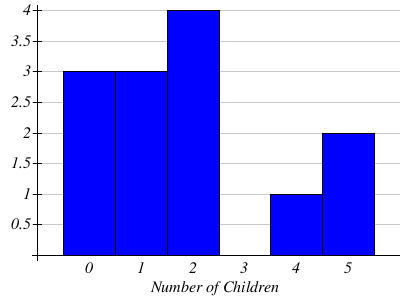
\includegraphics[width=\linewidth]{generated/problems/images/mom-6749-1.png}
\end{image}%
How many adults were questioned?%
\par
\fillintext{20}%
\par
What percentage of the adults questioned had 2 children?%
\par
\fillintext{20} \%%
\par\smallskip%
\noindent\textbf{\blocktitlefont Answer}.\hypertarget{handout-Data-5-1-2}{}\quad{}%
\begin{itemize}[label=\ptxlistdisc]
\item{}13%
\item{}30.769230769231%
\end{itemize}
%
\end{divisionexercise}%
\clearpage
\begin{divisionexercise}{4}{}{}{handout-Data-6-1}%
\begin{image}{0.25}{0.5}{0.25}{-1.5\baselineskip}%

\includegraphics[width=\linewidth]{generated/problems/images/mom-6996-1.png}
\end{image}%
Based on the histogram above, what is the frequency of the class containing the value 18%
\par
\fillintext{20}%
\par\smallskip%
\noindent\textbf{\blocktitlefont Answer}.\hypertarget{handout-Data-6-1-2}{}\quad{}%
\begin{itemize}[label=\ptxlistdisc]
\item{}6%
\end{itemize}
%
\end{divisionexercise}%
\clearpage
\begin{divisionexercise}{5}{}{}{handout-Data-7-1}%
The line graph below shows the number of times Maria drove her car each day of the week.%
\begin{image}{0.335}{0.33}{0.335}{}%

\includegraphics[width=\linewidth]{generated/problems/images/mom-1051-1.png}
\end{image}%
How many times did Maria drive her car on day 4?%
\par
\fillintext{20}%
\par\smallskip%
\noindent\textbf{\blocktitlefont Answer}.\hypertarget{handout-Data-7-1-2}{}\quad{}%
\begin{itemize}[label=\ptxlistdisc]
\item{}4%
\end{itemize}
%
\end{divisionexercise}%
\clearpage
\begin{divisionexercise}{6}{}{}{handout-Data-8-1}%
Kara categorized her spending for this month into four categories: Rent, Food, Fun, and Other.  The amounts she spent in each category are pictured here.%
\begin{image}{0.335}{0.33}{0.335}{}%

\includegraphics[width=\linewidth]{generated/problems/images/mom-1054-1.png}
\end{image}%
What percent of her total spending did she spend on Food?  Answer to the nearest whole percent.%
\par
\fillintext{20} \%%
\par\smallskip%
\noindent\textbf{\blocktitlefont Answer}.\hypertarget{handout-Data-8-1-2}{}\quad{}%
\begin{itemize}[label=\ptxlistdisc]
\item{}22%
\end{itemize}
%
\end{divisionexercise}%
\end{worksheet-section}
\restoregeometry
%
%
\typeout{************************************************}
\typeout{Worksheet  15. Activity Mean, Median, Mode and Standard Deviation}
\typeout{************************************************}
%
\newgeometry{left=0.75in, right=0.75in, top=0.75in, bottom=0.75in}
\begin{worksheet-section}{Worksheet}{15. Activity Mean, Median, Mode and Standard Deviation}{}{15. Activity Mean, Median, Mode and Standard Deviation}{}{}{handout-Mean-Median-Mode-SDeviation}
Mastering data distributions is key to analyzing statistics effectively. By utilizing measures of center and spread, you can instantly summarize and compare different datasets.%
\par
\terminology{Measures of Center} help identify a typical value within a dataset.%
%
\begin{enumerate}[label={(\alph*)}]
\item{}\lititle{The Mean.}\par%
The mathematical average and central balance point of a dataset. It is calculated by dividing the sum of all values by the total count of observations.%
\item{}\lititle{The Median.}\par%
The exact middle value in an ordered dataset. If the dataset contains an even number of values, the median is computed as the average of the two central numbers.%
\item{}\lititle{The Mode.}\par%
The value that appears most frequently in a dataset. Depending on the data, a set can be bimodal (two modes), multimodal (multiple modes), or have no mode at all.%
\end{enumerate}
\begin{divisionexercise}{1}{}{}{handout-Mean-Median-Mode-SDeviation-2-4}%
The highway mileage (mpg) for a sample of 8 different models of a car company can be found below. Find the mean, median, and mode. Round to one decimal place as needed.%
\par
20, 23, 26, 28, 30, 32, 33, 33%
\par
Mean = \fillintext{20}%
\par
Median = \fillintext{20}%
\par
Mode = \fillintext{20}%
\par\smallskip%
\noindent\textbf{\blocktitlefont Answer}.\hypertarget{handout-Mean-Median-Mode-SDeviation-2-4-2}{}\quad{}%
\begin{itemize}[label=\ptxlistdisc]
\item{}28.1%
\item{}29%
\item{}33%
\item{}%
\end{itemize}
%
\end{divisionexercise}%
\clearpage
\begin{divisionexercise}{2}{}{}{handout-Mean-Median-Mode-SDeviation-3-1}%
\begin{center}%
{\tabularfont%
\begin{tabular}{l}
Mini-Lesson: Mean, Median, and Mode\tabularnewline[0pt]
\emph{Work through the Lesson and record your work neatly in the Notebook.  When you are finished, click the check box below and then click submit (Required).}\tabularnewline[0pt]
\tabularnewline[0pt]
\multicolumn{1}{m{0.2\linewidth}}{\raggedright%
%
\begin{enumerate}[label={(\alph*)}]
\item{}I have completed this section of the Mini-Lesson and am ready to continue.%
\end{enumerate}
%
}
\end{tabular}
}%
\end{center}%
\par\smallskip%
\noindent\textbf{\blocktitlefont Answer}.\hypertarget{handout-Mean-Median-Mode-SDeviation-3-1-2}{}\quad{}%
\begin{itemize}[label=\ptxlistdisc]
\item{}I have completed this section of the Mini-Lesson and am ready to continue.%
\end{itemize}
%
\end{divisionexercise}%
\begin{divisionexercise}{3}{}{}{handout-Mean-Median-Mode-SDeviation-3-2}%
If you have the following test scores:  \(\displaystyle{72}\), \(\displaystyle{66}\), \(\displaystyle{84}\), \(\displaystyle{72}\), \(\displaystyle{60}\), and \(\displaystyle{72}\), what is your mean test score?%
\par
\fillintext{20}%
\par\smallskip%
\noindent\textbf{\blocktitlefont Answer}.\hypertarget{handout-Mean-Median-Mode-SDeviation-3-2-2}{}\quad{}%
\begin{itemize}[label=\ptxlistdisc]
\item{}71%
\end{itemize}
%
\end{divisionexercise}%
\clearpage
Moving beyond the range, the second primary measure of variation is the \terminology{standard deviation}. While the range is calculated from only two values, the standard deviation depends on every single data point within the dataset. Essentially, it summarizes how far each individual score typically deviates from the mathematical mean.%
\par
When comparing datasets, the standard deviation provides valuable insight into consistency:%
\begin{listptx}{List}{\textbf{}}{handout-Mean-Median-Mode-SDeviation-4-3}{}%
A \terminology{smaller standard deviation} indicates that the data values are highly concentrated around the center.%
A \terminology{larger standard deviation} signals that the data points are highly dispersed and variable.%
\end{listptx}%
\begin{divisionexercise}{4}{}{}{handout-Mean-Median-Mode-SDeviation-4-4}%
\begin{center}%
{\tabularfont%
\begin{tabular}{l}
Which of the following does NOT reveal the variation (spread) of the data?  \emph{Check all that apply.}\tabularnewline[0pt]
\multicolumn{1}{m{0.2\linewidth}}{\raggedright%
%
\begin{enumerate}[label={(\alph*)}]
\item{}Standard Deviation%
\item{}Mean%
\item{}Range%
\item{}Median%
\item{}Mode%
\end{enumerate}
%
}
\end{tabular}
}%
\end{center}%
\par\smallskip%
\noindent\textbf{\blocktitlefont Answer}.\hypertarget{handout-Mean-Median-Mode-SDeviation-4-4-2}{}\quad{}%
\begin{itemize}[label=\ptxlistdisc]
\item{}Mean%
\par
Mode%
\par
Median%
\end{itemize}
%
\end{divisionexercise}%
\clearpage
\begin{divisionexercise}{5}{}{}{handout-Mean-Median-Mode-SDeviation-5-1}%
Two classes were given identical quizzes.%
\par
Class A had a mean score of 8.7 and a standard deviation of 1%
\par
Class B had a mean score of 7.7 and a standard deviation of 0.8%
\par
Which class scored better on average?%
\par
%
\begin{enumerate}[label={(\alph*)}]
\item{}Class A%
\item{}Class B%
\end{enumerate}
%
\par
Which class had more consistent scores?%
\par
%
\begin{enumerate}[label={(\alph*)}]
\item{}Class A%
\item{}Class B%
\end{enumerate}
%
\par\smallskip%
\noindent\textbf{\blocktitlefont Answer}.\hypertarget{handout-Mean-Median-Mode-SDeviation-5-1-2}{}\quad{}%
\begin{itemize}[label=\ptxlistdisc]
\item{}A: Class A%
\item{}B: Class B%
\end{itemize}
%
\end{divisionexercise}%
\clearpage
\begin{divisionexercise}{6}{}{}{handout-Mean-Median-Mode-SDeviation-6-1}%
Part 1 of 2%
\par
a) Suppose Precious makes an 82 on the next quiz. Would the standard deviation of her 12 quiz scores be greater than, equal to, or less than 3? Justify your answer.%
\par
The standard deviation will be%
\par
%
\begin{enumerate}[label={(\alph*)}]
\item{}greater than%
\item{}less than%
\item{}equal to%
\end{enumerate}
%
\par
The quiz score of 82 is%
\par
%
\begin{enumerate}[label={(\alph*)}]
\item{}equal to%
\item{}less than%
\item{}greater than%
\end{enumerate}
%
\par
%
\begin{enumerate}[label={(\alph*)}]
\item{}0%
\item{}1%
\item{}3%
\end{enumerate}
%
\par
This will%
\par
%
\begin{enumerate}[label={(\alph*)}]
\item{}increase%
\item{}not effect%
\item{}decrease%
\end{enumerate}
%
\par
Part 2 of 2%
\par
The standard deviation will be%
\par
%
\begin{enumerate}[label={(\alph*)}]
\item{}greater than%
\item{}less than%
\item{}equal to%
\end{enumerate}
%
\par
The quiz score of 23 is%
\par
%
\begin{enumerate}[label={(\alph*)}]
\item{}equal to%
\item{}very close to%
\item{}very far from%
\end{enumerate}
%
\par
%
\begin{enumerate}[label={(\alph*)}]
\item{}much more than 3%
\item{}much less than 3%
\end{enumerate}
%
\par
This will%
\par
%
\begin{enumerate}[label={(\alph*)}]
\item{}increase%
\item{}decrease%
\item{}not effect%
\end{enumerate}
%
\par\smallskip%
\noindent\textbf{\blocktitlefont Answer}.\hypertarget{handout-Mean-Median-Mode-SDeviation-6-1-2}{}\quad{}%
\begin{itemize}[label=\ptxlistdisc]
\item{}B: less than%
\item{}A: equal to%
\item{}A: 0%
\item{}C: decrease%
\item{}A: greater than%
\item{}C: very far from%
\item{}A: much more than 3%
\item{}A: increase%
\end{itemize}
%
\end{divisionexercise}%
\end{worksheet-section}
\restoregeometry
%
%
\typeout{************************************************}
\typeout{Worksheet  16. Activity The Empirical rule and z-scores}
\typeout{************************************************}
%
\newgeometry{left=0.75in, right=0.75in, top=0.75in, bottom=0.75in}
\begin{worksheet-section}{Worksheet}{16. Activity The Empirical rule and z-scores}{}{16. Activity The Empirical rule and z-scores}{}{}{handout-Empirical-zscore}
In data analysis, we evaluate how extreme a specific data point is by calculating exactly how many standard deviations it sits away from the center (mean).%
%
\begin{enumerate}[label={(\alph*)}]
\item{}\terminology{The Normal Distribution} A normal distribution is a perfectly symmetrical, bell-shaped curve where data points cluster predictably around the center:%
%
\begin{itemize}[label=\ptxlistdisc]
\item{}Below Mean: Exactly 50\% of the data lies below the mean.%
\item{}Above Mean: Exactly 50\% of the data lies above the mean.%
\end{itemize}
\item{}\terminology{The Empirical Rule (68-95-99.7 Rule)} For normally distributed data, almost all observations fall within three standard deviations of the mean:%
%
\begin{itemize}[label=\ptxlistdisc]
\item{}68\% of data points fall within 1 standard deviation.%
\item{}95\% of data points fall within 2 standard deviations.%
\item{}99.7\% of data points fall within 3 standard deviations.%
\end{itemize}
\end{enumerate}
\begin{divisionexercise}{1}{}{}{handout-Empirical-zscore-2-3}%
In a mid-size company, the distribution of the number of phone calls answered each day by each of the 12 receptionists is bell-shaped and has a mean of 41 and a standard deviation of 10. Using the empirical rule (as presented in the book), what is the approximate percentage of daily phone calls numbering between 31 and 51?%
\par
Do not enter the percent symbol.%
\par
ans = \fillintext{20} \%%
\par\smallskip%
\noindent\textbf{\blocktitlefont Answer}.\hypertarget{handout-Empirical-zscore-2-3-2}{}\quad{}%
\begin{itemize}[label=\ptxlistdisc]
\item{}68%
\end{itemize}
%
\end{divisionexercise}%
\clearpage
\begin{divisionexercise}{2}{}{}{handout-Empirical-zscore-3-1}%
The maintenance department at the main campus of a large state university receives daily requests to replace fluorecent lightbulbs. The distribution of the number of daily requests is bell-shaped and has a mean of 43 and a standard deviation of 8.%
\par
Using the 68-95-99.7 rule, what is the approximate percentage of lightbulb replacement requests numbering between 27 and 43?%
\par
Answer = \fillintext{20} \%%
\par
\emph{(Type answer as a percent, do not enter the percent symbol)}%
\par
Below is the GeoGebra Empirical Rule Calculator. If this app is too small to view, you can open the application here in a new window.%
\par\smallskip%
\noindent\textbf{\blocktitlefont Answer}.\hypertarget{handout-Empirical-zscore-3-1-2}{}\quad{}%
\begin{itemize}[label=\ptxlistdisc]
\item{}47.5%
\end{itemize}
%
\end{divisionexercise}%
\clearpage
\begin{divisionexercise}{3}{}{}{handout-Empirical-zscore-4-1}%
Empirical Rule Problem%
\par
In geology, the density of granite is known to follow a normal distribution with a mean of 2.5 g\slash{}cm³ and a standard deviation of 0.025 g\slash{}cm³.%
\par
%
\begin{itemize}[label=\ptxlistdisc]
\item{}Using the \href{https://www.geogebra.org/m/xttfsxzr}{Empirical Rule Calculator}, determine the percentage of granite samples that have a density between 2.425 g\slash{}cm³ and 2.55 g\slash{}cm³.%
\par
\fillintext{5} \%%
\par
(Round to 2 decimal places.)%
\item{}Using the \href{https://www.geogebra.org/m/xttfsxzr}{Empirical Rule Calculator}, determine the percentage of granite samples that have a density less than 2.575 g\slash{}cm³%
\par
\fillintext{5} \%%
\par
(Round to 2 decimal places.)%
\item{}Using the \href{https://www.geogebra.org/m/xttfsxzr}{Empirical Rule Calculator}, determine the percentage of granite samples that have a density greater than 2.45 g\slash{}cm³%
\par
\fillintext{5} \%%
\par
(Round to 2 decimal places.)%
\end{itemize}
%
\par\smallskip%
\noindent\textbf{\blocktitlefont Answer}.\hypertarget{handout-Empirical-zscore-4-1-2}{}\quad{}%
\begin{itemize}[label=\ptxlistdisc]
\item{}97.35%
\item{}99.85%
\item{}97.5%
\end{itemize}
%
\end{divisionexercise}%
\clearpage
A z-score measures exactly how many standard deviations a specific data value lies above or below the mean, offering an exact way to evaluate how extreme a value is within a dataset. While the Empirical Rule provides quick approximations for data falling exactly one, two, or three standard deviations from the center, z-scores provide unlimited precision for values that fall anywhere in between these integers. By connecting these standardized values to probability density distributions, you can calculate the exact probability of a data point falling between two specified scores, or work backward to find a target z-score given a specific probability threshold.%
\par
To find this standardized value, use the z-score formula:%
\begin{equation*}
z = \frac{x - \text{mean}}{\text{standard deviation}}\text{.}
\end{equation*}
For example, with mean = 65 and standard deviation = 3, a score of 59 gives:%
\begin{equation*}
z = \frac{59 - 65}{3} = -2\text{.}
\end{equation*}
This means the value is 2 standard deviations below the mean.%
\clearpage
\begin{divisionexercise}{4}{}{}{handout-Empirical-zscore-6-1}%
Suppose that the scores on a statewide standardized test are normally distributed with a mean of 77 and a standard deviation of 4.  Estimate the percentage of scores that were%
\par
(a) between 69 and 85.%
\par
\fillintext{2} \%%
\par
(b) above 81.%
\par
\fillintext{2} \%%
\par
(c) below 69.%
\par
\fillintext{2} \%%
\par
(d) between 69 and 89.%
\par
\fillintext{2} \%%
\par\smallskip%
\noindent\textbf{\blocktitlefont Answer}.\hypertarget{handout-Empirical-zscore-6-1-2}{}\quad{}%
\begin{itemize}[label=\ptxlistdisc]
\item{}95%
\item{}16%
\item{}2.5%
\item{}97.35%
\end{itemize}
%
\end{divisionexercise}%
\clearpage
\begin{divisionexercise}{5}{}{}{handout-Empirical-zscore-7-1}%
The graph of a normal curve with labels is shown below. Use it to answer the questions below.%
\begin{image}{0.085}{0.83}{0.085}{}%

\includegraphics[width=\linewidth]{generated/problems/images/mom-450663-1.png}
\end{image}%
(a)  What is the mean?%
\par
\(\displaystyle\mu=\)\fillintext{5}%
\par
(b) What is the standard deviation?%
\par
\(\displaystyle\sigma=\)\fillintext{5}%
\par
(c) What percent of the values of \(\displaystyle{X}\) should fall between 46 and 49?%
\par
\fillintext{5}\%%
\par
(d) Which value of \(\displaystyle{X}\) corresponds to a \(\displaystyle{z}\)-score of \(\displaystyle-{2}\) ?%
\par
\fillintext{5}%
\par\smallskip%
\noindent\textbf{\blocktitlefont Answer}.\hypertarget{handout-Empirical-zscore-7-1-2}{}\quad{}%
\begin{itemize}[label=\ptxlistdisc]
\item{}46%
\item{}3%
\item{}34%
\item{}40%
\end{itemize}
%
\end{divisionexercise}%
\end{worksheet-section}
\restoregeometry
%
%
\typeout{************************************************}
\typeout{Worksheet  17. Scatter plots and Regrssion lines}
\typeout{************************************************}
%
\newgeometry{left=0.75in, right=0.75in, top=0.75in, bottom=0.75in}
\begin{worksheet-section}{Worksheet}{17. Scatter plots and Regrssion lines}{}{17. Scatter plots and Regrssion lines}{}{}{handout-Regression}
When two numerical variables are collected for every person or object in a sample, their relationship can be visually displayed using a \terminology{scatter plot}. In a scatter plot, each point represents a single observation, with its horizontal and vertical positions determined by the values of the two variables. This visual layout allows researchers to determine whether the two quantities are related; if a clear pattern emerges, the variables are said to be \terminology{correlated.}%
\par
However, it is critical to remember that correlation does not imply causation. For instance, while a scatter plot might reveal a strong negative correlation between education levels and prejudice, we cannot conclude that increasing education directly causes a person's level of prejudice to decrease.%
\clearpage
\begin{divisionexercise}{1}{}{}{handout-Regression-3-1}%
Creating and Analyzing Scatter Plots%
\par
\emph{Create Scatterplots for each of the tables of data below using your graphing calculator.  Determine which of the graphs most closely matches each table.  Then decide which table is Least Linear, Moderately Linear and Most Linear}%
\par
Table 1 - Matching Options: (a) B, (b) A, (c) C \textbar{} Behavior Options: (a) Least Linear, (b) Moderately Linear, (c) Most Linear \textbar{} Data: (500, 8069), (520, 8221), (540, 8796), (560, 8894), (580, 9349), (600, 9669) \textbar{} Graph: A) \begin{image}{0.4}{0.2}{0.4}{}%
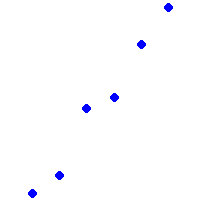
\includegraphics[width=\linewidth]{generated/problems/images/mom-23927-1.png}
\end{image}%
%
\par
Table 2 - Matching Options: (a) C, (b) B, (c) A \textbar{} Behavior Options: (a) Moderately Linear, (b) Most Linear, (c) Least Linear \textbar{} Data: (500, 101), (520, 197), (540, 357), (560, 581), (580, 739), (600, 1221) \textbar{} Graph: B) \begin{image}{0.4}{0.2}{0.4}{}%
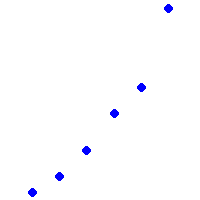
\includegraphics[width=\linewidth]{generated/problems/images/mom-23927-2.png}
\end{image}%
%
\par
Table 3 - Matching Options: (a) B, (b) A, (c) C \textbar{} Behavior Options: (a) Moderately Linear, (b) Most Linear, (c) Least Linear \textbar{} Data: (500, 4069), (520, 2749), (540, 5486), (560, 3184), (580, 4709), (600, 4869) \textbar{} Graph: C) \begin{image}{0.4}{0.2}{0.4}{}%
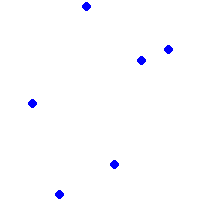
\includegraphics[width=\linewidth]{generated/problems/images/mom-23927-3.png}
\end{image}%
%
\par\smallskip%
\noindent\textbf{\blocktitlefont Answer}.\hypertarget{handout-Regression-3-1-2}{}\quad{}%
\begin{itemize}[label=\ptxlistdisc]
\item{}B: A%
\item{}C: Most Linear%
\item{}B: B%
\item{}A: Moderately Linear%
\item{}C: C%
\item{}C: Least Linear%
\end{itemize}
%
\end{divisionexercise}%
\clearpage
\begin{divisionexercise}{2}{}{}{handout-Regression-4-1}%
Here is a scatter plot for a set of bivariate data.%
\begin{image}{0.335}{0.33}{0.335}{}%

\includegraphics[width=\linewidth]{generated/problems/images/mom-337072-1.png}
\end{image}%
Is the Pearson correlation coefficient an appropriate measure of the strength of a linear relationship for this data set? yes%
\par
no%
\par\smallskip%
\noindent\textbf{\blocktitlefont Answer}.\hypertarget{handout-Regression-4-1-2}{}\quad{}%
\begin{itemize}[label=\ptxlistdisc]
\item{}A: yes%
\end{itemize}
%
\end{divisionexercise}%
\clearpage
Simple \terminology{linear regression} is a statistical method used to model the relationship between a single independent variable and a continuous dependent variable. By fitting a straight line of best fit to the observed data, this technique allows you to visualize and predict trends.%
\par
The equation of this regression line is typically expressed as a linear function in the form \(y = mx + b\), where \(m\) represents the slope of the line and \(b\) represents the y-intercept.%
\begin{divisionexercise}{3}{}{}{handout-Regression-5-3}%
\begin{center}%
{\tabularfont%
\begin{tabular}{l}
Linear Functions and Applications\tabularnewline[0pt]
\emph{Which of the following statements are true when creating an approximate linear model for a given data set?  Check all that apply.}\tabularnewline[0pt]
\multicolumn{1}{m{0.2\linewidth}}{\raggedright%
%
\begin{enumerate}[label={(\alph*)}]
\item{}It provides a way to make predictions on data points outside the given data set%
\item{}It is called Linear Regression%
\item{}It is called Finding the Line of Best Fit%
\item{}It can only be done if the data is perfectly linear.%
\end{enumerate}
%
}
\end{tabular}
}%
\end{center}%
\par\smallskip%
\noindent\textbf{\blocktitlefont Answer}.\hypertarget{handout-Regression-5-3-2}{}\quad{}%
\begin{itemize}[label=\ptxlistdisc]
\item{}It is called Linear Regression%
\par
It is called Finding the Line of Best Fit%
\par
It provides a way to make predictions on data points outside the given data set%
\end{itemize}
%
\end{divisionexercise}%
\clearpage
\begin{divisionexercise}{4}{}{}{handout-Regression-6-1}%
Analyze the residuals of a linear regression model and select the best response.%
\par
\emph{Criteria is simple evaluation of possible indications of an exponential model vs. linear model)}%
\par
\emph{Note: this question will not generate a new version of the question or graph.}%
\begin{image}{0.14}{0.72}{0.14}{}%
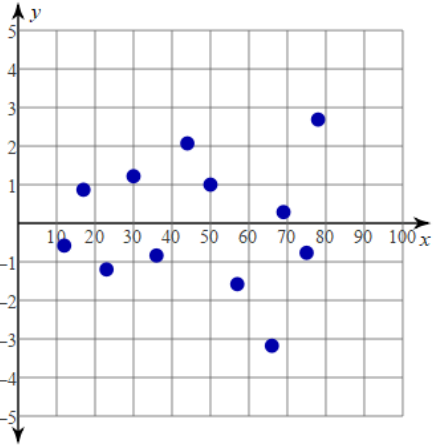
\includegraphics[width=\linewidth]{generated/problems/images/mom-904695-1.PNG}
\end{image}%
%
\begin{enumerate}[label={(\alph*)}]
\item{}no, the residual plot does not show a curve%
\item{}yes, the residual plot shows a curve%
\item{}no, the residual plot shows a curve%
\item{}yes, the residual plot does not show a curve%
\end{enumerate}
%
\par\smallskip%
\noindent\textbf{\blocktitlefont Answer}.\hypertarget{handout-Regression-6-1-2}{}\quad{}%
\begin{itemize}[label=\ptxlistdisc]
\item{}D: yes, the residual plot does not show a curve%
\end{itemize}
%
\end{divisionexercise}%
\end{worksheet-section}
\restoregeometry
\end{chapterptx}
%
%
\typeout{************************************************}
\typeout{Chapter 6 Practical Application \& Hands-On Sessions}
\typeout{************************************************}
%
\begin{chapterptx}{Chapter}{Practical Application \& Hands-On Sessions}{}{Practical Application \& Hands-On Sessions}{}{}{Hands-On-Sessions}
\renewcommand*{\chaptername}{Chapter}
\begin{introduction}{}%
These notes are intended strictly for a quick review of each chapter. They do not substitute for attending lectures or reading the assigned textbook.%
\end{introduction}%
%
%
\typeout{************************************************}
\typeout{Worksheet  1. Voting Methods Handout}
\typeout{************************************************}
%
\newgeometry{left=0.75in, right=0.75in, top=0.75in, bottom=0.75in}
\begin{worksheet-section}{Worksheet}{1. Voting Methods Handout}{}{1. Voting Methods Handout}{}{}{handout-voting-methods}
This handout outlines the core procedural rules, calculation steps, and the four primary preference-ballot voting methods:%
\begin{introduction}{}%
%
\begin{itemize}[label=\ptxlistdisc]
\item{}\lititle{The Plurality Method.}\par%
 Selecting the candidate who receives the most first-place votes, regardless of whether they achieve a strict majority.%
\item{}\lititle{The Plurality-with-Elimination Method.}\par%
 An iterative process where the candidate with the fewest first-place votes is eliminated, and their ballots are redistributed, continuing until a candidate achieves a true majority.%
\item{}\lititle{The Borda Count Method.}\par%
 A point-based system where points are assigned to each ranking position on a ballot, and the candidate with the highest total points across all ballots wins.%
\item{}\lititle{The Pairwise Comparison Method.}\par%
 A head-to-head match-up approach where every candidate is compared one-on-one against every other candidate to see who wins the most direct duels, identifying a Condorcet candidate if one exists.%
\end{itemize}
%
\end{introduction}%
Exercises and Workspaces%
\begin{divisionexercise}{1}{}{1.5in}{ws-ex-plurality}%
Four students are running for president of their residence hall: Debra (D), Farah (F), Jorge (J), and Hillary (H). The votes of their fellow students are summarized in the following preferences table. Who is declared the president using the \terminology{plurality} method?%
\begin{center}%
{\tabularfont%
\begin{tabular}{AlAlAlAlAlAlA}\hrulethin
{\bfseries{}Number of Votes}&\multicolumn{1}{cA}{{\bfseries{}52}}&\multicolumn{1}{cA}{{\bfseries{}45}}&\multicolumn{1}{cA}{{\bfseries{}13}}&\multicolumn{1}{cA}{{\bfseries{}9}}&\multicolumn{1}{cA}{{\bfseries{}4}}\tabularnewline\hrulethin
First choice&\multicolumn{1}{cA}{D}&\multicolumn{1}{cA}{F}&\multicolumn{1}{cA}{J}&\multicolumn{1}{cA}{F}&\multicolumn{1}{cA}{H}\tabularnewline\hrulethin
Second choice&\multicolumn{1}{cA}{F}&\multicolumn{1}{cA}{J}&\multicolumn{1}{cA}{F}&\multicolumn{1}{cA}{J}&\multicolumn{1}{cA}{J}\tabularnewline\hrulethin
Third choice&\multicolumn{1}{cA}{H}&\multicolumn{1}{cA}{H}&\multicolumn{1}{cA}{H}&\multicolumn{1}{cA}{D}&\multicolumn{1}{cA}{D}\tabularnewline\hrulethin
Fourth choice&\multicolumn{1}{cA}{J}&\multicolumn{1}{cA}{D}&\multicolumn{1}{cA}{D}&\multicolumn{1}{cA}{H}&\multicolumn{1}{cA}{F}\tabularnewline\hrulethin
\end{tabular}
}%
\end{center}%
\par\smallskip%
\noindent\textbf{\blocktitlefont Solution}.\hypertarget{ws-ex-plurality-2}{}\quad{}First-choice totals are D = 52, F = 54, J = 13, and H = 4. The winner by the plurality method is \terminology{F}.%
\end{divisionexercise}%
\clearpage
\begin{divisionexercise}{2}{}{2.5in}{ws-ex-elimination}%
Four students are running for president of their residence hall: Debra (D), Farah (F), Jorge (J), and Hillary (H). The votes of their fellow students are summarized in the following preferences table. Who is declared the president using the \terminology{plurality-with-elimination} method?%
\begin{center}%
{\tabularfont%
\begin{tabular}{AlAlAlAlAlAlA}\hrulethin
{\bfseries{}Number of Votes}&\multicolumn{1}{cA}{{\bfseries{}52}}&\multicolumn{1}{cA}{{\bfseries{}45}}&\multicolumn{1}{cA}{{\bfseries{}13}}&\multicolumn{1}{cA}{{\bfseries{}9}}&\multicolumn{1}{cA}{{\bfseries{}4}}\tabularnewline\hrulethin
First choice&\multicolumn{1}{cA}{D}&\multicolumn{1}{cA}{F}&\multicolumn{1}{cA}{J}&\multicolumn{1}{cA}{F}&\multicolumn{1}{cA}{H}\tabularnewline\hrulethin
Second choice&\multicolumn{1}{cA}{F}&\multicolumn{1}{cA}{J}&\multicolumn{1}{cA}{F}&\multicolumn{1}{cA}{J}&\multicolumn{1}{cA}{J}\tabularnewline\hrulethin
Third choice&\multicolumn{1}{cA}{H}&\multicolumn{1}{cA}{H}&\multicolumn{1}{cA}{H}&\multicolumn{1}{cA}{D}&\multicolumn{1}{cA}{D}\tabularnewline\hrulethin
Fourth choice&\multicolumn{1}{cA}{J}&\multicolumn{1}{cA}{D}&\multicolumn{1}{cA}{D}&\multicolumn{1}{cA}{H}&\multicolumn{1}{cA}{F}\tabularnewline\hrulethin
\end{tabular}
}%
\end{center}%
\par\smallskip%
\noindent\textbf{\blocktitlefont Solution}.\hypertarget{ws-ex-elimination-2}{}\quad{}Eliminate H first (4 votes), which transfers to J, giving J 17 votes. Then eliminate J; all 17 J ballots transfer to F. Final totals are D = 52 and F = 71, so the plurality-with-elimination winner is \terminology{F}.%
\end{divisionexercise}%
\clearpage
\begin{divisionexercise}{3}{}{2.5in}{ws-ex-borda}%
Four students are running for president of their residence hall: Debra (D), Farah (F), Jorge (J), and Hillary (H). The votes of their fellow students are summarized in the following preferences table. Who is declared the president using the \terminology{Borda count} method?%
\begin{center}%
{\tabularfont%
\begin{tabular}{AlAlAlAlAlAlA}\hrulethin
{\bfseries{}Number of Votes}&\multicolumn{1}{cA}{{\bfseries{}52}}&\multicolumn{1}{cA}{{\bfseries{}45}}&\multicolumn{1}{cA}{{\bfseries{}13}}&\multicolumn{1}{cA}{{\bfseries{}9}}&\multicolumn{1}{cA}{{\bfseries{}4}}\tabularnewline\hrulethin
First choice&\multicolumn{1}{cA}{D}&\multicolumn{1}{cA}{F}&\multicolumn{1}{cA}{J}&\multicolumn{1}{cA}{F}&\multicolumn{1}{cA}{H}\tabularnewline\hrulethin
Second choice&\multicolumn{1}{cA}{F}&\multicolumn{1}{cA}{J}&\multicolumn{1}{cA}{F}&\multicolumn{1}{cA}{J}&\multicolumn{1}{cA}{J}\tabularnewline\hrulethin
Third choice&\multicolumn{1}{cA}{H}&\multicolumn{1}{cA}{H}&\multicolumn{1}{cA}{H}&\multicolumn{1}{cA}{D}&\multicolumn{1}{cA}{D}\tabularnewline\hrulethin
Fourth choice&\multicolumn{1}{cA}{J}&\multicolumn{1}{cA}{D}&\multicolumn{1}{cA}{D}&\multicolumn{1}{cA}{H}&\multicolumn{1}{cA}{F}\tabularnewline\hrulethin
\end{tabular}
}%
\end{center}%
\par\smallskip%
\noindent\textbf{\blocktitlefont Solution}.\hypertarget{ws-ex-borda-2}{}\quad{}Using Borda scores 3-2-1-0, the totals are D = 169, F = 292, J = 155, and H = 122. The Borda count winner is \terminology{F}.%
\end{divisionexercise}%
\clearpage
\begin{divisionexercise}{4}{}{2.5in}{ws-ex-pairwise}%
Four students are running for president of their residence hall: Debra (D), Farah (F), Jorge (J), and Hillary (H). The votes of their fellow students are summarized in the following preferences table. Who is declared the president using the \terminology{pairwise comparison} method? Is there a \terminology{Condorcet} winner?%
\begin{center}%
{\tabularfont%
\begin{tabular}{AlAlAlAlAlAlA}\hrulethin
{\bfseries{}Number of Votes}&\multicolumn{1}{cA}{{\bfseries{}52}}&\multicolumn{1}{cA}{{\bfseries{}45}}&\multicolumn{1}{cA}{{\bfseries{}13}}&\multicolumn{1}{cA}{{\bfseries{}9}}&\multicolumn{1}{cA}{{\bfseries{}4}}\tabularnewline\hrulethin
First choice&\multicolumn{1}{cA}{D}&\multicolumn{1}{cA}{F}&\multicolumn{1}{cA}{J}&\multicolumn{1}{cA}{F}&\multicolumn{1}{cA}{H}\tabularnewline\hrulethin
Second choice&\multicolumn{1}{cA}{F}&\multicolumn{1}{cA}{J}&\multicolumn{1}{cA}{F}&\multicolumn{1}{cA}{J}&\multicolumn{1}{cA}{J}\tabularnewline\hrulethin
Third choice&\multicolumn{1}{cA}{H}&\multicolumn{1}{cA}{H}&\multicolumn{1}{cA}{H}&\multicolumn{1}{cA}{D}&\multicolumn{1}{cA}{D}\tabularnewline\hrulethin
Fourth choice&\multicolumn{1}{cA}{J}&\multicolumn{1}{cA}{D}&\multicolumn{1}{cA}{D}&\multicolumn{1}{cA}{H}&\multicolumn{1}{cA}{F}\tabularnewline\hrulethin
\end{tabular}
}%
\end{center}%
\par\smallskip%
\noindent\textbf{\blocktitlefont Solution}.\hypertarget{ws-ex-pairwise-2}{}\quad{}In head-to-head matchups, F beats D, F beats J, and F beats H. Candidate \terminology{F} wins every pairwise comparison and is the Condorcet winner.%
\end{divisionexercise}%
\clearpage
\begin{divisionexercise}{5}{}{6.0in}{ws-ex-professors-election}%
Four professors are running for president of the League of Innovation: Doug (D), Francis (F), Gallagher (G), and Smith (S). The votes of the members in the League of Innovation are summarized in the preference table below.%
\begin{center}%
{\tabularfont%
\begin{tabular}{AlAlAlAlAlAlA}\hrulethin
{\bfseries{}Number of Votes}&\multicolumn{1}{cA}{{\bfseries{}30}}&\multicolumn{1}{cA}{{\bfseries{}22}}&\multicolumn{1}{cA}{{\bfseries{}18}}&\multicolumn{1}{cA}{{\bfseries{}10}}&\multicolumn{1}{cA}{{\bfseries{}2}}\tabularnewline\hrulethin
First Choice&\multicolumn{1}{cA}{F}&\multicolumn{1}{cA}{G}&\multicolumn{1}{cA}{S}&\multicolumn{1}{cA}{D}&\multicolumn{1}{cA}{G}\tabularnewline\hrulethin
Second Choice&\multicolumn{1}{cA}{D}&\multicolumn{1}{cA}{D}&\multicolumn{1}{cA}{G}&\multicolumn{1}{cA}{S}&\multicolumn{1}{cA}{S}\tabularnewline\hrulethin
Third Choice&\multicolumn{1}{cA}{G}&\multicolumn{1}{cA}{S}&\multicolumn{1}{cA}{D}&\multicolumn{1}{cA}{G}&\multicolumn{1}{cA}{D}\tabularnewline\hrulethin
Fourth Choice&\multicolumn{1}{cA}{S}&\multicolumn{1}{cA}{F}&\multicolumn{1}{cA}{F}&\multicolumn{1}{cA}{F}&\multicolumn{1}{cA}{F}\tabularnewline\hrulethin
\end{tabular}
}%
\end{center}%
%
\begin{enumerate}[label={(\alph*)}]
\item{}How many members voted in this election?%
\item{}Using the plurality method, who becomes the new president?%
\item{}Using the plurality-with-elimination method, who becomes the new president?%
\item{}Using the Borda count method, who becomes the new president?%
\item{}Using the pairwise comparison method, who becomes the new president?%
\end{enumerate}
\par\smallskip%
\noindent\textbf{\blocktitlefont Solution}.\hypertarget{ws-ex-professors-election-2}{}\quad{}Total votes = 82. Plurality totals are F = 30, G = 24, S = 18, and D = 10, so \terminology{F} wins by plurality.%
\par
For plurality-with-elimination, D is eliminated first and its 10 votes transfer to S, then G is eliminated and its votes transfer to S, giving \terminology{S} the win.%
\par
Using Borda scores 3-2-1-0, the totals are D = 154, G = 148, S = 100, and F = 90. The Borda winner is \terminology{D}.%
\par
In pairwise comparison, G beats D, G beats F, and G beats S, so the pairwise winner is \terminology{G}.%
\end{divisionexercise}%
\end{worksheet-section}
\restoregeometry
%
%
\typeout{************************************************}
\typeout{Worksheet  2. Apportionment Handout}
\typeout{************************************************}
%
\newgeometry{left=0.75in, right=0.75in, top=0.75in, bottom=0.75in}
\begin{worksheet-section}{Worksheet}{2. Apportionment Handout}{}{2. Apportionment Handout}{}{}{handout-apportionment}
\begin{introduction}{}%
This handout covers the core metrics and sequential steps for the major historic apportionment methods:%
\par
%
\begin{itemize}[label=\ptxlistdisc]
\item{}Calculating the Standard Divisor, Standard Quotas, Lower Quotas, and Upper Quotas.%
\item{}\lititle{Hamilton's Method.}\par%
 Assigning initial seats using the Lower Quota, then distributing surplus seats based on the largest fractional remainders.%
\item{}\lititle{Jefferson's Method.}\par%
 Finding a Modified Divisor that alters the quotas so that the sum of the Lower Quotas exactly matches the total seats.%
\item{}\lititle{Adams's Method.}\par%
 Finding a Modified Divisor that alters the quotas so that the sum of the Upper Quotas exactly matches the total seats.%
\end{itemize}
%
\end{introduction}%
Exercises and Workspaces%
\begin{divisionexercise}{1}{}{}{handout-apportionment-4-1}%
A hospital has a nursing staff of 250 nurses working in four shifts:%
\begin{itemize}[label=\ptxlistdisc]
\item{}\lititle{Shift A: 7:00 A.M. to 1:00 P.M..}\par%
%
\item{}\lititle{Shift B: 1:00 P.M. to 7:00 P.M..}\par%
%
\item{}\lititle{Shift C: 7:00 P.M. to 1:00 A.M..}\par%
%
\item{}\lititle{Shift D: 1:00 A.M. to 7:00 A.M..}\par%
%
\end{itemize}
The number of nurses apportioned to each shift is based on the average number of patients per shift, given in the table below. Use \alert{Hamilton's method} to apportion the 250 nurses among the shifts at the hospital.%
\begin{center}%
{\tabularfont%
\begin{tabular}{AlAcAcAcAcA}\hrulethin
{\bfseries{}Shift}&{\bfseries{}A}&{\bfseries{}B}&{\bfseries{}C}&{\bfseries{}D}\tabularnewline\hrulethin
Average Patients&453&650&547&350\tabularnewline\hrulethin
\end{tabular}
}%
\end{center}%
\par\smallskip%
\noindent\textbf{\blocktitlefont Solution}.\hypertarget{handout-apportionment-4-1-2}{}\quad{}To complete the apportionment using Hamilton's method, we follow these sequential calculation steps:%
\par
%
\begin{enumerate}[label={(\alph*)}]
\item{}Find the Total Population: Sum the average number of patients across all shifts.%
\begin{equation*}
453 + 650 + 547 + 350 = 2000 \text{ total patients}
\end{equation*}
%
\item{}Calculate the Standard Divisor (\(d\)): Divide the total population by the total number of items (250 nurses) to be allocated.%
\begin{equation*}
d = \frac{2000}{250} = 8
\end{equation*}
%
\item{}Find Standard and Lower Quotas: Divide each shift's patient count by the Standard Divisor (\(8\)). The Lower Quota is found by rounding down to the nearest whole integer.%
\begin{itemize}[label=\ptxlistdisc]
\item{}Shift A: \(\frac{453}{8} = 56.625\) (Lower Quota = 56)%
\item{}Shift B: \(\frac{650}{8} = 81.250\) (Lower Quota = 81)%
\item{}Shift C: \(\frac{547}{8} = 68.375\) (Lower Quota = 68)%
\item{}Shift D: \(\frac{350}{8} = 43.750\) (Lower Quota = 43)%
\end{itemize}
%
\item{}Distribute Surplus Items: Summing the lower quotas gives \(56 + 81 + 68 + 43 = 248\) nurses. Since we must allocate 250 nurses, there is a surplus of \(250 - 248 = 2\) nurses. Hamilton's method gives these surplus spots to the shifts with the largest fractional remainder parts:%
\begin{itemize}[label=\ptxlistdisc]
\item{}Shift D has the largest remainder (\(0.750\)) and receives \(+1\) nurse.%
\item{}Shift A has the second-largest remainder (\(0.625\)) and receives \(+1\) nurse.%
\end{itemize}
%
\end{enumerate}
%
\par
The complete apportionment layout is summarized below:%
\begin{center}%
{\tabularfont%
\begin{tabular}{AlAcAcAcAcAcA}\hrulethin
{\bfseries{}Metric \slash{} Step}&{\bfseries{}Shift A}&{\bfseries{}Shift B}&{\bfseries{}Shift C}&{\bfseries{}Shift D}&{\bfseries{}Total}\tabularnewline\hrulethin
Patients&453&650&547&350&2000\tabularnewline\hrulethin
Standard Quota&56.625&81.250&68.375&43.750&-\tabularnewline\hrulethin
Lower Quota&56&81&68&43&248\tabularnewline\hrulethin
Surplus Added&+1&0&0&+1&+2\tabularnewline\hrulethin
Final Apportionment&57&81&68&44&250\tabularnewline\hrulethin
\end{tabular}
}%
\end{center}%
\end{divisionexercise}%
\clearpage
\begin{divisionexercise}{2}{}{}{handout-apportionment-5-1}%
A hospital has a nursing staff of 250 nurses working in four shifts. The number of nurses apportioned to each shift is based on the average number of patients per shift, given in the table below. Use \alert{Jefferson's method} to apportion the 250 nurses among the shifts at the hospital.%
\begin{center}%
{\tabularfont%
\begin{tabular}{AlAcAcAcAcA}\hrulethin
{\bfseries{}Shift}&{\bfseries{}A}&{\bfseries{}B}&{\bfseries{}C}&{\bfseries{}D}\tabularnewline\hrulethin
Average Patients&453&650&547&350\tabularnewline\hrulethin
\end{tabular}
}%
\end{center}%
\par\smallskip%
\noindent\textbf{\blocktitlefont Solution}.\hypertarget{handout-apportionment-5-1-2}{}\quad{}To complete the apportionment using Jefferson's method, we apply a modified divisor so that the sum of the lower quotas exactly equals the required total.%
\par
%
\begin{enumerate}[label={(\alph*)}]
\item{}Find Total Population and Standard Divisor (\(d\)):%
\begin{equation*}
\text{Total Patients} = 453 + 650 + 547 + 350 = 2000
\end{equation*}
%
\begin{equation*}
d = \frac{2000 \text{ patients}}{250 \text{ nurses}} = 8
\end{equation*}
%
\item{}Test the Standard Divisor: Dividing each population by \(8\) and rounding down gives lower quotas of \(56, 81, 68,\) and \(43\). The sum of these initial lower quotas is \(56 + 81 + 68 + 43 = 248\). This falls short of the \(250\) nurses needed.%
\item{}Determine a Modified Divisor (\(d_m\)): Because our initial sum is too small, Jefferson's method requires us to choose a smaller divisor to increase the individual quotas. Testing a modified divisor of \(d_m = 7.93\) shifts the lower quotas upward to exactly equal \(250\).%
\end{enumerate}
%
\par
The complete apportionment computations under Jefferson's method are detailed below:%
\begin{center}%
{\tabularfont%
\begin{tabular}{AlAcAcAcAcAcA}\hrulethin
{\bfseries{}Metric \slash{} Step}&{\bfseries{}Shift A}&{\bfseries{}Shift B}&{\bfseries{}Shift C}&{\bfseries{}Shift D}&{\bfseries{}Total}\tabularnewline\hrulethin
Patients&453&650&547&350&2000\tabularnewline\hrulethin
Standard Quota (d = 8)&56.625&81.250&68.375&43.750&—\tabularnewline\hrulethin
Initial Lower Quota&56&81&68&43&248\tabularnewline\hrulethin
Modified Quota (dm = 7.93)&57.125&81.967&68.979&44.136&—\tabularnewline\hrulethin
Final Apportionment&57&81&68&44&250\tabularnewline\hrulethin
\end{tabular}
}%
\end{center}%
\end{divisionexercise}%
\clearpage
\begin{divisionexercise}{3}{}{}{handout-apportionment-6-1}%
A hospital has a nursing staff of 250 nurses working in four shifts. The number of nurses apportioned to each shift is based on the average number of patients per shift, given in the table below. Use \alert{Adams's method} to apportion the 250 nurses among the shifts at the hospital.%
\begin{center}%
{\tabularfont%
\begin{tabular}{AlAcAcAcAcA}\hrulethin
{\bfseries{}Shift}&{\bfseries{}A}&{\bfseries{}B}&{\bfseries{}C}&{\bfseries{}D}\tabularnewline\hrulethin
Average Patients&453&650&547&350\tabularnewline\hrulethin
\end{tabular}
}%
\end{center}%
\par\smallskip%
\noindent\textbf{\blocktitlefont Solution}.\hypertarget{handout-apportionment-6-1-2}{}\quad{}To complete the apportionment using Adams's method, we apply a modified divisor so that the sum of the upper quotas (rounded up) exactly equals the required total.%
\par
%
\begin{enumerate}[label={(\alph*)}]
\item{}Find Total Population and Standard Divisor (\(d\)):%
\begin{equation*}
\text{Total Patients} = 453 + 650 + 547 + 350 = 2000
\end{equation*}
%
\begin{equation*}
d = \frac{2000 \text{ patients}}{250 \text{ nurses}} = 8
\end{equation*}
%
\item{}Test the Standard Divisor: Dividing each population by \(8\) and rounding up to the next highest integer gives upper quotas of \(57, 82, 69,\) and \(44\). The sum of these initial upper quotas is \(57 + 82 + 69 + 44 = 252\). This exceeds the target of \(250\) nurses.%
\item{}Determine a Modified Divisor (\(d_m\)): Because our initial sum is too large, Adams's method requires us to choose a larger divisor to decrease the individual quotas. Testing a modified divisor of \(d_m = 8.07\) shifts the upper quotas downward to exactly equal \(250\).%
\end{enumerate}
%
\par
The complete apportionment calculations under Adams's method are organized in the accessible data layout below:%
\begin{center}%
{\tabularfont%
\begin{tabular}{AlAcAcAcAcAcA}\hrulethin
{\bfseries{}Metric \slash{} Step}&{\bfseries{}Shift A}&{\bfseries{}Shift B}&{\bfseries{}Shift C}&{\bfseries{}Shift D}&{\bfseries{}Total}\tabularnewline\hrulethin
Patients&453&650&547&350&2000\tabularnewline\hrulethin
Standard Quota (\(d=8\))&56.625&81.250&68.375&43.750&—\tabularnewline\hrulethin
Initial Upper Quota&57&82&69&44&252\tabularnewline\hrulethin
Modified Quota (\(d_m=8.07\))&56.134&80.545&67.782&43.371&—\tabularnewline\hrulethin
Final Apportionment&57&81&68&44&250\tabularnewline\hrulethin
\end{tabular}
}%
\end{center}%
\end{divisionexercise}%
\clearpage
\begin{divisionexercise}{4}{}{}{handout-apportionment-7-1}%
The police department in a large city has 180 new officers to be apportioned among 6 high-crime precincts. The total number of recorded crimes for each respective precinct is documented in the data profile below.%
 \begin{center}%
{\tabularfont%
\begin{tabular}{AlAcAcAcAcAcAcA}\hrulethin
{\bfseries{}Precinct}&{\bfseries{}A}&{\bfseries{}B}&{\bfseries{}C}&{\bfseries{}D}&{\bfseries{}E}&{\bfseries{}F}\tabularnewline\hrulethin
Crimes&446&526&835&227&338&456\tabularnewline\hrulethin
\end{tabular}
}%
\end{center}%
\begin{enumerate}[font=\bfseries,label=(\alph*),ref=\alph*]%
\item{}Use \alert{Hamilton's method} to apportion the new officers among the precincts.%
\par\smallskip%
\noindent\textbf{\blocktitlefont Solution}.\hypertarget{handout-apportionment-7-1-2-2}{}\quad{}1. Identify Metrics: Total crimes population equals \(446 + 526 + 835 + 227 + 338 + 456 = 2828\). The Standard Divisor is:%
\begin{equation*}
d = \frac{2828}{180} \approx 15.7111
\end{equation*}
%
\par
2. Distribute Remainders: Summing the lower whole quotas gives \(28 + 33 + 53 + 14 + 21 + 29 = 178\) allocations, leaving a surplus of \(2\) seats. Hamilton's method awards these seats to the largest fractional remainders: Precinct B (\(0.4795\)) and Precinct E (\(0.5134\)).%
\begin{center}%
{\tabularfont%
\begin{tabular}{AlAcAcAcAcAcAcAcA}\hrulethin
{\bfseries{}Metric \slash{} Step}&{\bfseries{}A}&{\bfseries{}B}&{\bfseries{}C}&{\bfseries{}D}&{\bfseries{}E}&{\bfseries{}F}&{\bfseries{}Total}\tabularnewline\hrulethin
Crimes&446&526&835&227&338&456&2828\tabularnewline\hrulethin
Standard Quota&28.388&33.479&53.147&14.448&21.513&29.024&—\tabularnewline\hrulethin
Lower Quota&28&33&53&14&21&29&178\tabularnewline\hrulethin
Surplus Added&0&+1&0&0&+1&0&+2\tabularnewline\hrulethin
Final Apportionment&28&34&53&14&22&29&180\tabularnewline\hrulethin
\end{tabular}
}%
\end{center}%
\par\rule{\workspacestrutwidth}{1in}%
\item{}Use \alert{Jefferson's method} to apportion the new officers among the precincts.%
\par\smallskip%
\noindent\textbf{\blocktitlefont Solution}.\hypertarget{handout-apportionment-7-1-3-2}{}\quad{}Because the initial lower quota sum (\(178\)) is too small, Jefferson's method requires modifying the divisor downward to raise the quotas. Choosing a smaller modified divisor of \(d_m = 15.46\) shifts the lower whole quotas up to hit the targeted total allocation sum of exactly \(180\).%
\begin{center}%
{\tabularfont%
\begin{tabular}{AlAcAcAcAcAcAcAcA}\hrulethin
{\bfseries{}Metric \slash{} Step}&{\bfseries{}A}&{\bfseries{}B}&{\bfseries{}C}&{\bfseries{}D}&{\bfseries{}E}&{\bfseries{}F}&{\bfseries{}Total}\tabularnewline\hrulethin
Crimes&446&526&835&227&338&456&2828\tabularnewline\hrulethin
Modified Quota&28.849&34.023&54.010&14.683&21.863&29.495&—\tabularnewline\hrulethin
Final Apportionment&28&34&54&14&21&29&180\tabularnewline\hrulethin
\end{tabular}
}%
\end{center}%
\par\rule{\workspacestrutwidth}{1in}%
\item{}Use \alert{Adams's method} to apportion the new officers among the precincts.%
\par\smallskip%
\noindent\textbf{\blocktitlefont Solution}.\hypertarget{handout-apportionment-7-1-4-2}{}\quad{}Testing the standard upper quotas (rounding fractions up) gives a sum of \(29 + 34 + 54 + 15 + 22 + 30 = 184\), which exceeds the 180 seats. Adams's method resolves this by increasing the divisor. Choosing a larger modified divisor of \(d_m = 15.94\) pushes the quotas downward so that their rounded-up total sums exactly to \(180\).%
\begin{center}%
{\tabularfont%
\begin{tabular}{AlAcAcAcAcAcAcAcA}\hrulethin
{\bfseries{}Metric \slash{} Step}&{\bfseries{}A}&{\bfseries{}B}&{\bfseries{}C}&{\bfseries{}D}&{\bfseries{}E}&{\bfseries{}F}&{\bfseries{}Total}\tabularnewline\hrulethin
Crimes&446&526&835&227&338&456&2828\tabularnewline\hrulethin
Modified Quota&27.980&32.999&52.384&14.241&21.205&28.607&—\tabularnewline\hrulethin
Final Apportionment&28&33&53&15&22&29&180\tabularnewline\hrulethin
\end{tabular}
}%
\end{center}%
\par\rule{\workspacestrutwidth}{1in}%
\end{enumerate}%
\end{divisionexercise}%
\end{worksheet-section}
\restoregeometry
%
%
\typeout{************************************************}
\typeout{Worksheet  3. Personal Finance Handout}
\typeout{************************************************}
%
\newgeometry{left=0.75in, right=0.75in, top=0.75in, bottom=0.75in}
\begin{worksheet-section}{Worksheet}{3. Personal Finance Handout}{}{3. Personal Finance Handout}{}{}{handout-finance}
\begin{introduction}{}%
This handout covers essential mathematical principles for evaluating individual savings, annuities, and debt management strategies:%
\par
%
\begin{itemize}[label=\ptxlistdisc]
\item{}\lititle{Basic Interest Calculations.}\par%
 Computing and comparing simple interest and compound interest models over various compounding periods.%
\item{}\lititle{Savings and Annuities.}\par%
 Analyzing regular deposit schedules, future value growth patterns, and long-term retirement accounts.%
\item{}\lititle{Loans and Spendings.}\par%
 Evaluating fixed-rate installment loans, calculating monthly amortization values, and managing large debts including home mortgages.%
\end{itemize}
%
\end{introduction}%
Exercises and Workspaces%
\begin{divisionexercise}{1}{}{}{handout-finance-4-1}%
In order to pay for baseball uniforms, a school takes out a \alert{simple interest} loan for \textdollar{}20,000 for 7 months at a rate of 12\%. Find the future value of the loan.%
\par\smallskip%
\noindent\textbf{\blocktitlefont Solution}.\hypertarget{handout-finance-4-1-2}{}\quad{}To find the future value of a loan using a simple interest model, we extract our known variables and evaluate using the linear simple interest equation.%
\par
Identify Given Variables:%
\begin{itemize}[label=\ptxlistdisc]
\item{}Principal (\(P\)): \(\$20,000\)%
\item{}Annual Interest Rate (\(r\)): \(12\% = 0.12\)%
\item{}Time (\(t\)): \(7 \text{ months} = \frac{7}{12} \text{ of a year}\)%
\end{itemize}
%
\par
Step-by-Step Calculation:%
\begin{enumerate}[label={(\alph*)}]
\item{}Calculate Accumulated Interest (\(I\)): Multiply Principal by Rate by Time.%
\begin{equation*}
I = P \cdot r \cdot t
\end{equation*}
%
\begin{equation*}
I = 20000 \cdot 0.12 \cdot \left(\frac{7}{12}\right)
\end{equation*}
%
\begin{equation*}
I = 20000 \cdot 0.07 = 1400
\end{equation*}
The total accumulated interest generated over the 7 months is \(\$1,400\).%
\item{}Calculate Future Value (\(A\)): Sum the initial principal amount and the newly accumulated interest.%
\begin{equation*}
A = P + I
\end{equation*}
%
\begin{equation*}
A = 20000 + 1400 = 21400
\end{equation*}
%
\end{enumerate}
%
\par
The final future value of the loan at maturity is \(\$21,400\).%
\end{divisionexercise}%
\clearpage
\begin{divisionexercise}{2}{}{}{handout-finance-5-1}%
What is the amount of the deposit needed if your financial goal is to save \textdollar{}24,000 in 3 years with a rate of 7.5\% \alert{compounded semiannually}?%
\par\smallskip%
\noindent\textbf{\blocktitlefont Solution}.\hypertarget{handout-finance-5-1-2}{}\quad{}To find the initial deposit (present value) required to meet a future financial goal with compound interest, we rearrange the compound interest formula to solve for the principal \(P\).%
\par
Identify Given Variables:%
\begin{itemize}[label=\ptxlistdisc]
\item{}Future Value Goal (\(A\)): \(\$24,000\)%
\item{}Annual Interest Rate (\(r\)): \(7.5\% = 0.075\)%
\item{}Compounding Periods per Year (\(n\)): \(2\) (semiannually)%
\item{}Time (\(t\)): \(3 \text{ years}\)%
\end{itemize}
%
\par
Step-by-Step Calculation:%
\begin{enumerate}[label={(\alph*)}]
\item{}State the Present Value Formula:%
\begin{equation*}
P = \frac{A}{\left(1 + \frac{r}{n}\right)^{nt}}
\end{equation*}
%
\item{}Substitute the Values: Find the interest rate per period (\(\frac{r}{n}\)) and total number of compounding periods (\(nt\)).%
\begin{equation*}
\frac{r}{n} = \frac{0.075}{2} = 0.0375
\end{equation*}
%
\begin{equation*}
nt = 2 \cdot 3 = 6 \text{ total compounding periods}
\end{equation*}
%
\begin{equation*}
P = \frac{24000}{(1 + 0.0375)^{6}}
\end{equation*}
%
\item{}Evaluate the Denominator:%
\begin{equation*}
P = \frac{24000}{(1.0375)^{6}}
\end{equation*}
%
\begin{equation*}
P \approx \frac{24000}{1.247179}
\end{equation*}
%
\item{}Calculate the Final Principal Amount: Divide the future goal by the compounding factor and round to the nearest cent.%
\begin{equation*}
P \approx 19243.44
\end{equation*}
%
\end{enumerate}
%
\par
The initial deposit amount needed to meet your financial goal is \(\$19,243.44\).%
\end{divisionexercise}%
\clearpage
\begin{divisionexercise}{3}{}{}{handout-finance-6-1}%
Your sister has her first child and you decide to open an annuity for your baby nephew. You deposit \textdollar{}30 \alert{at the end of each month into an annuity} that returns 2.5\% annual interest.%
\begin{enumerate}[font=\bfseries,label=(\alph*),ref=\alph*]%
\item{}How much will your nephew have in his annuity when he goes off to college (18 years from now)?%
\par\smallskip%
\noindent\textbf{\blocktitlefont Solution}.\hypertarget{handout-finance-6-1-2-2}{}\quad{}To find the future value of regular monthly contributions, we evaluate using the future value formula for an ordinary annuity.%
\par
Identify Given Variables:%
\begin{itemize}[label=\ptxlistdisc]
\item{}Monthly Payment (\(PMT\)): \(\$30\)%
\item{}Annual Interest Rate (\(r\)): \(2.5\% = 0.025\)%
\item{}Compounding Periods per Year (\(n\)): \(12\) (monthly)%
\item{}Time (\(t\)): \(18 \text{ years}\)%
\end{itemize}
%
\par
Step-by-Step Calculation:%
\begin{enumerate}[label={(\alph*)}]
\item{}State the Annuity Future Value Formula:%
\begin{equation*}
A = \dfrac{PMT \cdot \left(\left(1 + \frac{r}{n}\right)^{nt} - 1\right)}{\left(\frac{r}{n}\right)}
\end{equation*}
%
\item{}Calculate Intermediate Terms: Find the monthly interest rate and the total number of deposits.%
\begin{equation*}
\text{Periodic Rate } \left(\frac{r}{n}\right) = \frac{0.025}{12} \approx 0.0020833
\end{equation*}
%
\begin{equation*}
\text{Total Periods } (nt) = 12 \cdot 18 = 216 \text{ monthly deposits}
\end{equation*}
%
\item{}Substitute and Evaluate:%
\begin{equation*}
A = \frac{30 \cdot \left(\left(1 + \frac{0.025}{12}\right)^{216} - 1\right)}{\left(\frac{0.025}{12}\right)}
\end{equation*}
%
\begin{equation*}
A \approx \frac{30 \cdot ((1.0020833)^{216} - 1)}{0.0020833}
\end{equation*}
%
\begin{equation*}
A \approx \frac{30 \cdot (1.567431 - 1)}{0.0020833}
\end{equation*}
%
\begin{equation*}
A \approx 30 \cdot 272.4377
\end{equation*}
%
\begin{equation*}
A \approx 8173.13
\end{equation*}
%
\end{enumerate}
%
\par
When your nephew leaves for college, the account will have accumulated \(\$8,173.13\).%
\par\rule{\workspacestrutwidth}{1in}%
\item{}How much interest was earned?%
\par\smallskip%
\noindent\textbf{\blocktitlefont Solution}.\hypertarget{handout-finance-6-1-3-2}{}\quad{}To determine total interest earned, we calculate your total out-of-pocket contributions over the 18 years and subtract that value from the accumulated future value.%
\par
Step-by-Step Calculation:%
\begin{enumerate}[label={(\alph*)}]
\item{}Calculate Total Out-of-Pocket Deposits: Multiply the monthly payment by the total number of compound periods over 18 years.%
\begin{equation*}
\text{Total Contributions} = PMT \cdot nt
\end{equation*}
%
\begin{equation*}
\text{Total Contributions} = 30 \cdot 216 = 6480
\end{equation*}
The sum of all out-of-pocket deposits is \(\$6,480.00\).%
\item{}Calculate Total Interest Earned: Subtract total out-of-pocket deposits from the accumulated future value found in Task 1.%
\begin{equation*}
\text{Interest} = A - \text{Total Contributions}
\end{equation*}
%
\begin{equation*}
\text{Interest} = 8173.13 - 6480.00 = 1693.13
\end{equation*}
%
\end{enumerate}
%
\par
The total interest earned by the annuity is \(\$1,693.13\).%
\par\rule{\workspacestrutwidth}{1in}%
\end{enumerate}%
\end{divisionexercise}%
\clearpage
\begin{divisionexercise}{4}{}{}{handout-finance-7-1}%
The purchase cost of a Camry is \textdollar{}32,500. This vehicle can be financed by providing a \textdollar{}3,000 down payment and committing to monthly installment payments of \textdollar{}680.25 per month for 60 months.%
\begin{enumerate}[font=\bfseries,label=(\alph*),ref=\alph*]%
\item{}Determine the amount financed.%
\par\smallskip%
\noindent\textbf{\blocktitlefont Solution}.\hypertarget{handout-finance-7-1-2-2}{}\quad{}The amount financed is the remaining vehicle balance that must be covered by a loan after subtracting the initial down payment from the base purchase price.%
\par
%
\begin{equation*}
\text{Amount Financed} = \text{Purchase Cost} - \text{Down Payment}
\end{equation*}
%
\begin{equation*}
\text{Amount Financed} = 32500 - 3000 = 29500
\end{equation*}
%
\par
The base amount financed through the loan is \(\$29,500.00\).%
\par\rule{\workspacestrutwidth}{1in}%
\item{}Determine the total installment charge (total installment price).%
\par\smallskip%
\noindent\textbf{\blocktitlefont Solution}.\hypertarget{handout-finance-7-1-3-2}{}\quad{}The total installment price represents the absolute total cost of buying the car over time, found by adding the down payment to the sum of all monthly payments.%
\par
Step-by-Step Calculation:%
\begin{enumerate}[label={(\alph*)}]
\item{}Calculate Total Monthly Deferred Payments: Multiply the monthly commitment by the total number of payments.%
\begin{equation*}
\text{Total Payments} = 680.25 \times 60 = 40815
\end{equation*}
The sum of all monthly installments across 60 months is \(\$40,815.00\).%
\item{}Calculate Total Out-of-Pocket Cost: Combine the monthly payments with the initial down payment.%
\begin{equation*}
\text{Total Installment Price} = \text{Total Payments} + \text{Down Payment}
\end{equation*}
%
\begin{equation*}
\text{Total Installment Price} = 40815 + 3000 = 43815
\end{equation*}
%
\end{enumerate}
%
\par
The total installment cost for purchasing the vehicle is \(\$43,815.00\).%
\par\rule{\workspacestrutwidth}{1in}%
\item{}Determine the finance charge.%
\par\smallskip%
\noindent\textbf{\blocktitlefont Solution}.\hypertarget{handout-finance-7-1-4-2}{}\quad{}The finance charge represents the total interest paid for borrowing money, calculated by finding the difference between the total installment price and the original cash purchase cost.%
\par
%
\begin{equation*}
\text{Finance Charge} = \text{Total Installment Price} - \text{Purchase Cost}
\end{equation*}
%
\begin{equation*}
\text{Finance Charge} = 43815 - 32500 = 11315
\end{equation*}
%
\par
The absolute cost of borrowing (total interest expense) is \(\$11,315.00\).%
\par\rule{\workspacestrutwidth}{1in}%
\end{enumerate}%
\end{divisionexercise}%
\clearpage
\begin{divisionexercise}{5}{}{}{handout-finance-8-1}%
A new fax machine costs Worcester State University \textdollar{}2,670. They are to pay it off in 18 months at a 9\% \alert{simple interest rate}.%
\begin{enumerate}[font=\bfseries,label=(\alph*),ref=\alph*]%
\item{}What will each monthly payment be?%
\par\smallskip%
\noindent\textbf{\blocktitlefont Solution}.\hypertarget{handout-finance-8-1-2-2}{}\quad{}To find the monthly installment value, we first compute the total future value of the loan (principal plus interest) and then divide it equally by the total number of payments.%
\par
Identify Given Variables:%
\begin{itemize}[label=\ptxlistdisc]
\item{}Principal (\(P\)): \(\$2,670\)%
\item{}Annual Interest Rate (\(r\)): \(9\% = 0.09\)%
\item{}Loan Term (\(t\)): \(18 \text{ months} = \frac{18}{12} = 1.5 \text{ years}\)%
\end{itemize}
%
\par
Step-by-Step Calculation:%
\begin{enumerate}[label={(\alph*)}]
\item{}Calculate Total Accumulated Interest (\(I\)):%
\begin{equation*}
I = P \cdot r \cdot t
\end{equation*}
%
\begin{equation*}
I = 2670 \cdot 0.09 \cdot 1.5
\end{equation*}
%
\begin{equation*}
I = 360.45
\end{equation*}
The total interest accrued on the equipment purchase is \(\$360.45\).%
\item{}Calculate Total Future Value Balance (\(A\)): Combine the principal cost and interest.%
\begin{equation*}
A = P + I
\end{equation*}
%
\begin{equation*}
A = 2670 + 360.45 = 3030.45
\end{equation*}
The total amount to be repaid over the loan lifespan is \(\$3,030.45\).%
\item{}Calculate Periodic Installment Payment (\(PMT\)): Divide total future value by the 18 months.%
\begin{equation*}
PMT = \frac{A}{18}
\end{equation*}
%
\begin{equation*}
PMT = \frac{3030.45}{18} = 168.3583
\end{equation*}
%
\end{enumerate}
%
\par
Rounding to the nearest cent, each sequential monthly payment will be \(\$168.36\).%
\par\rule{\workspacestrutwidth}{1in}%
\item{}How much interest will they pay on the loan?%
\par\smallskip%
\noindent\textbf{\blocktitlefont Solution}.\hypertarget{handout-finance-8-1-3-2}{}\quad{}The absolute cost of credit (total interest expense) was calculated directly in step 1 using the simple interest formula:%
\par
%
\begin{equation*}
I = P \cdot r \cdot t
\end{equation*}
%
\begin{equation*}
I = 2670 \cdot 0.09 \cdot 1.5 = 360.45
\end{equation*}
%
\par
Worcester State University will pay a total interest amount of \(\$360.45\) over the lifespan of the financing agreement.%
\par\rule{\workspacestrutwidth}{1in}%
\end{enumerate}%
\end{divisionexercise}%
\clearpage
\begin{divisionexercise}{6}{}{}{handout-finance-9-1}%
Congratulations! You purchase a sprawling home for \textdollar{}1,000,000. You make a 15\% down payment and agree to a 4.5\% interest rate for a 30-year fixed-rate mortgage. You are also required to pay 3 points at closing.%
\begin{enumerate}[font=\bfseries,label=(\alph*),ref=\alph*]%
\item{}What is the amount of your loan?%
\par\smallskip%
\noindent\textbf{\blocktitlefont Solution}.\hypertarget{handout-finance-9-1-2-2}{}\quad{}The loan amount is determined by finding the cash value of the down payment and subtracting it from the total purchase price of the home.%
\par
Step-by-Step Calculation:%
\begin{enumerate}[label={(\alph*)}]
\item{}Calculate the Down Payment: Multiply the purchase price by the down payment percentage.%
\begin{equation*}
\text{Down Payment} = 1000000 \cdot 0.15 = 150000
\end{equation*}
The upfront cash down payment is \(\$150,000\).%
\item{}Calculate the Principal Mortgage Amount (\(P\)): Subtract the down payment from the total home cost.%
\begin{equation*}
P = 1000000 - 150000 = 850000
\end{equation*}
%
\end{enumerate}
%
\par
The total principal amount of your mortgage loan is \(\$850,000\).%
\par\rule{\workspacestrutwidth}{1in}%
\item{}You paid 3 points at the closing. How much did you pay?%
\par\smallskip%
\noindent\textbf{\blocktitlefont Solution}.\hypertarget{handout-finance-9-1-3-2}{}\quad{}In real estate finance, 1 point is equal to 1\% of the total amount borrowed (the mortgage loan principal), not the purchase price of the home.%
\par
%
\begin{equation*}
\text{Cost of Points} = \text{Loan Amount} \cdot 3\%
\end{equation*}
%
\begin{equation*}
\text{Cost of Points} = 850000 \cdot 0.03 = 25500
\end{equation*}
%
\par
The total amount paid for 3 points at closing is \(\$25,500\).%
\par\rule{\workspacestrutwidth}{1in}%
\item{}What is your monthly mortgage payment?%
\par\smallskip%
\noindent\textbf{\blocktitlefont Solution}.\hypertarget{handout-finance-9-1-4-2}{}\quad{}To determine the regular monthly installment cost, we apply the standard fixed-rate loan amortization formula.%
\par
Identify Given Variables:%
\begin{itemize}[label=\ptxlistdisc]
\item{}Mortgage Loan Principal (\(P\)): \(\$850,000\)%
\item{}Annual Interest Rate (\(r\)): \(4.5\% = 0.045\)%
\item{}Compounding Periods per Year (\(n\)): \(12\) (monthly)%
\item{}Total Time (\(t\)): \(30 \text{ years}\)%
\end{itemize}
%
\par
Step-by-Step Calculation:%
\begin{enumerate}[label={(\alph*)}]
\item{}State the Installment Formula:%
\begin{equation*}
PMT = \frac{P \cdot \frac{r}{n}}{\left(1-(1+\frac{r}{n})^{nt}\right)}
\end{equation*}
%
\item{}Evaluate the Numerator: Find the periodic monthly rate.%
\begin{equation*}
\text{Numerator} = 850000 \cdot \frac{0.045}{12} = 850000 \cdot 0.00375 = 3187.5
\end{equation*}
%
\item{}Evaluate the Denominator: Calculate the monthly compounding base over the lifetime total of 360 payments (\(12 \cdot 30\)).%
\begin{equation*}
\text{Denominator} = 1 - \left(1 + 0.00375\right)^{-360}
\end{equation*}
%
\begin{equation*}
\text{Denominator} = 1 - \left(1.00375\right)^{-360}
\end{equation*}
%
\begin{equation*}
\text{Denominator} \approx 1 - 0.261596 = 0.738404
\end{equation*}
%
\item{}Solve for PMT: Divide the numerator by the denominator.%
\begin{equation*}
PMT = \frac{3187.5}{0.738404} \approx 4306.85
\end{equation*}
%
\end{enumerate}
%
\par
Your base monthly mortgage payment is \(\$4,306.85\).%
\par\rule{\workspacestrutwidth}{1in}%
\item{}How much are you charged over the course of the mortgage loan, in interest?%
\par\smallskip%
\noindent\textbf{\blocktitlefont Solution}.\hypertarget{handout-finance-9-1-5-2}{}\quad{}The total interest expense is determined by adding up all monthly payments made over 30 years and subtracting the original amount borrowed.%
\par
Step-by-Step Calculation:%
\begin{enumerate}[label={(\alph*)}]
\item{}Calculate Total Lifetime Payments: Multiply the monthly payment by 360 total months.%
\begin{equation*}
\text{Total Lifetime Outlay} = 4306.83 \cdot 360 = 1550458.80
\end{equation*}
The aggregate amount paid back to the lender over 30 years is \(\$1,550,458.80\).%
\item{}Subtract the Initial Principal Balance:%
\begin{equation*}
\text{Total Interest} = \text{Total Lifetime Outlay} - \text{Loan Principal}
\end{equation*}
%
\begin{equation*}
\text{Total Interest} = 1550458.80 - 850000 = 700458.80
\end{equation*}
%
\end{enumerate}
%
\par
The total interest charged over the standard lifespan of the loan is \(\$700,458.80\).%
\par\rule{\workspacestrutwidth}{1in}%
\end{enumerate}%
\end{divisionexercise}%
\end{worksheet-section}
\restoregeometry
%
%
\typeout{************************************************}
\typeout{Worksheet  4. Probability Handout}
\typeout{************************************************}
%
\newgeometry{left=0.75in, right=0.75in, top=0.75in, bottom=0.75in}
\begin{worksheet-section}{Worksheet}{4. Probability Handout}{}{4. Probability Handout}{}{}{handout-Probability}
\begin{introduction}{}%
This handout bridges fundamental counting formulas with theoretical probability to help you solve real-world problems involving large sample spaces. By mastering factorials, permutations, and combinations, you will build an efficient toolkit for evaluating complex, multi-stage probability scenarios.%
\par
The core objectives are organized into the following conceptual blocks:%
%
\begin{itemize}[label=\ptxlistdisc]
\item{}\lititle{Fundamentals of Probability.}\par%
An introduction to theoretical probability, defining sample spaces, tracking experiments, and computing basic event fractions.%
\item{}\lititle{Events Involving NOT and OR.}\par%
Analyzing compound events using the complement rule for negations and the general addition rule to account for overlapping outcomes.%
\item{}\lititle{Counting Principles, Permutations, and Combinations.}\par%
Using the Fundamental Counting Principle and factorials (\(n!\)) to calculate expansive outcome paths without manual listing.%
\par
Applying permutations (\(_nP_r\)) for ordered subsets and combinations (\(_nC_r\)) for unordered groupings or committees selected without replacement.%
\item{}\lititle{Probability with the FCP, nPr, and nCr.}\par%
Combining counting models with classical probability structures to solve high-density problems like lotteries, secure passwords, and multi-stage selections.%
\end{itemize}
\end{introduction}%
Exercises and Workspaces: Real-World Applications%
\begin{divisionexercise}{1}{}{}{ex-eye-color-table}%
A class is collecting data on eye color and gender. They organize the data they collected into the table shown. Numbers in the table represent the number of students in the class that belong to each of the categories.%
\begin{tableptx}{Table}{\textbf{}}{table-eye-color-data}{}%
\centering%
{\tabularfont%
\begin{tabular}{AlAlAlAlAlA}\hrulethin
{\bfseries{}}&{\bfseries{}Brown}&{\bfseries{}Blue}&{\bfseries{}Green}&{\bfseries{}Total}\tabularnewline\hrulethin
{\bfseries{}Total}&{\bfseries{}40}&{\bfseries{}38}&{\bfseries{}22}&{\bfseries{}100}\tabularnewline\hrulethin
Male&22&18&10&50\tabularnewline\hrulethin
Female&18&20&12&50\tabularnewline\hrulethin
\end{tabular}
}%
\end{tableptx}%
Find the probability that a randomly selected student from this class:%
\begin{enumerate}[label={\alph*}]
\item{}Does not have brown eyes.%
\item{}Is female or has blue eyes.%
\end{enumerate}
%
\par\smallskip%
\noindent\textbf{\blocktitlefont Solution}.\hypertarget{ex-eye-color-table-2}{}\quad{}First, compute the totals: Total students = \(100\). Total Brown = \(40\). Total Female = \(50\). Total Blue = \(38\). Female and Blue = \(20\).%
\begin{enumerate}[label={\alph*}]
\item{}Using the complement rule:%
\begin{equation*}
P(\text{not Brown}) = 1 - P(\text{Brown}) = 1 - \frac{40}{100} = \frac{60}{100} = \frac{3}{5}
\end{equation*}
%
\item{}Using the addition rule:%
\begin{equation*}
P(\text{Female or Blue}) = P(\text{Female}) + P(\text{Blue}) - P(\text{Female and Blue}) = \frac{50}{100} + \frac{38}{100} - \frac{20}{100} = \frac{68}{100} = \frac{17}{25}
\end{equation*}
%
\end{enumerate}
%
\end{divisionexercise}%
\clearpage
\begin{divisionexercise}{2}{}{}{ex-two-dice-sum-7}%
Two dice are rolled. What is the probability that the sum of the faces on the two dice is 7?%
\par\smallskip%
\noindent\textbf{\blocktitlefont Solution}.\hypertarget{ex-two-dice-sum-7-2}{}\quad{}When rolling two standard six-sided dice, the total number of outcomes in the sample space is \(6 \times 6 = 36\).%
\par
The outcomes that result in a sum of 7 are:%
\begin{equation*}
E = \{(1,6), (2,5), (3,4), (4,3), (5,2), (6,1)\}
\end{equation*}
There are \(6\) favorable outcomes, so the probability is:%
\begin{equation*}
P(\text{Sum of 7}) = \frac{6}{36} = \frac{1}{6}
\end{equation*}
%
\end{divisionexercise}%
\begin{divisionexercise}{3}{}{}{ex-distinct-balloons}%
There are fifteen balloons: 3 blue, 4 red, 2 green, 3 yellow, and 3 orange. How many \terminology{distinct ways} can the balloons be arranged?%
\par\smallskip%
\noindent\textbf{\blocktitlefont Solution}.\hypertarget{ex-distinct-balloons-2}{}\quad{}This is a permutation problem involving non-distinct objects. The total number of balloons is \(n = 15\). The repeating counts are \(3\) blue, \(4\) red, \(2\) green, \(3\) yellow, and \(3\) orange.%
\par
The number of distinct arrangements is given by:%
\begin{equation*}
\frac{15!}{3! \times 4! \times 2! \times 3! \times 3!} = \frac{1,307,674,368,000}{6 \times 24 \times 2 \times 6 \times 6} = \frac{1,307,674,368,000}{10,368} = 126,126,000
\end{equation*}
%
\end{divisionexercise}%
\begin{divisionexercise}{4}{}{}{ex-pinocchio-letters}%
Find the number of distinct ways to arrange the letters in the word \textquotedblleft{}Pinocchio\textquotedblright{}.%
\par\smallskip%
\noindent\textbf{\blocktitlefont Solution}.\hypertarget{ex-pinocchio-letters-2}{}\quad{}Count the total number of letters in \textquotedblleft{}Pinocchio\textquotedblright{}, which is \(n = 9\). Identify the repeating letters:%
\begin{itemize}[label=\ptxlistdisc]
\item{}i appears 2 times%
\item{}o appears 2 times%
\item{}c appears 2 times%
\end{itemize}
The letters P, n, and h appear 1 time each.%
\par
The number of distinct arrangements is:%
\begin{equation*}
\frac{9!}{2! \times 2! \times 2!} = \frac{362,880}{2 \times 2 \times 2} = \frac{362,880}{8} = 45,360
\end{equation*}
%
\end{divisionexercise}%
\begin{divisionexercise}{5}{}{}{ex-unordered-committee}%
How many ways are there to form a 3-member committee from the 18 members of the club?%
\par\smallskip%
\noindent\textbf{\blocktitlefont Solution}.\hypertarget{ex-unordered-committee-2}{}\quad{}Since a standard committee has no specific titles or ranking positions, the order of selection does not matter. This is a combination problem (\(_nC_r\)) where we choose \(r = 3\) out of \(n = 18\) members.%
\begin{equation*}
_{18}C_{3} = \frac{18!}{3!(18-3)!} = \frac{18 \times 17 \times 16}{3 \times 2 \times 1} = 816
\end{equation*}
%
\end{divisionexercise}%
\begin{divisionexercise}{6}{}{}{ex-ordered-committee}%
How many ways are there to form a 3-officer committee (President, Vice-President, and Secretary) from the 18 members of the club?%
\par\smallskip%
\noindent\textbf{\blocktitlefont Solution}.\hypertarget{ex-ordered-committee-2}{}\quad{}Because each committee seat represents a distinct, ranked official position, the order of selection matters. This is a permutation problem (\(_nP_r\)) where we arrange \(r = 3\) out of \(n = 18\) members.%
\begin{equation*}
_{18}P_{3} = \frac{18!}{(18-3)!} = 18 \times 17 \times 16 = 4,896
\end{equation*}
%
\end{divisionexercise}%
\clearpage
\begin{divisionexercise}{7}{}{}{ex-conference-selection}%
A group consists of 8 men and 9 women. Three people are selected to attend a conference.%
\begin{enumerate}[label={\alph*}]
\item{}In how many ways can the 3 people be selected from the group?%
\item{}In how many ways can the 3 people be selected from the men only?%
\item{}Find the probability that the selected group will consist of all men.%
\end{enumerate}
%
\par\smallskip%
\noindent\textbf{\blocktitlefont Solution}.\hypertarget{ex-conference-selection-2}{}\quad{}Order does not matter for selection to attend a conference, so we use combinations.%
\begin{enumerate}[label={\alph*}]
\item{}The total group size is \(8 + 9 = 17\) people. Choosing 3:%
\begin{equation*}
_{17}C_{3} = \frac{17 \times 16 \times 15}{3 \times 2 \times 1} = 680
\end{equation*}
%
\item{}Choosing 3 people out of the 8 men only:%
\begin{equation*}
_8C_3 = \frac{8 \times 7 \times 6}{3 \times 2 \times 1} = 56
\end{equation*}
%
\item{}The probability is the number of all-male selections over total possible selections:%
\begin{equation*}
P(\text{All Men}) = \frac{_8C_3}{_{17}C_3} = \frac{56}{680} = \frac{7}{85}
\end{equation*}
%
\end{enumerate}
%
\end{divisionexercise}%
\begin{divisionexercise}{8}{}{}{ex-chocolate-probability-parts-bc}%
Refer back to the chocolate selection problem (16 chocolates total: 4 nuts, 7 caramel, 8 cream filled). Answer the following additional tracking questions based on your selections without replacement:%
\begin{enumerate}[label={\alph*}]
\item{}If four chocolates are selected, what is the probability of not selecting a cream-filled or caramel chocolate?%
\item{}How many ways can one choose a nut-filled chocolate followed by a caramel chocolate?%
\end{enumerate}
%
\par\smallskip%
\noindent\textbf{\blocktitlefont Solution}.\hypertarget{ex-chocolate-probability-parts-bc-2}{}\quad{}Let us evaluate based on the structural subset pools:%
\begin{enumerate}[label={\alph*}]
\item{}The total number of chocolates that are either cream-filled or caramel depends on potential overlaps. Assuming a disjoint selection setting where remaining pools are cleanly isolated: The number of chocolates that are \terminology{neither} cream nor caramel is \(16 - (7 + 8) = 1\) chocolate. Since you cannot select 4 chocolates sequentially without replacement from a remaining pool of only 1 item, this specific probability path is impossible:%
\begin{equation*}
P(\text{Not Cream or Caramel for 4 draws}) = 0
\end{equation*}
%
\item{}We use the Fundamental Counting Principle for sequential independent category slots. There are \(4\) choices for the nut-filled chocolate first. There are \(7\) choices for the caramel chocolate second.%
\begin{equation*}
\text{Total Ways} = 4 \times 7 = 28 \text{ ways}
\end{equation*}
%
\end{enumerate}
%
\end{divisionexercise}%
\end{worksheet-section}
\restoregeometry
%
%
\typeout{************************************************}
\typeout{Worksheet  5. Statistics Handout}
\typeout{************************************************}
%
\newgeometry{left=0.75in, right=0.75in, top=0.75in, bottom=0.75in}
\begin{worksheet-section}{Worksheet}{5. Statistics Handout}{}{5. Statistics Handout}{}{}{handout-Statistics}
\begin{introduction}{}%
This handout provides an overview of different data distributions through graphs, including z-scores and empirical methods.%
\par
The handout is designed to help students understand the strengths and weaknesses of the mean, median, and mode, and how they can lead to different outcomes in data analysis. By working through the exercises, students will gain a deeper understanding of bell curves, normal distributions, and linear regression.%
\par
%
\begin{itemize}[label=\ptxlistdisc]
\item{}\lititle{Data through Graphs.}\par%
 An introduction to interpreting and creating various types of graphs, such as bar graphs, histograms, pie charts, and scatter plots, to visualize data effectively.%
\item{}\lititle{Measures of Center and Spread.}\par%
 mean, median, mode, range, variance, and standard deviation are all measures that help us understand the central tendency and variability of a dataset.%
\item{}\lititle{The Empirical Rule.}\par%
 A rule that describes the distribution of data in a normal distribution, stating that approximately 68\% of the data falls within one standard deviation of the mean, 95\% within two standard deviations, and 99.7\% within three standard deviations.%
\item{}\lititle{z-scores.}\par%
 Standardized scores that indicate how many standard deviations a data point is from the mean.%
\item{}\lititle{Regression.}\par%
 A statistical method for modeling the relationship between a dependent variable and one or more independent variables, often used for prediction and understanding the strength of relationships between variables.%
\end{itemize}
%
\end{introduction}%
Exercises and Workspaces: Real-World Applications%
\begin{divisionexercise}{1}{Data Representation: Daily Text Messages Sent.}{}{exercise-text-message-counts}%
The following dataset represents the number of text messages sent by \(25\) high school students during a single day:%
\par
40, 20, 20, 50, 30, 30, 60, 20, 30, 40, 30, 10, 40, 50, 40, 30, 30, 40, 40, 50, 60, 20, 50, 60, 10%
\par
%
\begin{enumerate}[label={\alph*}]
\item{}Complete a frequency table for the text message counts.%
\item{}Construct a bar graph of the data.%
\item{}Construct a line graph of the data.%
\item{}Construct a pie chart of the data.%
\item{}Construct a histogram of the data using 10-point class intervals.%
\end{enumerate}
%
\par\smallskip%
\noindent\textbf{\blocktitlefont Solution}.\hypertarget{exercise-text-message-counts-3}{}\quad{}\alert{(a) Frequency Table:} Sorting and counting each distinct message count yields the following frequency distribution:%
\begin{tableptx}{Table}{\textbf{Frequency Distribution of Daily Text Messages}}{table-message-frequencies}{}%
\centering%
{\tabularfont%
\begin{tabular}{AlAlA}\hrulethin
\multicolumn{1}{AcA}{{\bfseries{}Texts Sent}}&\multicolumn{1}{cA}{{\bfseries{}Frequency (Students)}}\tabularnewline\hrulethin
\multicolumn{1}{AcA}{10}&\multicolumn{1}{cA}{2}\tabularnewline\hrulethin
\multicolumn{1}{AcA}{20}&\multicolumn{1}{cA}{4}\tabularnewline\hrulethin
\multicolumn{1}{AcA}{30}&\multicolumn{1}{cA}{6}\tabularnewline\hrulethin
\multicolumn{1}{AcA}{40}&\multicolumn{1}{cA}{6}\tabularnewline\hrulethin
\multicolumn{1}{AcA}{50}&\multicolumn{1}{cA}{4}\tabularnewline\hrulethin
\multicolumn{1}{AcA}{60}&\multicolumn{1}{cA}{3}\tabularnewline\hrulethin
\end{tabular}
}%
\end{tableptx}%
\alert{(b) Bar Graph:} We represent each distinct count value on the horizontal axis and its corresponding frequency on the vertical axis using separated columns:%
\begin{figureptx}{Figure}{}{fig-messages-bar-graph}{}%
\begin{image}{0.1}{0.8}{0.1}{}%
\resizebox{\linewidth}{!}{%
\begin{tikzpicture}
\begin{axis}[
    ybar,
    bar width=15pt,
    symbolic x coords={space1, 10, 20, 30, 40, 50, 60, space2},
    xmin=space1, xmax=space2,
    xtick={10, 20, 30, 40, 50, 60},
    ylabel={Number of Students},
    xlabel={Texts Sent},
    nodes near coords,
    nodes near coords align={vertical},
    grid=major,
    grid style={dashed, gray!30},
    axis lines=left,
    ymin=0, ymax=8
]
\addplot[fill=blue!40, draw=blue] coordinates {
    (10,2) (20,4) (30,6) (40,6) (50,4) (60,3)
};
\end{axis}
\end{tikzpicture}%
}%
\end{image}%
\tcblower
\end{figureptx}%
\alert{(c) Line Graph:} Using coordinates, data markers are mapped out across consecutive value junctions and tied together using path lines:%
\begin{figureptx}{Figure}{}{fig-messages-line-graph}{}%
\begin{image}{0.1}{0.8}{0.1}{}%
\resizebox{\linewidth}{!}{%
\begin{tikzpicture}
\begin{axis}[
    xlabel={Texts Sent},
    ylabel={Number of Students},
    xtick={1,2,3,4,5,6},
    xticklabels={10, 20, 30, 40, 50, 60},
    xmin=0.5, xmax=6.5,
    ymin=0, ymax=8,
    grid=major,
    grid style={dashed, gray!30},
    axis lines=left
]
\addplot[color=blue, mark=*, thick, mark size=3pt] coordinates {
    (1,2) (2,4) (3,6) (4,6) (5,4) (6,3)
};
\end{axis}
\end{tikzpicture}%
}%
\end{image}%
\tcblower
\end{figureptx}%
\alert{(d) Pie Chart:} Proportional distributions are evaluated based on a complete baseline of \(n = 25\) students using degree equations:%
\par
%
\begin{itemize}[label=\ptxlistdisc]
\item{}\alert{10 Texts:} 8.00 percent (28.8 degrees)%
\item{}\alert{20 Texts:} 16.00 percent (57.6 degrees)%
\item{}\alert{30 Texts:} 24.00 percent (86.4 degrees)%
\item{}\alert{40 Texts:} 24.00 percent (86.4 degrees)%
\item{}\alert{50 Texts:} 16.00 percent (57.6 degrees)%
\item{}\alert{60 Texts:} 12.00 percent (43.2 degrees)%
\end{itemize}
%
\begin{figureptx}{Figure}{}{fig-messages-pie-chart}{}%
\begin{image}{0.175}{0.65}{0.175}{}%
\resizebox{\linewidth}{!}{%
\begin{tikzpicture}[scale=1.3]
\draw[fill=blue!20, draw=black] (0,0) -- (0:2) arc (0:28.8:2) -- cycle;
\node at (14.4:2.4) {\small 10};
\draw[fill=green!20, draw=black] (0,0) -- (28.8:2) arc (28.8:86.4:2) -- cycle;
\node at (57.6:1.4) {\small 16.0 Percent};
\node at (57.6:2.4) {\small 20};
\draw[fill=orange!20, draw=black] (0,0) -- (86.4:2) arc (86.4:172.8:2) -- cycle;
\node at (129.6:1.4) {\small 24.0 Percent};
\node at (129.6:2.4) {\small 30};
\draw[fill=purple!20, draw=black] (0,0) -- (172.8:2) arc (172.8:259.2:2) -- cycle;
\node at (216.0:1.4) {\small 24.0 Percent};
\node at (216.0:2.4) {\small 40};
\draw[fill=cyan!20, draw=black] (0,0) -- (259.2:2) arc (259.2:316.8:2) -- cycle;
\node at (288.0:1.4) {\small 16.0 Percent};
\node at (288.0:2.4) {\small 50};
\draw[fill=yellow!20, draw=black] (0,0) -- (316.8:2) arc (316.8:360:2) -- cycle;
\node at (338.4:2.4) {\small 60};
\end{tikzpicture}%
}%
\end{image}%
\tcblower
\end{figureptx}%
\alert{(e) Histogram:} Grouping values into 10-point bins maps the dataset across continuous quantitative intervals, which forces columns to display directly side-by-side:%
\par
%
\begin{itemize}[label=\ptxlistdisc]
\item{}\alert{[5, 15):} 2 students (values of 10)%
\item{}\alert{[15, 25):} 4 students (values of 20)%
\item{}\alert{[25, 35):} 6 students (values of 30)%
\item{}\alert{[35, 45):} 6 students (values of 40)%
\item{}\alert{[45, 55):} 4 students (values of 50)%
\item{}\alert{[55, 65]:} 3 students (values of 60)%
\end{itemize}
%
\begin{figureptx}{Figure}{}{fig-messages-histogram}{}%
\begin{image}{0.1}{0.8}{0.1}{}%
\resizebox{\linewidth}{!}{%
\begin{tikzpicture}
\begin{axis}[
    ybar=10pt,
    bar width=33,
    bar shift=0pt,
    ymin=0, ymax=8,
    xmin=5, xmax=65,
    ylabel={Number of Students},
    xlabel={Text Message Intervals},
    xtick={5,15,25,35,45,55,65},
    nodes near coords,
    nodes near coords align={vertical},
    grid=major,
    grid style={dashed, gray!30},
    axis lines=left
]
\addplot[fill=blue!40, draw=blue] coordinates {
    (10,2) (20,4) (30,6) (40,6) (50,4) (60,3)
};
\end{axis}
\end{tikzpicture}%
}%
\end{image}%
\tcblower
\end{figureptx}%
\end{divisionexercise}%
\clearpage
\begin{divisionexercise}{2}{Employee Commute Times.}{}{exercise-central-tendency-quiz}%
A small company tracks the daily one-way commute times (measured in minutes) for a random sample of \(9\) employees. The collected data values are listed below:%
\par
25, 40, 15, 30, 25, 20, 45, 25, 60%
\par
Calculate the following four summary metrics for this data set:%
\begin{enumerate}[label={\alph*}]
\item{}The arithmetic mean commute time.%
\item{}The median commute time.%
\item{}The mode of the dataset.%
\item{}The total range of the commute times.%
\end{enumerate}
%
\par\smallskip%
\noindent\textbf{\blocktitlefont Solution}.\hypertarget{exercise-central-tendency-quiz-3}{}\quad{}\alert{(a) Mean:} To find the mean, sum all the data points together and divide by the total number of observations (\(n = 9\)):%
\par
%
\begin{equation*}
\text{Mean} = \frac{25 + 40 + 15 + 30 + 25 + 20 + 45 + 25 + 60}{9} = \frac{285}{9} \approx 31.67 \text{ minutes}
\end{equation*}
%
\par
\alert{(b) Median:} To determine the median, first arrange the data points in ascending numerical order:%
\par
15, 20, 25, 25, \alert{25}, 30, 40, 45, 60%
\par
Since there is an odd number of scores (\(9\)), the median is the exact middle element located at position \(\frac{9+1}{2} = 5\). The fifth value is \(25\) minutes.%
\par
\alert{(c) Mode:} The mode is the specific data value that shows up most frequently in the sample. In this ordered list, the value \(25\) appears three times, while every other number appears only once. Therefore, the mode is \(25\) minutes.%
\par
\alert{(d) Range:} The range is the absolute difference between the absolute highest value (maximum) and the lowest value (minimum) in the dataset:%
\par
%
\begin{equation*}
\text{Range} = \text{Maximum} - \text{Minimum} = 60 - 15 = 45 \text{ minutes}
\end{equation*}
%
\begin{figureptx}{Figure}{Dot Plot of Employee Commute Times}{figure-commute-dot-plot}{}%
\begin{image}{0}{1}{0}{}%
\resizebox{\linewidth}{!}{%
\begin{tikzpicture}
    \begin{axis}[
        xlabel={Commute Time (Minutes)},
        ylabel={Frequency},
        xmin=10, xmax=65,
        ymin=0, ymax=4,
        xtick={15,20,25,30,35,40,45,50,55,60},
        ytick={1,2,3},
        grid=none,
        axis lines=left,
        axis line style={-},
        height=4cm,
        width=10cm
    ]
    \addplot[
        only marks,
        mark=*,
        color=blue,
        mark size=4pt
    ] coordinates {
        (15,1)
        (20,1)
        (25,1) (25,2) (25,3)
        (30,1)
        (40,1)
        (45,1)
        (60,1)
    };
    \end{axis}
\end{tikzpicture}%
}%
\end{image}%
\tcblower
\end{figureptx}%
\end{divisionexercise}%
\clearpage
\begin{divisionexercise}{3}{Female Height Distribution.}{}{exercise-female-height-empirical-rule}%
Adult female heights in North America are approximately normally distributed with a mean of \(65\) inches and a standard deviation of \(3.5\) inches.%
\par
Use the Empirical Rule (68-95-99.7 Rule) to answer the following questions:%
\begin{enumerate}[label={\arabic*}]
\item{}Approximately what percentage of women have heights between 61.5 inches and 68.5 inches?%
\item{}Approximately 95 percent of women have heights between what two values?%
\item{}Approximately what percentage of women have heights greater than 72 inches?%
\item{}Approximately what percentage of women have heights between 58 inches and 65 inches?%
\end{enumerate}
%
\par\smallskip%
\noindent\textbf{\blocktitlefont Solution}.\hypertarget{exercise-female-height-empirical-rule-3}{}\quad{}\alert{1. Heights between 61.5 and 68.5 inches:} The values 61.5 and 68.5 are found by subtracting and adding one standard deviation to the mean: \(65 - 3.5 = 61.5\) and \(65 + 3.5 = 68.5\). This range represents exactly 1 standard deviation from the mean (\(\pm 1\)) standard deviations. According to the Empirical Rule, approximately \alert{68 percent} of the distribution falls within this range.%
\par
\alert{2. Range covering 95 percent of women:} The Empirical Rule states that approximately 95 percent of data falls within 2 standard deviations of the (mean \(\pm 2\) sd). Calculating these boundaries:%
\begin{equation*}
\text{Lower Value} = 65 - 2(3.5) = 65 - 7 = 58 \text{ inches}
\end{equation*}
%
\begin{equation*}
\text{Upper Value} = 65 + 2(3.5) = 65 + 7 = 72 \text{ inches}
\end{equation*}
Therefore, 95 percent of women have heights between \alert{58 inches and 72 inches}.%
\par
\alert{3. Percentage greater than 72 inches:} A height of 72 inches sits exactly 2 standard deviations above the mean. Since 95 percent of women fall within 2 standard deviations (between 58 and 72 inches), the remaining 5 percent falls outside this span. Because the normal curve is perfectly symmetrical, half of that remainder is in the lower tail and half is in the upper tail. Dividing this gives \(5 \div 2 = \) \alert{2.5 percent}.%
\par
\alert{4. Percentage between 58 and 65 inches:} The value of 58 inches is exactly 2 standard deviations below the mean, while 65 inches is the mean itself. Since 95 percent of the data falls symmetrically within 2 standard deviations of the mean, the section from the lower boundary up to the center mean point represents exactly half of that cluster. Calculating this gives \(95 \div 2 = \) \alert{47.5 percent}.%
\begin{figureptx}{Figure}{Normal Distribution Curve for Female Heights}{fig-female-height-normal-curve}{}%
\begin{image}{0.1}{0.8}{0.1}{}%
\resizebox{\linewidth}{!}{%
\begin{tikzpicture}
\begin{axis} [
    no markers,
    domain=53.5:76.5,
    samples=100,
    ymin=0, ymax=0.13,
    axis lines=left,
    xlabel={Height (Inches)},
    ylabel={Probability Density},
    height=6cm,
    width=10cm,
    xtick={54.5, 58, 61.5, 65, 68.5, 72, 74.5},
    xticklabels={54.5, 58, 61.5, 65(Mean), 68.5, 72, 75.5},
    xticklabel style={align=center, font=\small},
    ytick=\empty,
    grid=none
]
\addplot [very thick, cyan!70!black] {1/(3.5*sqrt(2*pi))*exp(-(x-65)^2/(2*3.5^2))};
\draw [dashed, red, thick] (axis cs:65,0) -- (axis cs:65,0.114);
\draw [dashed, red, thick] (axis cs:68.5,0) -- (axis cs:68.5,0.109);
\draw [dashed, red, thick] (axis cs:72,0) -- (axis cs:72,0.027);
\draw [dashed, red, thick] (axis cs:75.5,0) -- (axis cs:75.5,0.003);
\draw [dashed, red, thick] (axis cs:61.5,0) -- (axis cs:61.5,0.109);
\draw [dashed, red, thick] (axis cs:58,0) -- (axis cs:58,0.027);
\draw [dashed, red, thick] (axis cs:54.5,0) -- (axis cs:54.5,0.003);
\end{axis}
\end{tikzpicture}%
}%
\end{image}%
\tcblower
\end{figureptx}%
\end{divisionexercise}%
\clearpage
\begin{divisionexercise}{4}{Calculating Z-Scores-1.}{}{handout-Statistics-7-1}%
On a standardized certification exam, the mean score is \(76\) with a standard deviation of \(5\). Determine the z-score for an examinee who scored an \(88\).%
\par\smallskip%
\noindent\textbf{\blocktitlefont Solution}.\hypertarget{handout-Statistics-7-1-3}{}\quad{}%
\begin{equation*}
z = \frac{88 - 76}{5} = 2.4
\end{equation*}
This student scored \(2.4\) standard deviations above the population average.%
\end{divisionexercise}%
\begin{divisionexercise}{5}{Calculating Z-Scores-2.}{}{handout-Statistics-7-2}%
A track-and-field sprint group has a mean race completion time of \(24.5\) seconds with a standard deviation of \(3.2\) seconds. What is the z-score for a runner who completes the race in \(19.1\) seconds?%
\par\smallskip%
\noindent\textbf{\blocktitlefont Solution}.\hypertarget{handout-Statistics-7-2-3}{}\quad{}%
\begin{equation*}
z = \frac{19.1 - 24.5}{3.2} \approx -1.69
\end{equation*}
The runner's time is \(1.69\) standard deviations faster (below) than the group average.%
\end{divisionexercise}%
\begin{divisionexercise}{6}{Comparing Z-Scores-3.}{}{handout-Statistics-7-3}%
An industrial lighting brand has a mean runtime life of \(15,000\) hours with a standard deviation of \(850\) hours. Find the specific operational lifespan \(x\) that corresponds to a z-score of \(-1.40\).%
\par\smallskip%
\noindent\textbf{\blocktitlefont Solution}.\hypertarget{handout-Statistics-7-3-3}{}\quad{}%
\begin{equation*}
x = mean + z(standard~ deviation)
\end{equation*}
%
\begin{equation*}
x = 15000 + (-1.40)(850) = 13810\text{ hours}
\end{equation*}
%
\end{divisionexercise}%
\clearpage
\begin{divisionexercise}{7}{Negative Correlation: Car Mileage and Resale Value.}{}{exercise-car-mileage-prediction}%
A used car dealership wants to examine the relationship between a specific sedan's odometer mileage (\(X\), measured in thousands of miles) and its current market resale value (\(Y\), measured in thousands of dollars). The data collected from a sample of five vehicles is presented below.%
\begin{tableptx}{Table}{\textbf{Vehicle Mileage vs. Resale Value}}{table-car-mileage-data}{}%
\centering%
{\tabularfont%
\begin{tabular}{AcAcAcA}\hrulethin
{\bfseries{}Vehicle}&{\bfseries{}Mileage (\(X\) in thousands of miles)}&{\bfseries{}Resale Value (\(Y\) in thousands of dollars)}\tabularnewline\hrulemedium
1&10&35\tabularnewline\hrulethin
2&20&29\tabularnewline\hrulethin
3&30&26\tabularnewline\hrulethin
4&40&20\tabularnewline\hrulethin
5&50&14\tabularnewline\hrulethin
\end{tabular}
}%
\end{tableptx}%
Using the simple linear regression model calculated from the observed data table above, predict the total market resale value of a sedan if its odometer reaches \(60\) thousand miles (i.e., \(X = 60\)).%
\par
%
\begin{enumerate}[label={\Alph*.}]
\item{}\textdollar{}15.5 thousand dollars%
\item{}\textdollar{}9.5 thousand dollars%
\item{}\textdollar{}5.0 thousand dollars%
\item{}\textdollar{}2.1 thousand dollars%
\end{enumerate}
%
\par\smallskip%
\noindent\textbf{\blocktitlefont Answer}.\hypertarget{exercise-car-mileage-prediction-3}{}\quad{}B.%
\par\smallskip%
\noindent\textbf{\blocktitlefont Solution 1}.\hypertarget{exercise-car-mileage-prediction-4}{}\quad{}To predict the resale value of the vehicle at 60 thousand miles, we first graph the data points from the table and calculate the line of best fit using linear regression.%
\par
 \begin{figureptx}{Figure}{Scatter Plot of Mileage vs. Resale Value}{figure-car-mileage-scatter}{}%
\begin{image}{0}{1}{0}{}%
\resizebox{\linewidth}{!}{%
\begin{tikzpicture}
    \begin{axis}[
        xlabel={Mileage (thousands of miles)},
        ylabel={Resale Value (thousands of dollars)},
        xmin=0, xmax=70,
        ymin=0, ymax=40,
        xtick={0,10,20,30,40,50,60,70},
        ytick={0,5,10,15,20,25,30,35,40},
        grid=both,
        grid style={line width=.1pt, color=gray!10},
        major grid style={line width=.2pt, color=gray!50},
        legend pos=north east
    ]
    
    % The Red Linear Regression Line Plot
    \addplot[
        domain=0:70,
        color=red,
        thick,
        samples=2
    ] {36 - 0.44*x};
    \addlegendentry{Regression Line}

    % Scatter Plot Points with Text Labels (Vehicle 1, Vehicle 2, etc.)
    \addplot[
        only marks,
        mark=*,
        color=blue,
        mark size=3pt,
        nodes near coords,
        point meta=explicit symbolic,
        every node near coord/.style={anchor=south east, font=\footnotesize, color=black}
    ] coordinates {
        (10, 35) [Vehicle 1]
        (20, 29) [Vehicle 2]
        (30, 26) [Vehicle 3]
        (40, 20) [Vehicle 4]
        (50, 14) [Vehicle 5]
    };
    \addlegendentry{Observed Data Points}

    \end{axis}
\end{tikzpicture}%
}%
\end{image}%
\tcblower
\end{figureptx}%
%
\par\smallskip%
\noindent\textbf{\blocktitlefont Solution 2}.\hypertarget{exercise-car-mileage-prediction-5}{}\quad{}%
\begin{enumerate}[label={\Alph*.}]
\item{}\lititle{Incorrect.}\par%
Incorrect. This value fails to capture the continuous decline in value, overestimating how much the car is worth at 60 thousand miles.%
\item{}\lititle{Correct.}\par%
Correct! Observe the downward trend in the data points and plug the value directly into the line equation to find \(9.5\).%
\item{}\lititle{Incorrect.}\par%
Incorrect. While the vehicle loses value consistently, it has not depreciated this drastically according to the linear model.%
\item{}\lititle{Incorrect.}\par%
Incorrect. This underestimation assumes an exponential drop-off rather than a steady simple linear progression rate.%
\end{enumerate}
%
\end{divisionexercise}%
\end{worksheet-section}
\restoregeometry
\end{chapterptx}
%
%
\typeout{************************************************}
\typeout{Chapter 7 Homework}
\typeout{************************************************}
%
\begin{chapterptx}{Chapter}{Homework}{}{Homework}{}{}{homework}
\renewcommand*{\chaptername}{Chapter}
\end{chapterptx}
\end{document}
